%%%%%%%%%%%%%%%%%%%%%%%%%%%%%%%%%%%%%%%%%
% Masters/Doctoral Thesis 
% LaTeX Template
% Version 2.1 (2/9/15)
%
% This template has been downloaded from:
% http://www.LaTeXTemplates.com
%
% Version 2.0 major modifications by:
% Vel (vel@latextemplates.com)
%
% Original authors:
% Steven Gunn  (http://users.ecs.soton.ac.uk/srg/softwaretools/document/templates/)
% Sunil Patel (http://www.sunilpatel.co.uk/thesis-template/)
%
% License:
% CC BY-NC-SA 3.0 (http://creativecommons.org/licenses/by-nc-sa/3.0/)
%
%%%%%%%%%%%%%%%%%%%%%%%%%%%%%%%%%%%%%%%%%

%----------------------------------------------------------------------------------------
%	PACKAGES AND OTHER DOCUMENT CONFIGURATIONS
%----------------------------------------------------------------------------------------

\documentclass[
10pt, % The default document font size, options: 10pt, 11pt, 12pt
%oneside, % Two side (alternating margins) for binding by default, uncomment to switch to one side
english, % ngerman for German
onehalfspacing %singlespacing, % Single line spacing, alternatives: onehalfspacing or doublespacing
%draft, % Uncomment to enable draft mode (no pictures, no links, overfull hboxes indicated)
%nolistspacing, % If the document is onehalfspacing or doublespacing, uncomment this to set spacing in lists to single
%liststotoc, % Uncomment to add the list of figures/tables/etc to the table of contents
%toctotoc, % Uncomment to add the main table of contents to the table of contents
%parskip, % Uncomment to add space between paragraphs
]{MastersDoctoralThesis} % The class file specifying the document structure

\usepackage[utf8]{inputenc} % Required for inputting international characters
\usepackage[T1]{fontenc} % Output font encoding for international characters

\usepackage{palatino} % Use the Palatino font by default

\usepackage[backend=bibtex,style=authoryear,natbib=true]{biblatex} % User the bibtex backend with the authoryear citation style (which resembles APA)

\addbibresource{example.bib} % The filename of the bibliography

\usepackage[autostyle=true]{csquotes} % Required to generate language-dependent quotes in the bibliography

\usepackage{amssymb,amsmath}
\usepackage{amsfonts}
\usepackage{subfigure}
\usepackage{multirow}
\usepackage[table]{xcolor}
\usepackage{pifont}

%----------------------------------------------------------------------------------------
%	INCLUDE DEFINITIONS FILE
%----------------------------------------------------------------------------------------
%----------------------------------------------------------------------------------------
%	DEFINE CUSTOM SYMBOL COMMANDS
%----------------------------------------------------------------------------------------

% Bold
\def\u{{\bf u}}
\def\x{{\bf x}}
\def\r{{\bf r}}
\def\e{{\bf e}}
\def\a{{\bf a}}
\def\v{{\bf v}}
\def\w{{\bf w}}
\def\f{{\bf f}}
\def\n{{\bf n}}
\def\t{{\bf t}}
\def\k{{\bf k}}
\def\R{{\bf R}}
\def\F{{\bf F}}
\def\U{{\bf U}}
\def\P{{\bf P}}
\def\X{{\bf X}}
\def\H{\bf{H}}
\def\Lbf{{\bf L}}
\def\Hbf{{\bf H}}
\def\Tbf{{\bf T}}
\def\Cbf{{\bf C}}
\def\Rbf{{\bf R}}
\def\boldI{\mathbf{I}}

% Bold symbols
\def\XI{{\boldsymbol{\Xi}}}
\def\kppa{\boldsymbol{\kappa}}
\def\etaa{\boldsymbol{\eta}}
\def\xii{\boldsymbol{\xi}}
\def\KA{\boldsymbol{\Kappa}}
\def\ETA{\boldsymbol{\Upsilon}}
\def\boldsigma{\boldsymbol{\sigma}}
\def\boldomega{\boldsymbol{\omega}}
\def\boldzeta{\boldsymbol{\zeta}}

%Caligraphic
\def\Dcal{\mathcal{D}}
\def\Ccal{\mathcal{C}}

% BB
\def\M{\mathbb{M}}
\def\K{\mathbb{K}}
\def\C{\mathbb{C}}
\def\G{\mathbb{G}}
\def\D{\mathbb{D}}
\def\L{\mathbb{L}}
\def\A{\mathbb{A}}
\def\B{\mathbb{B}}
\def\I{\mathbb{I}}
\def\Sb{\mathbb{S}}
\def\Kt{\tilde{\mathbb{K}}}
\def\Bt{\tilde{\mathbb{B}}}
\def\Mt{\tilde{\mathbb{M}}}
\def\St{\tilde{\mathbb{S}}}
\def\At{\tilde{\mathbb{A}}}
\def\T{\mathbb{T}}
\def\Rbb{\mathbb{R}}

% Other
\def\half{\frac{1}{2}}
\def\Eq#1{(\ref{eq-#1})}
\def\Lem#1{\ref{lem-#1}}
\def\Fig#1{Figure \ref{fig-#1}}
\def\Chap#1{Chapter \ref{chap-#1}}
\def\Sec#1{Section \ref{sec-#1}}
\def\cl{ \nonumber \\}
\def\el{\nonumber}
\def\jumpl{\lbrack\!\lbrack}
\def\jumpr{\rbrack\!\rbrack}
\def\jump#1{\jumpl #1 \jumpr}
\def\jumpt#1{\underline{\jump{#1}}}
\def\mean#1{\{\! \!\{ #1\}\! \!\}}
\def\meanpv#1{\{ #1\}}
\def\meanhar#1{\langle#1\rangle}
\def\Qq{ \Omega \times (0,t^*)}

% New commands
\newtheorem{remark}{Remark}[section]
\newtheorem{proposition}{Proposition}[section]
\newcommand{\tickYes}{\checkmark}
\newcommand{\tickNo}{\hspace{1pt}\ding{55}}
\definecolor{tableShade}{HTML}{F1F5FA}



%----------------------------------------------------------------------------------------
%	THESIS INFORMATION
%----------------------------------------------------------------------------------------

\thesistitle{Thesis Title} % Your thesis title, this is used in the title and abstract, print it elsewhere with \ttitle
\supervisor{Dr. Santiago \textsc{Badia}} % Your supervisor's name, this is used in the title page, print it elsewhere with \supname
\examiner{} % Your examiner's name, this is not currently used anywhere in the template, print it elsewhere with \examname
\degree{Doctor of Philosophy} % Your degree name, this is used in the title page and abstract, print it elsewhere with \degreename
\author{Oriol \textsc{Colomés}} % Your name, this is used in the title page and abstract, print it elsewhere with \authorname
\addresses{} % Your address, this is not currently used anywhere in the template, print it elsewhere with \addressname

\subject{} % Your subject area, this is not currently used anywhere in the template, print it elsewhere with \subjectname
\keywords{} % Keywords for your thesis, this is not currently used anywhere in the template, print it elsewhere with \keywordnames
\university{\href{http://www.upc.edu}{Universitat Politècnica de Catalunya}} % Your university's name and URL, this is used in the title page and abstract, print it elsewhere with \univname
\department{\href{http://www.cimne.com}{Centre Internacional de Mètodes Numèrics en Enginyeria}} % Your department's name and URL, this is used in the title page and abstract, print it elsewhere with \deptname
\group{\href{http://www.cimne.com/spacehome/2/1156}{Large Scale Scientific Computing group}} % Your research group's name and URL, this is used in the title page, print it elsewhere with \groupname
\faculty{\href{http://www.camins.upc.edu}{Escola Tècnica Superior d'Enginyeria de Camins, Canals i Ports de Barcelona}} % Your faculty's name and URL, this is used in the title page and abstract, print it elsewhere with \facname

\hypersetup{pdftitle=\ttitle} % Set the PDF's title to your title
\hypersetup{pdfauthor=\authorname} % Set the PDF's author to your name
\hypersetup{pdfkeywords=\keywordnames} % Set the PDF's keywords to your keywords

\begin{document}

\frontmatter % Use roman page numbering style (i, ii, iii, iv...) for the pre-content pages

\pagestyle{plain} % Default to the plain heading style until the thesis style is called for the body content

%----------------------------------------------------------------------------------------
%	TITLE PAGE
%----------------------------------------------------------------------------------------

\begin{titlepage}
\begin{center}

\textsc{\LARGE \univname}\\[1.5cm] % University name
\textsc{\Large Doctoral Thesis}\\[0.5cm] % Thesis type

\HRule \\[0.4cm] % Horizontal line
{\huge \bfseries \ttitle}\\[0.4cm] % Thesis title
\HRule \\[1.5cm] % Horizontal line
 
\begin{minipage}{0.4\textwidth}
\begin{flushleft} \large
\emph{Author:}\\
%\href{http://www.johnsmith.com}{\authorname} % Author name - remove the \href bracket to remove the link
{\authorname} % Author name - remove the \href bracket to remove the link
\end{flushleft}
\end{minipage}
\begin{minipage}{0.4\textwidth}
\begin{flushright} \large
\emph{Supervisor:} \\
%\href{http://www.jamessmith.com}{\supname} % Supervisor name - remove the \href bracket to remove the link  
{\supname} % Supervisor name - remove the \href bracket to remove the link  
\end{flushright}
\end{minipage}\\[3cm]
 
%\large \textit{A thesis submitted in fulfilment of the requirements\\ for the degree of \degreename}\\[0.3cm] % University requirement text
\large \textit{\degreename}\\[0.3cm] % University requirement text
\textit{in the}\\[0.4cm]
\groupname\\\deptname\\[2cm] % Research group name and department name
 
{\large \today}\\[4cm] % Date
%\includegraphics{Logo} % University/department logo - uncomment to place it
 
\vfill
\end{center}
\end{titlepage}

%----------------------------------------------------------------------------------------
%	DECLARATION PAGE
%----------------------------------------------------------------------------------------

\begin{declaration}
\addchaptertocentry{\authorshipname}

\noindent I, \authorname, declare that this thesis titled, \enquote{\ttitle} and the work presented in it are my own. I confirm that:

\begin{itemize} 
\item This work was done wholly or mainly while in candidature for a research degree at this University.
\item Where any part of this thesis has previously been submitted for a degree or any other qualification at this University or any other institution, this has been clearly stated.
\item Where I have consulted the published work of others, this is always clearly attributed.
\item Where I have quoted from the work of others, the source is always given. With the exception of such quotations, this thesis is entirely my own work.
\item I have acknowledged all main sources of help.
\item Where the thesis is based on work done by myself jointly with others, I have made clear exactly what was done by others and what I have contributed myself.\\
\end{itemize}
 
\noindent Signed:\\
\rule[0.5em]{25em}{0.5pt} % This prints a line for the signature
 
\noindent Date:\\
\rule[0.5em]{25em}{0.5pt} % This prints a line to write the date
\end{declaration}

\cleardoublepage

%----------------------------------------------------------------------------------------
%	QUOTATION PAGE
%----------------------------------------------------------------------------------------

\vspace*{0.2\textheight}

\noindent\enquote{\itshape Thanks to my solid academic training, today I can write hundreds of words on virtually any topic without possessing a shred of information, which is how I got a good job in journalism.}\bigbreak

\hfill Dave Barry

%----------------------------------------------------------------------------------------
%	ABSTRACT PAGE
%----------------------------------------------------------------------------------------

\begin{abstract}
\addchaptertocentry{\abstractname} % Add the abstract to the table of contents

The Thesis Abstract is written here (and usually kept to just this page). The page is kept centered vertically so can expand into the blank space above the title too\ldots

\end{abstract}

%----------------------------------------------------------------------------------------
%	ACKNOWLEDGEMENTS
%----------------------------------------------------------------------------------------

\begin{acknowledgements}
\addchaptertocentry{\acknowledgementname} % Add the acknowledgements to the table of contents

The acknowledgements and the people to thank go here, don't forget to include your project advisor\ldots

\end{acknowledgements}

%----------------------------------------------------------------------------------------
%	LIST OF CONTENTS/FIGURES/TABLES PAGES
%----------------------------------------------------------------------------------------

\tableofcontents % Prints the main table of contents

\listoffigures % Prints the list of figures

\listoftables % Prints the list of tables

%----------------------------------------------------------------------------------------
%	ABBREVIATIONS
%----------------------------------------------------------------------------------------

\begin{abbreviations}%{ll} % Include a list of abbreviations (a table of two columns)

%\textbf{LAH} & \textbf{L}ist \textbf{A}bbreviations \textbf{H}ere\\
%\textbf{WSF} & \textbf{W}hat (it) \textbf{S}tands \textbf{F}or\\
\textbf{DFFT} & \textbf{D}iscrete \textbf{F}ast \textbf{F}ourier \textbf{T}ransform \\
\textbf{DHIT} & \textbf{D}ecay of \textbf{H}omogeneous \textbf{I}sotropic \textbf{T}urbulence \\
\textbf{RMS} & \textbf{R}oot \textbf{M}ean \textbf{S}quare\\
\textbf{SGS} & \textbf{S}ub\textbf{G}rid \textbf{S}cale\\
\textbf{TGV} & \textbf{T}aylor-\textbf{G}reen \textbf{V}ortex flow \\

\end{abbreviations}

%----------------------------------------------------------------------------------------
%	PHYSICAL CONSTANTS/OTHER DEFINITIONS
%----------------------------------------------------------------------------------------

\begin{constants}%{lr@{${}={}$}l} % The list of physical constants is a three column table

 %The \SI{}{} command is provided by the siunitx package, see its documentation for instructions on how to use it

Speed of Light & $c$ & \SI{2.99792458e8}{\meter\per\second} (exact)\\
%Constant Name & $Symbol$ & $Constant Value$ with units\\

\end{constants}

%----------------------------------------------------------------------------------------
%	SYMBOLS
%----------------------------------------------------------------------------------------

%\begin{symbols}%{lll} % Include a list of Symbols (a three column table)
\begin{symbols}

$\u(\x,t)$ & velocity field       & \si{\meter\per\second} \\
$u_x$      & velocity x-component & \si{\meter\per\second} \\
$u_y$      & velocity y-component & \si{\meter\per\second} \\
$u_z$      & velocity z-component & \si{\meter\per\second} \\
$u$        & velocity RMS & \\
$\overline{\u}$ & time-averaged velocity component & \si{\meter\per\second} \\
$\u'$           & fluctuating velocity component   & \si{\meter\per\second} \\
$\hat{p}$       & pressure field                   & \si{\pascal}\\
$p(x,t)$        & kinematic pressure field                   & \si{\pascal}\\  
$\overline{p}$  & time-averaged pressure component & \si{\pascal}\\  
$p'$            & fluctuating pressure component   & \si{\pascal}\\  
$\f$            & External body force              & \si{\newton}\\
$\n$            & unit outward normal vector       &       \\
$l$             & integral length scale            &  \\

\addlinespace % Gap to separate the Roman lower from Roman Capital

$Re$       & Reynolds number      & ?? \\
%$\H$       & angular momentum     & ?? \\      % Turbulence - vorticity
$\T$       & Reynolds stress tensor & ?? \\    % Turbulence - Reynolds stress
$\L$       & Leonard stress tensor & ?? \\    % Turbulence - Reynolds stress
$\C$       & Cross stress tensor & ?? \\    % Turbulence - Reynolds stress
$\R$       & SGS Reynolds stress tensor & ?? \\    % Turbulence - Reynolds stress
$Q_{ij}$   & velocity correlation function & \\
$\Delta u(r)$ & second-order structure function & \\
$E(k)$     & Energy spectrum & \\
$R(r)$     & Autocovariance function & \\
$K$        & Total kinetic energy & \\
%$a$ & distance & \si{\meter} \\
%$P$ & power & \si{\watt} (\si{\joule\per\second}) \\
%Symbol & Name & Unit \\

\addlinespace % Gap to separate the Roman symbols from the Greek
$\boldsymbol{\sigma}(\x,t)$ & stress tensor & \si{\pascal}\\  % Governing equations
$\tau$     & shear stress        & \si{\pascal}\\         % Turbulence - Elementary concepts
$\tau_{xy}$ & shear stress $xy$-component & \si{\pascal}\\ % Turbulence - Elementary concepts
$\gamma$   & angular distortion  & \\                     % Turbulence - Elementary concepts
$\rho$     & density             & \si{\kg\per\metre^3}\\ % Turbulence - Elementary concepts
$\nu$      & kinematic viscosity & ? \\                   % Turbulence - Elementary concepts
$\mu$      & ??? viscosity       & ? \\                   % Turbulence - Elementary concepts
$\omega$   & vorticity field     & ??? \\                 % Turbulence - vorticity
$\eta$     & Kolmogorov length scale & \\

\addlinespace % Gap to separate the Greek lower symbols from the Greek Capital
$\Omega$  & bounded domain of $\mathbb{R}^d$ & \\
$\Omega$  & enstrophy & \\
$\Gamma$  & domain boundary ($\Gamma=\partial\Omega$) & \\
$\Gamma_D$ & Dirichlet boundary & \\
$\Gamma_N$ & Newmann boundary & \\

\end{symbols}

%\end{symbols}

%----------------------------------------------------------------------------------------
%	DEDICATION
%----------------------------------------------------------------------------------------

\dedicatory{For/Dedicated to/To my\ldots} 

%----------------------------------------------------------------------------------------
%	THESIS CONTENT - CHAPTERS
%----------------------------------------------------------------------------------------

\mainmatter % Begin numeric (1,2,3...) page numbering

\pagestyle{thesis} % Return the page headers back to the "thesis" style

% Include the chapters of the thesis as separate files from the Chapters folder
% Uncomment the lines as you write the chapters

% INTRODUCTION

\chapter{Introduction}
\label{chap-Introduction}

\section{Motivation}

%Physical phenomena of turbulence
The turbulent phenomena that takes place in fluid flows is one of the most fascinating and, at the same time, challenging problems of classical physics. We can find examples of turbulent flows in many situations of our daily life, from the most known and noticeable like the jets leftover by airplanes in the sky or the flow of a river in the mountains, to the most inconspicuous like the turbulent flow that we generate in the morning cup of coffe. Another peculiarity that makes turbulent flows captivating is the wide range of scales in which it appears, starting from the astrophysics with the turbulent flows developed within the stars, to the turbulence that is observed in the biological cells flow.

Despite all the effords dedicated to understand the turbulent phenomena, this is a classical mathematical physics problem that still remains unsolved to this day. Many physists, mathematicians and engineers have been studying this problem during the 19th and 20th Centuries, and the prediction of turbulent behaviour with a certain degree of reliability is not completely understood yet. Then, apart from the practical utility of a deep understanding of its nature, the study of turbulence is also motivated by its inherent intellectual challenge.

It is said that there are two main motivations to study turbulence, physics and engineering. From the physics point of view, the nature of turbulence must be explored to understand the behaviour of such flows at al levels. On the other hand, from the engineering point of view, there are some problems that have to be solved and a solution to them must be given with the knowledge we have now, although it might be incomplete. As an engineering thesis, the motivation of this work relies on the engineering point of view. The approach will be to contribute in developing novel techniques for the simulation of incompressible turbulent flows, making use of the current knowlege of turbulent flow phenomena.

%CFD as a solution
Analytical solutions of fluid flows can only be obtained under certain restrictions and usually this restrictions can not be satisfied in real applications. Thus, we need other approaches to obtain the solution of a fluid flow different from the analytical description. The numerical solution is an alternative to determine the behaviour of fluid flows, which basically consists on approximate the solution defined over a continuous domain by a discrete solution defined in a finite set of points. This technique is known as Computational Fluid Dynamics (CFD) and it is widely used, both in the engineering and the physics worlds.

As it is depicted in the schematic diagram shown in \Fig{fig-CFD}, we can think that CFD leans on the intersection of three different topics: fluid mechanics, software engineering and physical applications. The fluid mechanics field give the basic knowledge of the physical phenomena that describes the fluid flow motion. The software engineering is needed to build codes able to simulate the fluid flow. Finally, we need the applications that give us the problem to be solved.

\begin{figure}[h!]
	\centering	
	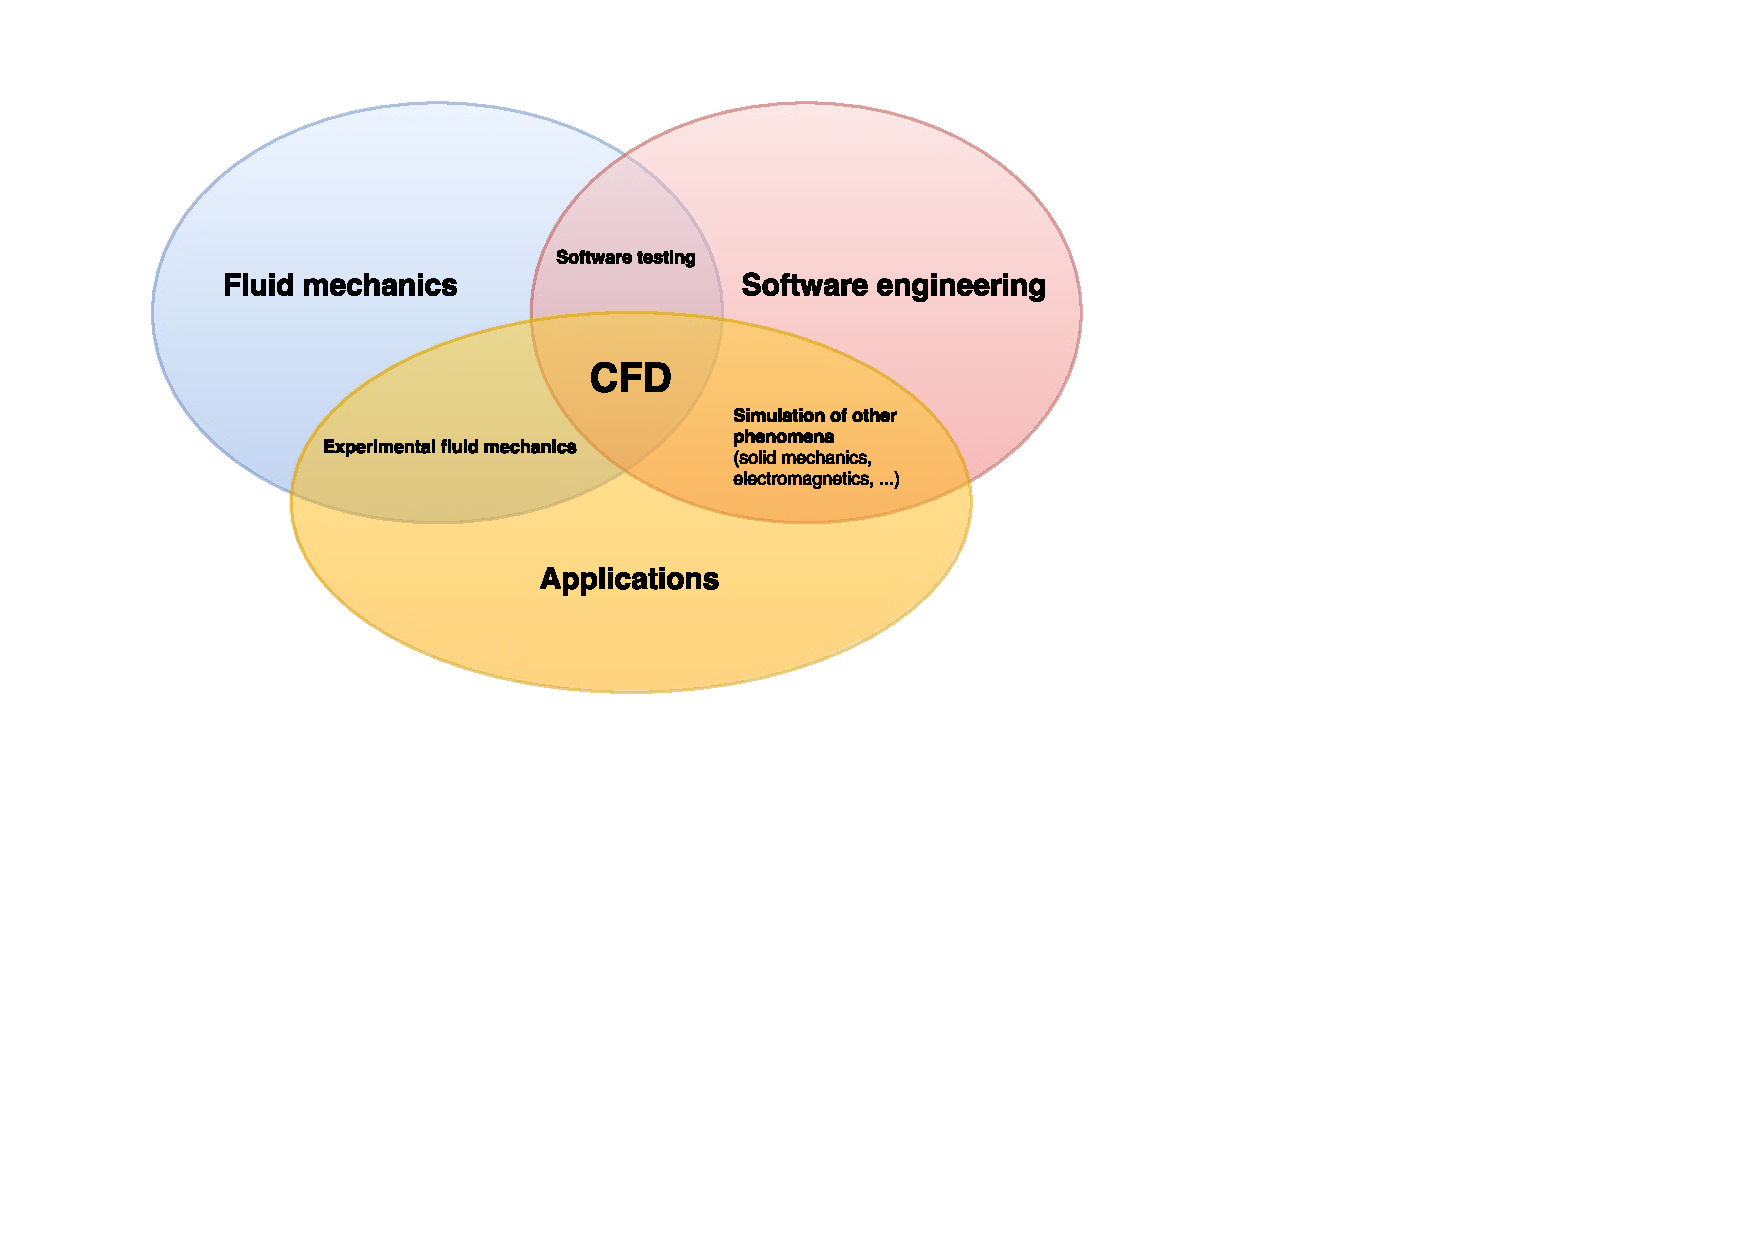
\includegraphics[trim=2cm 9cm 11cm 1cm,clip=true,width=0.7\textwidth]{Figures/Chapter1/CFD_scheme}
	\caption{Topics that conform CFD.}
	\label{fig-CFD}
\end{figure}

%Industrial problems
The CFD is widely used in many disciplines and industries like in the aerospace, automotive, chemical manufacturing, power generation, petroleum exploration, medical research, meteorology or astrophysics. It is a very valuable tool since it let to reductions in the cost of production by reducing the need of physical experimentation, improving the products or optimizing the production processes. In Table \ref{table-CFD_applications} we enumerate some more specific applications of CFD simulations that are very usefull for different disciplines.
\begin{table}[h]
\centering
\begin{tabular}{ll}
\toprule
Field&Application\\
\midrule
\midrule
\multirow{8}{*}{Biomedical}&Heart pumping\\
&Blood flow\\
&Air flow in lungs\\
&Nose and sinus flows\\
&Cell-fluid interface\\
&Artificial organ design\\
&Cardiac valve design\\
&Life support systems\\
\midrule
\multirow{1}{*}{Electronics}&Cooling flow in electronic devices\\
\midrule
\multirow{6}{*}{Aerospace and automotive}&Aerodynamic shape optimization\\
&Aerodynamic loads computation\\
&Turbines\\
&Propulsion systems\\
&Airbag Deployment\\
&In-Cylinder Engine Flow\\
\midrule
\multirow{4}{*}{Energy and power industry}&Heat exchange modeling\\
&Wind turbines blade design\\
&Pulverized coal combustion\\
&Emission of NOx particles\\
\midrule
\multirow{4}{*}{Environmental}&Impact of industrial exhausts\\
&Fire and smoke in buildings and tunnels\\
&Natural ventilation systems design\\
&Meteorology prediction\\
\midrule
\multirow{4}{*}{Civil}&Effect of wind on structures\\
&Water flow in rivers\\
&Water management\\
\bottomrule
\end{tabular}
\caption{CFD applications.}
\label{table-CFD_applications}
\end{table}

There already are CFD codes, both commercial and open source, that have the potential to solve a very broad spectrum of flow problems. However, the developement of computational algorithms for the simulation of turbulent flows is still an open topic. Moreover, the improvement of accuracy, the reduction of computational time and the increase of accessibility are also ongoing objectives in CFD. It is true that the CFD has some limitations, but the economic value of industrial applications has been demonstrated in a variety of industries.

%FE methods as CFD
The simulation of fluid flows relies on the fact that we can define a mathematical model that describes the fluid motion. The governing equations of the fluid dynamics are the Navier-Stokes equations. Then, the CFD basically consists on approximate the solution of these equations. Many approximation techniques can be used to simulate fluid flows, the most common are the Finite Element (FE) method, the Finite Differences (FD) method or the Finite Volume (FV) method. All of them are methods that can approximate the solution of a fluid flow and vary in the way in which the spatial domain is dicretized. 

The FD method is based on the application of a local Taylor expansion to approximate the governing equations, but it can only be applied on a discretization constructed by a network of topological squares or hexahedras, depending on the spatial dimensions. On the other hand, FE and FV methods are not restricted by this condition and are more extended in the CFD world. The FV method is based on the approximation of the average integral value on a reference volume being one of the main strengths the ability to handle discontinuous solutions. Rather than an integral average, the FE method is based on pointwise approximations on a grid. In contraposition to FV, it allows the use of high-order approximations and has a strong mathematical foundation behind.

In this thesis the FE method will be considered to discretize in space the Navier-Stokes equations. In any case, it has to be highlighted that the FV method can be recovered with a particular definition of the FE method.

%Exascale computing
The increasing computing power is one of the points that make not only the CFD, but also the computational mechanics in general, more appealing to solve engineering problems with more and more complexity. In order to take advantage of the continuously growing computational power acquired with the new improvements on super-computers, an advance in software design is imperative. New algorithms need to be designed to be used in the exascale computing environment. 

We understand by exascale computing the capacity of a computing system to perform at least one exaFLOPS ($ 10^{18} $ floating point operations per second). This computing capacity is still far from the current computer power, but many effords are dedicated to achieve this objective, which is expected to be acomplished before 2020. There are many issues in the High Performance Computing (HPC) community to be addressed in order to achieve the exascale goal. Some of them are related to the hardware development, including improvements on processors, memory size, memory bandwidth and energy consumtion. Furthermore, there is the need of software improvement in such a way that exascale computing systems can be fully exploited.

Exascale computing is the key with wich we will be able to perform high-fidelity simulations of real world problems. Such simulations are a great challenge of computational physics and engineering, and can transform the computational science into a fully predictive science.

%Large scale solvers
We still do not know much details about how exascale computing systems will be, but there is a clear priority in what software development refers. This is the definition and implementation of algorithms able to scale in extremely large computing environments (machines of the order of some million-cores). We recall here that an scalable algorithm has the property to have a computational cost proportional to the size of the problem that is being solved. Other numerical issues that are thought to be needed to achieve exascale computations are the use of high-order methods which give more accurate results for a given problem size and the development of adaptive methods, which can improve the efficiency of the simulation.

The application of a FE method to a Partial Differential Equation (PDE) leads to a matricial system of equations that has to be solved using linear algebra tools. The development of large scale FE solvers is accomplished by the use of preconditioners that improve the resolution of such matricial system. The most known algorithmically scalable preconditioners are the MultiGrid (MG) preconditioner and the Domain Decomposition (DD) based preconditioners. Nevertheless, in order to reach extreme scalabilty, the algorithmical scalability of a preconditioner is not a sufficient condition, since an efficient implementation is needed. 

%COMFUS group
The development of algorithms and implementations of scalable preconditioners is a hot topic in the FE field, and one of the main topics of the COMFUS team. The COMFUS group is the group where this thesis has been developed, and its name is the acronym of 

% (COMFUS group) in different lines of research, all of them related with the Starting Grant project of the European Research Council (ERC) headed by professor Santiago Badia.The objective of the COMFUS group is to develop significant advances on the simulation of the technology needed for the nuclear fusion. 




%From a technological point of view, nuclear fusion is considered as a safe and clean source of energy. In order to satisfy the future and increasing energetic needs of the society, there is the necessity  of efficient energy sources with a low $CO_2$ discharge. The increasing demand of energy sources that satisfy these conditions make nuclear fusion a strategic commitment for the EU energetic future.
%
%To make this energy source feasible, there must be a huge industrial development of the technology needed for its generation. The significance of the development of such technology arises with the creation of plans and European commissions such as the European Commission in the European Fusion Programme. This programme controls the construction and its subsequent experimentation of the experimental reactor ITER (International Thermonuclear Experimental Reactor). ITER will not be a completed fusion reactor, but it will allow to validate different concepts and technology needed to achieve the first fusion reactor able to provide energy efficiently, DEMO (DEMOnstration power plant). It is expected that ITER will be partially operative in 2017, but some tests such as the Tritium extraction will not be able to be performed until 2027. This date is too far given that the DEMO reactor is expected to be operative in the 2040 decade. This disadvantage explains the increasing need of numerical tools able to simulate the physical processes that occur in the nuclear fusion reactor. For instance, the European commission for the nuclear fusion development, Fusion for Energy (F4E), is opening constantly new calls for numerical investigations that allow the development of the needed technology. Currently, F4E is collaborating with the group where this thesis is being developed (COMFUS group) in different lines of research, all of them related with the Starting Grant project of the European Research Council (ERC) headed by professor Santiago Badia. 
%
%The objective of the COMFUS group is to develop significant advances on the simulation of the technology needed for the nuclear fusion. In this direction, the thesis is planed over the line of the development of numerical algorithms and computational tools able to simulate unsolved technological problems such as: 1) the plasma disruptions and magnetic confinement for large tokamaks and 2) the neutron shielding and the Tritium extraction inside the Test Blanket Modules (TBM). 

\section{Thesis objectives}

Residual-based VMS as LES

Mixed VMS formulations for LES

High-order FE methods

High-order time integration methods

Segregation of velocity-pressure

Adaptive time integration schemes

Large scale FE solvers

Scalable solvers

Application

The TBMs that wrap the fusion reactor core are a fundamental part of it. These modules not only are the responsible of the shielding that absorb the neutrons that emerge from the plasma, but also are the place where the Tritium is extracted. Tritium is needed to keep the plasma and it can not be found in nature, so its extraction is a key step. One of its design consists on a micro-channel system full of  liquid metal. Because of the magnetic forces that confine the plasma inside the reactor core, this liquid is subjected to the magnetohydrodynamics (MHD) equations.

As said before, these components can not be tested in ITER before 2027. When this occurs, its configuration will not be the same that the needed for the DEMO reactor. Then, the tests done in ITER reactor will mainly be used as a validation of the numerical simulation codes that will be used in the final design of the TBMs for the DEMO reactor.

These conditioning aspects imply that the research on numerical simulations able to reproduce such processes are a key step in the development of the nuclear fusion energy. In this thesis project we will continue the work of the COMFUS group in this line.

The liquid metals are electrical conductors that are subjected to the MHD physical laws, which couple the Navier-Stokes equations with Maxwell equations. These flows have a particular behaviour due to the magnetic effects. For a low magnetic Reynolds, the energy spectra is different of the defined by the classical flow theory. For this reason, it is necessary to \emph{develop numerical models able to simulate the quasi2D turbulence} that appears in these processes.

The stabilized finite element formulation for incompressible MHD, tested in laminar regime, that will be used in this thesis has been proposed recently by the group where this thesis is developed. The main novelty with respect to existent formulations is the use of the same interpolation for the fluid-dynamic and magnetic problems, keeping the optimal convergence. At this point, we want to explore its extension to turbulent cases by the use of Variational MultiScale (VMS) methods. These methods arise as a numerical stabilization techniques, but also model successfully the classical flow turbulence since they introduce numerical dissipation efficiently. Therefore, we firstly will \emph{test these methods in classical turbulent flows} to verify their applicability to a more complex turbulent flows. From this point, we want to apply the same methods to simulate the liquid metal problem, which is influenced by the magnetic field, and reproduce accurately the quasi2D turbulence.

The applications we have in mind are extremely complex and require large computational resources. The largest supercomputers are distributed-memory machines with thousands of cores. It is a very hard task to efficiently run simulation codes on these platforms. It requires excellent implementations and robust solvers, based on efficient preconditioners and Krylov solvers. The COMFUS team is actively working in this area, and the FEMPAR code developed by the team has already proved excellent scalability results up to 30,000 cores. The solvers used by the team combine robust and scalable solvers for symmetric positive definite problems and block-preconditioning. This approach allows to deal with indefinite problems like the Stokes system and fluids at low Reynolds numbers. However, there is still the challenge to scale up nonsymmetric and indefinite problems. In order to do so, we are forced to implement and \emph{develop novel techniques for nonsymmetric problems}.

The team has been actively working on new block preconditioners for inductionless and resistive MHD systems. These preconditioners, based on inexact-block LU factorizations, are used in combination with Krylov methods. Since these preconditioners are computationally intensive, it would be very appealing to use them as solvers instead of preconditioners. This approach, in the frame of resistive MHD has been exploited in \cite{badia_unconditionally_2012}, where the $\theta$ scheme was used for time integration. We plan to develop novel operator splitting methods based on implicit-explicit Runge-Kutta schemes. In particular, we want to \emph{design schemes that split velocity-pressure computations}.

Finally and related to the use of VMS methods, we want to \emph{test the advantages of the symmetric projection stabilization methods} with respect to classical VMS formulations.
%Besides to use these block preconditioners to solve the multiphysic problems, this thesis proposal also expect to use the block preconditioners structure to develop new time integrators which decouples the different physical problem variables. The idea is to take advantage of the Implicit-Explicit (IMEX) time integration technique using a Runge-Kutta scheme and operate with the different blocks to decouple the different physical fields that appears into the problem.
%
%\subsection{Large scale computation}
%As it has been said before, the physical processes that takes place in a nuclear fusion reactor lead to complex systems of equations. Besides the coupling between different physical problems, there also appear several length and time scales, resulting in a multi-scale problems. The way to solve accurately problems with large time scales without having numerical inestabilities and without using a small really time step, is by implicit methods. However, these methods require to solve nonlinear systems at each time-step. Then, there arise the need to use scalable solvers for massivelly parallel computers.
%
%It has to be said that the COMFUS group has an extensive experience in this topic. The code that will be used by the thesis development is designed to be used in distributed computers and it incorporates domain decomposition (DD) methods optimal for large scale problems that can be combined in a natural way with block preconditioners. The scalability of these methods has been proved to be excellent until 4096 CPUs {\color{red}(o mes??)}.
%
%To this end, this thesis project considers:
%\begin{itemize}
%\item {\bf Block preconditioners implementation and computational aspects}. As was said before, the multiphysical problem can be rewritten as a block system, i. e., one block for each unknown of the global problem. The non-diagonal blocks are those which couples the different subproblems. Here, the key decision is how to reorganize the system and subsequently how to define a good approximation to the original matrix, which will be used as a preconditioner. These preconditioners must be spectrally equivalent to the original matrix of the system of equations.
%
%{\color{red}... (Santi, queda alguna cosa a fer en aquest apartat? Em sembla que tot el que vam posar a la proposta de la FPU es lo que ja heu fet amb l'Alberto i el Ramon)}
%
%\item {\bf Domain Decomposition solvers for convection dominated flows}. {\color{red} ... (Aquest apartat no hi era a la proposta FPU, però l'he posat per mencionar lo del BDDC. Alguna idea per posar aqui?)}
%\end{itemize}

\section{Document structure}
 
% PRELIMINARIES

\chapter{Preliminaries}
\label{chap-Preliminaries}

%----------------------------------------------------------------------------------------

% Define some commands to keep the formatting separated from the content 
\newcommand{\keyword}[1]{\textbf{#1}}
\newcommand{\tabhead}[1]{\textbf{#1}}
\newcommand{\code}[1]{\texttt{#1}}
\newcommand{\file}[1]{\texttt{\bfseries#1}}
\newcommand{\option}[1]{\texttt{\itshape#1}}

%----------------------------------------------------------------------------------------

\section{The Governing equations of Fluid Mechanics}
\label{sec-C2_gov_eq}
In this section we will briefly state the basic concepts that one has to know about fluid mechanics and its mathematical description, which will be used in the forthcoming chapters.

Let us start with a review of the equations that govern the fluid flow. In this thesis we will restrict to constant-property Newtonian fluids. 

\subsection{The momentum equation}
\label{subsec-momentum}
From the Newton's second law, the momentum equation relates the fluid particle acceleration, $\frac{D\u}{Dt}$, to the external forces acting on such fluid particle. The external forces can be decomposed into the surface forces and the body forces, $\f$. The surface forces are described by the stress tensor $\boldsigma(\x,t)$ that is symmetric and, for constant-property Newtonian fluids, is defined by
\begin{equation}
\label{eq-stress_tensor_def}
\boldsigma = -\breve{p}\boldI + 2\mu\boldsymbol{\varepsilon}(\u), 
\end{equation}
where $\breve{p}$ is the pressure field, $\boldI$ the identity tensor, $\mu$ the viscosity, $ \u $ the fluid velocity and $\boldsymbol{\varepsilon}(\u)$ the strain rate tensor, which is defined by the following expression
\begin{equation}
\label{eq-strain_tensor_def}
\boldsymbol{\varepsilon}(\u)=\frac{1}{2}\left[\nabla\u+\left(\nabla\u\right)^T\right].
\end{equation}

The acceleration of the fluid particle is caused by the external forces according to the momentum equation
\begin{equation}
\label{eq-momentum_equation_def1}
\rho\frac{D\u}{Dt}=\nabla\cdot\boldsigma+\rho\f,
\end{equation}
being $\rho$ the density of the flow. Introducing the definition of the stress tensor \Eq{stress_tensor_def} into \Eq{momentum_equation_def1}, and dividing by the density $\rho$, which we consider to be constant, we get an alternative expression of the momentum equation
\begin{equation}
\label{eq-momentum_equation_def2}
\frac{D\u}{Dt}=-\nabla p+\nabla\cdot(2\nu\boldsymbol{\varepsilon}(\u))+\f,
\end{equation}
where we have used that $(1/\rho)\nabla\breve{p}=\nabla(\breve{p}/\rho)=\nabla p$, being $p:=\breve{p}/\rho$ the kinematic pressure, and $\nu=\mu/\rho$ the kinematic viscosity.

\subsection{Mass conservation}
\label{subsec-mass_conservation}
Matching the rate of change of mass in a given volume and the net mass flux across the boundary of such volume, and using the divergence theorem, we get the mass conservation or continuity equation, which is given by 
\begin{equation}
\label{eq-continuity_equation_def1}
\frac{\partial\rho}{\partial t}+\nabla\cdot(\rho\u)=0,
\end{equation}
which for constant density can be simplified to the kinematic condition that the velocity field be solenoidal or, what is the same, divergence-free:
\begin{equation}
\label{eq-continuity_equation_def2}
\nabla\cdot\u=0.
\end{equation}
Equation \Eq{continuity_equation_def2} is also called incompressibility constraint, since it is a constraint on the fluid velocity.

\subsection{Navier-Stokes equations}
\label{subsec-NS_equations}
Let $\Omega$ be a bounded domain of $\mathbb{R}^d$, where $d=2,3$ is the number of space dimensions, $\Gamma=\partial\Omega$ its boundary and $(0,T]$ the time interval. The strong form of the steady Navier-Stokes problem that govern the fluid flow motion consists of finding the velocity field $\u$ and the pressure field $p$ such that 
\begin{align}
\label{eq-NS_strong_momentum}
\frac{\partial\u}{\partial t}+\u\cdot\nabla\u-\nu\Delta\u+\nabla p=\f&\quad\mbox{in }\Omega\times(0,T],\\
\label{eq-NS_strong_continuity}
\nabla\cdot\u=0&\quad\mbox{in }\Omega\times(0,T],
\end{align}
where the decomposition of the velocity material derivative into the temporal partial derivative plus the convective derivative, $\frac{D\u}{Dt}=\frac{\partial\u}{\partial t}+\u\cdot\nabla\u$, and the fact that the velocity field is solenoidal have been used to simplify the momentum equation \Eq{momentum_equation_def2} into \Eq{NS_strong_momentum}. In forthcoming sections, the temporal partial derivative $ \frac{\partial(\cdot)}{\partial t} $ will also be denoted as $ \partial_t(\cdot) $.

Equations \Eq{NS_strong_momentum} and \Eq{NS_strong_continuity} need to be supplied with appropriate boundary and initial conditions. The boundary $\Gamma$ is divided into the Dirichlet ($\Gamma_D$) and the Neumann ($\Gamma_N$) parts such that $\Gamma_D\cup\Gamma_N=\Gamma$ and $\Gamma_D\cap\Gamma_N=\emptyset$. Then, the boundary and initial conditions can be written as
\begin{align}
\label{eq-NS_strong_Dir}
\u&=\u_g&\mbox{on $\Gamma_D\times(0,T]$,}\\
\label{eq-NS_strong_Neu}
(-p\mathbf{I}+\nu(\nabla\u+\nabla\u^T))\cdot\mathbf{n}&=\mathbf{t}_N&\mbox{on $\Gamma_N\times(0,T]$,}\\
\label{eq-NS_strong_Ini}
\u(\x,0)&=\u_0(\x)&\mbox{in $\Omega\times\{0\}$,}
\end{align}
$\mathbf{n}$ being the unit outward vector normal to $\Gamma$. For a solid wall, the velocity field on the Dirichlet boundary $\Gamma_D$ is governed by two conditions. The first of them is the no penetration condition, the flow cannot penetrate the wall.
\begin{equation}
\label{eq-NS_no_penetration}
\u\cdot\n=0\quad\mbox{on $\Gamma_D\times(0,T]$}.
\end{equation} 
For the tangential velocity components we impose the so called no-slip condition, which means that there is no relative movement between the wall and the fluid.
\begin{equation}
\label{eq-NS_no_slip}
\u\cdot\t=0\quad\mbox{on $\Gamma_D\times(0,T]$},
\end{equation}
being $\t$ a unit vector tangential to the wall. Putting together equations \Eq{NS_no_penetration} and \Eq{NS_no_slip} we have that $\u=\mathbf{0}$ on $\Gamma_D\times(0,T]$. If the wall is moving with a velocity $\u_g$ we recover the Dirichlet boundary condition \Eq{NS_strong_Dir}.

\subsection{Pressure and mass conservation}
\label{subsec-pressure_mass_conservation}
Let us now focus on the role that pressure field has in the fluid flow equations. If we take the divergence of the momentum equation \Eq{NS_strong_momentum}, assuming that the continuity equation \Eq{NS_strong_continuity} is not satisfied ($\nabla\cdot\u=\epsilon$), we have
\begin{equation}
\label{eq-NS_div_momentum}
\left(\frac{\partial}{\partial t}-\nu\Delta\right)\epsilon=-\Delta p-\nabla\cdot(\u\cdot\nabla\u).
\end{equation}
Considering problem \Eq{NS_div_momentum} with the initial condition $\epsilon_0=0$, we can say that the velocity field will be solenoidal ($\epsilon=0$) if, and only if, the following Poisson problem is satisfied
\begin{equation}
\label{eq-NS_poisson}
\Delta p=-\nabla\cdot(\u\cdot\nabla\u).
\end{equation}
Hence, we can state that the satisfaction of the Poisson problem \Eq{NS_poisson} is a necessary and sufficient condition for a solenoidal velocity field to remain solenoidal, see~\cite{pope_turbulent_2000}. Furthermore, for infinite domains, the solution of \Eq{NS_poisson} using the Biot-Savart law is given by 
\begin{equation}
\label{eq-NS_poisson_solution}
p(\x,t)=\frac{1}{4\pi}\int_\Omega\frac{\nabla\cdot(\u(\mathbf{y},t)\cdot\nabla\u(\mathbf{y},t))}{|\x-\mathbf{y}|}d\mathbf{y}.
\end{equation}
An important consequence of \Eq{NS_poisson_solution} is that the pressure field is non-local, that means that a fluctuation at one point $\mathbf{y}$ affects to the hole domain. A direct repercussion of the non-locality of the pressure is that the pressure waves sent from $\mathbf{y}$ induce far-field pressure forces ($-\nabla p$) that can agitate the fluid motion at large distances from that point. Then, every part of the flow feels every other part. This consequence is more relevant in the case of turbulent fluid flows, where eddies at different locations of the flow can interact each other. 


\section{The function spaces}
\label{sec-C2_functional_spaces}
Before describing the variational formulation of Navier-Stokes equations we need an introduction to some functional spaces. In this section we define the notation used in following sections and we give some definitions of fundamental function spaces. A deeper explanation of the concepts introduced in this section can be found in any functional analysis text, for example we refer to \cite{temam}, where we find a numerical analysis for the Stokes and Navier-Stokes equations.

Let us start considering $\Omega$ to be an open set of $\mathbb{R}^n$ with boundary $\Gamma$. Otherwise stated, we assume that the boundary of $\Omega$ is locally Lipschitz. We denote by $L^p(\Omega)$, with $1<p<+\infty$ (or $L^\infty(\Omega)$), the space of real functions defined on $\Omega$ with the $p$-th power absolutely integrable (or essentially bounded real functions for the case $p=\infty$). This is a Banach space with the norm 
$$\|\u\|_{L^p(\Omega)}:=\left(\int_\Omega|\u(\x)|^pd\Omega\right)^{\frac{1}{p}}$$
(or, for $p=\infty$,
$$\|\u\|_{L^\infty(\Omega)}:=\underset{\Omega}{\mbox{ess. sup}}|\u(\x)|).$$
For $p=2$, $L^2(\Omega)$ is a Hilbert space with the scalar product
$$(\u,\v)_\Omega:=\int_\Omega\u(\x)\v(\x)d\Omega.$$
Henceforth, when considering the scalar product over all domain $\Omega$ we will exclude the subscript, reading $(\cdot,\cdot)$. Furthermore, in forthcoming sections, the $L^2(\Omega)$-norm will be simply denoted as $\|\cdot\|$.
The Sobolev space  $W^{m,p}(\Omega)$ is the space of functions in $L^p(\Omega)$ with derivatives of order less than or equal to $m$ in $L^p(\Omega)$, being $m$ an integer and with $1\leq p\leq+\infty$. This is a Banach space with the norm
$$\|\u(x)\|_{W^{m,p}(\Omega)}:\left(\sum_{j\leq m}\|D^j\u(\x)\|^p_{L^p(\Omega)}\right)^{\frac{1}{p}},$$
where $D^j$ is the differentiation operator. When $p=2$, $W^{m,2}(\Omega)=H^m(\Omega)$ is a Hilbert space with the scalar product
$$(\u,\v)_{H^m(\Omega)}:=\sum_{j\leq m}\left(D^j\u,D^j\v\right).$$
Often we are concerned about $n$-dimensional vector functions with components in one of the spaces defined above. In this case we use bold characters to denote a vectorial space
$$\Lbf^p(\Omega):=\{L^p(\Omega)\}^n,\quad\Hbf^m(\Omega):=\{H^m(\Omega)\}^n.$$

Let $\Dcal(\Omega)$ be the space of $\Ccal^\infty$ functions with compact support contained in $\Omega$. The closure of $\Dcal(\Omega)$ in $H^m(\Omega)$ is denoted by $H^m_0(\Omega)$. The space $H^m_0(\Omega)$ can be though as the space of functions that belong in $H^m(\Omega)$ that vanish on the boundary $\Gamma$ in a general sense. Functions that belong to $H^m_0(\Omega)$ satisfy the Poincaré inequality
\begin{equation}
\label{eq-Poincare_inequality}
\|u\|\leq c(\Omega)\|\nabla\u\|,\quad\forall\u\in\Hbf^m_0(\Omega).
\end{equation}

From a physical point of view, as noticed in \cite{Foias}, we can think on the space $\Lbf^2(\Omega)$ as the space of all vector fields $\u$ with finite kinetic energy. Moreover, the $\Hbf^1(\Omega)$ can be though as the space of all vector fields $\u$ with finite enstrophy.

Let us consider some additional spaces that are useful in the mathematical description of the Navier-Stokes equations. A possible way to deal with the incompressibility constrain \Eq{NS_continuity} is to consider a functional space with less regularity than $\Hbf^1(\Omega)$ defined as
$$\Hbf(div,\Omega):=\{\u\in\Lbf^2(\Omega)|\nabla\cdot\u\in\Lbf^2(\Omega)\},$$
which is a Hilbert space with the norm
$$\|\u\|_{div}:=\|\u\|+\|\nabla\cdot\u\|.$$
The closure of $\Dcal(\Omega)$ in $\Hbf(div,\Omega)$ is denoted by $\Hbf_0(div,\Omega)$.
...

\subsection{The set $\Omega$}

\subsection{$L^p$ and Sobolev spaces}

\subsection{}

\section{The variational formulation}
\label{sec-C2_variational}
\subsection{Continuous formulation}
\label{subsec-variational_continuous}
Let us consider the strong form of the Navier-Stokes problem \Eq{NS_strong_momentum}-\Eq{NS_strong_Ini}. In order to formulate the equivalent variational problem we define a set of variational spaces that incorporates the homogeneous Dirichlet boundary condition and the temporal evolution
\begin{align}
\label{eq-C2_varia_NS_u_space}
&\mathcal{V}_g:=\left\{\v\in\Hbf^1(\Omega):\left.\v\right|_{\Gamma_D}=\u_g\right\}\equiv\Hbf^1_g(\Omega),\\
\label{eq-C2_varia_NS_v_space}
&\mathcal{V}_0:=\left\{\v\in\Hbf^1(\Omega):\left.\v\right|_\Gamma=0\right\}\equiv\Hbf^1_0(\Omega),\\
\label{eq-C2_varia_NS_p_space}
&\mathcal{Q}:=\Lbf^2(\Omega)/\mathbb{R}.
\end{align}
Given sufficiently smooth functions $ \v\in\mathcal{V}_0 $ and $ q\in\mathcal{Q} $, we obtain the variational or weak version of the Navier-Stokes equations multiplying \Eq{NS_strong_momentum} by $ \v $  and \Eq{NS_strong_continuity} by $ q $, integrating over $ \Omega $ and integrating by parts the second order derivatives. Then the variational Navier-Stokes problem reads: find $ \u\in\Lbf^2(0,T;\mathcal{V}_g),\\ $ and $ p\in\Lbf^1(0,T;\mathcal{Q}) $ such that: 
\begin{align}
\label{eq-C2_varia_NS_weak_momentum}
(\partial_t\u,\v)+\left(\nu\left(\nabla\u+\nabla\u^T\right),\nabla\v\right)+b(\u,\u,\v)+(\nabla p,\v)=&\left\langle f,\v\right\rangle&\forall\v\in\mathcal{V}_0,\\
\label{eq-C2_varia_NS_weak_continuity}
(\nabla\cdot\u,q)=&\ 0&\forall q\in\mathcal{Q}.
\end{align}
Adding up equations \Eq{C2_varia_NS_weak_momentum}-\Eq{C2_varia_NS_weak_continuity} we obtain an alternative weak form of the incompressible Navier-Stokes problem \Eq{NS_strong_momentum}-\Eq{NS_strong_Ini} consists, e.g., in finding $[\u,p]\in {L}^2(0,T;\mathcal{V}_g)\times {\cal D}'(0,T;\mathcal{Q})$ (distributions in time with values in $\mathcal{Q}_0$) such that
\begin{equation}
\label{eq-C2_NS_weak}
(\partial_t\u,\v) + B(\u;[\u,p],[\v,q]) = \left<\f,\v\right> 
\quad\quad\forall\v\in\mathcal{V}_0,\quad\forall q\in\mathcal{Q},
\end{equation}
satisfying the initial condition \Eq{NS_strong_Ini} in a weak sense. Here the form $B({\a};[\u,p],(\v,q))$ is defined as 
\begin{equation}
\label{eq-C2_bilinear}
B(\a;[\u,p],[\v,q]):=\nu(\nabla\u,\nabla\v)+b(\a,\u,\v)-(p,\nabla\cdot\v)+(q,\nabla\cdot\u)
\end{equation}
where the trilinear weak form of the convective term $b(\u,\v,\w)$ can be written in the following three equivalent ways
\begin{align}
\label{eq-C2_b_noskew}
&b(\u,\v,\w)=(\u\cdot\nabla\v,\w)&&\mbox{Non conservative},\\
\label{eq-C2_b_skew1}
&b(\u,\v,\mathbf{w})=\frac{1}{2}(\u\cdot\nabla\v,\mathbf{w})-\frac{1}{2}(\v,\u\cdot\nabla\mathbf{w})&&\mbox{Skew-symmetric (type 1)},\\
\label{eq-C2_b_skew2}
&b(\u,\v,\mathbf{w})=(\u\cdot\nabla\v,\mathbf{w})+\frac{1}{2}(\v\cdot\mathbf{w},\nabla\cdot\u)&&\mbox{Skew-symmetric (type 2)}.
\end{align}
Note that in the trilinear weak forms \Eq{C2_b_noskew}-\Eq{C2_b_skew2} the boundary integral terms that arise from the integration by parts have been neglected. This assumption is valid when strong Dirichlet boundary conditions are considered over all the boundary. Despite of that, this equivalence is lost at the discrete level. The skew-symmetric form (type 2) (\ref{eq-C4_b_skew2}) is very common when numerical analysis are presented ~\cite{badia_convergence_2014,burman_galerkin_2009,guermond_faedogalerkin_2007} but the skew-symmetric form (type 2) (\ref{eq-C4_b_skew1}) has important advantages when the first argument is a discontinuous function, as will be shown in forthcoming chapters.

The well-posedness of problem \Eq{C2_NS_weak} relies on the called LBB condition, which stands for the name of the authors that developed works related to that condition. See the works by Ladyzhenskaya ~\cite{ladyzhenskaya1969mathematical}, Babu\^{s}ka ~\cite{babuska_error-bounds_1971} and Brezzi ~\cite{brezzi1974existence}. The LBB condition is also called \textit{inf-sup} condition and reads as follows: there exist a positive constant $ \beta $ such that,
\begin{equation}
\label{eq-C2_lbb}
\inf_{q\in\mathcal{Q}}\sup_{\v\in\mathcal{V}_0}\frac{(\nabla\cdot\v,q)}{\|\v\|_\mathcal{V}\|q\|_{\mathcal{Q}/\ker A^t}}\ge\beta>0,
\end{equation}
being $ A^t $ the adjoin of the operator defined as 
\begin{equation}
\label{eq-C2_lbb_operator}
A: \mathcal{V}_0\rightarrow\mathcal{Q'} \quad| \quad\langle A(\v),a\rangle_{\mathcal{Q'}\times\mathcal{Q}}=(\nabla\cdot\v,q)\quad\quad\forall\v\in\mathcal{V}_0,\quad\forall q\in\mathcal{Q}
\end{equation}

\subsection{The Finite Element method}
\label{subsec-variational_finite_element}
In order to approximate the solution of the variational problem \Eq{C2_NS_weak}, one needs to construct finite-dimensional spaces in which the solution can be computed. The approach followed in this work to construct such finite-dimensional spaces is the called Finite Element (FE) method. According to Ciarlet, see ~\cite{ciarlet_finite_1978}, we can define a FE as follows.

Let $ K\subseteq\Rbb^n $ be a bounded closed set with nonempty interior and piece-wise smooth boundary, the element domain. Let $ \mathcal{S} $ be a finite-dimensional space of functions on $ K $, the space of shape functions. Let $ \mathcal{N}=\{\mathcal{N}_1,\mathcal{N}_2,...,\mathcal{N}_k\} $ be a basis for $ \mathcal{S}' $, the set of nodal variables. Then, $ (K,\mathcal{S},\mathcal{N}) $ is called a FE.

We refer to Brenner et al ~\cite{brenner_mathematical_2007} for a deeper explanation of the FE definitions.

In this thesis we will mainly use FE spaces composed by quadrilateral finite elements built from a tensor product of polynomials. For the 3D case, we consider a reference FE $ (\widetilde{K},\widetilde{\mathcal{S}},\widetilde{\mathcal{N}}) $ with $ \widetilde{K} $ a cube defined in $ [-1,1]^3 $, $ \widetilde{\mathcal{S}}=Q_k $ being
$$ Q_k:=\left\{\sum_jc_jp_j(x)q_j(y)r_j(z):\mbox{ with $ p_j $, $ q_j $ and $ r_j $ polynomials of degree $j \leq k $}\right\}, $$
and $ \widetilde{\mathcal{N}} $ denoting the point evaluations at $ \left\{(t_l,t_m,t_n):\ l,m,n=0,1,...,k \right\} $ where \\$\left\{-1 = t_0 < t_1 < ... < t_k = 1 \right\}$.

Let us now consider a FE partition $ \mathcal{T}_h $ of the domain $ \Omega $ composed by a set of elements $ \left\{K_e\right\}_{e=1}^{ne} $, being $ ne $ the total amount of elements in the domain. Let us consider $ F_K $ a mapping from $ K $ to $ \widetilde{K} $, i. e. $ F_K(K)=\widetilde{K} $ with its pull-back map defined as $ F^*_K(\hat{f}):=\hat{f}\circ F_K $, see ~\cite{ciarlet_general_1972,brenner_mathematical_2007} for more details on equivalence between FE.

Then the FE spaces for the velocity and pressure fields equivalent to \Eq{C2_varia_NS_u_space}-\Eq{C2_varia_NS_p_space} can be defined as
\begin{align}
\label{eq-C2_varia_NS_vh_space}
&\mathcal{V}_{h}:=\left\{\v_h\in(\mathcal{C}^0(\Omega))^d:\left.\v_h\right|_K=\tilde{\v}\circ F_K^{-1},\ \tilde{\v}\in(Q_{k_v})^d,\ K\in\mathcal{T}_h\right\},\\
\label{eq-C2_varia_NS_vgh_space}
&\mathcal{V}_{g,h}:=\left\{\v_h\in\mathcal{V}_h:\left.\v_h\right|_{K\cap\Gamma}=\u_g\right\},\\
\label{eq-C2_varia_NS_v0h_space}
&\mathcal{V}_{0,h}:=\left\{\v_h\in\mathcal{V}_h:\left.\v_h\right|_{\partial K}=0\right\},\\
\label{eq-C2_varia_NS_qh_space}
&\mathcal{Q}_h:=\left\{\mathcal{C}^0(\Omega)\cap\Lbf^2(\Omega)/\mathbb{R}:\left.q_h\right|_K=\tilde{q}\circ F_K^{-1},\ \tilde{q}\in Q_{kq},\ K\in\mathcal{T}_h \right\}.
\end{align}
Where $ k_v $ and $ k_q $, not necessarily equal, are the degree of the polynomials used to define the interpolation space for the velocity and pressure fields, respectively. In what follows, the subindex $ h $ will denote functions related to the FE space. Note that in this work both velocity and pressure field spaces, $ \mathcal{V}_h $ and $ \mathcal{Q}_h $, are considered to be made by continuous functions in the same partition of the domain, $ \mathcal{T}_h $.

\subsection{Semi-discrete formulation}
\label{subsec-variational_semidiscrete}
Let us consider a FE partition $ \mathcal{T}_h $ of the domain $ \Omega $ from which we can construct conforming finite dimensional spaces for the velocity $\mathcal{V}_{g,h}\subset\mathcal{V}_g$, and for the pressure $ \mathcal{Q}_{0,h}\subset\mathcal{Q}_0 $. The spaces $\mathcal{V}_{g,h}$ and $ \mathcal{Q}_{0,h} $ are the ones defined in the previous section, equations \Eq{C2_varia_NS_vgh_space} and \Eq{C2_varia_NS_qh_space} respectively.

The Galerkin FE approximation of \Eq{C2_NS_weak} consists in finding $[\u_h,p_h]\in {L}^2(0,T;\mathcal{V}_{g,h})\times {\cal D}'(0,T;\mathcal{Q}_h)$ such that
\begin{equation}
\label{eq-C2_NS_weak_discrete}
(\partial_t\u_h,\v_h) + B(\u_h;[\u_h,p_h],[\v_h,q_h]) = \left<\f,\v_h\right> 
\quad\quad\forall\v_h\in\mathcal{V}_{0,h},\quad\forall q_h\in\mathcal{Q}_h,
\end{equation}

Problem \Eq{C2_NS_weak_discrete} is well posed if the discrete \textit{inf-sup} condition equivalent to \Eq{C2_lbb} is satisfied. The discrete version reads: there exist a positive constant $ \beta_d $, independent of $ h $, such that,
\begin{equation}
\label{eq-C2_lbb_discrete}
\inf_{q_h\in\mathcal{Q}_h}\sup_{\v_h\in\mathcal{V}_{0,h}} \frac{(\nabla\cdot\v_h,q_h)}{\|\v_h\|_{\mathcal{V}_h}\|q\|_{\mathcal{Q}_h/\ker A_h^t}}\ge\beta_d>0,
\end{equation}
with $ A_h $ the equivalent operator to the one defined in \Eq{C2_lbb_operator}.



\section{The Variational Multiscale method}
\label{sec-C2_vms}
Let us consider a FE partition $\mathcal{T}_h$ of the domain $\Omega$ from which we can construct conforming finite dimensional spaces for the velocity $\mathcal{V}_{0,h} \subset \mathcal{V}_0$, and for the pressure $\mathcal{Q}_{0,h}\subset \mathcal{Q}_0$. 

It is well known that the Galerkin FE approximation \Eq{NS_galerkin} has numerical instabilities for high mesh Reynolds number problems, i.e., when the nonlinear convective term dominates the viscous term. Another drawback of that formulation is the discrete \textit{inf-sup} condition that must be satisfied by the pair $\mathcal{V}_{0,h} \times\mathcal{Q}_{0,h}$ in order to have a well-posed problem with bounded pressure. These difficulties are overcome by using the VMS approach, introduced by Hughes in \cite{hughes,hughes}, and that is stated as follows.

Let us consider a two-scale decomposition of spaces $\mathcal{V}_0$ and $\mathcal{Q}_0$ such that $$\mathcal{V}_0=\mathcal{V}_{0,h}\oplus\widetilde{\mathcal{V}}_0$$ and $$\mathcal{Q}_0=\mathcal{Q}_{0,h}\oplus\widetilde{\mathcal{Q}}_0,$$ where $\widetilde{\mathcal{V}}_0$ and $\widetilde{\mathcal{Q}}_0$ are infinite-dimensional spaces that complete the FE spaces in $\mathcal{V}_0$ and $\mathcal{Q}_0$, respectively. Hereinafter the subscript $(\cdot)_h$ will denote the FE component and the tilde $\widetilde{(\cdot)}$ the subgrid component. Applying the two-scale decomposition to \Eq{NS_weak} we obtain a discrete problem
\begin{align}
\label{eq-C2_vms_NS_discrete}
(\partial_t\u_h,\v_h)+(\partial_t\tilde{\u},\v_h)&+B(\a;[\u_h,p_h],[\v_h,q_h])\\\nonumber
&+\left(\tilde{\u},\mathcal{L}_{\a}^*(\v_h,q_h)\right)_h-\left(\tilde{p},\nabla\cdot\v_h\right)=\left<\f,\v_h\right>,
\end{align}
where $(\cdot,\cdot)_h=\sum_{K\in\mathcal{T}_h}(\cdot,\cdot)_K$ is the sum of scalar products (\ref{eq:scalar_product}) over each element $K$ of the partition $\mathcal{T}_h$, and
\begin{equation}
\label{eq-C2_vms_adjoint}
\mathcal{L}_{\a}^*(\v_h,q_h):=-\nu\nabla^2\v_h-\a\cdot\nabla\v_h-\nabla q_h
\end{equation}
is the formal of the adjoint operator of the momentum equation. The term involving the adjoint operator comes from an elementwise integration by parts of the terms involving the subscales, in which the boundary terms 
$\left( \v_{h},\nu \n\cdot \nabla \tilde{\u}\right)_{\partial h}$ and
$\left( q_{h},\n\cdot \tilde{\u}\right)_{\partial h}$
have been neglected (the subscript ${\partial h}$ is used to denote the sum over all elements of the integral on the boundary of each element). It also involves the approximation 
$b(\a,\tilde{\u},\u_h) \approx -(\tilde{\u},\a\cdot\nabla\v_h)$
which implies neglecting 
$\left( \v_{h},\n\cdot \a \tilde{\u}\right)_{\partial h}$ and
$(\tilde{\u},\nabla\cdot\a\v_h)$. 
These approximations are discussed in  \cite{codina_time_2007} together with the choice of $\a$ which defines the type of scale splitting (linear or nonlinear), also discussed below.

The discrete problem depends on $\tilde{\u} \in \widetilde{\mathcal{V}}_0$ and on $\tilde{p}\in \widetilde{\mathcal{Q}}_0$,  $\widetilde{\mathcal{V}}_0$ and $\widetilde{\mathcal{Q}}_0$ being infinite-dimensional. Therefore, the equations for $\tilde{\u}$ and $\tilde{p}$ obtained after applying the two-scale decomposition cannot be directly solved, but some modeling steps are needed to obtain a feasible method. Considering the subscale as a time-dependent variable of the problem (see below) and approximating the Navier-Stokes operator by two stabilization parameters $\tau_m^{-1}$ and $\tau_c^{-1}$ (see for example \cite{codina_time_2007}), the fine scale problem can be written as
\begin{align}
\label{eq-C2_vms_velo_sgs}
\partial_t\tilde{\u}+\tau_m^{-1}\tilde{\u}=\mathcal{P}(\R_u),\\
\label{eq-C2_vms_press_sgs}
\tau_c^{-1}\tilde{p}=\mathcal{P}(R_p).
\end{align}
In \Eq{velo_sgs}-\Eq{press_sgs} $\mathcal{P}$ denotes the projection onto the space of subscales, which is discussed below. In turn, the vector $\R$ is the residual of the Navier-Stokes equations \Eq{NS_strong_mome}-\Eq{NS_strong_inc}, defined as $\R=[\R_u,R_p]^T$, with
\begin{align}
\label{eq-C2_vms_Ru}
%&\R_u=\f-\left(\partial_t\u_h+N((\u_h+\tilde{\u}),\u_h)+\nabla p_h \right),\\
%&\R_u=\f-\left(\partial_t\u_h+ \a \cdot \nabla \u_h + \nabla p_h \right),\\
&\R_u=\f-\partial_t\u_h-\mathcal{L}_{\a}(\u_h,p_h),\\
\label{eq-C2_vms_Rp}
&R_p=-\nabla\cdot\u_h.
\end{align}
where
\begin{equation}
\label{eq-C2_vms_operator}
\mathcal{L}_{\a}(\v_h,q_h):=-\nu\nabla^2\v_h+\a\cdot\nabla\v_h+\nabla q_h
\end{equation}
%and $N((\u_h+\tilde{\u}),\u_h)=(\u_h+\tilde{\u})\cdot\nabla\u_h$ is the convective term. 
Finally, the expressions of the stabilization parameter $\tau_m$ is 
\begin{align}
\label{eq-C2_vms_tau_m}
&\tau_m=\left(\frac{c_1\nu}{h^2}+\frac{c_2|\a|}{h}\right)^{-1},
\end{align}
whereas we consider two possible definitions of $\tau_c$, viz. $\tau_c = 0$ (which implies $\tilde{p} = 0$) and 
\begin{align}
\label{eq-C2_vms_tau_c}
&\tau_c=\frac{h^2}{c_1\tau_m},
\end{align}
where $h$ is the mesh size and $c_1$ and $c_2$ are algorithmic constants. Let us comment on expression \Eq{tau_m}:
\begin{itemize}
\item The influence of the constants $c_1$ and $c_2$ is discussed in Section XXXX. A theoretical way to determine them would be to impose that the numerical dissipation they introduce be equal to the molecular dissipation in turbulent regimes, as explained in~\cite{guasch-codina-13}. 
\item The definition of $\tau_m$ in \Eq{tau_m} is not standard, in the sense that the one used often depends on the time step size of the time discretization, $\delta t$. Instead of \Eq{tau_m}, $\tau_m^{-1}=\frac{1}{\delta t} + \frac{c_1\nu}{h^2}+\frac{c_2|\a|}{h}$ is more often considered (see, e.g., \cite{Hsu2010,gamnitzer_time-dependent_2010}). We refer to 
Section XXXX~\ref{sec:small_time_step} for a more detailed discussion about this topic. Likewise, other expressions with the same asymptotic behavior in terms of $h$, $\nu$ and $|\a|$ can also be employed.
\item Expression \Eq{tau_m} corresponds to linear isotropic elements. If elements of order $p$ are used ($p$ is not the pressure, here), $c_1$ must be replaced by $c_1 p^4$ and $c_2$ by $c_2 p$. For anisotropic elements, the definition of $h$ within each element is not obvious. A possibility is explained in \cite{Principe2010}.
\end{itemize}

In the following three sections we discuss the particular ingredients of our VMS models. A different summary can also be found in \cite{Codina-chap-2011}, together with some numerical experiments. 

\subsection{The dynamics of the subscales}
\label{subsec-C2_vms_dyn}
Stabilized formulations were originally developed for steady convection-diffusion \cite{Brooks_1982} and Stokes \cite{Douglas_1989,Hughes_1986_5} problems. As the numerical instabilities have a spatial nature, the time dependency of the subscales was not considered, and the standard choice \cite{Hughes2000,hughes_large_2001,bazilevs_variational_2007} was to take 
\begin{equation}
\label{eq-C2_vms_static_sgs}
\tilde{\u}=\tau_m \mathcal{P}(\R_u),
\end{equation}
that is, to neglect the temporal derivative of the subscales in (\ref{eq:velo_sgs}). In this case, the subscales are called quasi-static in what follows.

The subscale as a time dependent variable of the problem was introduced in \cite{codina_stabilized_2002,codina_time_2007}. It gives rise to important properties like commutativity of space and time discretization, stability without restrictions on the time step size \cite{codina_time_2007,Badia2009a} and, combined with orthogonal subscales, to convergence towards weak solutions of the Navier-Stokes equations \cite{Badia2013Convergence} and the possibility of predicting backscatter \cite{Codina-chap-2011,Principe2009}. 

Equation \Eq{velo_sgs} can be analytically integrated to give
\begin{equation}
\label{eq:exact_sgs}
\tilde{\u}(t^*)=\tilde{\u}(0) + \mu^{-1}(t^*) \int_0^{t^*} \mu(t) \mathcal{P}\R_u {\rm d}t, \quad \quad \mu(s)=\exp \int_0^s \tau^{-1}(t){\rm d}t,
\end{equation}
where it is explicitly seen that the subscale is a function of the residual but also of the flow history. In practice this integration is performed numerically, as described below.

\subsection{(Non)linear scale splitting}
\label{subsec-C2_vms_nl}
The original VMS formulation \cite{hughes_multiscale_1995,hughes_variational_1998} was developed having linear problems in mind and its extension to the Navier-Stokes equations was implicitly based on a ``linearization'', fixing the advection velocity and applying the multiscale splitting to the rest of the terms. A nonlinear scale splitting was used in \cite{Hughes2000,hughes_large_2001} together with an explicit resolution of the small scales in which a Smagorinsky damping was introduced. A nonlinear scale splitting with modeled subscales was used in \cite{codina_stabilized_2002, bazilevs_variational_2007} and in \cite{codina_time_2007}, where it was shown that it leads to global conservation of momentum. We therefore consider both options
%The vector $\a$ appearing in (\ref{eq:bilinear}) and (\ref{eq:adjoint}) is the advection velocity of the convective term. It can be defined in two different ways depending if we use a linear or a nonlinear scheme for the subscales definition. That is, 
\begin{align}
\label{eq-C2_vms_a_lin}
&\a=\u_h&&\mbox{for linear subscales},\\
\label{eq-C2_vms_a_nl}
&\a=\u_h+\tilde{\u}&&\mbox{for nonlinear subscales}.
\end{align}

\begin{remark}
\label{rem-skewsym}
When we use the nonlinear definition for the advection velocity, $\a=\u_h+\tilde{\u}$, the skew-symmetric term \textit{type 2} \Eq{b_skew2} in the FE equation \Eq{NS_discrete} reads: 
\begin{equation}
\label{eq-C2_vms_b_skew2_aux1}
b(\a,\u_h,\v_h)=((\u_h+\tilde{\u})\cdot\nabla\u_h,\v_h)+\frac{1}{2}(\u_h\cdot\v_h,\nabla\cdot\u_h)+\frac{1}{2}(\u_h\cdot\v_h,\nabla\cdot\tilde{\u}).
\end{equation}
The last term is not well-defined, since it includes derivatives of the discontinuous subscale $\tilde{\u}$. One possibility is to neglect it (as previously done with other similar terms when arriving to \Eq{NS_discrete}), which implies
\begin{equation}
b(\a,\u_h,\u_h)=-\frac{1}{2}(|\u_h|^2,\nabla\cdot\tilde{\u}),
\end{equation}
the same result obtained when the non conservative form is used.
By contrast, the skew-symmetric term \textit{type 1} in the FE equation \Eq{NS_discrete} reads
\begin{equation}
\label{eq-C2_vms_b_skew1_aux1}
b(\a,\u_h,\v_h)=\frac{1}{2}((\u_h+\tilde{\u})\cdot\nabla\u_h,\v_h)-\frac{1}{2}((\u_h+\tilde{\u})\cdot\u_h,\nabla\cdot\v_h)
\end{equation}
from where
\begin{equation}
b(\a,\u_h,\u_h)=0.
\end{equation}
% and we can not use the FE shape function derivatives to approximate it because the subscales are on another space. Then we avoid this problem by neglecting this term. 
%Therefore, the skew-symmetric term \textit{type 2} implementation for a nonlinear definition of the subscales will be
%\begin{equation}
%\label{eq:b_skew2_aux2}
%b(\a,\u_h,\v_h)=(\a\cdot\nabla\u_h,\v)+\frac{1}{2}(\u_h\cdot\v_h,\nabla\cdot\a)-\frac{1}{2}(\u_h\cdot\v_h,\nabla\cdot\tilde{\u}).
%\end{equation}
In Subsection XXXX(\ref{subsec:result_DHIT}) we will see the influence of the two forms of the convective term on the results.
It is worth noting that the same approximations have been introduced in all cases to implement $b(\a,\tilde{\u},\u_h)$, but these approximations are taken into account in the (usual) energy estimates of Section XXXX\ref{sec:energy}.
%Note that \textit{type 2} is the standard choice.
\end{remark}

\begin{remark}
At the continuous level, the different expressions of the convective term are also equivalent to the so called conservation form
\begin{align}
b(\u,\v,\w)= -(\u\otimes \v,\nabla\w).\nonumber
\end{align}
In the discrete problem, the nonlinear scale splitting leads to the following terms in the momentum equation:
\begin{align}
b(\a,\u_h +\tilde\u,\v_h)= - (\u_h\otimes\u_h, \nabla\v_h)
- (\u_h\otimes\tilde\u, \nabla\v_h)- (\tilde\u\otimes\u_h, \nabla\v_h)
- (\tilde\u\otimes\tilde\u, \nabla\v_h).\label{eq:nonconconv}
\end{align}
Even if this is not exactly what we get using the non-conservative or skew-symmetric forms because of the approximation error, this allows us to interpret the different contributions arising from the nonlinear scale splitting. As it is explained in \cite{Codina-chap-2011}, from (\ref{eq:nonconconv}) we can identify the contributions from the cross stresses, the Reynolds stresses and the subgrid scale tensor. 
\end{remark}

\subsection{The space for the subscales}
\label{subsec-C2_vms_oss}
The selection of the space for the approximation of the subscales determines the projection $\mathcal{P}$ appearing in the right-hand side of \Eq{velo_sgs} and \Eq{press_sgs}. The first option, already considered in \cite{Hughes2000,hughes_large_2001,bazilevs_variational_2007} and named Algebraic Subgrid Scale (ASGS) in \cite{codina_stabilization_2000} is to take the subscales in the space of the residuals, that is,
%method is characterized by the following projection definition:
\begin{equation}
\label{eq-C2_vms_P_ASGS}
\mathcal{P}:=\mathbf{I}.
\end{equation}
Another possibility introduced in \cite{codina_stabilization_2000} is to consider the space of the subscales orthogonal to the FE space. The main motivation of the method is that a stability estimate for the projection onto the FE space of the pressure and/or the convective terms can already be obtained in the standard Galerkin method and therefore the only ``missing'' part is the orthogonal one. The Orthogonal Subscales (OSS) method is then characterized by the following projection definition:
\begin{equation}
\label{eq-C2_vms_P_OSS}
\mathcal{P}:=\Pi_h^\bot=\mathbf{I}-\Pi_h,
\end{equation}
where $\Pi_h$ is the projection onto the FE space. With this choice, the residual of the momentum equation does not depend on $\partial_t\u_h$. Likewise, $\mathcal{P}(\f)$ in this case is only well defined for $\f\in L^2(\Omega)^d$. In the case of minimum regularity, $\f\in H^{-1}(\Omega)^d$, this term can be simply neglected without upsetting the accuracy of the method.

In fact, with this choice, the orthogonality between the space of subscales and the FE space is only guaranteed when the stabilization parameters are constant. If this is not the case, the method is still optimally convergent \cite{Codina_2008a} but this property is lost. In order to have truly orthogonal subscales, \emph{which guarantees a proper separation of the FE and the subgrid scale kinetic energies} (see below and Section \ref{sec:energy}) a slight modification of the projection $\Pi_h$ is needed (see \cite{Codina_2008a}). We will use two different weighted projections: one for the velocity subscales ($\Pi_m$) in \Eq{velo_sgs} and another for the pressure subscales ($\Pi_c$) in \Eq{press_sgs}. We define the weighted projections $\Pi_m$ and $\Pi_c$ such that given any vector $\w\in\mathcal{V}_0$ and any scalar $r\in\mathcal{Q}_0$ we have
\begin{align}
\label{eq-C2_vms_Pi_tau_m}
&(\tau_m\Pi_m(\w),\v_h)=(\tau_m\w,\v_h)&&\forall\v_h\in\mathcal{V}_{0,h},\\
\label{eq-C2_vms_Pi_tau_c}
&(\tau_c\Pi_c(r),q_h)=(\tau_cr,q_h)&&\forall q_h\in\mathcal{Q}_{0,h}.
\end{align}
These definitions guarantee the orthogonality between the FE and subscale spaces in the case of static subscales, that is, neglecting temporal derivatives in \Eq{velo_sgs}. It then follows that the term containing the temporal derivative of the subscale in the FE equation \Eq{NS_discrete} also vanishes.

However, if the dynamic version of the method is used, the weight of the projection \Eq{Pi_tau_m} must be conveniently modified to ensure the mentioned orthogonality. As it can be seen in XXXXX(\ref{eq:exact_sgs}), the definition of the weight depends on the time integration strategy, as explicitly stated in Section XXXX\ref{sec:discrete}.

\section{Time integration}
\label{sec-C2_time_integration}
In this section, our aim is to state some basic concepts about the time discretization. Once we have defined the semi-discrete problem, as it has been formulated in Section \ref{subsec-variational_semidiscrete}, we end up with an Ordinary Differential Equation (ODE), which has to be integrated in order to get the solution of the problem.

In the current work we only will consider the called \textit{direct integration} methods. The \textit{direct integration} of the transient equations rely on a numerical step-by-step procedure, where the word \textit{direct} means that no transformation of the ODE problem is carried out a priori. Looking at the litarature, many techniques can be found based in this kind of procedure. For instance in \cite{bathe_finite_2006} the description of the following methods can be found: the central difference method, the Houbold method, the Newmark method or the $ \theta $-method. An exhaustive analysis of such methods can be found in \cite{belytschko_computational_1983}.

Other commonly used time integration methods in the computational fluid dynamics field are the Backward Differentiation Formulas (BDF), the generalized-$ \alpha $ method or the Runge-Kutta time integration schemes, see \cite{brayton_new_1972, jansen_generalized-alpha_2000, dettmer_analysis_2003,hairer_solving_2008} for instance.

Within the forthcoming chapters, only the $ \theta $-methods and Runge-kutta schemes are used to integrate in time the incompressible Navier-Stokes equations. Consequently, in the following subsections only these two methods are described. 

\subsection{$ \theta $-method}
Let suppose that we have an initial-value problem with first order ODE of the form
\begin{align}
\label{eq-C2_time_ODE}
&\frac{\partial u}{\partial t}=f(t,u),\quad\in(0,T)\\
\label{eq-C2_time_ODE_0}
&u(0)=u_0.
\end{align}
One of the most popular, widely used and simplest method to solve problem \Eq{C2_time_ODE}-\Eq{C2_time_ODE_0} are the so-called single step (one-step) schemes, particularly, the theta-method, which is usually denoted as $ \theta $-method. Using the notation $u(t_n) = u_n$, the $ \theta $-method is defined as
\begin{align*}
\label{eq-C2_time_theta_method}
&u_{n+1} = u_n + h (\theta f(t_{n+1}, u_{n+1}) + (1-\theta )f(t_n,u_n)),\\
&u(0) = u_0,
\end{align*}
being $ h $ the time step size and $ t_n = nh $ for $ n=0,...,N $, with $ N=T/h $. Here $ \theta \in [0, 1] $ is a fixed parameter. The $ \theta $-method is considered here as basic method since it represents the most simple Runge-Kutta method (and also linear multistep method). The case of $ \theta=0.5 $ is of second order and is called Crank-Nicolson method. For $ \theta=0 $ we have the so called (explicit) Forward Euler method and for $ \theta=1 $ the (implicit) Backward Euler (BE) method.

\subsection{Implicit-explicit Runge-Kutta schemes}
One of the main goals of this thesis is the construction of efficient solvers for the resolution of the incompressible turbulent Navier-Stokes equations. The solver efficiency can be addressed not only by the use of efficient time integrators, but also by the application of efficient algebraic solvers for the final discrete system of equations. In this direction, the time integration scheme can help to construct smaller systems of equation segregating the different variables that appear on the problem and allowing to solve efficiently each uncoupled variable separately.

In \Chap{SRK} and \Chap{SVMS} we will consider the application of Implicit-Explicit (IMEX) Runge-Kutta methods for the time integration of the Navier-Stokes equations. The aim is to take advantage of the IMEX schemes for Runge-Kutta methods to uncouple the pressure and velocity degrees of freedom when solving these equations. We also want to use the Runge-Kutta background to implement an adaptive time stepping technique to solve efficiently transient incompressible flow problems.

Given an ODE problem of the type
\begin{equation}
\label{eq-C2_time_ODE}
\frac{\partial u}{\partial t}=f(u)+g(u), 
\end{equation}
being $f$ and $g$ different operators which definition depends on the specific problem, an IMEX scheme consists of applying an explicit discretization for the operator $f$ and an implicit discretization for $g$. This approach comes from the fact that ODEs usually are composed by operators of different nature. For instance, thinking in the convection-diffusion problem we have two different operators, which represent the convection term (let us denote it by $f$) and the diffusion term (which we will denote as $g$). As it is well known, the convection term is often nonlinear (i.e. burgers equation) while the diffusion term is generally linear and stiff. When $f\equiv0$, problem (\ref{eq-C2_time_ODE}) results in a stiff and linear system, which is natural to be solved using an implicit scheme. Otherwise, if $g\equiv0$ the problem becomes nonlinear and it could be convenient to be solved using an explicit time integration scheme. Ascher et al. in \cite{ascher_implicit-explicit_1995} study some multistep IMEX methods for convection-diffusion problem type. Often these type of methods are used in conjunction with spectral methods, see \cite{canuto_spectral_1988, kim_application_1985}.

The IMEX approach can be used not only for multistep schemes, but also for Runge-Kutta time integration techniques. The multistage nature of the Runge-Kutta methods also make feasible IMEX schemes with even better properties than multistep methods, see \cite{ascher_implicit-explicit_1997} where some Runge-Kutta IMEX schemes are developed for the convection-diffusion problem.

The idea of the Runge-Kutta methods is to approximate the integral $u(t_{n+1})=u(t_n)+\int_{t_n}^{t_{n+1}}\left[f(u)+g(u)\right]\ dt$ using a numerical quadrature with the points $c_1,...,c_s$ and their weights $b_1,...b_s$, which leads to
\begin{equation}
\label{eq-C2_time_ODE_int}
u(t_{n+1})=u(t_n)+h\sum_{i=1}^sb_i\left(f(u(t_n+c_ih))+g(u(t_n+c_ih))\right)+\mbox{Error}.
\end{equation}

Hereafter we will write $t_i$ instead of $t_n+c_ih$. Suppose we have an approximation $u_n$ to $u(t_n)$); to use (\ref{eq-C2_time_ODE_int}) we also need values $u_i$ to put in for $u(t_i)$. We compute them also by numerical quadratures on the same nodes:
\begin{equation}
\label{eq-C2_time_RK_i}
u_i=u_n+h\sum_{j=1}^sa_{ij}\left(f(u_j)+g(u_j)\right).
\end{equation}
In general this is a set of implicit equations, which we solve and use in (\ref{eq-C2_time_ODE_int}) for our next value
\begin{equation}
\label{eq-C2_time_RK_n+1}
u_{n+1}=u_n+h\sum_{i=1}^sb_i\left(f(u_i)+g(u_i)\right).
\end{equation}

The formulation (\ref{eq-C2_time_RK_i})-(\ref{eq-C2_time_RK_n+1}) define a Runge-Kutta method, which we designate by displaying its coefficient in the called Butcher tableau:
\begin{equation}
\label{eq-C2_time_Butcher_tab}
\begin{array}{c|cccc}
c_1&a_{11}&a_{12}&...&a_{1s}\\
c_2&a_{21}&a_{22}&...&a_{2s}\\
\vdots&\vdots&\vdots&\ddots&\vdots\\
c_s&a_{s1}&a_{s2}&...&a_{ss}\\
\hline
 &b_1&b_2&...&b_s
\end{array}
\end{equation}

% Runge-Kutta for NSI
Runge-Kutta techniques have been widely used for a lot of ODE problem types. The Navier-Stokes semidiscrete problem is not an exception and the use of Runge-Kutta methods for its time integration can be easily found in the literature, e. g. \cite{nikitin_third-order-accurate_2006,sanderse_energy-conserving_2013,sanderse_accuracy_2012,sterner_semi-implicit_1997}. However, like the multistep methods, the Runge-Kutta schemes need to solve several systems of equations at each time step. Further, when we use an implicit scheme all stages could be coupled, resulting a large system of equations to be solved. This drawback can be bypassed using an explicit scheme which only needs to evaluate the operators that arise from the Navier-Stokes problem. But the use of an explicit scheme, as it is well known, involve a restriction in the time-step size in order to ensure stability, see for instance the chapter IV.2 in \cite{hairer_solving_1993}. 

Diagonally Implicit Runge-Kutta methods (DIRK) can be used to avoid stability problems and solving implicitly each Runge-Kutta stage uncoupledly, see \cite{alexander_diagonally_1977}. This technique consists on setting all the Butcher tableau values $a_{ij}$ in (\ref{eq-C2_time_Butcher_tab}) that are above the diagonal to zero. That is, $a_{ij} = 0$ for all $j>i$. In fact, in \cite{alexander_diagonally_1977} the use of the DIRK term is what in \cite{hairer_solving_1993} is referred by Singly Diagonally Implicit Runge-Kutta methods (SDIRK) which means that all the diagonal terms are equal, $a_{ii}=\gamma$. As pointed out by Alexander in \cite{alexander_diagonally_1977}, the use of SDIRK methods allow to use the same LU-factorization when solving repeatedly the multistage system of equations.

% Pressure segregation
An interesting issue when solving the transient Navier-Stokes problem is the decoupling of the velocity and pressure. There are several techniques to deal with this approach that consists on solving separately the velocity degrees of freedom and the pressure by approximating the coupling terms. One of them, for example, is the widely used Fractional step method, \cite{donea_finite_1982}. There also are some works done in this direction for multistep methods, see for instance \cite{kim_application_1985}. Nikitin in \cite{nikitin_third-order-accurate_2006} suggested a Runge-Kutta method which decouples pressure and velocity by using a pressure splitting technique on the last step of the scheme.

% Adaptivee time stepping
Also related with the time integration procedures, there appears the idea of using an adaptive time stepping technique. Adaptive time stepping is an interesting tool that allows to control the accuracy of the time integration, but also improves the simulation efficiency. In this direction, the Runge-Kutta method provides an excellent background to implement this computational tool since we can use the different stages to compute an error estimate at each time step. John et al. in \cite{john_adaptive_2010} studied some time stepping control methods applied to different types of integration schemes, including the DIRK scheme. A more specific step-control analysis for explicit and implicit Runge-Kutta methods is done in \cite{hairer_solving_1993}, where a predictive controller is also proposed. More adaptive time step techniques are proposed in \cite{gresho_adaptive_2008} for convection-diffusion equation and in \cite{kay_adaptive_2010} for the Navier-Stokes equations. Nikitin in \cite{nikitin_third-order-accurate_2006} also includes a section dedicated to the adaptive time step.


\subsection{Stability and order of convergence}
Some definitions of stability and order of convergence need to be introduced since it will be used to charachterize some of the methods used in forthcoming chapters. Deeper explanations on stability and order conditions can be found in \cite{hairer_solving_2008,hairer_solving_1993}.

When analysing stability of ODEs, the solution of the Dahlquist's equation $ u'=\lambda u $ is studied. After applying the implicit Euler method it reads
\begin{equation}
\label{eq-C2_Dahlquist}
u_1=u_0+h\lambda u_1,
\end{equation}
being $ h $ the step size. The solution to \Eq{C2_Dahlquist} is
\begin{equation}
\label{eq-C2_Dahlquist_sol}
u_1=R(h\lambda)u_0,
\end{equation}
where $ R(z) $ is called the stability function for $ z\in\mathbb{C} $. For $ \theta $-methods, the stability function reads $ R(z)=\frac{1+z(1-\theta)}{1-z\theta} $.

Under these definitions we say that a method is \textit{A-stable} if 
\begin{equation}
\label{eq-C2_A_stable}
z\in\mathbb{C}^-,\quad\mbox{with $\quad\mathbb{C^-}:=\{z\in\mathbb{C}|\ Re\ z\le0\} $}.
\end{equation}
It can be shown that a $ \theta $-method is A-stable for all $ \theta\ge\dfrac{1}{2} $, see \cite{lambert_numerical_1991}. Furthermore, we say that a method is \textit{L-stable} when it is A-stable and additionaly it satisfies
\begin{equation}
\label{eq-C2_L_stable}
\lim_{z\rightarrow\infty}R(z)=0.
\end{equation}

Let us consider a Runge-Kutta method given by equations \Eq{C2_time_RK_i}-\Eq{C2_time_RK_n+1}. We say that a Runge-Kutta method has \textit{order p} if 
\begin{equation}
\label{eq-C2_time_RK_order}
\|u(t_{n+1})-u_{n+1}\|\le Ch^{p+1}.
\end{equation}


\section{Conclusions}
\label{sec-C2_conclusions}

\chapter{The turbulence phenomena}
\label{chap-Turbulence}
One of the main topics of this thesis is the turbulence phenomena that appear in incompressible fluid flows. In order to put the reader in context, it worth describing the main properties and definitions of such kind of flows, albeit rather briefly. 

Some elementary definitions are established in the first section of this chapter. Thereafter, a short introduction to the vorticity is given, together with some characteristic properties of this field. The definition of the Reynolds stresses is stated subsequently, giving some insights of what does \textit{turbulence modelling} mean. In forthcoming chapters, some turbulent quantities will be used to characterize the fluid flow, so we dedicate some lines in this chapter on the explanation of such quantities. Finally, particular characteristics of isotropic turbulence and wall bounded turbulent flows are detailed. Here we introduce the turbulence tests performed during the thesis.

For a deeper explanation of turbulence phenomena we refer to \cite{pope,davidson,orlandi,tennekes,lesieur}.

\section{Introduction to turbulence}
\subsection{Elementary concepts}
In the comming chapters some elmentary conceps will be used. Here we give a brief definition of the most important ones:
\begin{itemize}
\item\keyword{Categories of fluid flow:}\\Fluid mechanics and fluid flows are often divided into different regimes. In particular, one can make three different sub-divisions. The first division distinguishes between fluids that may be treated as inviscid or fluids in where the finite viscosity must be taken into account. The second sub-division distingishes between laminar (organized) and turbulent (chaotic) flow. The final sub-division is between irrotational(or potential) flow and rotational flow.

In this thesis we will mainly focus on the second sub-division, distinguishing between laminar and turbulent flows. Except when stated, the fluid will be considered to be viscous and rotational.

\item\keyword{Newton's law of viscosity}\\In most fluids the shear stress is quantified using an empirical law known as Newton's law of viscosity. This law says that a shear stress, $\tau$, is required to cause relative sliding of the fluid layers. Moreover it states that $\tau$ is directly proportional to the angular distortion rate $\frac{d\gamma}{dt}$. It can be shown that in a one-dimensional flow (being $x$ the flow direction), $ u_x(y) $, $ \frac{d\gamma}{dt}=\frac{\partial u}{\partial y} $. Then the shear stress can be writen as
$$\tau=\rho\nu\frac{\partial u_x}{\partial y},\quad\quad\nu=\frac{\mu}{\rho}.$$
Where $ \nu $ is called the kinematic viscosity.

For two-dimensional flow, Newton's law of viscosity becomes
$$ \tau_{xy}=\rho\nu\left(\frac{\partial u_x}{\partial y}+\frac{\partial u_y}{\partial x}\right). $$

%Shear stresses are important not just because they cause fluid elements to distord, but because an imbalance in shear stress can give rise to a net force on individual fluid elements.

\item\keyword{Reynolds number}\\We define the inertial force of a fluid as the force due to the fluid motion and the viscous force as the force produced by the friction. The visous forces per unit volume have a size: $ f_\nu\sim\frac{\rho\nu|\mathbf{u}|}{l_\bot^2} $, where $ l_\bot^2 $ is a characteristic length scale normal to the streamlines. The inertial forces per unit volume are of the order of: $ f_{in}\sim\frac{\rho |\mathbf{u}|^2}{l} $, where $ l $ is a typical geometric lenght scale. 

We can estimate the ratio between the inertial forces and the viscous forces. This ratio is called \textit{Reynolds number},
$$Re=\frac{\frac{\rho |\mathbf{u}|^2}{l}}{\frac{\rho\nu|\mathbf{u}|}{l_\bot^2}}=\frac{ul}{\nu}.$$

When $ Re $ is small, viscous forces outweight inertial forces (laminar regimes), and when $ Re $ is large, viscous forces are relatively small compared against the inertial ones (turbulent regime).

\item\keyword{Boundary layers}\\ Let us consider a high Reynolds number flow. Since $Re$ is large, we might be tempted to solve the inviscid equations of motion, 
$$(\u\cdot\nabla)\u=-\nabla\left(\frac{p}{\rho}\right)$$
subject to the inviscid boundary condition $\u\cdot dS=0$ on all solid surfaces. This determines the so-called \textit{external problem}. If the fluid satisfies the no-slip condition $\mathbf{u}=0$, there must be some region where the velocity adjust to zero. This region is the called \textit{Boundary Layer}. In this region the only mechanical forces available to cause a drop in velocity are viscous shear stresses. Thus the viscous term must be of the same order as the other terms within the boundary layer, 
$$\nu\Delta\u\sim(\u\cdot\nabla)\u,$$

If the inertial forces are of the same order than the viscous forces in the boundary layer, we can stablish the following relation
\begin{eqnarray*}
f_{in}&\sim& f_\nu\\
\frac{\rho u^2}{l} \sim\frac{\rho\nu u}{\delta^2} &\Rightarrow& \frac{\delta}{l}\sim\left(\frac{ul}{\nu}\right)^{-1/2}=Re^{-1/2},
\end{eqnarray*}
being $\delta$ the size of the boundary layer and $l$ the characteristic domain size. Thus we see that, no matter how small we make $\nu$, there is always some boundary layer where shear stresses are important.

Since $Re$ is large, $\delta\ll l.$ When the boundary layer is so thin, the pressure within a boundary layer is virtually the same as the pressure immediately outside the layer.

Boundary layers have another important characteristic, called \textit{separation}, that occurs when the fluid in the boundary layer is ejected into the external flow and a turbulent wake forms. This separation is caused by the pressure forces. When the adverse pressure gradient ($\nabla p>0$) is big enough, the flow in the boundary layer decelerates and reduces the momentum. Then, the fluid in the boundary layer has less momentum than the corresponding external flow and very quickly it comes to a halt, reverses direction and moves off into the external flow, thus forming a wake.

\item\keyword{Laminar and Turbulent flow:}\\It is an empirical observation that at low values of $Re$ flows are laminar, while at high values of $Re$ they are turbulent (chaotic).

A turbulent flow is charactarised by the fact that, superimposed on the mean flow patern, there is random, chaotic motion. The transition from laminar to turbulent flow occurs because, at certain value of $Re$, inestabilities develop in the laminar flow, usually driven by the inertial forces. At low values of $Re$ these potential inestabilities are damped out by viscoity, while at high values of $Re$ the damping is inadequate.

\end{itemize}

\subsection{Vorticity}
%%% REVIEW!!!
The vorticity is a measure of the rotation of individual fluid elements and it is defined by the following expresion
$$\omega\cdot d\mathbf{S}=\oint_C\mathbf{u}\cdot d\mathbf{l}.$$
%%%

Vorticity cannot be created within hte interior of a fluid unless there are body forces present, but it spreats by diffusion and can be intensified by streaching of fluid elements. Boundary layers can be thought as diffusion layers for the vorticity generated on a surface.

Sometimes it is more fruitful to work with the vorticity field instead than the velocity field. First, because the rules governing the evolution of $\omega$ are somewhat simpler than those governign $\u$. The second reason is that many flows are characterized by localised regions of intense rotation. When we are interested in rotation, it is natural to focus on angular momentum rather than linear momentum. Operating with the angular momentum, one can obtain an equation describing the vorticity motion, see \cite{Davidson?}.
\begin{equation}
\label{eq-vorticity}
I\frac{D\omega}{Dt}=-\omega\frac{DI}{Dt}+2\nu\mathbf{T}
\end{equation}
where $I$ is the moment of inertia of a small material element that is \textit{instantaneously} spherical and $\nu\mathbf{T}$ denotes the viscous torque acting on the sphere. The equation \Eq{vorticity} suggest several results:
\begin{itemize}
\item $\omega$ evolves indepently of $ p $.
\item If $\omega$ is initially zero, and the flow is inviscid ($ \nu=0 $), then $\omega$ should remain zero in each fluid particle.
\item If $I$ decreases (the vortex is stretching) in a inviscid fluid element, then the vorticity of that element should increase.
\end{itemize}
Alternatively to \Eq{vorticity}, introducing the identity $\nabla(\u^2/2)=(\u\cdot\nabla)\u+\u\times\omega$ into the linear momentum equation \Eq{...} and operating, we obtain another expression of the vorticity motion in terms of the velocity field
\begin{equation}
\label{eq-vorticity_velocity}
\frac{D\omega}{Dt}=(\omega\cdot\nabla)\mathbf{u}+\nu\Delta\omega.
\end{equation}
From \Eq{vorticity} and \Eq{vorticity_velocity} we can easily see that the rate of rotation of a fluid blob may increase or decrease due to changes in its moment of inertia, or changes because it is spun up or slowed down by viscous stresses. We also can state from equation \Eq{vorticity_velocity} that vorticity is advected by $\u$ and diffused by viscous stresses.

Looking at the equation \Eq{vorticity_velocity} we can see that in three-dimensional flows the first term on the right hand side is non-zero. Comparing this equation with the angular momentum equation \Eq{vorticity}, we can say that $(\omega\cdot\nabla)\u$ represents intensification of vorticity by the streaching fluid elements, a justification of this suggestion can be fount in \cite{Pope}.

\subsection{Reynolds stresses and turbulence models}
It is an empirical observation that if $Re$ is large enough a flow invariably becomes unstable and then turbulent. Suppose we have a turbulent flow in which $\u$ and $p$ consist of a time-averaged component, $\overline{\u}$ and $\overline{p}$, plus a fluctuating part, $\u'$ and $p'$:
$$\u=\overline{\u}+\u',\qquad p=\overline{p}+p'.$$
Taking the $x$-component of the time averaged equation of motion we have that
\begin{eqnarray}
\label{eq-momentum_x}
(\overline{\mathbf{u}}\cdot\nabla)\overline{u}_x=-\frac{\partial}{\partial x}\left(\frac{p}{\rho}\right)+\frac{\partial}{\partial x}\left[2\nu\frac{\partial \overline{u}_x}{\partial x}\right]+\frac{\partial}{\partial y}\left[\nu\left(\frac{\partial \overline{u}_x}{\partial y}+\frac{\partial \overline{u}_y}{\partial x}\right)\right]+\\ \nonumber
+\frac{\partial}{\partial z}\left[\nu\left(\frac{\partial \overline{u}_x}{\partial z}+\frac{\partial \overline{u}_z}{\partial x}\right)\right]+\frac{\partial}{\partial x}[-\overline{u_x'u_x'}]+\frac{\partial}{\partial y}[-\overline{u_x'u_y'}]+\frac{\partial}{\partial z}[-\overline{u_x'u_z'}].
\end{eqnarray}
We determine the laminar stresses from the Newton's law of viscosity, taking into account only the time-averaged components
\begin{eqnarray*}
\sigma_x&=&2\rho\nu\frac{\partial \overline{u}_x}{\partial x},\\
\tau_{xy}&=&\rho\nu\left[\frac{\partial \overline{u}_x}{\partial y}+\frac{\partial \overline{u}_y}{\partial x}\right],\\
\tau_{xz}&=&\rho\nu\left[\frac{\partial \overline{u}_x}{\partial z}+\frac{\partial \overline{u}_z}{\partial z}\right].
\end{eqnarray*}
From \Eq{momentum_x} we see that the turbulent flow have additional stresses that are not considered on the laminar definition. These stresses are called \textit{Reynolds stresses} and are determined by
\begin{eqnarray*}
\sigma_x^R&=&-\rho\overline{u_x'u_x'},\\
\tau_{xy}^R&=&-\rho\overline{u_x'u_y'},\\
\tau_{xz}^R&=&-\rho\overline{u_x'u_z'}.
\end{eqnarray*}
Then, we can rewrite \Eq{momentum_x} in a more compact way:
\begin{equation}
\label{eq-momentum_x_reynolds}
\frac{\partial \bar{u}_x}{\partial t}+(\bar{\mathbf{u}}\cdot\nabla)\bar{u}_x=-\frac{\partial\bar{p}}{\partial x}+\nu\nabla^2\bar{u}_x+(\nabla\cdot\T)_x,
\end{equation}
being
$$\T=\left[\begin{array}{ccc}
\sigma_x^R&\tau_{xy}^R&\tau_{xz}^R\\
\tau_{yx}^R&\sigma_y^R&\tau_{yz}^R\\
\tau_{zx}^R&\tau_{zy}^R&\sigma_z^R
\end{array}\right]$$
the Reynolds stress tensor. If we wish to make predictions from equation \Eq{momentum_x_reynolds} we need to be able to relate the Reynolds stresses, $ -\rho\overline{u_x'u_i'} $, to some quantity which we know about, such as mean velocity gradients of the type $ \frac{\partial\overline{u}_x}{\partial y} $. This is the purpose of \textit{turbulence modelling}. In effect, a turbulence model provides a means of estimating Reynolds stresses.

\subsubsection{The Closure Problem of Turbulence}
In a turbulent fluid, $\u$ is a chaotic field and vary from one realization of a flow to the next. But the statistical properties of $\u$ seem to be well behaved and perfectly reproducible. It turns out to be possible to manipulate the Navier-Stokes equations into a hierarchy of statistical equations of the form, 
$$\frac{\partial}{\partial t}[\mbox{certain statistical properties of }\mathbf{u}]=f(\mbox{other statistical properties of }\mathbf{u}).$$

It can be shown that this system of equations is not closed, in the sense that, no matter how many manipulations we perform, there are always more statistical unknowns than equations relating them. This is known as the \textit{closure problem of turbulence}, and it arises because of the non-linearity of the Navier-Stokes equations.

\subsubsection{Reynolds stresses decomposition}
\label{subsubsec:reynolds_decomposition}
Leonard (1974) introduced a decomposition of $\tau_{ij}^R$ into three component stresses.
$$\tau_{ij}^R=L_{ij}+C_{ij}+R_{ij},$$
where $L_{ij}=\overline{\overline{u}_i\overline{u}_j}-\overline{u}_i\overline{u}_j$ are the Leonard stresses. The cross stresses are $C_{ij}=\overline{\overline{u}_iu_j'}+\overline{u_i'\overline{u}_j}$ and finally, $R_{ij}=\overline{u_i'u_j'}$ are the subgrid scale (SGS) Reynolds stresses. Decomposing Reynolds stresses into Leonard, cross and SGS Reynolds stresses we can reformulate \Eq{momentum} as
$$\frac{\partial \overline{\u}}{\partial t}+(\overline{\u}\cdot\nabla)\overline{\u}=-\frac{\partial\overline{p}}{\partial x}+\nu\nabla^2\overline{\u}+\nabla\cdot\L+\nabla\cdot\C+\nabla\cdot\Rbb$$

\subsection{Definition of some turbulent quantities}
Turbulent flows are considered to be cahotic since, superimposed on the mean flow patern, there appear a fluctuating and random, both in space and time, motion. In general, the simulation of this kind of flows requires a large amount of computational resources. This occurs because the size of spatial and temporal scales needed to accurately reproduce the flow are extremly fine. In order to simplify the simulation, instead of resolving all fluid flow scales, we can simulate the mean flow patern, \textit{i.e.} the largest scales, which in most engineering problems is enough, and consider how the unresolved scales interact with the largest ones taking into account their gross statistical properties. Then, if we want to ensure that the simulation reflects the correct mean flow and the effect of the small scales on the larges is accurately predicted we need some verification tools. These tools are some turbulent quantities that we can evaluate in our simulation and with which we can compare with analytical or more accurate results. In general, these quantities are obtained through an averaging procedure of the fluctuating fluid motion. We define the averaging procedure for a generic quantity $q$ as
$$\left\langle q\right\rangle=\frac{1}{\Pi_{i=1}^{n_d}N_i}\sum_{j_1,...,j_{n_d}}q_{j_1,...,j_{n_d}},$$
that is averaged over $n_d$ dimensions, each dimension $i$ having $N_i$ evaluation points. 

In this section we will briefly define the turbulent quantities that are going to be used to characterize the turbulent flow simulations and that will allow us to compare the results againts the references. We can find a more complete definition of the turbulent quantities that are going to be stated in this section in \cite{orlandi,pope,davidson}.

\begin{itemize}
\item\keyword{Velocity correlation function}\\ The velocity correlation function is defined by
\begin{equation}
\label{eq-velocity_correlation}
Q_{ij}=\left\langle u_i'(\x)u_j'(\x+\r)\right\rangle.
\end{equation}
In general $Q_{ij}$ also depends on time. $Q_{ij}$ tells us about the degree to which, and the manner in which, the velocity components at different points are correlated to each other. However, the velocity correlation function does not, in of itself, tell us how the kinetic energy is distributed across the different eddy sizes. Rather, we must introduce two additional quantities like the second-order structure function and the energy spectrum.
\item\keyword{Second-order structure function}\\ The second-order longitudinal structure function is defined in terms of the longitudinal velocity increment, $\Delta u(r)=u_x(\x+r\hat{\e}_x)-u_x(\x)$, as follows:
\begin{equation}
\label{eq-second_order_structure}
\left\langle[\Delta u(r)]^2\right\rangle=\left\langle[u_x(\x+r\hat{\e}_x)-u_x(\x)]^2\right\rangle.
\end{equation}
Only eddies of size $\sim r$, or less, can make significant contribution to $\Delta u$, and so $\left\langle[\Delta u]^2\right\rangle$ is often taken as an indication of the energy per unit mass contained in the eddies of size $r$ or less. 
\item\keyword{Energy spectrum}\\ To determine the distribution of the kinetic energy among the eddies of different size we look at the energy spectrum function $E(k)$. Working with wave number, $k$, we define the energy spectrum via the transform pair
\begin{align}
\label{eq-energy_spectrum}
E(k)=\frac{2}{\pi}\int_0^\infty R(r)kr\sin(kr)dr,\\
\label{eq-autocovariance}
R(r)=\int_0^\infty E(k)\frac{\sin(kr)}{kr}dk.
\end{align}
Where $R(r)=\frac{1}{2}\left\langle\u(\x)\cdot\u(\x+\r)\right\rangle=u^2(g+f/2)$ is called the autocovariance function. The functions $f$ and $g$ are called the longitudinal and lateral velocity correlation coefficients and satisfy the relation $2rg=(r^2f)'$.

In Appendix \ref{appendix-spectrum_implementation}, some tips for the implementation of the energy spectrum calculation are given.
\item\keyword{Total kinetic energy}\\ Taking the limit $r\rightarrow 0$, the equation \Eq{autocovariance} leads to
\begin{equation}
\label{eq-total_kinetic_energy}
R(0)=\frac{1}{2}\left\langle\u^2\right\rangle=\int_0^\infty E(k)dk,
\end{equation}
which is nothing else than the total kinetic energy, $K:=\frac{1}{2}\left\langle\u^2\right\rangle$. Equation \Eq{total_kinetic_energy} tells us that $E(k)dk$ is the contribution to $K$ from all eddies with wave numbers in the range $k\rightarrow k+dk$, where $k\sim\pi/r$. In fact, it is not true at all, but it works if we are on the range $\eta^{-1}<k<l^{-1}$, being $\eta$ and $l$ the Kolmogorov and integral length scales, respectively, defined in following points.
\item\keyword{Enstrophy}\\ The energy spectrum $E(k)$ has one further property
\begin{equation}
\label{eq-enstrophy}
\left\langle\boldsymbol{\omega}^2\right\rangle=\int_0^\infty k^2E(k)dk.
\end{equation}
If we define the enstrophy as $Z:=\frac{1}{2}\left\langle\boldsymbol{\omega}^2\right\rangle$, from \Eq{enstrophy}, the quantity $k^2E(k)$ is interpreted as the contribution to the enstrophy from the range of wave numbers $k\rightarrow k+dk$.
\item\keyword{Skewness factor}\\ The third-order longitudinal structure function is defined, like the second-order longitudinal structure function, as
\begin{equation*}
\label{eq-third_order_structure}
\left\langle[\Delta u(r)]^3\right\rangle=\left\langle[u_x(\x+r\hat{\e}_x)-u_x(\x)]^3\right\rangle.
\end{equation*}
For further discussions, it is more usefull to work with the skewness factor. This factor is a normalized version of the third-order structure function
\begin{equation}
\label{eq-skewness_factor}
S(r)=\frac{\left\langle[\Delta u(r)]^3\right\rangle}{\left\langle[\Delta u(r)]^2\right\rangle^{3/2}}.
\end{equation}
The skewness factor for a decaying turbulent flow depends slightly on the Reynolds number, but usually has a value of around $-0,4\pm0,1$ for $r\rightarrow0$ for $Re$ up to $10^6$, and decays slowly with $r$.
\item\keyword{Root mean square of the velocity field}\\ For a three-dimensional flow, the root mean square (RMS) of the velocity field is given by
$$u=\left(\frac{2}{3}\int_0^\infty E(k)dk\right)^{1/2}.$$
\item\keyword{Kolmogorov scale}\\The viscous dissipation acts most efficiently at small scales. Then, for wavenumbers greater than certain wavenumber $k_\eta$, the viscous dissipation will become important, and the energy spectrum $E(k)$ will decay more rapidly than the inertial range. It can be shown that $$k_\eta\sim\left(\frac{\varepsilon}{\nu^3}\right)^{1/4},$$ with $\varepsilon$ the total energy dissipation rate. The Kolmogorov scale is the inverse of this wave number $\eta:=1/k_\eta$, then $$\eta\sim\left(\nu^3/\varepsilon\right)^{1/4}.$$
\item\keyword{Integral length scale}\\The integral length scale is the scale of the energy-containing eddies. From the Kolmogorov spectrum \Eq{kolmogorov_spectrum} we can determine the wavenumber that defines this scale, $k_\ell$, in terms of the energy dissipation rate  $$k_\ell\sim\frac{\varepsilon}{u^3}.$$ Then, the integral length scale, $\ell$, will be $\ell\sim u^3/\varepsilon$. Taking the ratio between the integral and Kolmogorov scales we have that
$$\frac{\ell}{\eta}\sim\frac{u^3}{\varepsilon^{3/4}\nu^{3/4}}\sim\left(\frac{u\ell}{\nu}\right)^{3/4}\sim Re_\ell^{3/4}.$$
Where $Re_l$ is the integral Reynolds number. Thus, the inertial range includes a set of scales growing with $Re_\ell^{3/4}$. If we want to accurately simulate the inertial range, the number grid points on an uniform 3D mesh should be $N\sim\left((Re_\ell)^{3/4}\right)^3=(Re_\ell)^{9/4}$. 
\item\keyword{Taylor microscale}\\$$\lambda^2=\frac{15u^2}{\left\langle\boldsymbol{\omega}^2\right\rangle}=\frac{15\nu u^2}{\varepsilon}.$$
\item\keyword{Taylor-microscale Reynolds number}\\$$Re_\lambda=\frac{u\lambda}{\nu}=\sqrt{15}\frac{u^2}{\left(\nu\varepsilon\right)^{1/2}}=\frac{1}{\nu}\sqrt{\frac{20}{3}}\frac{\int_0^\infty E(k)dk}{\left(\int_0^\infty k^2E(k)dk\right)^{1/2}}.$$
\item\keyword{Energy dissipation rate}\\For a closed domain wiht stationary boundaries, the total rate of energy dissipation per unit of mass is given by
$$\varepsilon=2\nu\frac{1}{2}\left\langle\boldsymbol{\omega}^2\right\rangle=\frac{15\nu u^2}{\lambda^2}.$$
See Section \ref{subsec-isotropic_energy_dissipation}, where we derive this result.
\end{itemize}

\section{Isotropic turbulence}
\label{sec-isotropic_turbulence}
We understand by isotropic turbulent flow the one in which there is no mean flow and the rotation is negligible. In this situation we do not have any phenomena that introduce anisotropy into the flow. On the other hand, we say that a flow is homogeneous if the spatial gradients of any averaged quantity are negligible. This condition means that the turbulent flow statistics do not depend on space.

\subsection{Energy dissipation}
\label{subsec-isotropic_energy_dissipation}
By definition of homogeneity and isotropy, the velocity mean on the spatial domain is zero. Then, we have to characterize the 3D isotropic turbulent flows relying on the second order statistics of the velocity field, which is nothing else than the kinetic energy, $K=\frac{1}{2}\left\langle\u^2\right\rangle$.

Multiplying the momentum equation \Eq{NS_strong_momentum} by the velocity, assuming that $\f=0$, and operating we have that
\begin{equation}
\label{eq-energy_equation}
\frac{\partial\left(\u^2/2\right)}{\partial t}=-\nabla\cdot\left[\left(\u^2/2\right)\u\right]-\nabla\cdot\left[\left(p\right)\u\right]+\nabla\cdot\left[\left(\nu(\boldomega\times\u)\right)\right]-\nu\boldomega^2.
\end{equation}
Noting that $\frac{\u^2}{2}$ is nothing else than the kinetic energy, equation \Eq{energy_equation} is giving information about how the kinetic energy is dissipated. If we integrate \Eq{energy_equation} over an arbitrary and fixed volume $V$, and using the divergence theorem, we can determine through which mechanisms the energy is dissipating
\begin{align}
\label{eq-energy_dissipation}
&\frac{d}{dt}\int_V\left(\u^2/2\right)dV=\\\nonumber
&-\left[\mbox{rate at which kinetic energy is convected across the boundary}\right]\\\nonumber
&+\left[\mbox{rate at which the pressure forces do work on the boundary}\right]\\\nonumber
&+\left[\mbox{rate at which the viscous forces do work on the boundary}\right]\\\nonumber
&-\int_V\nu\boldomega^2dV.
\end{align}
Averaging \Eq{energy_dissipation} and assuming that for homogeneous and isotropic turbulence the average flux through the boundaries is negligible, we obtain a relation between the averaged total kinetic energy $K$ with the enstrophy $Z$.
\begin{equation}
\label{eq-energy_enstrophy}
\frac{d K}{dt}=-2\nu Z,
\end{equation}
which states that the rate of change of turbulent kinetic energy per unit mass is balanced by the rate of dissipation of mechanical energy per unit mass, $\varepsilon:=2\nu Z=\nu\langle\boldomega^2\rangle$.

\subsection{Kinetic energy in spectral space}
\label{subsec-isotropic_kinetic_energy_spectral}
One may be interested on how the energy is transferred between different scales, which is described by the energy spectrum evolution.

In order to obtain an evolutionary equation for the energy spectrum $E(k,t)$, we will first transform the Navier-Stokes equations \Eq{NS_strong_momentum}-\Eq{NS_strong_continuity} into the Fourier space. Let us consider the integral Fourier representation of the velocity field
$$\hat{\u}(\k,t)=\left(\frac{1}{2\pi}\right)^3\int\exp(-i\k\cdot\x)\u(\x,t)d\x.$$
Under this notation, the incompressibility constrain \Eq{NS_strong_continuity} would read
$$\k\cdot\hat{\u}(\k,t)=0,$$
meaning that the Fourier velocity field $\hat{\u}$ is perpendicular to $\k$. Then, the time derivative $\partial\hat{\u}/\partial t$ and the viscosity term $\nu k^2\hat{\u}$ also belong to the plane perpendicular to $\k$, being $k^2=\sum_{i=1}^dk_i^2$. The pressure gradient is given by $i\hat{p}\k$, which is parallel to the wavevector $\k$. Thus, the Fourier transform of $\u\cdot\nabla\u+\nabla p$ is nothing else than the projection into the plane perpendicular to $\k$ of $\u\cdot\nabla\u$. The final expression of the Navier-Stokes equations in the Fourier space is given by
\begin{equation}
\label{eq-NS_strong_fourier}
\left(\frac{\partial}{\partial t}+\nu k^2\right)\hat{u}_i(\k,t)=-i\int_{\mathbf{p}+\mathbf{q}=\k}q_j\left(\delta_{i,m}-\frac{k_ip_m}{k^2}\right)\hat{u}_j(\mathbf{p},t)\hat{u}_m(\mathbf{q},t)d\mathbf{p}d\mathbf{q}.
\end{equation}
Multiplying \Eq{NS_strong_fourier} by the complex conjugate $\hat{\u}_i^*(\k,t)$ integrating over $\k$, and operating we have that for isotropic turbulence the energy spectrum follows
\begin{equation}
\label{eq-energy_fourier}
\frac{\partial}{\partial t}E(k,t)=T(k,t)-2\nu k^2E(k,t).
\end{equation}
with $T(k,t)$ the term that comprises all triad interaction terms. Integrating over all $k$, and using the relation between the kinetic energy and the total energy dissipation rate given by \Eq{energy_enstrophy} we have that
$$\int_0^\infty T(k,t)dk=0,$$
which means that the nonlinear interactions transfer energy between different wave numbers, but do not change the total energy.

\subsubsection{Kolmogorov spectrum}
\label{subsubsec-Kolmogorov_spectrum}
\begin{equation}
\label{eq-kolmogorov_spectrum}
E(k)\sim C\varepsilon^{2/3}k^{-5/3}.
\end{equation}

\subsection{Turbulent tests}
\label{subsec-isotropic_tests}

\subsubsection{Decay of homogeneous isotropic turbulence}
The Decay of Homogeneous Isotropic Turbulence (DHIT) test is one of the most used benchmarks to test the simulation accuracy of isotropic turbulent flows. Here we want to analyse the statistics of an homogeneous isotropic turbulent flow in a 3D box of size $\Omega=\left\{(0,2\pi)\times(0,2\pi)\times(0,2\pi)\right\}$. The flow is initialized with an initial condition that has a predetermined energy spectrum, considering all the boundary conditions to be periodic.

In this work, we have taken the energy spectrum expression from Mansour \& Wray \cite{mansour_decay_1994}.
\begin{equation}
\label{eq-DHIT_init_spectrum}
E(k,0)=\frac{q^2}{2A}k_0^{-(\sigma+1)}k^4\exp\left(-\frac{\sigma}{2}\left(\frac{k}{k_0}\right)^2\right),
\end{equation}
with $k_0$ the wavenumber at which $E(k,0)$ is maximum, $\frac{q^2}{2}                                                                                                                                                                                                                  $ the total kinetic energy and $A=\int_0^\infty k^\sigma\exp(-\sigma k^2/2)$. In this thesis we choose $q^2=3$ and $\sigma=4$.

With this setting, it can be shown that $A=\frac{3}{32}\sqrt{\frac{\pi}{2}}$. So, the initial energy spectra will be
\begin{equation}
\label{eq-DHIT_init_spectrum2}
E(k,0)=16\sqrt{\frac{2}{\pi}}k_0^{-5}k^4\exp\left(-2\left(\frac{k}{k_0}\right)^2\right).
\end{equation}

Going further, from the definitions of the total kinetic energy ,$K$, and the enstrophy, $Z$, given in \Eq{total_kinetic_energy} and \Eq{enstrophy}, respectively, we can evaluate the initial value of these properties. Hence, we have
\begin{align}
\label{eq-DHIT_intial_K}
K&=\int_0^\infty E(k,0)dk\\\nonumber
&=16\sqrt{\frac{2}{\pi}}k_0^{-5}\left(-\frac{k_0^2}{4}\right)\int_0^\infty k^3\left(-\frac{4k}{k_0^2}\right)\exp\left(-2\left(\frac{k}{k_0}\right)^2\right)dk\\\nonumber
&=12\sqrt{\frac{2}{\pi}}k_0^{-3}\left(-\frac{k_0^2}{4}\right)\int_0^\infty k\left(-\frac{4k}{k_0^2}\right)\exp\left(-2\left(\frac{k}{k_0}\right)^2\right)dk\\\nonumber
&=3\sqrt{\frac{2}{\pi}}k_0^{-1}\left(\frac{k_0}{\sqrt{2}}\right)\int_0^\infty\left(\frac{\sqrt{2}}{k_0}\right)\exp\left(-2\left(\frac{k}{k_0}\right)^2\right)dk\\\nonumber
&=3\sqrt{\frac{2}{\pi}}k_0^{-1}\left(\frac{k_0}{\sqrt{2}}\right)\frac{\sqrt{2}}{2}\\\nonumber
&=\frac{3}{2},
\end{align}
and
\begin{align}
\label{eq-DHIT_inital_Z}
Z&=\int_0^\infty k^2E(k,0)dk\\\nonumber
&=16\sqrt{\frac{2}{\pi}}k_0^{-5}\left(-\frac{k_0^2}{4}\right)\int_0^\infty k^5\left(-\frac{4k}{k_0^2}\right)\exp\left(-2\left(\frac{k}{k_0}\right)^2\right)dk\\\nonumber
&=20\sqrt{\frac{2}{\pi}}k_0^{-3}\int_0^\infty k^4\exp\left(-2\left(\frac{k}{k_0}\right)^2\right)dk\\\nonumber
&=\frac{5}{4}k_0^2\int_0^\infty E(k,0)dk\\\nonumber
&=\frac{15}{8}k_0^2.
\end{align}

Following Rogallo \cite{rogallo_numerical_1981}, we generate the initial field on the Fourier space such that it satisfies continuity and has the energy spectrum prescribed in (\ref{4.2.1}). First, we define two complex parameters:
$$\alpha=\left(\frac{E(k,0)}{2\pi k^2}\right)^{1/2}\exp(i\theta_1)\cos(\phi),$$
$$\beta=\left(\frac{E(k,0)}{2\pi k^2}\right)^{1/2}\exp(i\theta_2)\cos(\phi).$$

Where $\theta_1$, $\theta_2$ and $\phi$ are random numbers on the interval $(0,2\pi)$. With $\alpha$ and $\beta$ we can construct a solenoidal field in the wave number space whose initial spectrum is equal to $E(k,0)$.
\begin{align}
\label{eq-DHIT_initial_u_fourier}
\hat{u_1}=(\alpha|k|k_2+\beta k_1k_3)/(|k|k_h),\\\nonumber
\hat{u_2}=(-\alpha|k|k_2+\beta k_3k_2)/(|k|k_h),\\\nonumber
\hat{u_3}=(-\beta k_h^2)/(|k|k_h),
\end{align}
where $k_h=\left(k_1^2+k_2^2\right)^{1/2}$ and $|k|=\left(k_1^2+k_2^2+k_3^2\right)^{1/2}$.

To have the field \Eq{DHIT_initial_u_fourier} in the physical space we apply the inverse Fast Fourier Transform, see Appendix \ref{appendix-spectrum_implementation} for a detailed description of the implementation fo the Fourier Transform.

In order to check the accuracy of the proposed methods, we will compare the results with those showed in \cite{_selection_????}. Then, we set $k_0=6$ and the viscosity such that the asossiated Taylor-microscale Reynolds number is $Re_\lambda=952$,
$$Re_\lambda=\sqrt{\frac{20}{3}}\frac{\int_0^\infty E(k)dk}{\nu\left(2\int_0^\infty k^2E(k)dk\right)^{1/2}}=952\,$$
which results in $\nu=3.5014006\cdot 10^{-4}$.

In \Fig{DHIT_initial_spectrum} we show the initial analytical energy spectrum and the one calculated from the initial velocity field on the Fourier space \Eq{DHIT_initial_u_fourier} using a $128^3$ linear elements mesh. We observe that the computed energy spectrum is equivalent to the analytical one, a fact that we were expecting since we use the initial field proposed by Rogallo \cite{rogallo_numerical_1981}, which precisely satisfies this condition.
\begin{figure}[h!]
	\centering	
	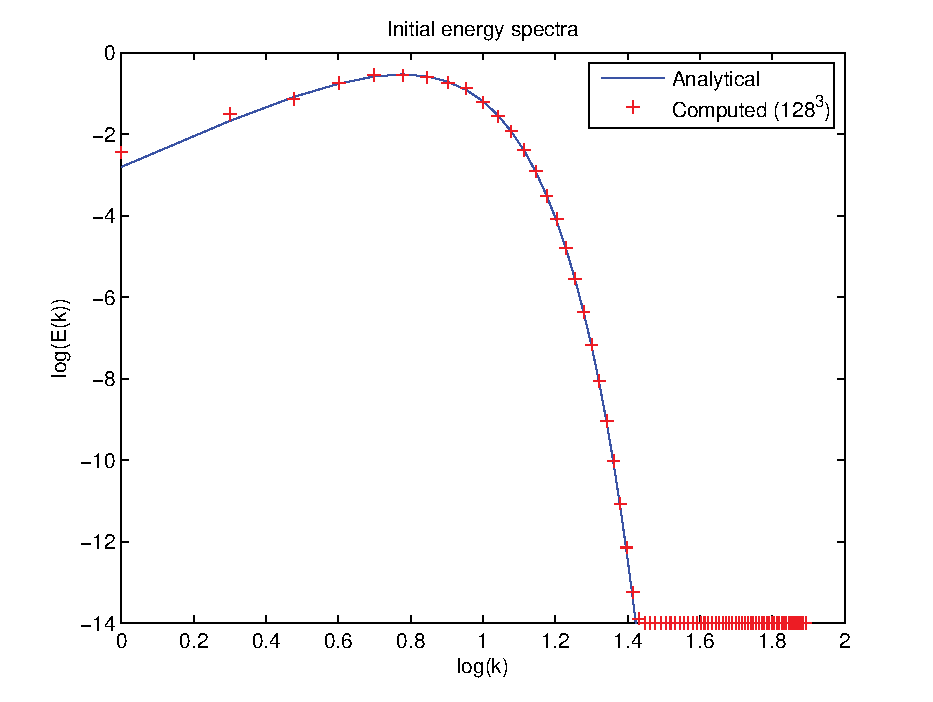
\includegraphics[width=0.6\textwidth]{Figures/Chapter3/DHIT_initial_energy}
	\caption{Analytical and computed initial energy spectrum for the DHIT test.}
	\label{fig-DHIT_initial_spectrum}
\end{figure}

In \Fig{DHIT_isovorticity} we depict the characteristic structures of a fully developed homogeneous and isotropic turbulent flow, plotting the vorticity isosurfaces obtained in the DHIT tes.
\begin{figure}[h!]
	\centering	
	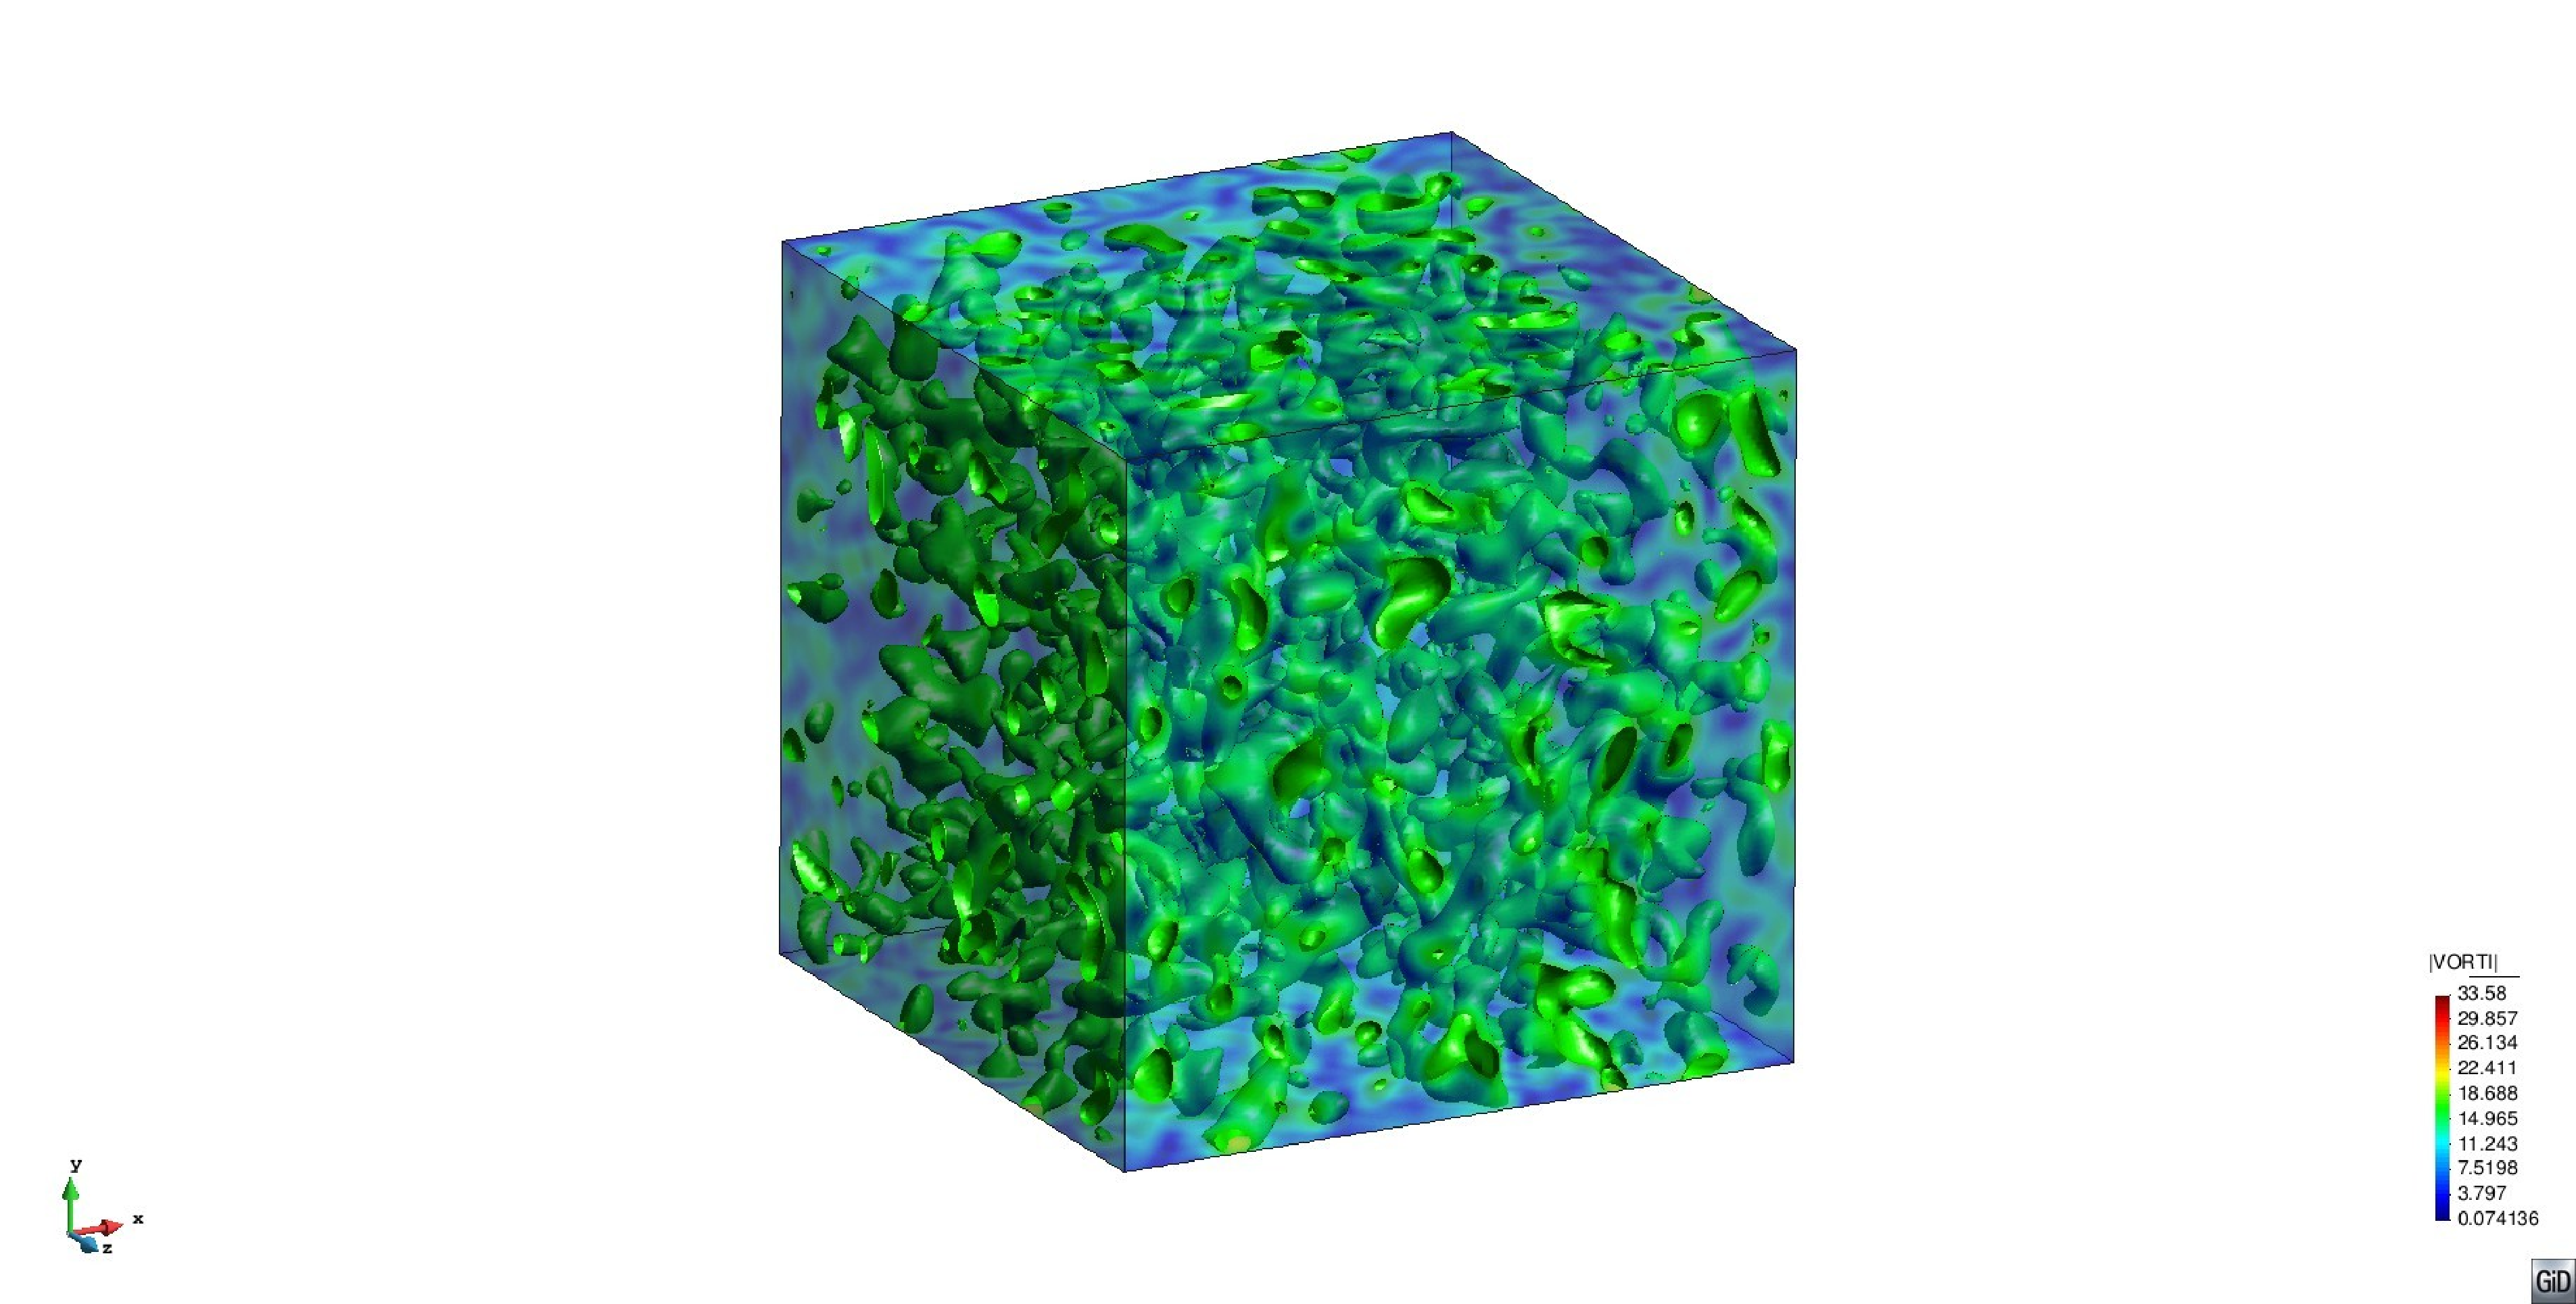
\includegraphics[trim=18cm 3.3cm 14cm 3.2cm,clip=true,width=0.7\textwidth]{Figures/Chapter3/DHIT_isovorticity}
	\caption{Vorticity isosurfaces in the DHIT test.}
	\label{fig-DHIT_isovorticity}
\end{figure}

The initial condition has a relevant role on homogeneous isotropic turbulence. In the final periods of decay, as has been exposed by \cite{hinze_turbulence_1975}, the energy spectrum follows the linear decay law,
\begin{equation}
\label{eq-DHIT_final_decay}
E(k,t)=E(k,0)\exp(-2\nu k^2t).
\end{equation}
So, a first conclusion we can point out from \Eq{DHIT_final_decay} is that the initial spectra, $E(k,0)$, in the final period of decay, has a direct relation with the decay exponent. The total kinetic energy can be calculated integrating \Eq{DHIT_final_decay} over all wave numbers. Then, when $t\rightarrow\infty$, the power law decay is determined by the shape of the initial spectrum.

Moreover, \cite{Staffman 1967} showed that if the initial field is generated by random impulsive forces, a spectrum of the form
\begin{equation}
\label{eq-DHIT_staffman_decay}
E(k,t)\sim k^2\exp(-2\nu k^2t)
\end{equation}
will ensue. Then, the total kinetic energy will decay with the law $K\sim t^{-3/2}$. But, anyway, we will not consider the case of having impulsive forces acting on the flow.

Also in this direction \cite{rohe_analysis_2010} and \cite{chalot_consistent_1998}, say that in the long-run, the energy should decay following the $t^{-1.4}$ law.

\subsubsection{Taylor-Green Vortex flow}
The Taylor-Green Vortex flow (TGV) problem is also a typical and widely used problem on turbulence numerical simulations. First introduced by Taylor and Green (1937) \cite{taylor}, this problem aims to show, in a relatively simple flow, the basic turbulence decay mechanisms like the turbulent energy cascade, the production of small eddies and the enhancement of dissipation by the stretching of vortex lines.

The initial analytical condition for this problem, unlike the DHIT problem, is defined on the physical space. Here we follow \cite{gassner_accuracy_????}, where the initial solution is defined by
\begin{align}
\label{eq-TGV_initial_condition}
&u_x=u_0\cos(x)\sin(y)\sin(z),\\\nonumber
&u_y=-u_0\sin(x)\cos(y)\sin(z),\\\nonumber
&u_z=0,\\\nonumber
&p=p_0+\frac{1}{16}\left(\cos(2x)+\cos(2y)\right)\left(\cos(2z)+2\right).
\end{align}
With
$$u_0=\frac{2}{\sqrt{3}}\sin\left(\gamma+\frac{2\pi}{3}\right).$$
We choose $\gamma=0$, which gives the mean initial velocity  $u_0=1$. The Reynolds number is defined as the inverse of the kinematic viscosity $\nu$, noting that the length and velocity scales are of the same order. This is done according to \cite{gassner_accuracy_????} and \cite{brachet_direct_1991}, and will allow us to compare our results with those showed on these papers. For simplicity, the pressure constant parameter $p_0$ is choosen equal to zero.

With these definitions we can compute analitycaly the initial total kinetic energy of the problem, which is 
\begin{align}
\label{eq-TGV_initial_energy}
K&=\frac{1}{2}\frac{1}{V}\int_0^L\int_0^L\int_0^L\u\cdot\u\ dV\\\nonumber
&=\frac{1}{16\pi^3}\int_0^{2\pi}\int_0^{2\pi}\int_0^{2\pi}\left(u_x^2+u_y^2+u_z^2\right)dxdydz\\\nonumber
&=\frac{u_0^2}{16\pi^3}\int_0^{2\pi}\int_0^{2\pi}\int_0^{2\pi}\left(\cos^2(x)\sin^2(y)+\sin^2(x)\cos^2(y)\right)\sin^2(z)dxdydz\\\nonumber
&=\frac{u_0^2}{8}.
\end{align}

We also can calculate the initial enstrophy of the problem, given by the following expression
\begin{align}
\label{eq-TGV_wnstrophy}
Z&=\frac{1}{2V}\int_0^L\int_0^L\int_0^L\nabla\u:\nabla\u\ dV\\\nonumber
&=\frac{1}{16\pi^3}\int_0^{2\pi}\int_0^{2\pi}\int_0^{2\pi}\left(\sum_{i=1}^3\sum_{j=1}^3\left(\frac{\partial u_i}{\partial x_j}\right)^2\right)dxdydz\\\nonumber
&=\frac{u_0^2}{16\pi^3}\int_0^{2\pi}\int_0^{2\pi}\int_0^{2\pi}\left[2\sin^2(z)\left(\sin^2(x)\sin^2(y)+\cos^2(x)\cos^2(y)\right)\right.\\\nonumber
&+\left.\cos^2(z)\left(\cos^2(x)\sin^2(y)+\sin^2(x)\cos^2(y)\right)\right]dxdydz\\\nonumber
&=\frac{3}{8}u_0^2.
\end{align}

Another interesting result coming from the definition of the initial condition \Eq{TGV_initial_condition} is its representation on the Fourier space. According to Fauconnier et al, \cite{fauconnier_construction_2009}, the initial velocity field on the Fourier space corresponds to eight Fourier modes located at $\mathbf{k}=(\pm1,\pm1,\pm1)$. It means that the initial flow generates a single  vortex scale.

One of the peculiarities about the TGV test is that the initial condition has two-dimensional streamlines, on the $x-y$ plan, but the flow is three dimensional (the initial velocity field also depends on the $z$ direction). 

It is also important to be said that the initial flow is highly symmetric. This symmetry makes that, as stressed by Brachet et al. \cite{brachet_small-scale_1983}, for all times, no fluid crosses any plan such that $x$, $y$ or $z=n\pi$, being $n$ an integer. Taking into account these flow properties we can define the region $0\leq x,y,z\leq\pi$ as the \textit{impermeable box}, since there is a confination of the flow inside this domain. The whole region, $0\leq x,y,z\leq2\pi$, can be called the \textit{periodic box}. Finally, due to the flow symmetries, there is a region from which we can determine the flow at any point in the space. This region is called \textit{fundamental box} and is generated by the box $0\leq x,y,z\leq\frac{1}{2}\pi$.

It can be seen that the perpendicular velocity component, $u_\perp$, and the normal derivative of the parallel velocity component, $\frac{\partial u_\parallel}{\partial n}$, for each impermeable box face vanish on this face. That is, given a face $\Gamma_i$
\begin{align}
\label{eq-TGV_u_perp}
u_\perp|_{\Gamma_i}=0,\quad\mbox{and}\quad\frac{\partial u_\parallel}{\partial n}|_{\Gamma_i}=0.
\end{align}

Equation \Eq{TGV_u_perp} has a direct implication to the voritcity field, $\boldsymbol{\omega}$. For a given impermeable box face, the vorticity on this face can be defined in terms of perpendicular and parallel components as
\begin{align}
\label{eq-TGV_vorticity}
\omega_{\parallel_1}=\left(\frac{\partial u_{\parallel_2}}{\partial x_\perp}-\frac{\partial u_\perp}{\partial x_{\parallel_2}}\right)=0,\\\nonumber
\omega_{\parallel_2}=\left(\frac{\partial u_{\parallel_1}}{\partial x_\perp}-\frac{\partial u_\perp}{\partial x_{\parallel_1}}\right)=0,\\\nonumber
\omega_\perp=\left(\frac{\partial u_{\parallel_1}}{\partial x_{\parallel_2}}-\frac{\partial u_{\parallel_2}}{\partial x_{\parallel_1}}\right)\neq0.
\end{align}
Which means that the vorticity is perpendicular to each impermeable box face.

We solve the Taylor-Green vortex (TG) problem using a Reynolds number $Re=1600$. The most common Reynolds numbers available in the literature are ${\rm Re}=800$, ${\rm Re}=1600$ and ${\rm Re}=3000$ (see, e.g., \cite{andrea_d._beck_numerical_2012, fauconnier_construction_2009, gassner_accuracy_????, jb_chapelier_final_2012}).

The TGV test is characterized by its laminar evolution at the initial time steps, when the flow is strongly anisotropic due to the structured large-scale vortexes directly related to the initial condition. If the Reynolds number is large enough, there appears the vortex-stretching process, which introduce the energy cascade effect, transfering energy from large to small-scales. Because of this procedure, the flow becomes unstable and, therefore, turbulent. According to Brachet et al. \cite{brachet_small-scale_1983}, the flow becomes nearly isotropic for $Re\geq1000$.

In \Fig{TGV_vorticity_streamlines} we depict a vorticity isosurface image computed using a $128^3$ trilinear hexaedral elements mesh. In this picture we can see the symmetry plans stated before.

%\begi\end{figure}d{figure}
\begin{figure}[h!]
	\centering	
	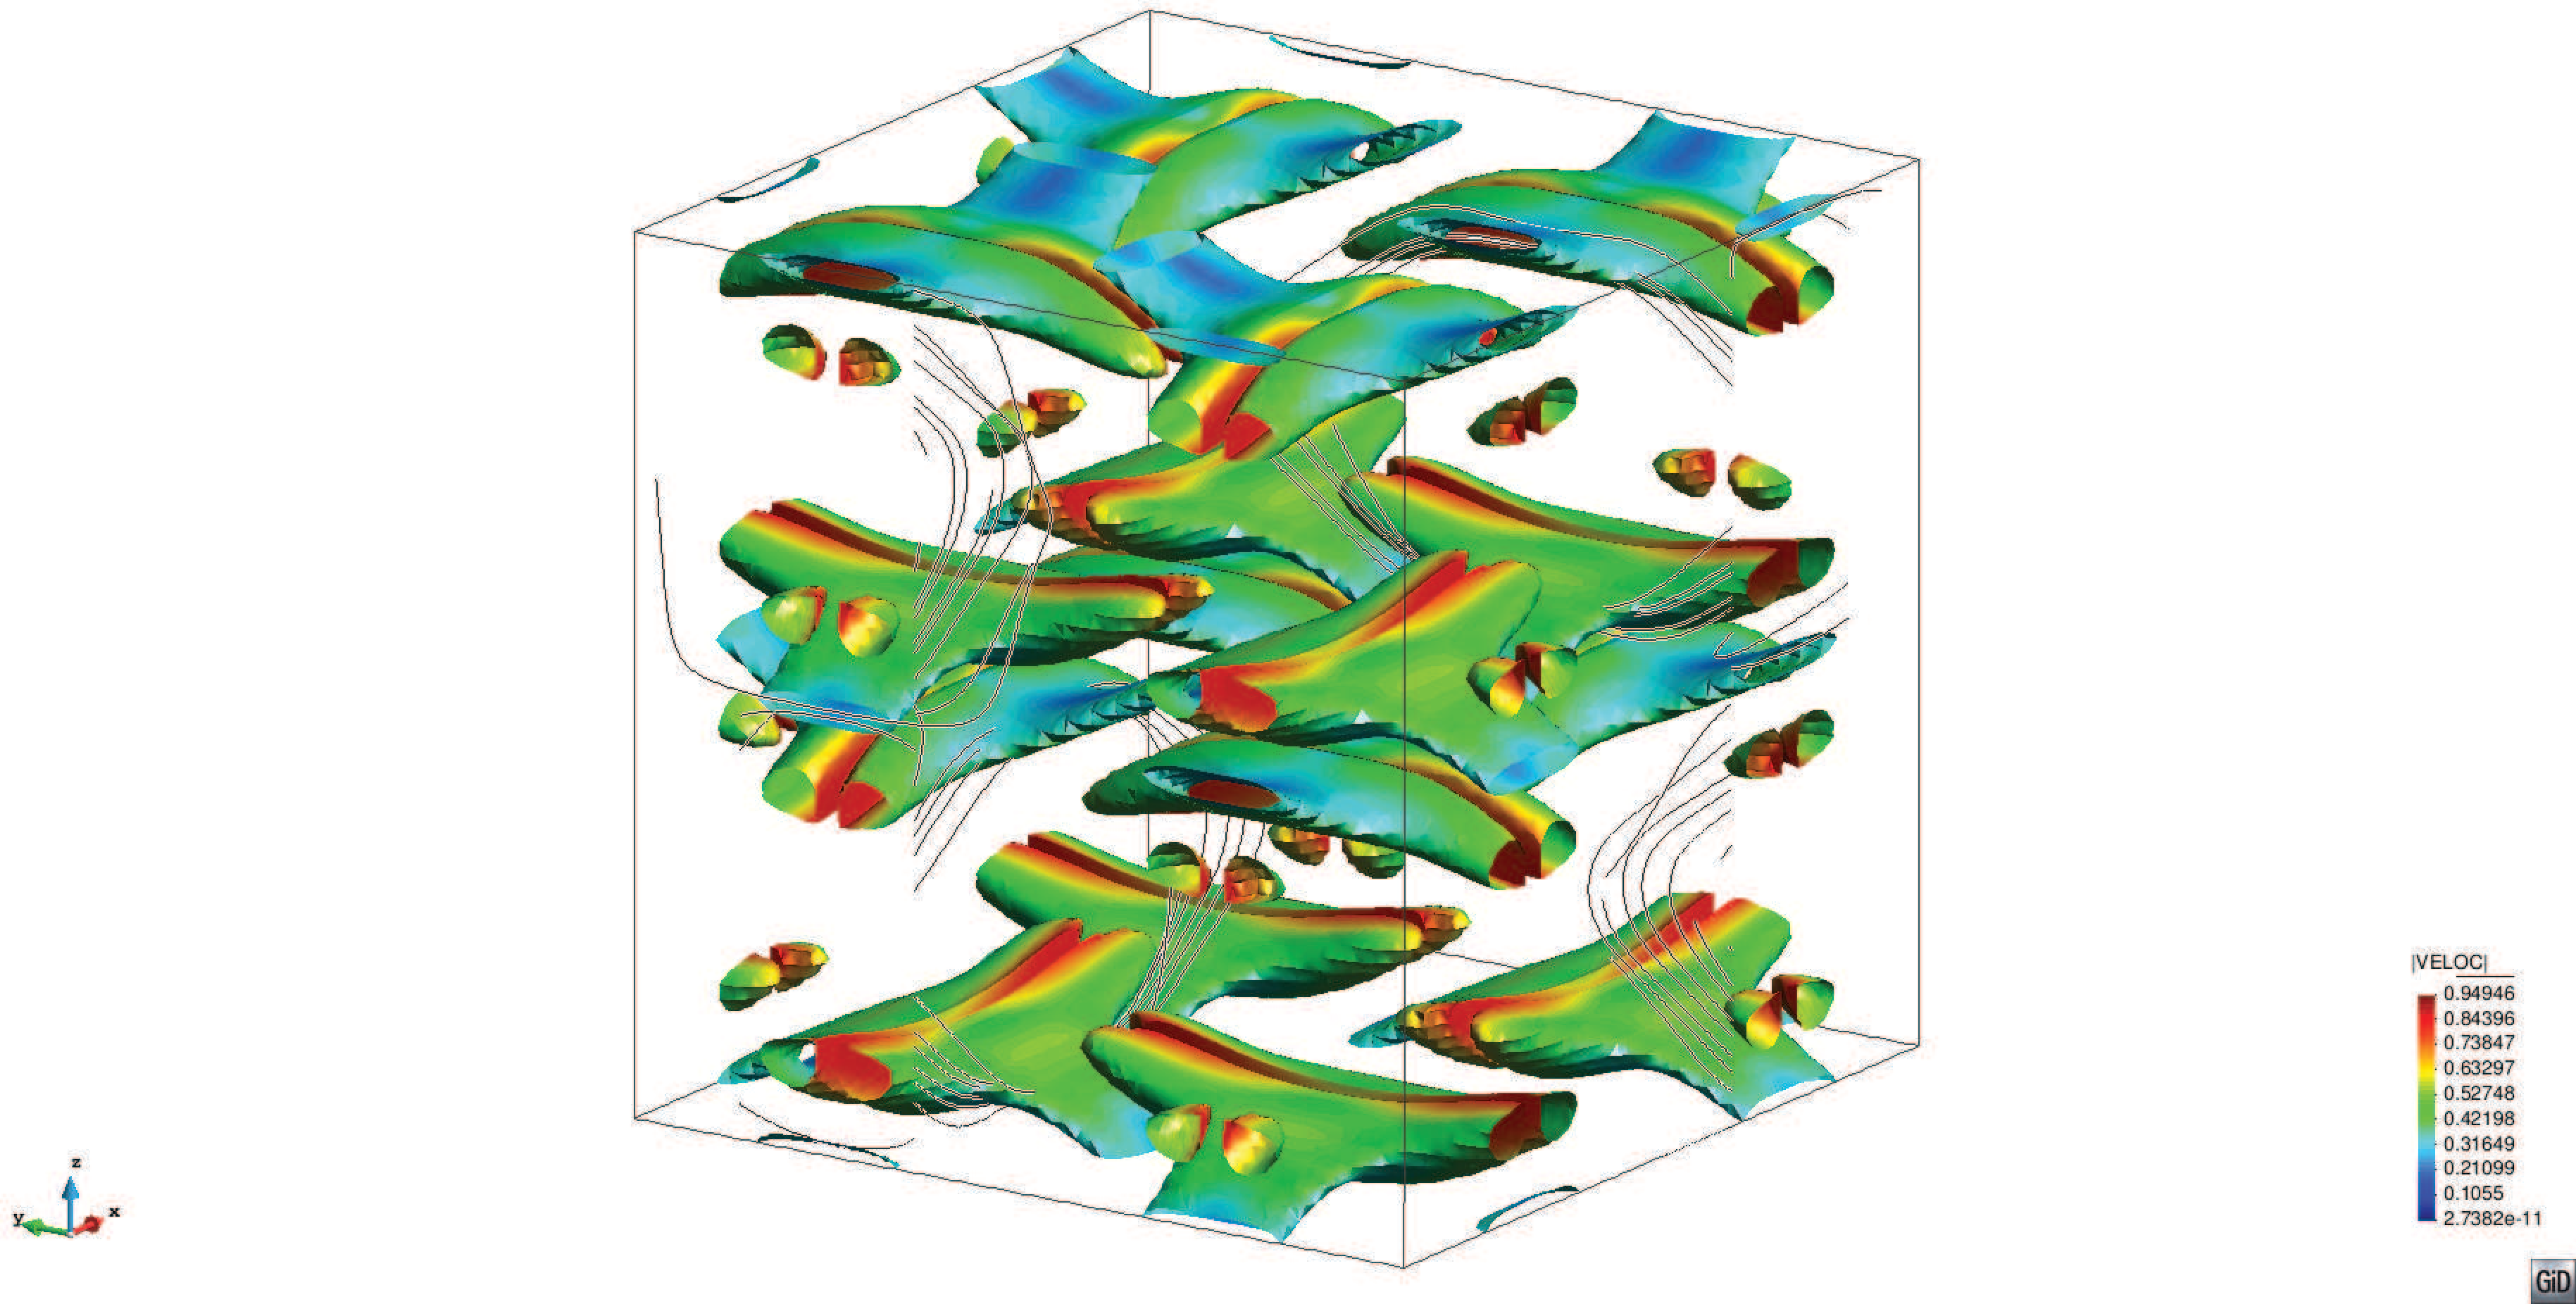
\includegraphics[clip=true, trim=13cm 0cm 13cm 0cm, width=0.6\textwidth]{Figures/Chapter3/TGV_isovorti_streaml_veloc_1}
	\caption{Vorticity isosurfaces at $t=4,0$ with streamlines for the TGV test.}
	\label{fig-TGV_vorticity_streamlines}
\end{figure}

\section{Turbulence in wall-bounded flow}
The vast majority of turbulent flows that we can find in the nature are bounded by, at least, one solid surface. Some examples of bounded flows can be the flow throug a pipe or a duct, the flow in a channel or a river, the flow around an aircraft or a ship, or even the atmospheric flow that is bounded by the terrain. In a turbulent wall-bounded flow, the turbulence is generated through the viscous forces near the wall and then propagated to the outer layer. In this kind of flows, we are interested on defining the mean velocity profiles as well as the friction laws, which will allow us to determine the forces that the fluid flow exerts on the the solid wall.
\subsection{Mean flow}
\subsubsection{Shear stress}
Let us assume that within a certain region near the wall the mean velocity is parallel, or almost parallel, to that wall. We consider that we have a wall on the plane $ (x-z) $ where the mean flow is predominantly in the $ x $-direction, which we will denote as the stream-wise direction and statistically independent of $ z $. The $ y $-direction will be denoted by the wall-normal direction and the $ z $-direction the span-wise direction. Under this assumtions, $ \left\langle u_z\right\rangle=0 $ and the $ \left\langle u_x\right\rangle $ is independent of $ x $, leading to a mean continuity equation
\begin{equation}
\label{eq-mean_continuity}
\frac{d\left\langle u_y\right\rangle}{dy}=0.
\end{equation}

From the mean meomentum equation in the wall-normal direction we can conclude that the pressure is uniform across the flow, satisfying $$ \frac{\partial\left\langle p\right\rangle}{\partial x}=\frac{d p_w}{dx}, $$ being $ p_w(x) $ the pressure value at the wall. Then, from the axial mean momentum equation we have that the shear total shear stress $ \tau(y) $ follows
\begin{equation}
\label{eq-shear_stress_law}
\frac{d\tau}{dy}=\frac{d p_w}{dx},
\end{equation}
with
\begin{equation}
\label{eq-shear_stress}
\tau(y):=\nu\frac{d\left\langle u_x\right\rangle}{dy}-\left\langle u_xu_y\right\rangle,
\end{equation}
see \cite{pope} for a more detailed deduction. We will denote the wall shear stress as $ \tau_w:=\tau(0) $. It is seen that the shear stress is the sum of the viscous stress, $ \nu\frac{d\left\langle u_x\right\rangle}{dy} $, and the Reynolds stress $ -\left\langle u_xu_y\right\rangle $. At the wall, the no-slip boundary condition, $ \u=0 $, implies that
\begin{equation}
\label{eq-wall_shear_stress}
\tau_w=\nu\left.\frac{d\left\langle u_x\right\rangle}{dy}\right|_{y=0}.
\end{equation}

\subsubsection{Friction quantities}
From \Eq{wall_shear_stress} one can observe that the viscosity $ \nu $ is an important parameter in tubulent wall-bounded flows, particularly in the region near the wall. Hence, the mean velocity profile  will depend on the Reynolds number. Moreover, in the region near the wall we can define the appropiate viscous velocity and length scales. We will call friction velocity the velocity scale in the near-wall region, which is defined as
\begin{equation}
\label{eq-friction_velocity}
u_\tau:=\sqrt{\frac{\tau_w}{\rho}},
\end{equation}
and the viscous length scale as 
\begin{equation}
\label{eq-viscous_lenghtscale}
\delta_\nu:=\nu\sqrt{\frac{\rho}{\tau_w}}=\frac{\nu}{u_\tau}.
\end{equation}
Note that the Reynolds number based on the viscous scales is equal to the unity, $ Re_\nu = \frac{u_\tau\delta_\nu}{\nu}=1 $. An alternative is the so called friction Reynolds number, which is defined as
\begin{equation}
\label{eq-friction_reynolds}
Re_\tau:=\frac{u_\tau\delta}{\nu},
\end{equation}
being $ \delta $ the boundary layer thicknes. 

For wall-bounded turbulent flows it is a common practise to use the quantities in terms of wall units. We will define the distance from the wall in wall units as $ y^+:=\frac{y}{\delta_\nu}=\frac{u_\tau y}{\nu} $, and the mean stream-wise velocity in wall units as $ u^+:=\frac{\left\langle u_x\right\rangle}{u_\tau} $.

\subsubsection{Velocity profile}
It has been shown that in the region near the wall, the mean stream-wise velocity can be defined by the distance to the wall. This is known as the law of the wall, which can be expressed in wall units as $ u^+=f_w(y^+) $. In the inner layer, where $ y/\delta\le0.1 $, the law of the wall has been shown to follow the following expression
\begin{equation}
\label{eq-wall_law}
u^+=\frac{1}{\kappa}\ln y^++B,
\end{equation}
whith $ \kappa=0.41 $ and $ B=5.2 $.

\subsection{Turbulent tests}
\subsubsection{Turbulent Channel Flow}
\subsubsection{Turbulent Flow around an airfoil}

\section{Outline and conclusions}

blablabla...

\chapter{Residual-based Variational Multiscale Methods for Large Eddy Simulations}
\label{chap-Rb_VMS}
\section{State of the art}

LES techniques for the numerical simulation of turbulent flows \cite{Sagaut2006} are based on a scale separation that permits to reduce the computational cost with respect to direct numerical simulation (DNS). Such scale separation is traditionally achieved by filtering the original Navier-Stokes equations, which leads to an extra forcing term defined by a physical (functional or structural) model. This widely used approach is usually referred to as explicit LES \cite{Sagaut2006}.

By contrast, implicit LES techniques (ILES) rely on purely numerical artifacts without any modification of the continuous problem. This approach was seldom followed, the MILES (Monotone Integrated LES) approach \cite{Boris1992,Fureby2002,Grinstein2007} being the main exception, until the VMS method was introduced \cite{hughes_multiscale_1995,hughes_variational_1998} and subsequently proposed as an ILES method (see below). ILES techniques are usually considered to be based on the addition of purely dissipative numerical terms, see  \cite[Section 5.3.4]{Sagaut2006}. It is worth to emphasize that this is not the case of some particular VMS models, as it is shown in \cite{Principe2009} and discussed below.

VMS was introduced in \cite{hughes_multiscale_1995,hughes_variational_1998} as a framework for the motivation and development of stabilization techniques, which aim to overcome numerical difficulties encountered when using the standard Galerkin method. On the one hand, the velocity and pressure finite element (FE) spaces need to satisfy the \textit{inf-sup} compatibility condition that guarantees pressure stability and precludes the use of equal order interpolation. Mixed methods satisfying this condition can be used and their finite volume counterpart, based on staggered grids, are common in the LES community. Stabilization techniques that permit the use of equal order interpolation were proposed, e.g., in \cite{Douglas_1989,Hughes_1986_5}. % , and finally recast into the VMS framework. 
On the other hand, global nonphysical oscillations appear in the convection dominated regime, when the mesh is not fine enough, that is, for high mesh Reynolds number flows. The only way to overcome this problem is through the addition of some form of dissipation which was recognized in the early development of stabilized methods \cite{Brooks_1982}. Let us note that  the common practice in the LES community is to rely on the explicit extra term introduced by the physical model using high order approximations of the convective term.
\footnote{It is worth to point out that both problems (convection instability and compatibility conditions) are also present in the \textit{linear} Oseen problem. One of the inconsistencies of an explicit LES approach without a numerical dissipation term is that convection is stabilized by a term that comes from the physical model of the nonlinear Navier Stokes equations and such a term is not present when the linear Oseen problem is considered.} 

The first attempts to perform LES using VMS concepts, presented in \cite{Hughes2000,hughes_large_2001,hughes_multiscale_2001,Koobus2004,john_variants_2008},  were performed introducing explicit subgrid modeling. The VMS models used in these works split resolved scales into large and small, introducing an explicit LES model to account for the small scales stress tensor, e.g., a Smagorinsky-type dissipative term acting on the small scales only. As a result, an important fraction of the degrees of freedom are used for the small resolved scales whereas consistency is retained in the large resolved scales only. 

ILES using a VMS approach with resolved and unresolved subgrid scales (the setting that permits to recover stabilized formulations) was suggested in \cite{codina_stabilized_2002} and performed in \cite{Calo_2004,bazilevs_variational_2007,nogueira_implicit_2010}. Excellent results were first presented in \cite{bazilevs_variational_2007}, but using isogeometric analysis for the space approximation \cite{Hughes_2005a}. Compared to classical LES based on filtering, the VMS approach does not face difficulties associated to inhomogeneous non-commutative filters in wall-bounded flows. Further, it retains numerical consistency in the FE equations and optimal convergence up to the interpolation order whereas, e.g., Smagorinsky models introduce a consistency error of order $h^{4/3}$ (see \cite{Hughes2000,hughes_large_2001,bazilevs_variational_2007}).

Scale separation is achieved in the VMS formalism by a variational projection. The continuous unknown is split into a resolvable FE component and an unresolvable subgrid or subscale component. The action of the subscales onto the FE scales can be approximated in different ways, leading to different VMS models but in all cases these models are {\em residual based} (no eddy viscosity is introduced), which permits to retain consistency. Among the modeling possibilities is the choice of the subscale space, first discussed in \cite{codina_stabilization_2000}, where it was enforced to be $L^2$-orthogonal to the FE space. Another modeling ingredient is the possibility of considering time-dependent subscales and to keep the VMS decomposition in all the nonlinear terms, which was studied in \cite{codina_stabilized_2002,codina_time_2007}. Clear improvements have been observed when using dynamic and fully nonlinear models for the simulation of laminar flows \cite{codina_time_2007, Avila2011}.

%Usually, the unresolved scales in LES methods are modeled by physical based models, see ... But it has been seen that variational multiscale methods (VMS) can reproduce the effect of the small scales in the flow, as it was introduced in Hughes et al. \cite{hughes_large_2001}. Bazilevs et al. in \cite{bazilevs_variational_2007} stress the fact that with this method additional models as eddy viscosities are not needed. 
%The Galerkin FE method used to solve the Navier-Stokes equations for incompressible flows it is known to have some numerical difficulties. For convection dominating problems, which is the case of high Reynolds number flows, the solution using the FE method has numerical inestabilities. There also are compatibility conditions between the velocity and pressure FE spaces that is the \textit{inf-sup} or \textit{LBB} condition. 
%To avoid this numerical drawbacks we use residual-based stabilized FE methods derived from the VMS concept. 

%The VMS method was introduced by Hughes \cite{hughes_multiscale_1995} and basically consists on a separition of scales by a variational projection. The coarse scale is resolved using the FE method while the small scale is modeled and introduced to the coarse scale equations without the need to add any subgrid viscosity. Later, Codina \cite{codina_stabilization_2000,codina_stabilized_2002} introduced the concept of orthogonal subscales where the subscale space is suposed to be orthogonal to the FE space. The time-dependence of the subscales was studied in \cite{codina_time_2007} and it is shown to exhibit better properties in terms of stability and accuracy.

In this chapter we assess implicit VMS models for the numerical simulation of turbulent flows. We refer to the original references for a comprehensive treatment of the assumptions of the formulations and their numerical analysis. Our intention here is to compare the different VMS schemes in terms of quality of the results and computational cost, and discuss some implementation aspects that we find particularly relevant for the simulation of turbulent flows. Our main motivation is to compare the influence of using orthogonal subscales, in order to enrich current comparisons on VMS techniques for large-eddy simulations, such as \cite{gamnitzer_time-dependent_2010}, where only non-projected subscales are considered. We present a detailed numerical experimentation for three well known problems: the decay of homogeneous isotropic turbulence (DHIT), the Taylor-Green vortex (TGV) and the turbulent flow in a channel (TCF), described in Section \ref{chap-Turbulence}. Thus, both unbounded and wall-bounded flows are considered; only wall-bounded tests are performed in \cite{gamnitzer_time-dependent_2010}. Some other differences with respect to \cite{gamnitzer_time-dependent_2010} are: 1) we consider a nonlinear sub-scale equation; 2) we do not include the time step size in the stabilization term; 3) we have analyzed the effect of the skew-symmetric term. 
 
The first implementation aspect we discuss is the treatment of the convective term. As it is well-known, the numerical analysis \cite{Badia2013Convergence,Burman2009,guermond_faedogalerkin_2007} requires a skew-symmetric form of this term in order to avoid any positive contribution to the energy estimates that cannot be properly controlled. The construction of numerical schemes that preserve the skew-symmetry of the convective term at the discrete level has been long studied in the finite difference and finite volume contexts \cite{arakawa_computational_1966, verstappen_symmetry-preserving_2003, gassner_skew-symmetric_2013, trias_symmetry-preserving_2014, del_rey_fernandez_review_2014, svard_review_2014}. However, FE formulations used to perform VMS-based LES use either the conservative form \cite{Hughes2000,Koobus2004,bazilevs_variational_2007,Calderer2013, Calo_2004,gamnitzer_time-dependent_2010,gravemeier_algebraic_2010,masud_variational_2011} or the non-conservative one \cite{john_variants_2008,codina_time_2007,Principe2009}. The approach we follow here is similar to that in \cite{Temam_1984} and is based on a split of the convective term into conservative and non-conservative terms. In the FE (variational) context, this simple approach guarantees the preservation of skew-symmetry at the discrete level. We remark that in the nonlinear VMS models the convective velocity is discontinuous (due to the subscale contribution), which prevents us to use some popular skewsymmetric forms. We also show numerically that a positive energy contribution actually appears if a non skew-symmetric form is used. 

The second point that we address is the use of weighted (by the stabilization parameter) projections and consistent mass matrices when orthogonal subscales are considered. Even though it is cheaper to use non-weighted projections and lumped mass matrices, only the use of consistent projections guarantees exact $L^2$ orthogonality. An alternative is the use of Scott-Zhang projections recently proposed in \cite{Badia2012}, although we do not consider this approach here.

We also discuss the influence of the algorithmic constants of the stabilization parameters in the numerical results. In particular, we show that the choice of the stabilization parameter multiplying the div-div term has a strong influence on the numerical results while it is not essential for stability and convergence of the methods. We further analyze the behavior of the VMS formulation as the time step size is reduced. These two facts are actually related by the way the stabilization parameters are usually defined (see \cite{gamnitzer_time-dependent_2010,Hsu2010}).

Finally, we compare the results obtained using VMS models against those obtained using classical LES based on filtering and the dynamic Smagorinsky closure \cite{fauconnier_construction_2009}, and another implicit LES method, the adaptive local deconvolution presented in \cite{hickel_adaptive_2006}. 
%We do so comparing against other author results for the TGV test, using dynamic Smagorinsky and adaptive local deconvolution methods \cite{fauconnier_construction_2009,hickel_adaptive_2006}.
%We do so using the Galerkin approximation of the Navier Stokes equations with a Taylor-Hood $Q$2/$Q$1 interpolation which satisfies the inf-sup condition, relying on the Smagorinsky term to stabilize convection as it is usually done in the LES community. 

The chapter is organized as follows. In Section \ref{sec-C4_formulation} we present the VMS formulation, how to compute truly orthogonal subscales and the different models we aim at analyzing, whereas in Section \ref{sec-C4_energy} we discuss energy conservation statements and how they are influenced by the choice of the VMS method and the definition of the convective term. Sections \ref{sec-C4_DHIT},  \ref{sec-C4_TGV},  \ref{sec-C4_TCF} are devoted to the numerical approximation of the DHIT, the TGV, and the TCF problems, respectively. Sections \ref{sec-C4_effect_const} and \ref{sec-C4_small_time_step} discuss the effect of the algorithmic constants on the results and the behavior of the different schemes in the small time step limit. Some remarks close the article in Section \ref{sec-C4_conclusions}.

%We will not restrict our atention only in the physical point of view, but we also are interested in the numerical conclusions. For instance, we will evaluate the computational cost of the different methods. Another interesting analysis that has been carried out in this article is the stability for the small time-step limit. Gammitzer et al. \cite{gamnitzer_time-dependent_2010} studied the influence of introducing the dependency of the stabiliztion parameters on the time step, proposed by Bazilevs et al. \cite{bazilevs_variational_2007}, in order to avoid convergence problems at small time-steps.

%Other remarks will be made in the present paper concerning on the importance of a correct formulation of the VMS methods. That will include some analysis on the definition of the nonlinear convective term, the nonlinearity of the advection velocity, the correct definition of the projection when using orthogonal subscales or the importance of the algorithmic constants in the stabilization parameters.

\section{Formulation}
\label{sec-C4_formulation}
\subsection{The Galerkin semi-discrete problem}
%\subsection{Navier-Stokes problem}
\label{subsec-C4_NS_formulation}
In order to improve the readability of this chapter we refresh the Navier-Stokes formulation that was already stated in Chapter \ref{chap-Preliminars}. 

Let $\Omega$ be a bounded domain of $\mathbb{R}^d$, where $d=2,3$ is the number of space dimensions, $\Gamma=\partial\Omega$ its boundary and $[0,T]$ the time interval. The strong form of the incompressible Navier-Stokes problem consists of finding the velocity field $\u$ and the pressure field $p$ such that 
\begin{align}
\label{eq-C4_NS_strong_mome}
\partial_t\u-\nu\Delta\u+\u\cdot\nabla\u+\nabla p&=\f&\mbox{in $\Omega\times(0,T)$,}\\
\label{eq-C4_NS_strong_inc}
\nabla\cdot\u&=0&\mbox{in $\Omega\times(0,T)$,}
\end{align}
with $\f$ the force vector and $\nu$ the kinematic viscosity. 

Equations (\ref{eq-C4_NS_strong_mome})-(\ref{eq-C4_NS_strong_inc}) have to be supplied with appropriate boundary and initial conditions. The boundary $\Gamma$ is divided into the Dirichlet ($\Gamma_D$) and the Neumann ($\Gamma_N$) parts such that $\Gamma_D\cup\Gamma_N=\Gamma$ and $\Gamma_D\cap\Gamma_N=\emptyset$. Then, the boundary and initial conditions can be written as
\begin{align}
\label{eq-C4_NS_strong_Dir}
\u&=\u_g&\mbox{on $\Gamma_D\times(0,T]$,}\\
\label{eq-C4_NS_strong_Neu}
(-p \mathbf{I}+\nu(\nabla\u+\nabla\u^T))\cdot\mathbf{n}&=\mathbf{t}_N&\mbox{on $\Gamma_N\times(0,T]$,}\\
\label{eq-C4_NS_strong_Ini}
\u(\x,0)&=\u_0(\x)&\mbox{in $\Omega\times\{0\}$,}
\end{align}
$\mathbf{n}$ being the unit outward vector normal to $\Gamma$. To simplify the exposition, we will consider $\u_g = {\bf 0}$ and $\Gamma_D = \Gamma$ in what follows.

The weak form of the incompressible Navier-Stokes problem (\ref{eq-C4_NS_strong_mome})-(\ref{eq-C4_NS_strong_Ini}) consists, e.g., in finding $[\u,p]\in {L}^2(0,T;\mathcal{V}_0)\times {\cal D}'(0,T;\mathcal{Q}_0)$ (distributions in time with values in $\mathcal{Q}_0$) such that
\begin{equation}
\label{eq-C4_NS_weak}
(\partial_t\u,\v) + B(\u;[\u,p],[\v,q]) = \left<\f,\v\right> 
\quad\quad\forall\v\in\mathcal{V}_0,\quad\forall q\in\mathcal{Q}_0,
\end{equation}
satisfying the initial condition (\ref{eq-C4_NS_strong_Ini}) in a weak sense. Here $\mathcal{V}_0:={H}_0^1(\Omega)^d$, $\mathcal{Q}_0:=L^2(\Omega)/\mathbb{R}$ and the form $B({\a};[\u,p],(\v,q))$ is defined as 
\begin{equation}
\label{eq-C4_bilinear}
B(\a;[\u,p],[\v,q]):=\nu(\nabla\u,\nabla\v)+b(\a,\u,\v)-(p,\nabla\cdot\v)+(q,\nabla\cdot\u)
\end{equation}
where the trilinear weak form of the convective term $b(\u,\v,\w)$ can be written in the following three equivalent ways
\begin{align}
\label{eq-C4_b_noskew}
&b(\u,\v,\w)=(\u\cdot\nabla\v,\w)&&\mbox{Non conservative},\\
\label{eq-C4_b_skew1}
&b(\u,\v,\mathbf{w})=\frac{1}{2}(\u\cdot\nabla\v,\mathbf{w})-\frac{1}{2}(\v,\u\cdot\nabla\mathbf{w})&&\mbox{Skew-symmetric (type 1)},\\
\label{eq-C4_b_skew2}
&b(\u,\v,\mathbf{w})=(\u\cdot\nabla\v,\mathbf{w})+\frac{1}{2}(\v\cdot\mathbf{w},\nabla\cdot\u)&&\mbox{Skew-symmetric (type 2)}.
\end{align}
This equivalence is lost at the discrete level. The skew-symmetric form (type 2) (\ref{eq-C4_b_skew2}) is very common when numerical analysis are presented \cite{Badia2013Convergence,Burman2009,guermond_faedogalerkin_2007} but the skew-symmetric form (type 2) (\ref{eq-C4_b_skew1}) has important advantages when the first argument is a discontinuous function, as will be shown below.

Let us now consider a FE partition $\mathcal{T}_h$ of the domain $\Omega$ from which we can construct conforming finite dimensional spaces for the velocity $\mathcal{V}_{0,h} \subset \mathcal{V}_0$, and for the pressure $\mathcal{Q}_{0,h}\subset \mathcal{Q}_0$. 

The Galerkin FE approximation of (\ref{eq-C4_NS_weak}) consists in finding $[\u_h,p_h]\in {L}^2(0,T;\mathcal{V}_{0,h})\times {\cal D}'(0,T;\mathcal{Q}_{0,h})$ such that
\begin{equation}
\label{eq-C4_NS_galerkin}
(\partial_t\u_h,\v_h) + B(\u_h;[\u_h,p_h],[\v_h,q_h]) =\left<\f,\v_h\right>
\quad\quad\forall\v_h\in\mathcal{V}_{0,h},\forall q_h\in\mathcal{Q}_{0,h}.
\end{equation}

\subsection{VMS framework}
\label{subsec-C4_VMS_framework}
As it was pointed out in Section \ref{sec-VMS_framework}, the Galerkin FE formulation \Eq{C4_NS_galerkin} suffers from numerical instabilities for high mesh Reynolds number problems, i.e., convection dominated flows. The discrete \textit{inf-sup} condition that must be satisfied by the pair $\mathcal{V}_{0,h} \times\mathcal{Q}_{0,h}$ in order to have a well-posed problem with bounded pressure is also a problem that arise in the Galerkin FE formulation. The VMS method described in Section XXX overcomes these two inestabilities.

After the space splitting into the FE space and the supscale space $\mathcal{V}_0=\mathcal{V}_{0,h}\oplus\widetilde{\mathcal{V}}_0$ and $\mathcal{Q}=\mathcal{Q}_{0,h}\oplus\widetilde{\mathcal{Q}}_0$, where $\widetilde{\mathcal{V}}_0$ and $\widetilde{\mathcal{Q}}_0$ are infinite-dimensional spaces that complete the FE spaces in $\mathcal{V}_0$ and $\mathcal{Q}_0$, respectively. The VMS semi-discrete problem reads: find $[\u_h,p_h]\in {L}^2(0,T;\mathcal{V}_{0,h})\times {\cal D}'(0,T;\mathcal{Q}_{0,h})$ such that
\begin{equation}
\label{eq-C4_NS_discrete}
(\partial_t\u_h,\v_h)+(\partial_t\tilde{\u},\v_h)+B(\a;[\u_h,p_h],[\v_h,q_h])+\left(\tilde{\u},\mathcal{L}_{\a}^*(\v_h,q_h)\right)_h-\left(\tilde{p},\nabla\cdot\v_h\right)=\left<\f,\v_h\right>.
\end{equation}
Where $ \mathcal{L}_{\a}^*(\v_h,q_h) $ is the adjoint operator defined in \Eq{C2_vms_adjoint}. The fine scale problem is approximated by
\begin{align}
\label{eq-C4_velo_sgs}
\partial_t\tilde{\u}+\tau_m^{-1}\tilde{\u}=\mathcal{P}(\R_u),\\
\label{eq-C4_press_sgs}
\tau_c^{-1}\tilde{p}=\mathcal{P}(R_p).
\end{align}
With $ \R_u $ the momentum equation residual \Eq{C2_vms_Ru}, $ R_p $ the continuity equation residual \Eq{C2_vms_Rp}. $ \tau_m $ and $ \tau_c $ are the momentum and continuity equations stabilization parameters, respectively, which definition is given by 
\begin{align}
\label{eq-C4_tau_m}
&\tau_m=\left(\frac{c_1\nu}{h^2}+\frac{c_2|\a|}{h}\right)^{-1},\\
\label{eq-C4_tau_c}
&\tau_c=\frac{h^2}{c_1\tau_m}.
\end{align}

The particular VMS method will result from the combination of the three particular ingredients discussed in Sections \ref{subsec-C2_vms_dyn}-\ref{subsec-C2_vms_oss}, the dynamics of the subscale velocity, the nonlinearity of the advection velocity and the definition of the projection.

\section{Energy balance statements}
\label{sec-C4_energy}

In this section we revisit global energy conservation statements of the method. As shown in \cite{Principe2009}, similar statements can be obtained locally (in a volume $\omega \subset \Omega$).

Taking $\v_h=\u_h$ and $q_h=p_h$ in (\ref{eq-C4_NS_discrete}) we have the energy balance on the FE component
\begin{align}
\label{eq-C4_FE_balance2}
\underbrace{\frac{1}{2}d_t\|\u_h\|^2}_I
& +\underbrace{\nu\|\nabla\u_h\|^2}_{II}
  +\underbrace{b(\a,\u_h,\u_h)}_{III} \\ \nonumber
& +\underbrace{(\partial_t\tilde{\u},\u_h)
+\left(\tilde{\u},\mathcal{L}^*_{\a}(\u_h,p_h)\right)_h
-\left(\tilde{p},\nabla\cdot\u_h\right)}_{IV}
=\underbrace{\left<\mathbf{f},\mathbf{u}_h\right>}_V,
\end{align}
In equation (\ref{eq-C4_FE_balance2}) we group the terms as
% \begin{center}
% \begin{tabular}{rll}
% I)&FE time derivative term:&$\frac{1}{2}d_t\|\u_h\|^2$\\
% II)&FE viscous term:&$\nu\|\nabla\u_h\|^2$\\
% III)&Convective term:&$b(\a,\u_h,\u_h)$\\
% IV)&FE to subscale energy transfer terms:&$(\partial_t\tilde{\u},\u_h)-\left(\tilde{\u},\mathcal{L}^*_{\a}(\u_h,p_h)\right)-\left(\tilde{p},\nabla\cdot\u_h\right)$\\
% V)&FE work of external power:& $\left<\mathbf{f},\mathbf{u}_h\right>$\\
% \end{tabular}
% \end{center}
\begin{center}
\begin{tabular}{rll}
I)&FE kinetic energy variation:&$\frac{1}{2}d_t\|\u_h\|^2$\\
II)&FE viscous dissipation:&$\nu\|\nabla\u_h\|^2$\\
III)&FE convective term:&$b(\a,\u_h,\u_h)$\\
IV)&FE to SGS energy transfer:&$\varepsilon_{h} =(\partial_t\tilde{\u},\u_h)+\left(\tilde{\u},\mathcal{L}^*_{\a}(\u_h,p_h)\right)_h-\left(\tilde{p},\nabla\cdot\u_h\right)$\\
V)&FE component of external power:& $\left<\mathbf{f},\mathbf{u}_h\right>$\\
\end{tabular}
\end{center}
Multiplying (\ref{eq-C4_velo_sgs}) by $\tilde{\u}$ and (\ref{eq-C4_press_sgs}) by $\tilde{p}$, integrating over the domain and decomposing the residual of the momentum equation as $\R_u=\f-\partial_t\u_h-\mathcal{L}_{\a}(\u_h,p_h)$, % we have from (\ref{eq-C4_sgs_balance1}) 
we obtain the global energy balance on the fine scale
\begin{align}
\label{eq-C4_sgs_balance2}
\underbrace{\frac{1}{2}d_t\|\tilde{\u}\|^2}_I
&+\underbrace{\tau_m^{-1}\|\tilde{\u}\|^2}_{II}
+\underbrace{\tau_c^{-1}\|\tilde{p}\|^2}_{III} \\ \nonumber
&+\underbrace{\left(\mathcal{P}(\partial_t\u_h),\tilde{\u}\right)
+\left(\mathcal{P}(\mathcal{L}_{\a}(\u_h,p_h)),\tilde{\u}\right)_h
+\left(\mathcal{P}(\nabla\cdot\u_h),\tilde{p}\right)}_{IV}
=\underbrace{\left(\mathcal{P}(\f),\tilde{\u}\right)}_V.
\end{align}
% In equation (\ref{eq-C4_sgs_balance2}) we group the terms as
% \begin{center}
% \begin{tabular}{rll}
% I)&Subscale time derivative term:&$\frac{1}{2}d_t\|\tilde{\u}\|^2$\\
% II)&Subscale viscous term:&$\tau_m^{-1}\|\tilde{\u}\|^2$\\
% III)&Subscale pressure term:&$\tau_c^{-1}\|\tilde{p}\|^2$\\
% IV)&Subscale to FE energy transfer balance:&$\left(\mathcal{P}(\partial_t\u_h),\tilde{\u}\right)+\left(\tilde{\u},\mathcal{P}(\mathcal{L}_{\a}(\u_h,p_h))\right)+\left(\tilde{p},\mathcal{P}(\nabla\cdot\u_h)\right)$\\
% V)&Subscale work of external power:&$\left(\mathcal{P}(\f),\tilde{\u}\right)$\\
% \end{tabular}
% \end{center}
We group the terms in (\ref{eq-C4_sgs_balance2}) as
\begin{center}
\begin{tabular}{rll}
I)&SGS kinetic energy variation:&$\frac{1}{2}d_t\|\tilde{\u}\|^2$\\
II)&SGS velocity dissipation:&$\tau_m^{-1}\|\tilde{\u}\|^2$\\
III)&SGS pressure dissipation:&$\tau_c^{-1}\|\tilde{p}\|^2$\\
IV)&SGS to FE energy transfer:&$\tilde{\varepsilon}= \left(\mathcal{P}(\partial_t\u_h),\tilde{\u}\right)+\left(\tilde{\u},\mathcal{P}(\mathcal{L}_{\a}(\u_h,p_h))\right)_h+\left(\tilde{p},\mathcal{P}(\nabla\cdot\u_h)\right)$\\
V)&SGS component of external power:&$\left(\mathcal{P}(\f),\tilde{\u}\right)$\\
\end{tabular}
\end{center}
Finally, adding up equations (\ref{eq-C4_FE_balance2}) and (\ref{eq-C4_sgs_balance2}) 
%and using $\mathcal{L}^*(\u_h,p_h)=-\mathcal{L}(\u_h,p_h)$ for linear elements, 
we obtain an equation for the total kinetic energy
\begin{align}
\label{eq-C4_total_balance}
   \frac{1}{2}d_t\|\u_h\|^2
& +\frac{1}{2}d_t\|\tilde{\u}\|^2
  +\nu\|\nabla\u_h\|^2+b(\a,\u_h,\u_h)
  +\tau_m^{-1}\|\tilde{\u}\|^2+\tau_c^{-1}\|\tilde{p}\|^2 \\ \nonumber
& +(\partial_t\tilde{\u},\u_h)
  +\left(\mathcal{P}(\partial_t\u_h),\tilde{\u}\right)
  +\left(\mathcal{P}(\mathcal{L}_{\a}(\u_h,p_h))+\mathcal{L}^*_{\a}(\u_h,p_h),\tilde{\u}\right)_h\\ \nonumber
& \quad \quad \quad \quad  +\left(\mathcal{P}(\nabla\cdot\u_h)-\nabla\cdot\u_h,\tilde{p}\right)=\left<\mathbf{f},\mathbf{u}_h\right>+\left((\mathcal{P}(\f),\tilde{\u}\right).
\end{align}
%Even though it is not our intention to perform a numerical analysis of the methods, let us review known results for each particular VMS model. 
Let us note the presence of $b(\a,\u_h,\u_h)$, which is zero only when the skew-symmetric type 1 form is considered. Other choices could result in a spurious positive contribution to the FE kinetic energy as it is actually observed in the DHIT problem, and could result in a loss of stability, although that was not observed.
%We restric the discussion to the linear version of the multiscale splitting, we are not aware of any result about the fully nonlinear case.

\subsection{Static subscales} 

In this case the energy balance for the subscale is meaningless because there are explicit expressions for the subscales (\ref{eq-C4_static_sgs}) and (\ref{eq-C4_press_sgs}). When (\ref{eq-C4_static_sgs}) and (\ref{eq-C4_press_sgs}) are used in (\ref{eq-C4_FE_balance2}), we obtain
\begin{align}
\label{eq-C4_static_energy}
\frac{1}{2}d_t\|\u_h\|^2
& +\nu\|\nabla\u_h\|^2 + b(\a,\u_h,\u_h)  
  + \left( \tau_{m} \mathcal{P} \left(  \partial_t \u_h \right), \mathcal{L}^*_{\a} ( \u_{h},p_h)\right)_h \\ \nonumber
& + \left(\tau_{m} \mathcal{P} \left( \mathcal{L}_{\a} ( \u_{h},p_h) \right),\mathcal{L}^*_{\a}(\u_h,p_h)\right)_h
%+ \left(\tau_{c} \mathcal{P} (\nabla \cdot \u_{h}),\nabla\cdot\u_h\right)
+ \tau_{c} \left\| \mathcal{P}(\nabla \cdot \u_{h})\right\|^{2}\\ \nonumber
& = \langle\mathbf{f},\mathbf{u}_h\rangle + \left(\tau_m \mathcal{P}(\mathbf{f}),\mathcal{L}^*_{\a}(\u_h,p_h)\right)_h.
\end{align}
In the case of the ASGS method, where $\mathcal{P}:=\mathbf{I}$, the fourth term on the left hand side is a source of problems. One the one hand, it cannot be neglected because it is needed to make the method consistent. On the other hand, it can only be controlled by the dissipation of the time integration scheme and is therefore responsible for the introduction of a restriction on the time step size. As a side problem, it is very inconvenient for an implementation if any explicit (operator splitting) time integration is chosen as it results in a non-symmetric mass matrix. This term is not present if the OSS method is chosen using the projection $\mathcal{P}:=\mathbf{I}-\Pi_h$. Stability of both the fully discrete and the semidiscrete Stokes problem have been proven in \cite{Badia2009a}.

The important term is the fifth one, which permits to control
$ \tau_{m} \left\| \mathcal{P} \left( \mathbf{a}\cdot \mathbf{\nabla u}_{h}+\mathbf{\nabla }p_{h}\right) \right\|^{2} $; the FE part in the OSS formulation is readily controlled using inverse estimates. It therefore provides the essential numerical stability. The last term acts as a penalty on the divergence constraint, adding volumetric diffusion and provides (extra, non-essential) numerical stability.

For the OSS method, it is proved in \cite{guasch-codina-13} that the dissipative structure of the discrete problem has the same statistical behavior in fully developed turbulence than the continuous problem, in the sense that this dissipation has the same estimates as the molecular one. Both dissipations could be made equal by a proper choice of the stabilization parameters in (\ref{eq-C4_tau_m}). This, however, requires a small change in the advection velocity of this expression, which depends on an integral length of the problem. See \cite{guasch-codina-13} for details.

\subsection{Dynamic subscales} 

In this case, the time derivative of both the FE and subgrid components have to be considered and an estimator for the kinetic energy variation of both the FE and subgrid velocity can be obtained. The stability of the subgrid scale velocity can then be used to obtain a stability estimate of the FE component in a norm that includes the convective and pressure terms \cite{codina_time_2007,Badia2009a,Badia2010}.\footnote{However, it should be kept in mind that the numerical solution of the problem is the FE component. There is no reason to add the subscale to the final solution as the approximation is limited by the interpolation order, see \cite[Remark 10]{codina_time_2007}.} Therefore, the numerical dissipation of the method is actually given by the energy transfer $\varepsilon_h$ from the FE to the subscale component. 
Using (\ref{eq-C4_velo_sgs})-(\ref{eq-C4_press_sgs}), we get:
\begin{align}
\label{eq-C4_transfer}
\varepsilon_{h} & = 
  \left( \partial_t\tilde{\u} , \u_h\right) 
- \left( \tau_m \partial_t\tilde{\u} , \mathcal{L}^*_{\a} ( \u_{h},p_h)\right) _h 
- \left( \tau_{m} \mathcal{P} \left(  \partial_t \u_h \right), \mathcal{L}^*_{\a} ( \u_{h},p_h)\right)_h \\ \nonumber
& 
- \left( \tau_{m} \mathcal{P} \left(  \mathcal{L}_{\a} ( \u_{h},p_h) \right), \mathcal{L}^*_{\a} ( \u_{h},p_h) \right)_h
+ \tau_{c} \left\| \mathcal{P} \nabla \cdot \u_{h}\right\|^{2}. %\nonumber
\end{align}
Except from the viscous contribution, the last two terms in (\ref{eq-C4_transfer}) are positive, providing dissipation of the FE energy, but the first three could be negative, providing these models with a mechanism to predict a backward energy transfer, not frequently found in classical LES models \cite{Sagaut2006}. It is justified in \cite{Codina-chap-2011} that even if the first three terms may be negative at a certain time instant, their averaged contribution in a time window greater than the largest period needs to be positive, which is the behavior expected of backscatter from a physical point of view. 

For the ASGS method, i.e., $\mathcal{P}:=\mathbf{I}$, the last term in the left hand side of (\ref{eq-C4_total_balance}) vanishes and the previous one reads
\begin{equation}
\left(\mathcal{L}_{\a}(\u_h,p_h)+\mathcal{L}^*_{\a}(\u_h,p_h),\tilde{\u}\right)_h=
-2 \left(\nu\Delta\u_h,\tilde{\u}\right)_h.
\end{equation}
In turn, the time derivatives of the FE and subscale velocities can be combined as
\begin{align}
\label{eq-C4_time_deriv_ASGS}
\frac{1}{2}d_t\|\u_h\|^2+\frac{1}{2}d_t\|\tilde{\u}\|^2+(\partial_t\tilde{\u},\u_h)+\left(\partial_t\u_h,\tilde{\u}\right)=\frac{1}{2}d_t\|\u_h+\tilde{\u}\|^2
\end{align}
to rewrite (\ref{eq-C4_total_balance}) as
\begin{align}
\label{eq-C4_total_balance_ASGS2}
\frac{1}{2}d_t\|\u_h+\tilde{\u}\|^2
&+\nu\|\nabla\u_h\|^2+b(\a,\u_h,\u_h) \\ \nonumber
&+\tau_m^{-1}\|\tilde{\u}\|^2+\tau_c^{-1}\|\tilde{p}\|^2-2 \left(\nu\Delta\u_h,\tilde{\u}\right)=\left<\mathbf{f},\mathbf{u}_h\right>+\left<\mathbf{f},\tilde{\u}\right>.
\end{align}
From this equation, a stability estimate for $\|\u_h+\tilde{\u}\|$ can be obtained as the last term on the left hand side can be controlled using the second one (see \cite[Remark 4.7]{Badia2009a}).% where this stability is proven for the Stokes problem.

Another important point of (\ref{eq-C4_total_balance_ASGS2}) is that it immediately shows that when the mesh is fine enough, i.e., 
\begin{equation*}
\frac{\left| \mathbf{a}\right| h}{\nu }\ll 1,
\end{equation*}
the dissipation of the total energy depends only on the viscosity. Therefore, the dissipative structure is correctly predicted when a laminar flow is considered or when the discretization is fine enough to resolve all scales of the flow, an important advantage over other LES techniques.

On the other hand, for the OSS method, the FE and subgrid kinetic energy can be summed to obtain the total one
\begin{align}
\label{eq-C4_time_deriv_OSS}
\frac{1}{2}d_t\|\u_h\|^2+\frac{1}{2}d_t\|\tilde{\u}\|^2=\frac{1}{2}d_t\|\u_h+\tilde{\u}\|^2.
\end{align}
since $(\partial_t\tilde{\u},\u_h)=(\partial_t\u_h,\tilde{\u})=0$ as soon as we enforce the subscale to be orthogonal to the FE space. This property also guarantees that%{\color{red} (OJO!! si $\mathcal{P}\left(\partial_t\tilde{\u}\right)+\tau_m^{-1}\tilde{\u}=\mathcal{P}(\R_u)$ esto no se cumple con $\mathcal{P}\equiv\Pi^\bot$ porque $(\mathcal{P}(\partial_t\tilde{\u}),\u_h)=0\Rightarrow(\partial_t\tilde{\u},\u_h)=(\Pi_\tau(\partial_t\tilde{\u}),\u_h)\neq0$. Es asi??)} 
\begin{align}
\label{eq-C4_Pi_tau_sgs}
\left(\Pi_m(\mathcal{L}_{\a}(\u_h,p_h)),\tilde{\u}\right) = 0 \\
\left(\Pi_c(\nabla\cdot\u_h),\tilde{p}\right)=0
\end{align}
which implies that the last term on the left hand side of (\ref{eq-C4_total_balance}) vanishes and that the previous one can be written as
\begin{align}
\left(\mathcal{P}(\mathcal{L}_{\a}(\u_h,p_h))+\mathcal{L}^*_{\a}(\u_h,p_h),\tilde{\u}\right)_h
= \left( (\mathcal{L}_{\a}(\u_h,p_h)+\mathcal{L}^*_{\a}(\u_h,p_h),\tilde{\u}\right)_h
=-2 \left(\nu\Delta\u_h,\tilde{\u}\right)_h
\end{align}
as in the ASGS case. Let us note that the Laplacian term can be eliminated without affecting the convergence properties of the method. 
%It can be justified by replacing the elementwise Laplacian by a discrete Laplacian operator in $\mathcal{L}_{\a}$ (see \cite{Badia2013}). 
% {\color{blue}Note that if the dynamic definition of the subscales is considered, the condition (\ref{eq-C4_Pi_tau_sgs}) is achieved only if we use the modified subscale equation (\ref{eq-C4_velo_sgs_projected}) instead of (\ref{eq-C4_velo_sgs}). Using the definition (\ref{eq-C4_Pi_tau_m}) we have that
% \begin{align}
% \label{eq-C4_Pi_tau_sgs_demo}
% \left(\Pi_m(\mathcal{L}_{\a}(\u_h,p_h)),\tilde{\u}\right) 
% & = \left(\Pi_m(\mathcal{L}_{\a}(\u_h,p_h)),\tau_m\mathcal{P}(\R_u)\right)\\\nonumber
% &  -\left(\Pi_m(\mathcal{L}_{\a}(\u_h,p_h)),\tau_m\mathcal{P}(\partial_t\tilde{\u})\right)\\\nonumber
% & = \left(\Pi_m(\mathcal{L}_{\a}(\u_h,p_h)),\tau_m\R_u\right) 
%   - \left(\Pi_m(\mathcal{L}_{\a}(\u_h,p_h)),\tau_m\Pi_m(\R_u)\right)\\\nonumber
% & - \left(\Pi_m(\mathcal{L}_{\a}(\u_h,p_h)),\tau_m\partial_t\tilde{\u}\right)
%   + \left(\Pi_m(\mathcal{L}_{\a}(\u_h,p_h)),\tau_m\Pi_m(\partial_t\tilde{\u})\right)\\\nonumber
% & = 0.
% \end{align}}
Then, the global energy balance equation (\ref{eq-C4_total_balance}) reads
\begin{align}
\label{eq-C4_total_balance_OSS2}
\frac{1}{2}d_t\|\u_h\|^2+\frac{1}{2}d_t\|\tilde{\u}\|^2
&+\nu\|\nabla\u_h\|^2+b(\a,\u_h,\u_h) \\ \nonumber
&+\tau_m^{-1}\|\tilde{\u}\|^2+\tau_c^{-1}\|\tilde{p}\|^2 %- 2 \left(\nu\Delta\u_h,\tilde{\u}\right)
=\left<\mathbf{f},\mathbf{u}_h\right>+\left(\mathcal{P}(\mathbf{f}),\tilde{\u}\right),
\end{align}
which is exactly (\ref{eq-C4_total_balance_ASGS2}) except for the projection of the force in the last term. Stability and convergence of this formulation have been proved in \cite{Badia2010,Badia2013Convergence}.

\section{Final discrete problem}
\label{sec-C4_discrete}
Applying a time integration algorithm to (\ref{eq-C4_NS_discrete})-(\ref{eq-C4_velo_sgs})-(\ref{eq-C4_press_sgs}) we get the fully discrete problem. The final implementation of the discrete problem is written here considering a Picard linearization of the convective term and the Backward Euler (BE) scheme for the time discretization. It can be straightforwardly modified to consider the Crank-Nicolson time integration scheme; this last scheme is the one used in the numerical examples of Sections \ref{sec-C4_DHIT},  \ref{sec-C4_TGV} and \ref{sec-C4_TCF}.

\subsection{Algebraic Subgrid Scales (ASGS)}

Taking the nonlinear advection velocity definition (\ref{eq-C4_a_nl}) and considering the time derivative in the fine scales, we have the Dynamic and Nonlinear ASGS method, hereinafter Dyn-Nl-ASGS. 
%For this method, using linear FEs, the Backward Euler (BE) scheme for the time discretization and the Picard method for the nonlinear term, 
At time step $n$ and nonlinear iteration $i$, given $\u_h^{n,i-1}$, $\u_h^{n-1}$, $\tilde{\u}^{n,i-1}$ and $\tilde{\u}^{n-1}$ we compute $\mathbf{u}_h^{n,i}$ and $ p_h^{n,i} $ such that
% \begin{align}
% \label{eq-C4_Dyn-Nl-ASGS}
% &\frac{1}{\Delta t}(\u_h^{n+1,i},\v_h)+\nu(\nabla\u_h^{n+1,i},\nabla\v_h)+b(\a^{n+1,i-1},\u_h^{n+1,i},\v_h)-(p_h^{n+1},\nabla\cdot\v_h)+(q_h,\nabla\cdot\u_h^{n+1,i})+\\\nonumber
% &+\left(\tau_{m,t}\left[\frac{1}{\Delta t}\u_h^{n+1,i}+N(\a^{n+1,i-1},\u_h^{n+1,i})+\nabla p_h^{n+1}\right],N(\a^{n+1,i-1},\v_h)+\nabla q_h\right)+\\\nonumber
% &+\left(\tau_c\nabla\cdot\u_h^{n+1,i},\nabla\cdot\v_h\right)-\frac{1}{\Delta t}\left(\tau_{m,t}\left[\frac{1}{\Delta t}\u_h^{n+1,i}+N(\a^{n+1,i-1},\u_h^{n+1,i})+\nabla p_h^{n+1}\right],\v_h\right)=\\\nonumber
% &=\langle\v_h,\mathbf{f}\rangle+\frac{1}{\Delta t}(\u_h^{n},\v_h)+\frac{1}{\Delta t}(\tilde{\u}^{n},\v_h)+\left(\tau_{m,t}\left[\frac{1}{\Delta t}\u_h^{n}+\mathbf{f}+\frac{1}{\Delta t}\tilde{\u}^n\right],N(\a^{n+1,i-1},\v_h)+\nabla q_h\right)-\\\nonumber
% &-\frac{1}{\Delta t}\left(\tau_{m,t}\left[\frac{1}{\Delta t}\u_h^{n}+\mathbf{f}+\frac{1}{\Delta t}\tilde{\u}^n\right],\v_h\right),\\\nonumber
% \end{align}
\begin{align}
\label{eq-C4_Dyn-Nl-ASGS}
\frac{1}{\delta t}(\u_h^{n,i},\v_h)
&+ B(\a^{n,i-1};[\u_h^{n,i},p_h^{n,i}],[\v_h,q_h])
\\ \nonumber
&+\left(\tau_{m,t} \left[\frac{1}{\delta t}\u_h^{n,i}+ \mathcal{L}_{\a^{n,i-1}}(\u_h^{n,i},p_h^{n,i})\right], \mathcal{L}^*_{\a^{n,i-1}}(\v_h,q_h) \right)_h\\ \nonumber
&+\left(\tau_c\nabla\cdot\u_h^{n,i},\nabla\cdot\v_h\right)
-\frac{1}{\delta t} \left(\tau_{m,t}\left[\frac{1}{\delta t}\u_h^{n,i}+ \mathcal{L}_{\a^{n,i-1}}(\u_h^{n,i},p_h^{n,i})\right],\v_h\right)_h \\\nonumber
&=\langle\v_h,\mathbf{f}\rangle
+\frac{1}{\delta t}(\u_h^{n-1},\v_h)+\frac{1}{\delta t}(\tilde{\u}^{n-1},\v_h) \\\nonumber
&-\frac{1}{\delta t}\left(\tau_{m,t}\left[\frac{1}{\delta t}\u_h^{n-1}+\mathbf{f}+\frac{1}{\delta t}\tilde{\u}^{n-1}\right],\v_h\right) \\\nonumber
&+\left(\tau_{m,t}\left[\frac{1}{\delta t}\u_h^{n-1}+\mathbf{f}+\frac{1}{\delta t}\tilde{\u}^{n-1}\right],\mathcal{L}^*_{\a^{n,i-1}}(\v_h,q_h) \right)_h,
\label{eq-C4_Dyn-Nl-ASGS}
\end{align}
where $\tau_{m,t}=\left(\delta t^{-1}+\tau_m^{-1}\right)^{-1}$ and $\a^{n,i-1}=\u_h^{n,i-1}+\tilde{\u}^{n,i-1}$.

In turn, $\tilde{\u}^{n,i}$ is computed by solving the discretization of the fine scale problem (\ref{eq-C4_velo_sgs}). Note that in the nonlinear version of the algorithm, the stabilization parameter $\tau_{m,t}$ depends on the subscale itself through $\a$ in (\ref{eq-C4_tau_m}), making the fine scale equation also nonlinear, although it is local and does not increase the size of the global linear system to be solved. At each integration point of each element we iteratively solve
\begin{equation}
\label{eq-C4_velo_sgs_discrete_expl}
\tilde{\mathbf{u}}^{n,i,k}=\tau_{m,t}^{k-1}\frac{1}{\delta t}\tilde{\mathbf{u}}^{n-1}
+ \tau_{m,t}^{k-1} \left[\mathbf{f} - \frac{(\u_h^{n,i}-\u_h^{n-1})}{\delta t} - \mathcal{L}_{\a^{n,i,k-1}}(\u_h^{n,i},p_h^{n,i})\right].
%\left(\frac{(\u_h^{n+1,i}-\u_h^n)}{\Delta t}+N(\a^{n+1,i,k-1},\u_h^{n+1,i})+\nabla p_h^{n+1}\right)\right].
\end{equation}
where $\a^{n,i,k-1}=\u_h^{n,i}+\tilde{\u}^{n,i,k-1}$  is used in (\ref{eq-C4_tau_m}) to obtain $\tau_{m,t}^{k-1}$. 
%We can see that in the equation (\ref{eq-C4_Dyn-Nl-ASGS}) appears an extra variable, $\tilde{\u}$. Then, for the last method we need to compute the fine scale velocity at each nonlinear iteration. But is a local unknown and does not increase the age of the resulting linear system. Note that we need the subscale velocity at the previous time-step, $\tilde{\u}^n$, but also at the previous nonlinear iteration of the current step, $\tilde{\u}^{n+1,i-1}$, needed in $\a^{n+1,i-1}$. This extra variable is obtained by solving the discrete fine scale problem
% \begin{equation}
% \label{eq-C4_velo_sgs_discrete_expl}
% \tilde{\mathbf{u}}^{n+1,i,k}=\tau_{m,t}^{k-1}\frac{1}{\Delta t}\tilde{\mathbf{u}}^n+\tau_{m,t}^{k-1}\left[\mathbf{f}-\left(\frac{(\u_h^{n+1,i}-\u_h^n)}{\Delta t}+N(\a^{n+1,i,k-1},\u_h^{n+1,i})+\nabla p_h^{n+1}\right)\right].
% \end{equation}

%We can observe in equation (\ref{eq-C4_velo_sgs_discrete_expl}) that the fine scale velocity $\tilde{\u}$ is also nonlinear since the stabilization parameter $\tau_{m,t}$ and the advection velocity $\a$ depend on $\tilde{\u}$.
% TILL HERE
 Alternatively, one can send the corresponding fine scale convective term $\tilde{\u}\cdot\nabla\u_h$ to the left-hand side, improving the convergence of the iterative process as
\begin{align}
\label{eq-C4_velo_sgs_discrete_impl}
\tilde{\mathbf{u}}^{n,i,k}
& + \tilde{\u}^{n,i,k}\cdot\nabla\u_h^{n,i}
  = \tau_{m,t}^{k-1} \frac{1}{\delta t} \tilde{\mathbf{u}}^{n-1} + \tau_{m,t}^{k-1} \left[\mathbf{f} - \frac{(\u_h^{n,i}-\u_h^{n-1})}{\delta t} - \mathcal{L}_{\u_h^{n,i}}(\u_h^{n,i},p_h^{n,i})\right].
%& + \tau_{m,t}^{k-1} \left[\mathbf{f}-\left(\frac{(\u_h^{n+1,i}-\u_h^n)}{\Delta t}+N(\u_h^{n+1,i},\u_h^{n+1,i})+\nabla p_h^{n+1}\right)\right].
\end{align}
This is a simple fixed-point iterative scheme that we have found efficient and robust for the numerical simulations presented in this paper, although in other situations we have found more convenient to use a conventional Newton-Raphson scheme to solve the nonlinear subscale equation \cite{Avila2011}.

For the simplest ASGS scheme we do not consider the time derivative of the fine scale, we consider them quasi-static, i.e., $(\partial_t\tilde{\u},\v_h)=0$. Note that in any case the subscales will depend on time through the FE residual and the stabilization parameter. On the other hand, the advection velocity is considered to be linear as indicated in (\ref{eq-C4_a_lin}). We label this method as Static Linear ASGS (Sta-Lin-ASGS). Note that the Sta-Lin-ASGS method does not need to explicitly compute $\tilde{\u}$; invoking (\ref{eq-C4_tau_m}) and (\ref{eq-C4_tau_c}) in (\ref{eq-C4_NS_discrete}) we get a discrete equation only in terms of the FE component.%, avoiding to solve (\ref{eq-C4_velo_sgs_discrete_impl}).

We can readily define the rest of possible combinations of time and nonlinear treatment considering the linear advection velocity definition and the time-dependence in the subscales (Dyn-Lin-ASGS method) or keeping the static definition of the subscales with the nonlinear choice for the advection velocity (Sta-Nl-ASGS method).

\subsection{Orthogonal Subscales (OSS)}

Let us state the Dynamic and Nonlinear OSS (Dyn-Nl-OSS) method, which means to take into account the nonlinearity of the advection velocity (\ref{eq-C4_a_nl}) and the time derivative of the subscales. At time step $n$ and nonlinear iteration $i$, given $\u_h^{n,i-1}$, $\u_h^{n-1}$, $\tilde{\u}^{n,i-1}$ and $\tilde{\u}^{n-1}$ we compute $\mathbf{u}_h^{n,i}$ and $ p_h^{n,i} $ by solving
%problem using linear FEs, a BE discretization in time and the Picard method for the nonlinear term, at time step $t_{n+1}$ and nonlinear iteration $i$, is the following
% \begin{align}
% \label{eq-C4_Dyn-Nl-OSS}
% &\frac{1}{\Delta t}(\u_h^{n+1,i},\v_h)+\nu(\nabla\u_h^{n+1,i},\nabla\v_h)+b(\a^{n+1,i-1},\u_h^{n+1,i},\v_h)-(p_h^{n+1},\nabla\cdot\v_h)+(q_h,\nabla\cdot\u_h^{n+1,i})+\\\nonumber
% &+\left(\tau_{m,t}\left[N(\a^{n+1,i-1},\u_h^{n+1,i})+\nabla p_h^{n+1}\right],N(\a^{n+1,i-1},\v_h)+\nabla q_h\right)+\\\nonumber
% &+\left(\tau_c\nabla\cdot\u_h^{n+1,i},\nabla\cdot\v_h\right)=\langle\v_h,\mathbf{f}\rangle+\frac{1}{\Delta t}(\u_h^{n},\v_h)+\left(\tau_{m,t}\left[\mathbf{f}+\frac{1}{\Delta t}\tilde{\u}^{n}\right],N(\a^{n+1,i-1},\v_h)+\nabla q_h\right)-\\\nonumber
% &-\left(\tau_{m,t}\Pi_m(\R_u^{n+1,i-1}),N(\a^{n+1,i-1},\v_h)+\nabla q_h\right)-\left(\tau_c\Pi_c\left(R_p^{n+1,i-1}\right),\nabla\cdot\v_h\right).\\\nonumber
% \end{align}
\begin{align}
\label{eq-C4_Dyn-Nl-OSS}
\frac{1}{\delta t}(\u_h^{n,i},\v_h)
&+ B(\a^{n,i-1};[\u_h^{n,i},p_h^{n,i}],[\v_h,q_h]) \\ \nonumber
&+\left(\tau_{m,t} \left[\frac{1}{\delta t}\u_h^{n,i}+ \mathcal{L}_{\a^{n,i-1}}(\u_h^{n,i},p_h^{n,i})\right], \mathcal{L}^*_{\a^{n,i-1}}(\v_h,q_h) \right)\\ \nonumber
 &+\left(\tau_c\nabla\cdot\u_h^{n,i},\nabla\cdot\v_h\right) \\\nonumber
 &=\langle\v_h,\mathbf{f}\rangle
 +\frac{1}{\delta t}(\u_h^{n-1},\v_h) \\\nonumber
 &+\left(\tau_{m,t}\left[\mathbf{f}+\frac{1}{\delta t}\tilde{\u}^{n-1}-\boldsymbol{\xi}_m^{n,i-1}\right],\mathcal{L}^*_{\a^{n,i-1}}(\v_h,q_h) \right) \\\nonumber
 &-\left(\tau_c\xi_c^{n,i-1},\nabla\cdot\v_h\right),
\end{align}
% \begin{align}
% \label{eq-C4_Dyn-Nl-OSS}
% &\frac{1}{\Delta t}(\u_h^{n+1,i},\v_h)+\nu(\nabla\u_h^{n+1,i},\nabla\v_h)+b(\a^{n+1,i-1},\u_h^{n+1,i},\v_h)-(p_h^{n+1},\nabla\cdot\v_h)+(q_h,\nabla\cdot\u_h^{n+1,i})+\\\nonumber
% &+\left(\tau_{m,t}\left[N(\a^{n+1,i-1},\u_h^{n+1,i})+\nabla p_h^{n+1}\right],N(\a^{n+1,i-1},\v_h)+\nabla q_h\right)+\\\nonumber
% &+\left(\tau_c\nabla\cdot\u_h^{n+1,i},\nabla\cdot\v_h\right)=\langle\v_h,\mathbf{f}\rangle+\frac{1}{\Delta t}(\u_h^{n},\v_h)+\left(\tau_{m,t}\left[\mathbf{f}+\frac{1}{\Delta t}\tilde{\u}^{n}\right],N(\a^{n+1,i-1},\v_h)+\nabla q_h\right)-\\\nonumber
% &-\left(\tau_{m,t}\Pi_m(\R_u^{n+1,i-1}),N(\a^{n+1,i-1},\v_h)+\nabla q_h\right)-\left(\tau_c\Pi_c\left(R_p^{n+1,i-1}\right),\nabla\cdot\v_h\right).\\\nonumber
% \end{align}
%Here we need to have explicitly defined the projections of the residuals, $\Pi_m(\R_u)$ and $\Pi_c(R_p)$. The implementation on the code of the projection calculations can be done implicitly at each nonlinear iteration ($\Pi_m(\R_u^{n+1,i-1})$ and $\Pi_c(R_p^{n+1,i-1})$), or explicitly at the previous time step ($\Pi_m(\R_u^n)$ and $\Pi_c(R_p^n)$). 
where $\boldsymbol{\xi}_m$ and $\xi_c$ are the weighted projections of the residuals $\R_u$ and $R_p$ (see below) evaluated at the corresponding time step and nonlinear iteration. 

Like the Dyn-NL-ASGS method, we also need to compute the subscale velocity $\tilde{\u}$ explicitly. We compute the discrete subscale problem with the OSS counterpart of (\ref{eq-C4_velo_sgs_discrete_expl}) or (\ref{eq-C4_velo_sgs_discrete_impl}), viz. 
% \begin{align}
% \label{eq-C4_velo_sgs_discrete_impl_OSS}
% \tilde{\mathbf{u}}^{n+1,i,k}
% & + N(\tilde{\u}^{n+1,i,k},\u_h^{n+1,i})=
% \tau_{m,t}^{k-1}\frac{1}{\Delta t}\tilde{\mathbf{u}}^n \\ \nonumber
% & + \tau_{m,t}^{k-1}\left[\mathbf{f}-\left(N(\u_h^{n+1,i},\u_h^{n+1,i})+\nabla p_h^{n+1}\right)\right]-\tau_{m,t}^{k-1}\Pi_m(\R_u^{n+1,i-1}).
% \end{align}
\begin{align}
\label{eq-C4_velo_sgs_discrete_impl_OSS}
\tilde{\mathbf{u}}^{n,i,k}
& + \tilde{\u}^{n,i,k}\cdot\nabla\u_h^{n,i}
  = \tau_{m,t}^{k-1} \frac{1}{\delta t} \tilde{\mathbf{u}}^{n-1} \\ \nonumber
& + \tau_{m,t}^{k-1} \left[\mathbf{f} - \frac{(\u_h^{n,i}-\u_h^{n-1})}{\delta t} - \mathcal{L}_{\u_h^{n,i}}(\u_h^{n,i},p_h^{n,i})\right]-\tau_{m,t}^{k-1}\boldsymbol{\xi}_m^{n,i-1}.
%& + \tau_{m,t}^{k-1} \left[\mathbf{f}-\left(\frac{(\u_h^{n+1,i}-\u_h^n)}{\Delta t}+N(\u_h^{n+1,i},\u_h^{n+1,i})+\nabla p_h^{n+1}\right)\right].
\end{align}
Note that $\boldsymbol{\xi}_m^{n,i}$ actually depends on $\tilde{\u}^{n,i}$ via the advection velocity of the convective term $\a^{n,i}=\u_h^{n,i}+\tilde{\u}^{n,i}$. In order to simplify the fine scale computation (\ref{eq-C4_velo_sgs_discrete_impl_OSS}) we use the projection at the previous nonlinear iteration, i.e., $\boldsymbol{\xi}_m^{n,i-1}$. 

For the dynamic OSS case we should introduce some modifications in the computation of the projection $\Pi_m$. At the fully discrete level, in order for $\tilde{\u}^{n+1}$ to be $L^2$ orthogonal to $\mathcal{V}_{h}$, we must add to the FE residual the subscale time derivative contribution from the previous time step and use $\tau_{m,t}$ instead of $\tau_m$ in the computation of the projections. Finally, the projections of the residuals onto the FE spaces $\boldsymbol{\xi}_m^{n,i}$ and $\xi_c^{n,i}$ are such that
\begin{align}
\label{eq-C4_dyn_proj}
&(\tau_{m,t}\boldsymbol{\xi}_m^{n,i},\v_h)=(\tau_{m,t}(\R_u^{n,i}+\frac{1}{\delta t} \tilde{\mathbf{u}}^{n-1}),\v_h)&&\forall\v_h\in\mathcal{V}_{0,h},\\
&(\tau_c\xi_c^{n,i},q_h)=(\tau_c R_p^{n,i},q_h)&&\forall q_h\in\mathcal{Q}_{0,h},
\end{align}
%\begin{align}
%&(\tau_{m,t}\boldsymbol{\xi}_m^{n,i},\v_h)=(\tau_{m,t} \R_u^{n,i},\v_h)&&\forall\v_h\in\mathcal{V}_{0,h},\\
%&(\tau_c\xi_c^{n,i},q_h)=(\tau_c R_p^{n,i},q_h)&&\forall q_h\in\mathcal{Q}_{0,h}.
%\end{align}
where the residuals $\R_u^{n,i}$ and $R_p^{n,i}$ are evaluated using (\ref{eq-C4_Ru}) and (\ref{eq-C4_Rp}) with $\a^{n,i}=\u_h^{n,i}+\tilde{\u}^{n,i}$, $\u_h^{n,i}$, $\u_h^{n-1}$ and $p_h^{n,i}$. %It is also possible to compute projections explicitly, using the residuals evaluated with $\a^{n-1}=\u_h^{n-1}+\tilde{\u}^{n-1}$, $\u_h^{n-1}$, $\u_h^{n-2}$ and $p_h^{n-1}$ but we do not use this option here.  
 Note that when convergence of the nonlinear iteration is achieved, (\ref{eq-C4_velo_sgs_discrete_impl_OSS}) and (\ref{eq-C4_dyn_proj}) guarantee that $(\v_h,\tilde{\mathbf{u}}^{n}) = 0$ for any $\v_h\in\mathcal{V}_{0,h}$.

\section{Numerical experiments}
\subsection{Decay of homogeneous isotropic turbulence}
\label{subsec-C4_DHIT}
This problem, one of the most used benchmarks to test LES models, consists of analyzing the statistics of the turbulent flow in a 3D box of size $\Omega=(0,2\pi)\times(0,2\pi)\times(0,2\pi)$ with periodic boundary conditions in all directions, which is started with a field having a predetermined energy spectrum. A detailed description of the computational domain, initial conditions, and problem setting is given in \cite{mansour_decay_1994}. Furthermore, the main characteristics of this test are stated in Section \ref{subsec-DHIT}.,

We recall that the initial energy spectra is:
\begin{equation}
\label{eq-C4_ini_E_DHIT2}
E(k,0)=16\sqrt{\frac{2}{\pi}}k_0^{-5}k^4\exp\left(-2\left(\frac{k}{k_0}\right)^2\right).
\end{equation}
The initial energy spectrum defined in (\ref{eq-C4_ini_E_DHIT2}) has a peak on the wavenumber $k_0=6$ which supposes that the total kinetic energy at the initial time step should be $1/2q^2=1.5$ and the enstrophy $\frac{1}{2}<w^2>=67.5$.

\subsubsection{Setting}
\label{subsubsec-C4_DHIT_setting}
We solve the DHIT test using different meshes ($32^3$, $64^3$ and $128^3$ $Q_1/Q_1$ elements). 

%In what concerns on the tested VMS methods, we use 
We test the ASGS method and the OSS method reported in Section \ref{sec-C4_discrete}. The problem is solved considering three different cases for both methods, depending on the definition of the advection velocity and the tracking of the subscales. The advection velocity $\a$ can be linear or nonlinear and the subscales can be dynamic or static (see Subsection \ref{subsec-C4_VMS_framework}). Table \ref{table:DHIT_cases} collects all the VMS combinations to be compared for the different simulations.

\begin{table}[h]
\centering
\begin{tabular}{ccccc}
\hline
Case Id.&Label&Method&Advection velocity ($\a$)&Subscales tracking\\
\hline
1&Sta-Lin-ASGS&ASGS&Linear ($\a=\u_h$)&Static ($\partial_t\tilde{\u} = {\bf 0}$)\\
2&Dyn-Lin-ASGS&ASGS&Linear ($\a=\u_h$)&Dynamic ($\partial_t\tilde{\u} \not = {\bf 0}$)\\
3&Dyn-Nl-ASGS&ASGS&Nonlinear ($\a=\u_h+\tilde{\u}$)&Dynamic ($\partial_t\tilde{\u} \not = {\bf 0}$)\\
\hline
4&Sta-Lin-OSS&OSS&Linear ($\a=\u_h$)&Static ($\partial_t\tilde{\u} = {\bf 0}$)\\
5&Dyn-Lin-OSS&OSS&Linear ($\a=\u_h$)&Dynamic ($\partial_t\tilde{\u} \not = {\bf 0}$)\\
6&Dyn-Nl-OSS&OSS&Nonlinear ($\a=\u_h+\tilde{\u}$)&Dynamic ($\partial_t\tilde{\u} \not = {\bf 0}$)\\
\hline
\end{tabular}
\caption{DHIT test cases.}
\label{table:DHIT_cases}
\end{table}

In terms of the numerical parameters of the methods, we use the skew-symmetric convective term \textit{type 1} defined in Subsection \ref{subsec-C4_NS_formulation}. 
The stabilization parameter $\tau_c$ is set equal to zero and the algorithmic constants in $\tau_m$ are $c_1=12$ and $c_2=2$ (see Section \ref{sec-C4_effect_const}).
%according what we have exposed in Subsection \ref{subsec-C4_sensivity_tau}. 
Further, we use linear, quadratic, and cubic FEs.

The time integration has been performed using the Crank-Nicolson scheme with an adaptive time step. The initial time step is set to $\delta t_0=5.0\cdot10^{-3}$ and it is increased at each step multiplying it by an amplification factor. For this test the amplification is equal to $1.1$, reading $\delta t_i=1.1\cdot\delta t_{i-1}$. The time step is increased step by step until it reaches a predefined threshold, e.g., $0.1$ s. If convergence is not attained at either the nonlinear or solver loops,  we apply a reduction factor ($5.0$ for this test) and recalculate the solution using the reduced time step, i.e., $\delta t_i=\frac{1}{5.0}\delta t_{i-1}$. The amplification of the time step when the solution converges %reductions introduce an additional computational cost, since we have to calculate the solution at least two times. But, on the other hand, we compensate this extra cost with 
allows one to decrease the total amount of time steps needed for the computation. %, which is a consequence of the amplification of the time step when the solution converges. 
%It can be seen that the reduction factor is bigger than the amplification factor, which allows us to extend the interval of time between reductions, therefore, we reduce the number of steps in which we have to calculate the solution more than once.
At each time step the nonlinear system is solved as described in Section \ref{sec-C4_discrete}. 

... INITIAL KINETIC ENERGY FACTOR ...
%It can be seen that for a coarse mesh like the $32^3$ linear hexaedral elements mesh that we are using for this test, the total amount of energy at the initial time step (computed after the Inverse Fast Fourier Transform of the velocity field is far from the theoretical starting point $E_0=1.5$. This error is due to the proijection from the Fourier space onto the FE space, which obviously depends on the mesh size. As we refine the mesh, the initial value of total energy tends to $1.5$, as expected. Knowing this behavior, it is difficult to draw conclusions comparing the simulations with DNS results \cite{_selection_????} and therefore  we scale the initial condition in a such way that its initial energy achieve the desired value. 
% This has been done multiplying the initial condition by a factor defined as
% $$\u_{0_{new}}=\sqrt{\frac{E_{0_{new}}}{E_{0_{old}}}}\u_{0_{old}},\quad\quad\mbox{where $E_{0_{new}}=1.5$}.$$
%With this amplification factor applied to the initial condition, we obtain the results shown in Fig. \ref{fig:total_ene_32_sk1}. We observe that all methods perform more or less equal in this test, being far from the DNS result.

\subsubsection{Energy Conservation}
\label{subsubsec-C4_ene_cons_DHIT}
% In order to check the conservation of energy of the problem and to ensure that the arguments developed at section \ref{sec-C4_energy} are correct, we evaluate each term for the DHIT test. Further, this type of test is excellent as a way to check the correct implementation of the method. 
% We show the results obtained solving the DHIT test in a $32^3$ elements mesh for the ASGS and OSS methods using the dynamic and nonlinear cases. 

In this section we present results of the energy budget described in Section \ref{sec-C4_energy} obtained in a $32^3$ elements mesh for the ASGS and OSS methods using the dynamic and nonlinear cases.
Fig. \ref{fig:ASGS_ene_balance_split} depicts the energy balance evolution for the mean flow equation (\ref{eq-C4_FE_balance2}) and the subscale equation (\ref{eq-C4_sgs_balance2}) separately for the Dyn-Nl-ASGS case. It can be seen that the variation of kinetic energy shown by the FE component in Fig. \ref{fig:ASGS_MF_balance} is offset in a large part by the transfer of energy to the subscales, while remaining energy on the mean flow balance is offset by the viscous term. On the other side, Fig.~\ref{fig:ASGS_ss_balance} shows that the energy transferred from the FE equation is mainly dissipated by the subscale velocity term. There is an small variation of the kinetic energy of the subscale at the beginning of the simulation. Note that since the viscosity is small, so are the viscous effects compared to the dissipation introduced by the subscale velocity. As we use a skew-symmetric form of the convective term, this term does not affect the energy balance and is not plotted in Fig. \ref{fig:ASGS_MF_balance}. Since $\tau_c=0$, the pressure subscale term $\tau_c^{-1}\|\tilde{p}\|^2
= \tau_c \Vert {\cal P}(\nabla\cdot\u_h)\Vert^2$ is also zero and does not appear in Fig.~\ref{fig:ASGS_ss_balance}.

%\begin{figure}[h!]
%  \centering
%  \subfigure[Mean flow equation energy balance]{\label{fig:ASGS_MF_balance}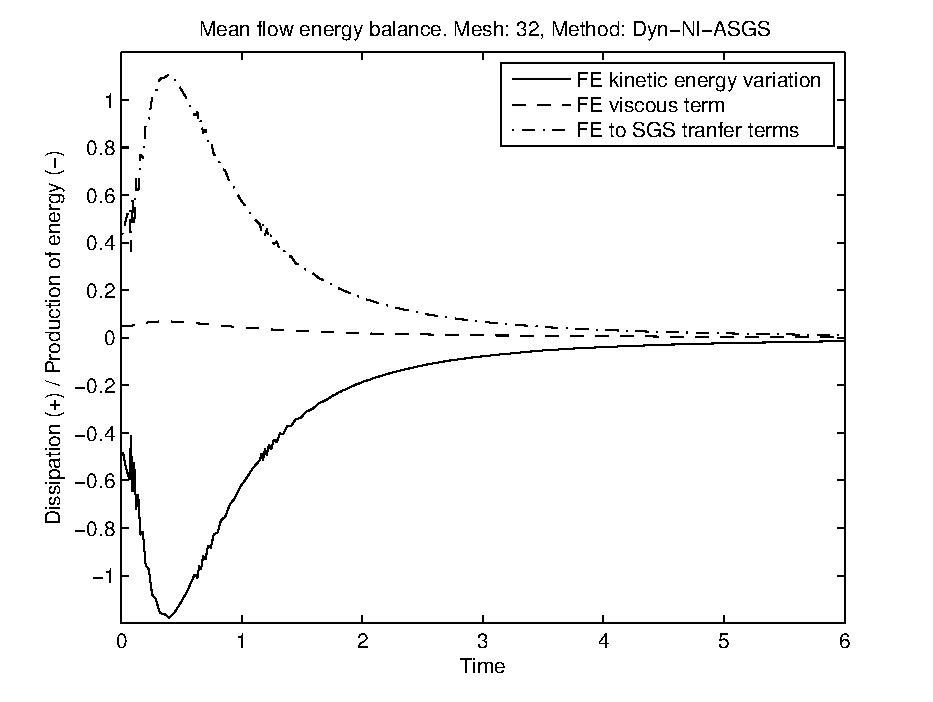
\includegraphics[width=0.49\textwidth]{Figures/DHIT/MF_ene_balance_ASGS_dyn_nl}}    
%  \subfigure[Subscale equation energy balance]{\label{fig:ASGS_ss_balance}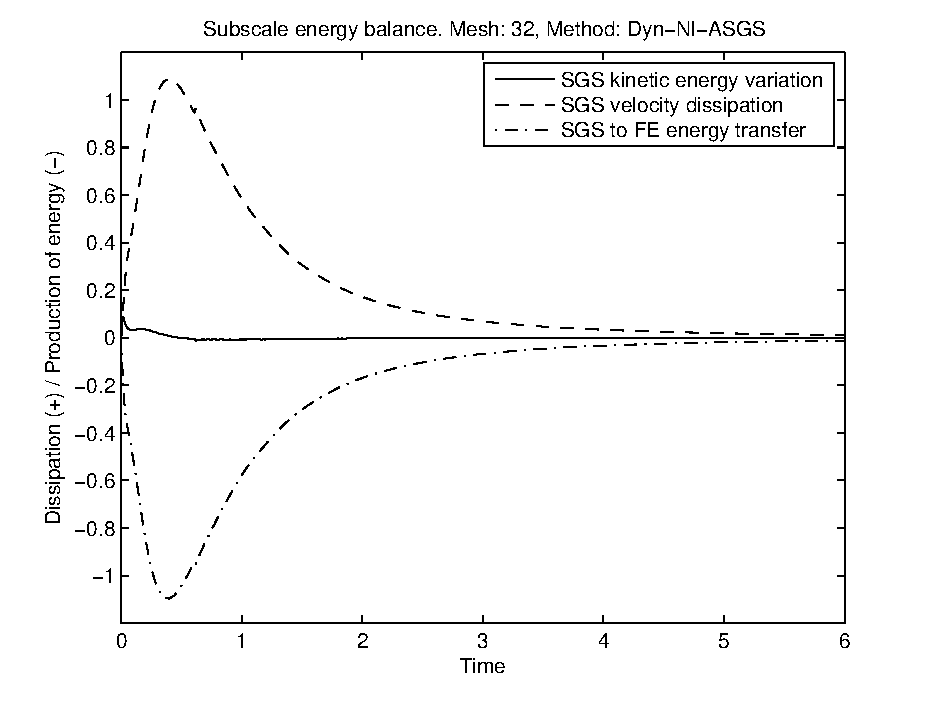
\includegraphics[width=0.49\textwidth]{Figures/DHIT/SS_ene_balance_ASGS_dyn_nl}}
%  \caption{Mean flow and subscale energy balances for the Dyn-Nl-ASGS method.}
%  \label{fig:ASGS_ene_balance_split}
%\end{figure}

%Note that some oscillations in the FE time derivative term and FE to SS transfer terms
%can be observed in Fig. \ref{fig:ASGS_MF_balance}.{\color{blue}They can be explained by the coupling between temporal derivatives for the ASGS method in equation (\ref{eq-C4_time_deriv_ASGS}). No lo veo claro.}

%In order to check 
The energy balance evolution for the mean flow and the subscales equations in (\ref{eq-C4_FE_balance2})-(\ref{eq-C4_sgs_balance2}) for the Dyn-Nl-OSS case are shown in Fig. \ref{fig:OSS_ene_balance_split}. Fig. \ref{fig:OSS_MF_balance} depicts the energy balance evolution for the mean flow equation. Like for the ASGS method, the loss of kinetic energy is balanced by the FE scales to subscales energy transfer terms. The FE viscous term also has a very little impact on the dissipation of energy. On the other side, the subscales energy balance shown in Fig. \ref{fig:OSS_ss_balance} shows that almost all the energy transferred by the FE to the subscales is offset by the subscale velocity term,
again like in the ASGS method.
%by the subscale viscous term, also 
%like the ASGS method. Is important to say that the FE to SGS and SGS to FE energy transfer terms do not have any time derivative contribution, which do happen for the ASGS method. {\color{blue}This fact has a direct implication on the results since here, in the OSS method, there is no coupling between time derivative terms and we do not have oscillations.}
The only important difference between both methods is that \emph{no oscillations are observed in the FE kinetic energy evolution when the OSS method is used.}

%\begin{figure}[h!]
%  \centering
%  \subfigure[Mean flow equation energy balance]{\label{fig:OSS_MF_balance}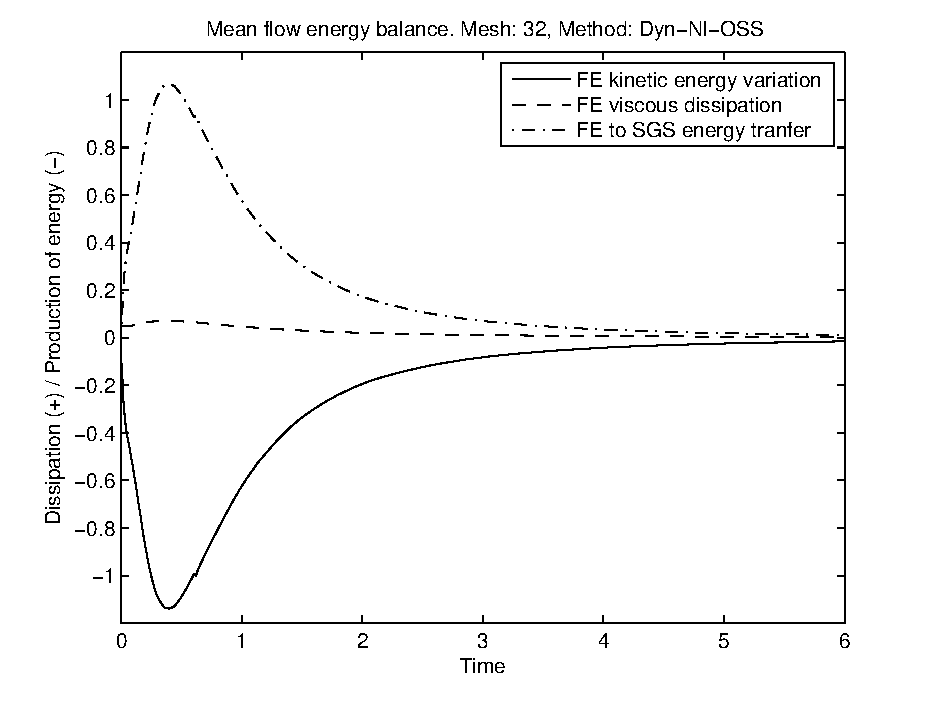
\includegraphics[width=0.49\textwidth]{Figures/DHIT/MF_ene_balance_OSS_dyn_nl}}    
%  \subfigure[Subscale equation energy balance]{\label{fig:OSS_ss_balance}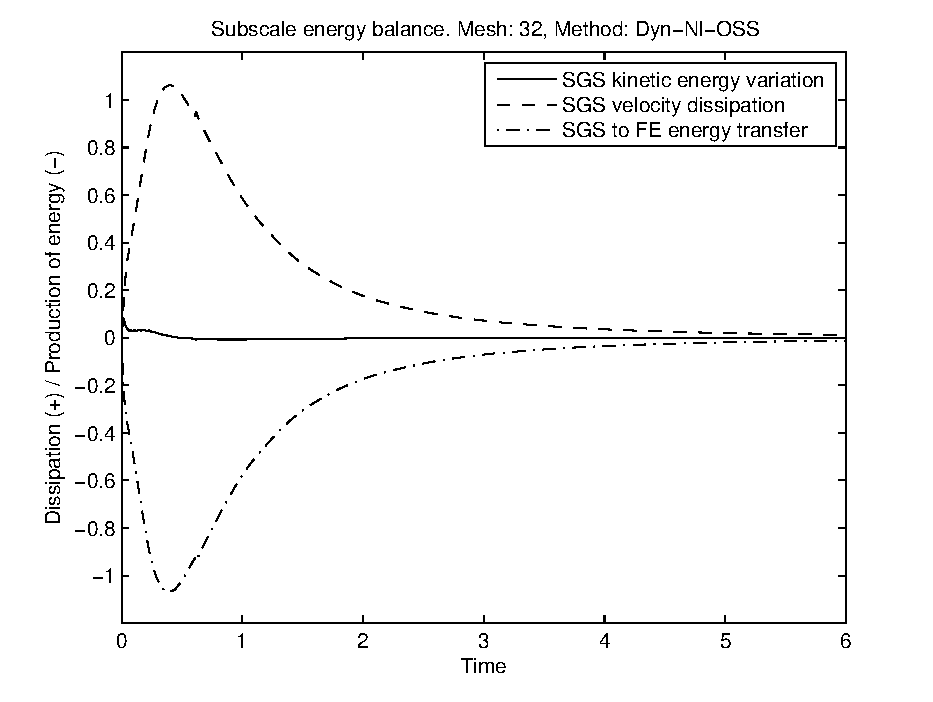
\includegraphics[width=0.49\textwidth]{Figures/DHIT/SS_ene_balance_OSS_dyn_nl}}
%  \caption{Mean flow and subscale energy balances the Dyn-Nl-OSS method.}
%  \label{fig:OSS_ene_balance_split}
%\end{figure}

The global energy balance terms obtained solving the problem with the skew-symmetric convective term \textit{type 2} for the Dyn-Nl-ASGS and Dyn-Nl-OSS cases are shown in Fig. \ref{fig:ene_balance_sk2}. We note that the loss of skew-symmetry in the convective term has a non-negligible effect (see Figs.~\ref{fig:ASGS_ene_balance2} and \ref{fig:OSS_ene_balance2}). In particular, this term introduces negative dissipation (production of energy) into the problem. %As we will show in Section \ref{subsubsec-C4_Total_ene_DHIT}, 
This fact implies that the method is less dissipative and the energy decays at a slower rate than using the convective term \textit{type 1} and the method seems to be less diffusive. This negative contribution, however, is not predictable and could result in a blow up of the calculation. We refer to Section \ref{sec-C4_effect_const} for further comments about numerical instabilities associated to the \textit{type 2} convective term.%Although no theoretical energy estimates are available we have not observed instabilities in practice.

%\begin{figure}[h!]
%	\centering	
%	\subfigure[Global energy balance for Dyn-Nl-ASGS]{\label{fig:ASGS_ene_balance2}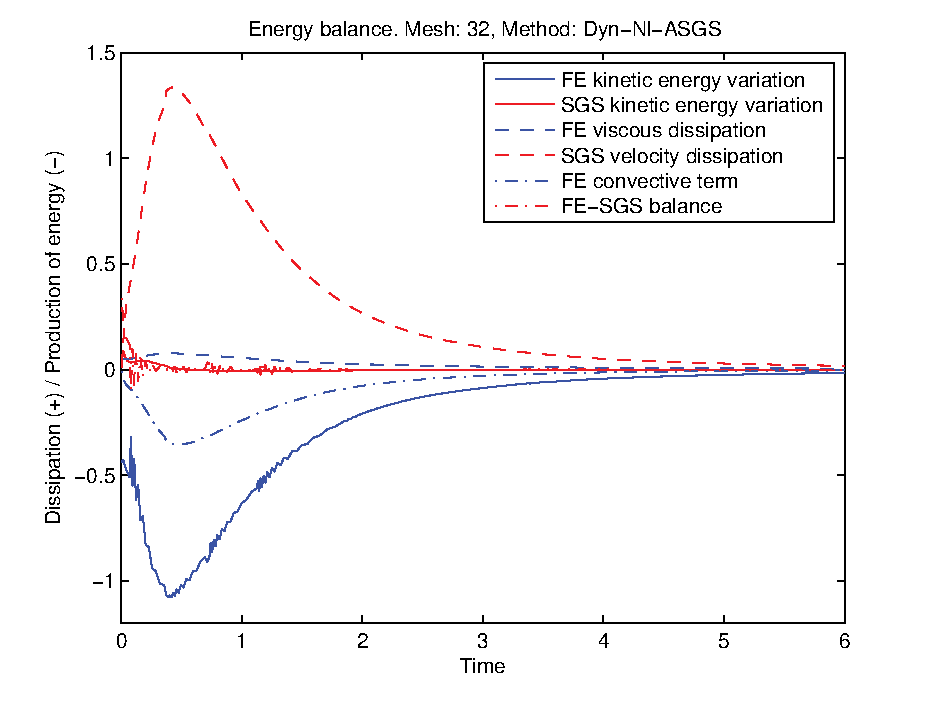
\includegraphics[width=0.49\textwidth]{Figures/DHIT/ene_balance_ASGS_sk2}}
%	\subfigure[Global energy balance for Dyn-Nl-OSS]{\label{fig:OSS_ene_balance2}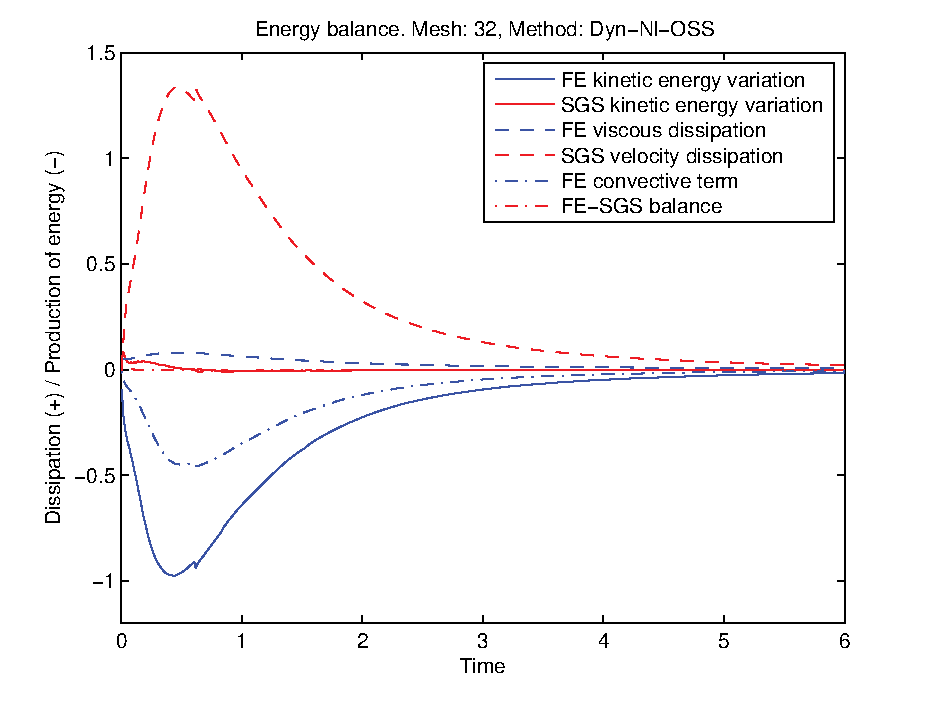
\includegraphics[width=0.49\textwidth]{Figures/DHIT/ene_balance_OSS_sk2}}
%	\caption{Global energy balance using skew-symmetric convective term \textit{type 2}.}
%	\label{fig:ene_balance_sk2}
%\end{figure}

\subsubsection{Computational cost analysis}

\label{subsubsec-C4_comp_cost_DHIT}
The actual implementation in the parallel FE multiphysics code FEMPAR \cite{Badia2013a} is based on a classical domain decomposition strategy. At each nonlinear iteration the monolithic linear system is solved using a classical GMRES method applied to the Schur complement over the interfaces of the subdomains. This iterative procedure is preconditioned using a balancing Neumann-Neumann method applied to the monolithic system. The cost of each iteration is that of local Dirichlet solves for the Schur complement application and a local Neumann solve and a global solve for the preconditioner application (see \cite{mandel_balancing_1993,dohrmann_preconditioner_2003,Badia2013}). All local systems are solved using the sparse direct solvers in PARDISO library \cite{Schenk2004,Schenk2006}.

An important issue when comparing different computational methods is their corresponding computational cost. In order to characterize the performance of the different VMS methods introduced in Section \ref{sec-C4_formulation},  we analyze  some quantities that define the computational cost of each method, viz. nonlinear iterations, iterative solver iterations, and the adaptive time step evolution.

%All cases compared here have been solved using a $32^3$ linear hexahedral element mesh. This discretization is very coarse and it allows us to stress the differences between the proposed methods. In fact, due to this discretization, the linear and static ASGS case (Sta-Lin-ASGS) and the dynamic and linear ASGS case (Dyn-Lin-ASGS) do not converge at $t=0.0$ and  $t=0.123$, respectively; the nonlinear iterations diverge even reducing the time step size. Anyway, all the methods converge as $h\rightarrow0$.

The cases compared here have been solved using $32^3$ and $64^3$ linear hexahedral element meshes. The $32^3$ discretization is very coarse but it allows us to stress the differences between the proposed methods. In fact, due to this discretization, the linear and static ASGS case (Sta-Lin-ASGS) and the dynamic and linear ASGS case (Dyn-Lin-ASGS) do not converge at $t=0.0$ and  $t=0.123$, respectively; the nonlinear iterations diverge even reducing the time step size. Anyway, all the methods converge as $h\rightarrow0$.

%The Nonlinear iterations needed at each time-step is a good measure of the computational cost. It can be seen that the ASGS method requires less nonlinear iterations at each time step compared with OSS, in which the number of iterations are greater for all the cases. Referring to the OSS method, we see that the dynamic cases, both linear and nonlinear, needs less iterations to achieve convergence without any significant difference between each other.

The number of nonlinear iterations needed at each time step by the ASGS method is smaller than the one required by the OSS method in all cases. This is due to the evaluation of the projections at the previous nonlinear iteration $i-1$; the implicit treatment of the projection is carried out by the nonlinear loop. Alternatively, since the projection is a linear operation, it can be performed together with the linear system \cite{Codina_2008a}, although a more involved implementation is required. Referring to the OSS method, we observe that the dynamic cases, both linear and nonlinear, need less iterations to achieve convergence without any significant difference between each other.

However, the number of nonlinear iterations is not the most relevant measure of the computational cost as the cost of each iteration is not fixed when iterative linear solvers are considered. Fig. \ref{fig:com_cost_DHIT} shows the accumulated number of solver iterations for each time step for the methods that have attained convergence with the $32^3$ mesh (Fig. \ref{fig:soliter32}) and for the dynamic versions with the $64^3$ mesh (Fig. \ref{fig:soliter64}). 
%The amount of nonlinear iterations required at each time step is a good computational cost measure, but we do not know if the iterations between methods are equivalent. In order to have an idea of the global computational cost, we must have also into account the solver iterations. In Fig. \ref{fig:Soliter} we display the maximum number of solver iterations for each time step for the converged cases. 
%Unlike the nonlinear iterations, here we see that the ASGS method requires more solver iterations than OSS. The maximum solver iterations at each time step for the dynamic and nonlinear ASGS case is highly variable, with values from around 50 to around 270. Meanwhile, all cases of the OSS method seem to remain almost constant around 70.  
%{\color{blue}
Unlike the nonlinear iterations, here we see that the ASGS method requires more solver iterations than OSS. The maximum solver iterations at each time step for the dynamic and nonlinear ASGS case is variable, starting from near 600, dropping to 200 and rising to around 300 iterations at the end of the computation. Meanwhile, all cases of the OSS method remain almost constant, around 60 iterations in the dynamic cases and around 40 iterations in the static one. The relation between time step size and solver iterations for each method is analyzed in Section \ref{sec-C4_small_time_step}. %}

%\begin{figure}[h!]
%	\centering	
%	%\subfigure[Maximum solver iterations at each time step]{\label{fig:Soliter}\includegraphics[width=0.49\textwidth]{Figures/DHIT/Soliter_32_scaled_cnvgd}}
%	%\subfigure[Accumulated solver iterations at each time step for]{\label{fig:Acsoliter}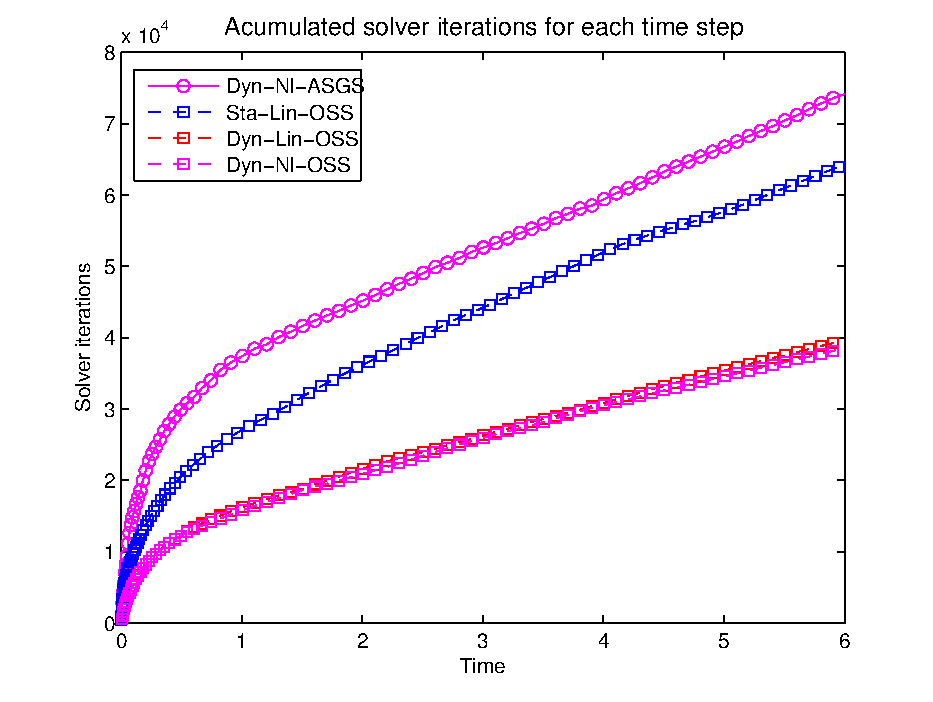
\includegraphics[width=0.49\textwidth]{Figures/DHIT/Acsoliter_32_scaled_cnvgd}}
%	%\caption{Maximum and accumulated solver iterations}
%	\subfigure[$32^3$ mesh]{\label{fig:soliter32}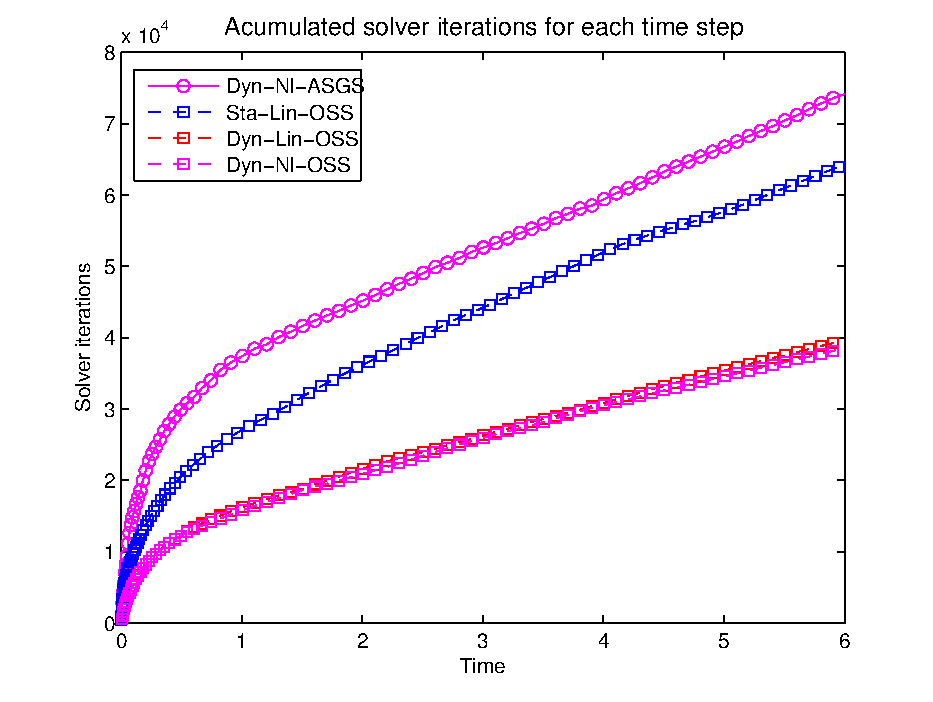
\includegraphics[width=0.49\textwidth]{Figures/DHIT/Acsoliter_32_scaled_cnvgd}}
%	\subfigure[$64^3$ mesh]{\label{fig:soliter64}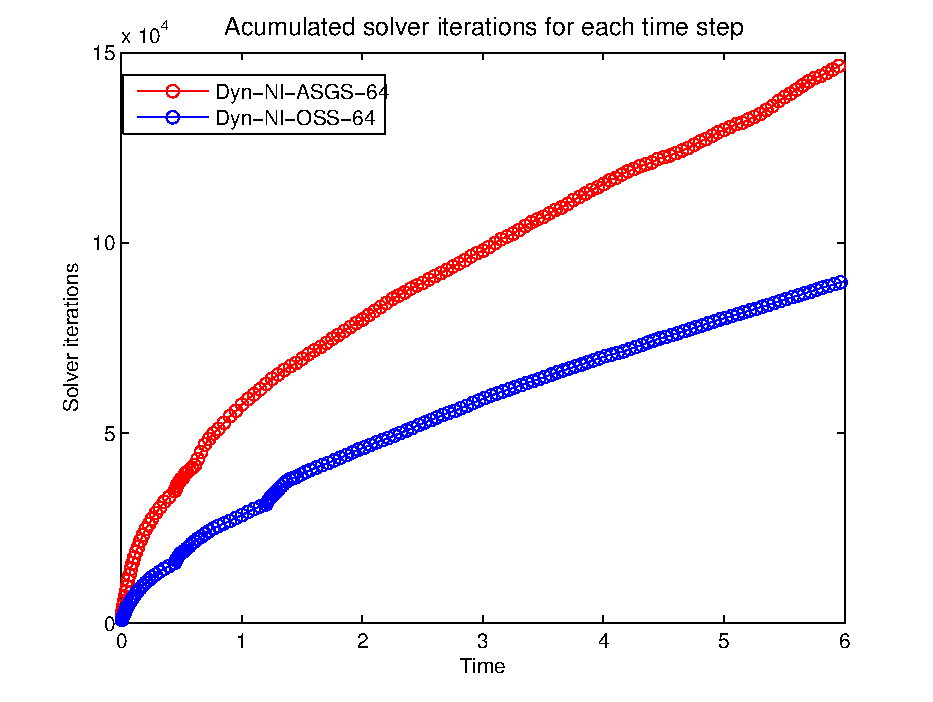
\includegraphics[width=0.49\textwidth]{Figures/DHIT/Acsoliter_64}}
%	\caption{Accumulated solver iterations.}
%	\label{fig:com_cost_DHIT}
%\end{figure}

%The adaptive time stepping described in the previous subsection has an important role on the computational cost, as mentioned earlier. If the time step is reduced in order to ensure convergence, the global computational cost is increased. Then, we are looking for those methods that do not require time step reductions, consequently reducing the total amount of time step evaluations. There are some methods that need to reduce the time step to keep  convergence, which can be noticed  in Fig. \ref{fig:Soliter} by a sudden reduction of the solver iterations or in Fig. \ref{fig:Acsoliter} by the density of the points. It is seen in Fig. \ref{fig:com_cost_DHIT} that ASGS schemes perform worse than OSS counterparts in this respect. Comparing the dynamic and nonlinear cases for both methods, we see that ASGS needs to reduce more than twice the time step, while  OSS only twice. As it has been said before, the linear cases for ASGS, both static or dynamic, have not converged at certain time steps. In what refers to the linear cases for the OSS method, there is not any reduction of the time step, rather it is constantly increasing until the threshold.
%{\color{blue}
The adaptive time stepping described in the previous subsection has an important role on the computational cost, as mentioned earlier. If the time step is reduced in order to ensure convergence, the global computational cost is increased. Then, we are looking for those methods that do not require time step reductions, consequently reducing the total amount of time step evaluations. In this case, any of the methods shown in Fig. \ref{fig:soliter32} need to reduce the time step. Since we do not have any time step reduction and the number of solver iterations per step is stabilized after $t=1$ for the $32^3$ mesh and $t=1.5$ for the $64^3$ mesh, the total amount of accumulated solver iterations (in nonlinear and time loops) shown in Fig. \ref{fig:com_cost_DHIT} increases almost linearly. We see in this figure that the ASGS scheme performs worse than OSS in this aspect, with a steeper slope in both the  $32^3$ and the $64^3$ meshes. With respect to the OSS method, we see that the number of nonlinear iterations needed by the static version of this method results in a steeper slope of the accumulated solver iterations. No significant differences appear between the dynamic linear and nonlinear definitions of the OSS method.

Summarizing, ASGS methods need less nonlinear iterations (due to the treatment of the projections in the OSS method), but on the other hand  OSS methods need less solver iterations. Furthermore, \emph{ASGS formulations are prone to instabilities; linear formulations diverge and the nonlinear dynamic formulation requires much more solver iterations.}

We can clearly state that the most efficient method for this setting, in terms of computational cost, is the dynamic (both linear and nonlinear) OSS method; all OSS cases are below ASGS. It has to be said that the dynamic nonlinear OSS case requires less nonlinear iterations in some of the time step computations.
%}

\subsubsection{Total energy evolution}
\label{subsubsec-C4_Total_ene_DHIT}
In this section we present the total energy evolution of the resolved scales, i.e., the FE component. The results are shown in Fig. \ref{fig:total_ene} for the $32^3$ and the $64^3$ grids. We observe that all methods have a very similar accuracy for this test case, still far from the DNS result. The difference between the methods becomes even smaller when the mesh is refined and they are all closer to the DNS solution. Note that we do not plot the non-converged results from the ASGS static cases.

% SB: PUT A COMMENT?
%{\color{blue} Hay que pensar en el comentario que me hicieron en la ultima charla: no hay que comparar contra DNS sino contra DNS filtrado. Ver Sagaut secciones 9.1.1 and 9.2.1. }

%\begin{figure}[h!]
%	\centering	
%	% \subfigure[Using the skew-symmetric term \textit{type 1}]{\label{fig:total_ene_32_sk1}\includegraphics[width=0.49\textwidth]{Figures/DHIT/total_ene_32_scaled}}
%	% \subfigure[Using the skew-symmetric term \textit{type 2}]{\label{fig:total_ene_32_sk2}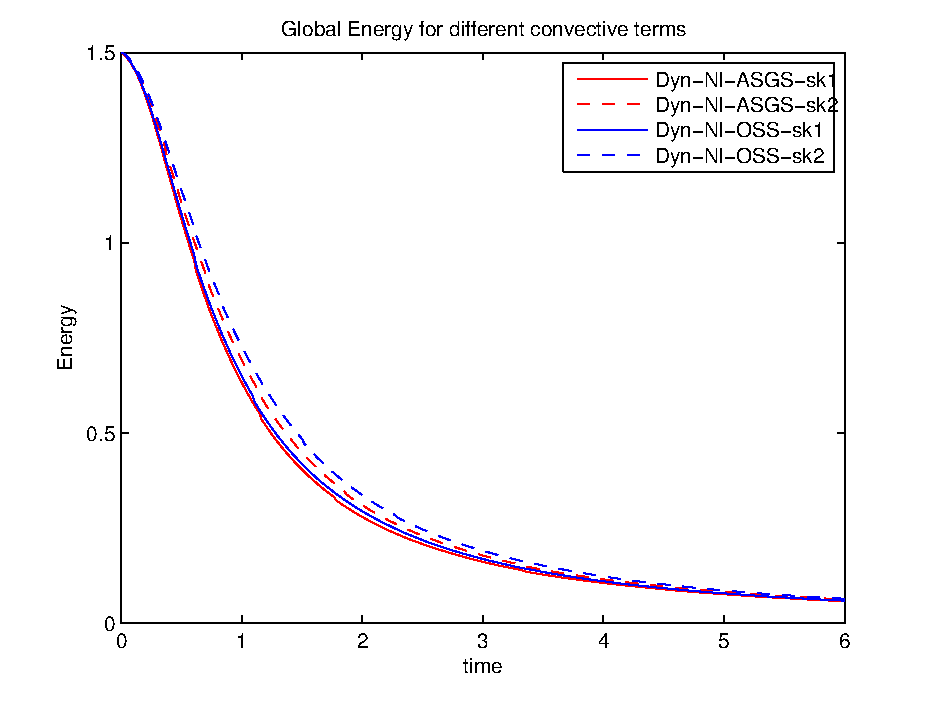
\includegraphics[width=0.49\textwidth]{Figures/DHIT/ene_skew_scaled}}
%	% \caption{Total energy evolution for a $32^3$ elements mesh with the scaled initial condition}
%	% \label{fig:total_ene_32}
%	\subfigure[$32^3$ mesh]{\label{fig:total_ene_32}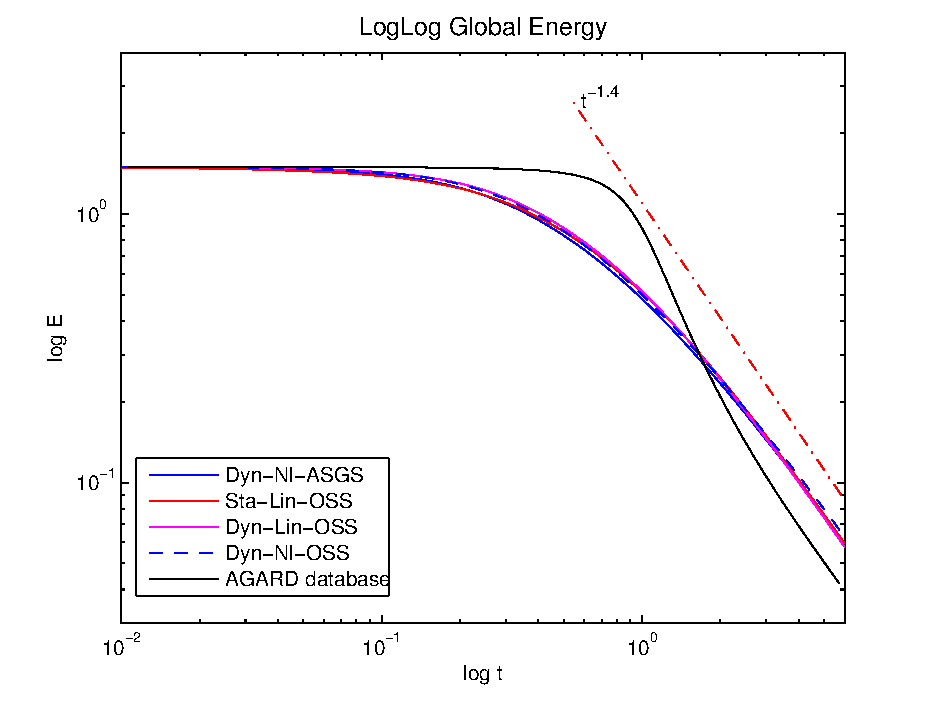
\includegraphics[width=0.49\textwidth]{Figures/DHIT/total_ene_32_scaled_loglog.pdf}}
%	\subfigure[$64^3$ mesh]{\label{fig:total_ene_64}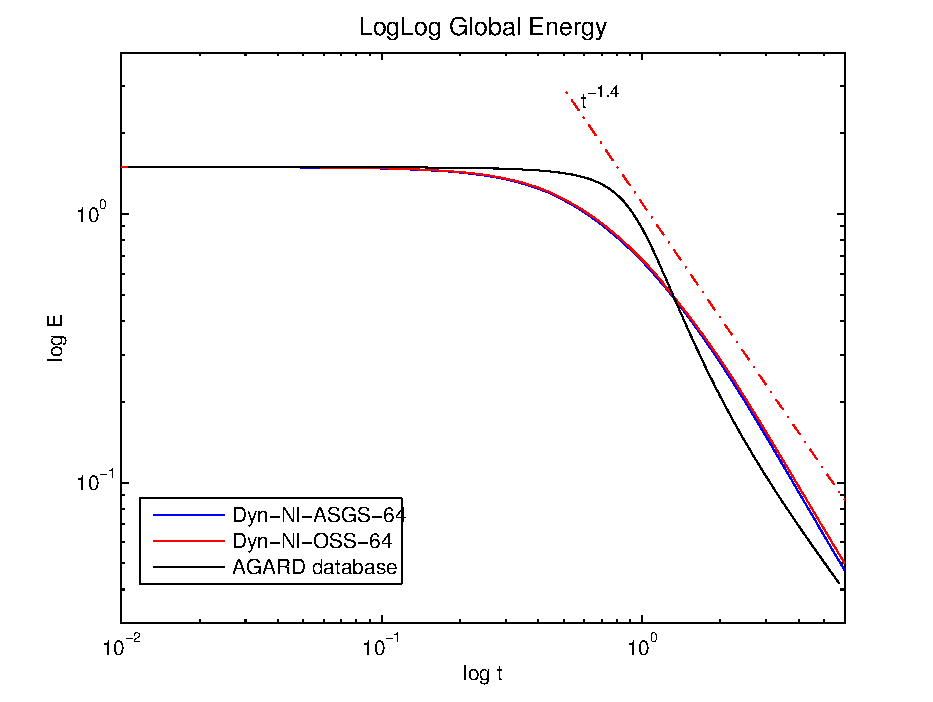
\includegraphics[width=0.49\textwidth]{Figures/DHIT/total_ene_64_scaled_loglog.pdf}}
%	\caption{Total energy evolution for the $32^3$ and $64^3$ elements meshes with the scaled initial condition.}
%	\label{fig:total_ene}
%\end{figure}

%The results shown so far have been obtained using the skew-symmetric convective term \textit{type 1} defined in (\ref{eq-C4_b_skew1}). 
%But what happens if we choose another definition for this term? We know, by some experience acquired on other tests not reported in this work, e.g. Destabilization of an ordered initial condition test (2D and 3D), that the nonskew-symmetric term (\ref{eq-C4_b_noskew}) can involve convergence problems. So 
%We test the influence of this term by solving the same problem with the convective skew-symmetric term (\textit{type 2)}  in (\ref{eq-C4_b_skew2}) for dynamic and nonlinear ASGS and OSS schemes. The results obtained for this test are shown in Fig. \ref{fig:total_ene_32_sk2}, where it is seen that the solution using the \textit{type 2} term is above the one obtained with term \textit{type 1}, which shows that the convective term is actually productive.
%. Then, we can say that the solution is less dissipative when we use this convective term which agree with the results shown in the energy conservation analysis done in subsection \ref{subsubsec-C4_ene_cons_DHIT}. This result is a consequence of the fact that the convective term is non zero as it is exposed on remark \ref{rem:skewsym}, equation (\ref{eq-C4_mkgkdfsnmgks}).

\subsubsection{Energy spectra}
According to \cite{mansour_decay_1994}, the resolution of the small scales in isotropic decaying turbulence is judged by the shape of the energy spectra at high wave numbers, and requires 
%that the total amount of wave numbers should be such that 
$k_{max}\eta\approx1$, $\eta=(\nu^3/\epsilon)^{1/4}$ being the Kolmogorov length scale and $k_{max}$ the maximum wave number required. In this case $k_{max}\approx182$, which means at least a $300^3$ FE mesh for a DNS computation, with a high computational cost.
%, so here it is shown the importance of a good LES method, which allow us to have good results on the energy containing eddies and the inertial subrange without solving the small scales.
%If we want to see if our VMS method is able to behave like a LES, we should be able to show that on the inertial subrange, the energy spectra follows the Kolmogorov law
%$$E(k)\propto\epsilon^{2/3}k^{-5/3}.$$
In this section we evaluate the capability of the VMS method to represent the energy of the  eddies at the inertial subrange without solving the small scales and compare the results against Kolmogorov's law prediction
$$E(k)\propto\epsilon^{2/3}k^{-5/3},$$
$E$ being the turbulent kinetic energy.

In Fig. \ref{fig:spec_32_64} the energy spectra for the different cases described in Table \ref{table:DHIT_cases}, using $32^3$ and $64^3$ linear hexahedral element mesh are presented. 
%Leaving aside the total energy evolution, which for this discretization is far to be considered acceptable, 
% {\color{blue}
We can see in Fig. \ref{fig:spec_32} that the energy spectra at $t=0.2$ decays with a different slope depending on the VMS method used. Although the differences are small and only appear at large wavenumbers, we see that the dynamic OSS models are less dissipative than the Dyn-Nl-ASGS and Sta-Lin-OSS ones. 
For the finer $64^3$ mesh the difference between the spectra obtained using Dyn-Nl-ASGS and Dyn-Lin-OSS are even smaller, as shown in Fig. \ref{fig:spec_64}; OSS is again less dissipative.
%The Dyn-Lin-OSS method seems to follow the $k^{-5/3}$ Kolmogorov law better at this time, but the Dyn-Nl-OSS case also have a good agreement with the Kolmogorov law for intermediate scales. %}

%\begin{figure}[h!]
%  \centering
%  \subfigure[$32^3$ mesh]{\label{fig:spec_32}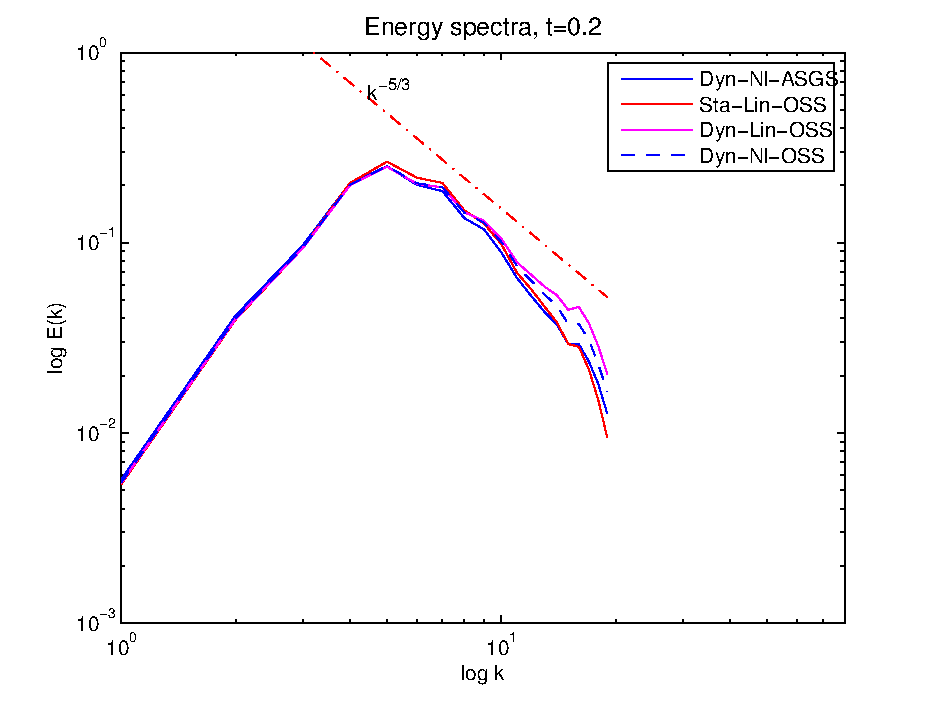
\includegraphics[width=0.49\textwidth]{Figures/DHIT/spec_32_02_scaled}}    
%  \subfigure[$64^3$ mesh]{\label{fig:spec_64}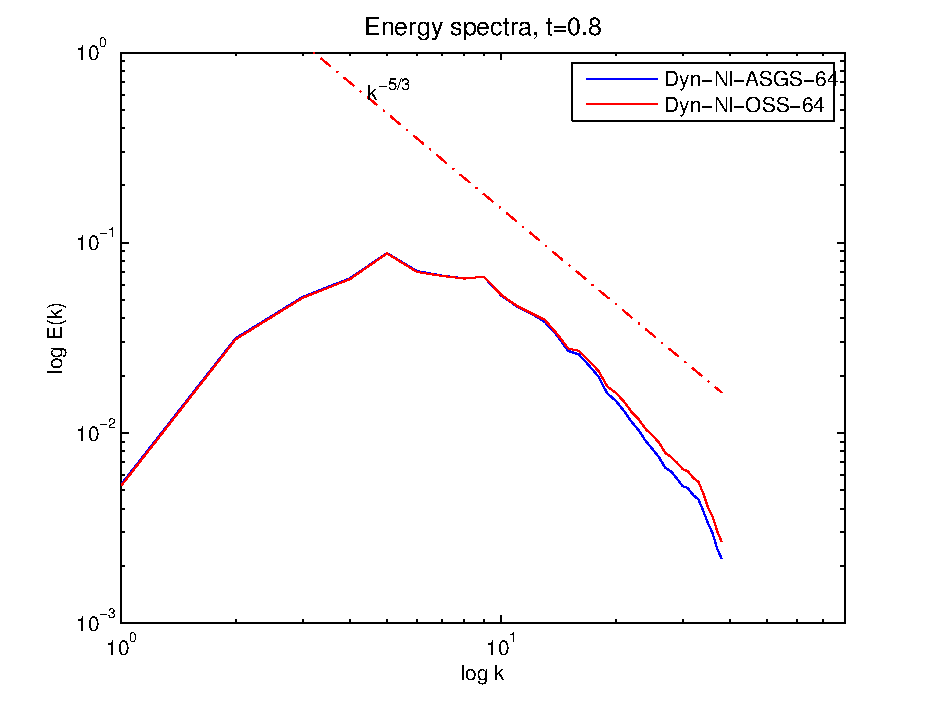
\includegraphics[width=0.49\textwidth]{Figures/DHIT/spec_64_08}}
%%  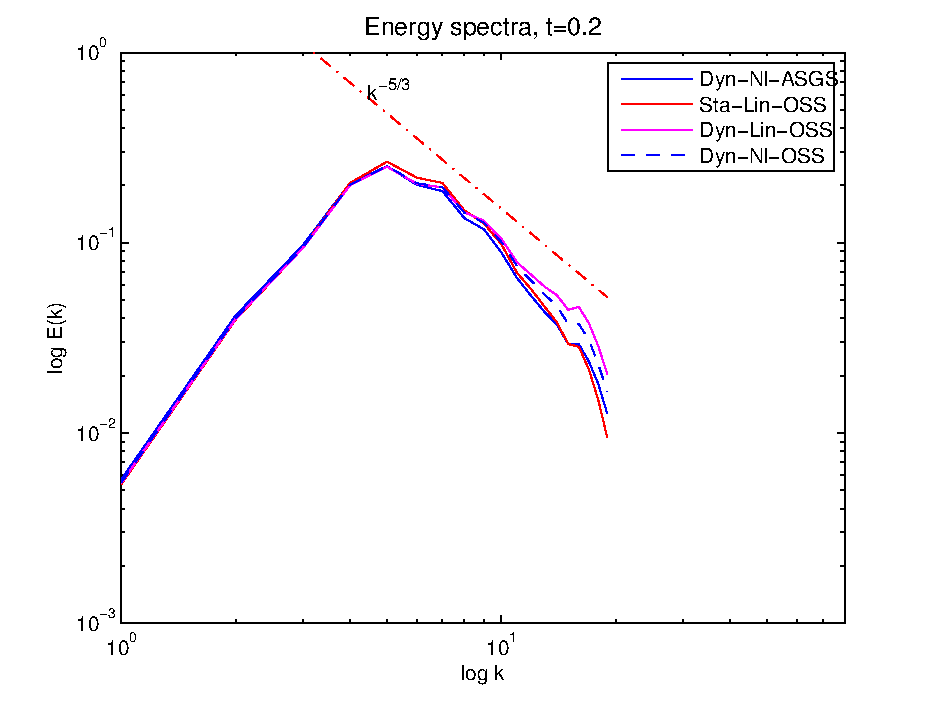
\includegraphics[width=0.5\textwidth]{Figures/DHIT/spec_32_02_scaled}
%  \caption{Energy spectra at $t=0.2$ ($32^3$ mesh) and $t=0.8$ ($64^3$ mesh).}
%  \label{fig:spec_32_64}
%\end{figure}

\subsubsection{$h$-$p$ refinement}

The energy decay computed using $32^3$ and $64^3$ linear FE meshes is far from the one obtained using DNS \cite{_selection_????}, as shown in Fig. (\ref{fig:total_ene}) and discussed above. To make clear that these poor results are due to this crude discretization,
%We have seen in Fig. \ref{fig:total_ene_32_sk1} that the total energy computed using a $32^3$ elements mesh is far from the one showed in the DNS \cite{_selection_????}. We also have said before that the initial total energy for this problem is highly mesh dependent. Thus, we expect that when we refine the mesh we will get a better initial energy approximation which will improve the whole energy evolution. Then, the results should become closer to the DNS.
%To check this assumption we perform 
we present a mesh refinement analysis, both reducing the element length $h$ and increasing the interpolation order $p$.
% (here $p$ is not the pressure field). 
We choose the Dynamic and Nonlinear OSS method (Dyn-Nl-OSS), which is the one that shows the lowest slope in the accumulated iterations evolution (Fig. \ref{fig:com_cost_DHIT}) for the $32^3$ and $64^3$ linear elements mesh. We solve the problem using the discretizations exposed in Table \ref{table:refinement}.

\begin{table}[h]
\centering
\begin{tabular}{ccc}
\hline
Label&Mesh elements&Element type\\
\hline
32 ($Q$1)&$32^3$&hexahedral linear ($Q1$)\\
64 ($Q$1)&$64^3$&hexahedral linear ($Q1$)\\
128 ($Q$1)&$128^3$&hexahedral linear ($Q1$)\\
32 ($Q$2)&$32^3$&hexahedral quadratic ($Q2$)\\
64 ($Q$2)&$64^3$&hexahedral quadratic ($Q2$)\\
32 ($Q$3)&$32^3$&hexahedral cubic ($Q3$)\\
\hline
\end{tabular}
\caption{$h$-$p$ refinement cases.}
\label{table:refinement}
\end{table}

%To check this assumption we can refine the mesh in two different ways. On one hand, we can decrease $h$, that is to increase the number of mesh elements for each direction. On the other hand, we can use higher order elements, e.g. $Q2$ or $Q3$. We do this analysis using the Dynamic and Nonlinear OSS method (Dyn-Nl-OSS), which is the one that shows the best results for the $32^3$ linear elements mesh. We solve the problem using the following discretizations:
%\begin{itemize}
%\item[-] $32^3$ hexahedral trilinear elements ($Q1$).
%\item[-] $64^3$ hexahedral trilinear elements ($Q1$).
%\item[-] $128^3$ hexahedral trilinear elements ($Q1$).
%\item[-] $32^3$ hexahedral triquadratic elements ($Q2$).
%\item[-] $64^3$ hexahedral triquadratic elements ($Q2$).
%\item[-] $32^3$ hexahedral tricubic elements ($Q3$).
%\end{itemize}

In Fig. (\ref{fig:ene_hp}) we show the total kinetic energy evolution obtained using the discretizations defined in Table \ref{table:refinement}. Reducing the mesh size $h$ and/or increasing the polynomial order $p$ (not to be confused with the pressure) the result becomes closer to the DNS, as expected. In Fig. \ref{fig:ene_hp_close} three groups can be clearly observed, namely 32 ($Q$1), 32 ($Q$2) and 64 ($Q$1) and the remaining three. The best results are obtained using $Q$2 elements although the difference is really small.
%The refinement on $h$ and $p$ not only has effect on the initial energy, but also on the time evolution. When we reduce $h$ or increase $p$ the total kinetic energy evolution becomes closer to the DNS one. It also must be said that the refinement on $p$ is more effective than the refinement on $h$, which is a consequence of the enrichment of the FE space that is achieved when we increase $p$. 

%\begin{figure}[h!]
%  \centering
%  % \subfigure[Total evolution]{\label{fig:ene_hp_global}\includegraphics[width=0.49\textwidth]{Figures/DHIT/ene_hp_scaled}}    
%  % \subfigure[Close up view]{\label{fig:ene_hp_close}\includegraphics[width=0.49\textwidth]{Figures/DHIT/ene_hp_close_scaled}}
%  % \caption{Total kinetic energy evolution}
%  \subfigure[Total evolution]{\label{fig:ene_hp_global}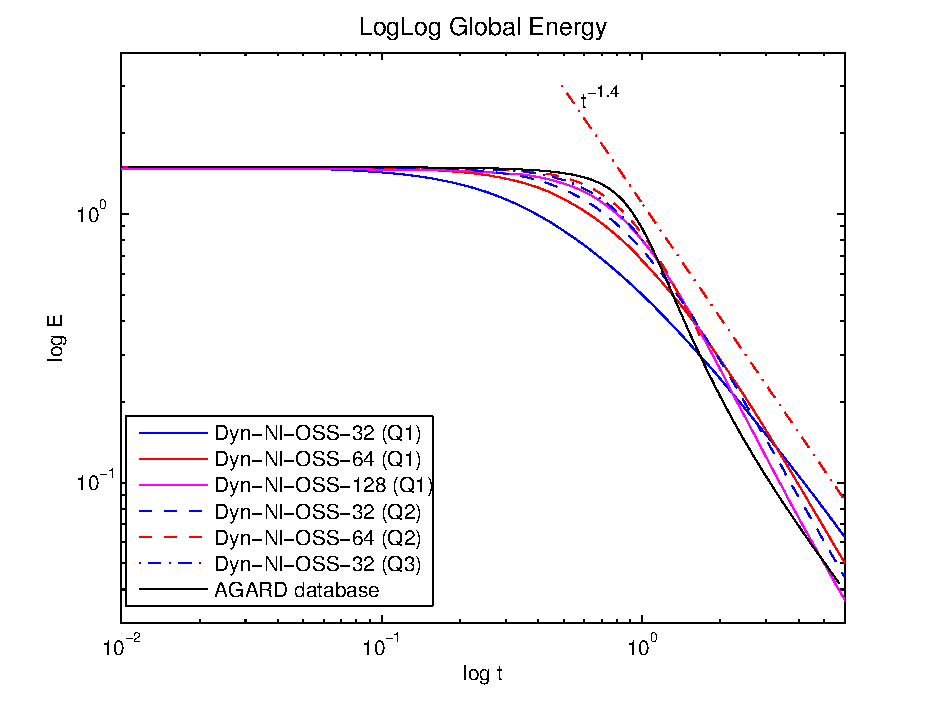
\includegraphics[width=0.49\textwidth]{Figures/DHIT/ene_hp_scaled_loglog}}    
%  \subfigure[Close up view]{\label{fig:ene_hp_close}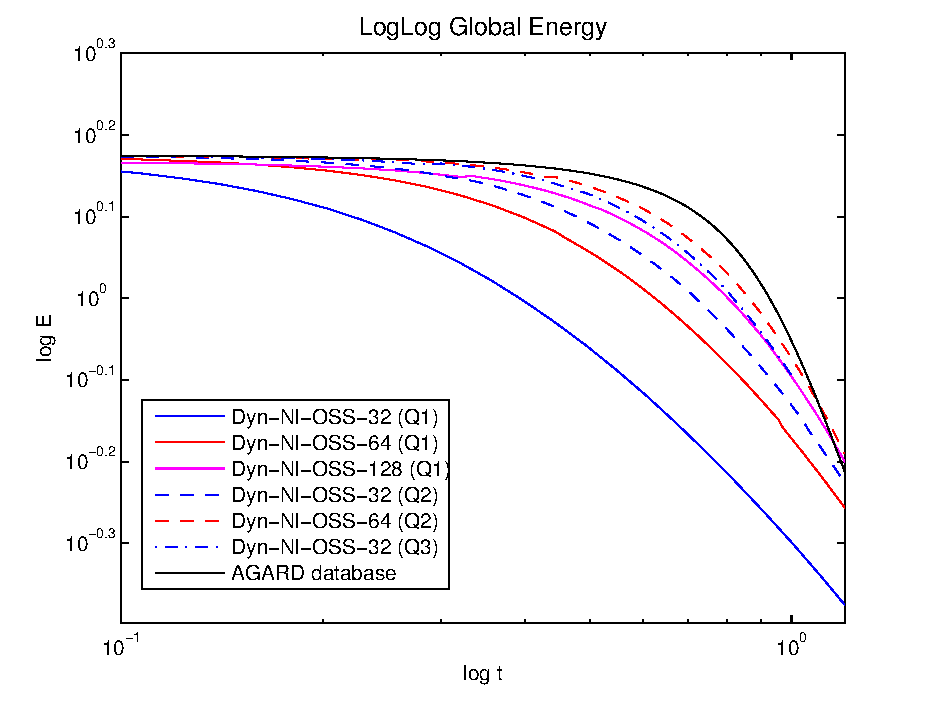
\includegraphics[width=0.49\textwidth]{Figures/DHIT/ene_hp_close_scaled_loglog}}
%  \caption{Total kinetic energy evolution.}
%  \label{fig:ene_hp}
%\end{figure}

%With respect to the energy spectra, we expect to be related with the different kinetic energy evolutions showed in Fig. \ref{fig:ene_hp}. It means that if the total kinetic energy decays earlier, the energy spectrum must evolve to the $k^{-5/3}$ law earlier. If we think it on the opposite sense, that would suppose that the small scales are dissipating energy on a earlier stage, which implies a premature decaying of the total kinetic energy. In Fig. \ref{fig:spec_hp} we show the energy spectra at time $t=0.2$, $t=0.4$ and $t=0.8$ for the different cases presented before.

Given the differences in the total energy evolution the time at which the $k^{-5/3}$ law is achieved differs for the different methods. We show the energy spectra at time $t=0.8$ and $t=1.0$ for the different cases presented before in Fig. \ref{fig:spec_hp}. As it can be observed in Fig.~\ref{fig:spec_hp_08}, at $t=0.8$, only the energy spectra obtained using the 32 ($Q1$) and  64 ($Q1$) have a steeper slope, while the other cases are almost parallel to the $k^{-3/5}$ line. This is what was expected since the kinetic energy decay occurs earlier in the coarser cases.
%Effectively, we can see that the results in Fig. \ref{fig:spec_hp} performs as predicted by the total energy evolution. At Fig. \ref{fig:spec_hp_02}, $t=0.2$, the energy cascade for the case Dyn-Nl-OSS-32 ($Q1$) is parallel to the $k^{-3/5}$ line, while the other cases still preserve the energy on the low wavenumbers. This behavior is consistent with the results shown in Fig. \ref{fig:ene_hp}, where the total kinetic energy for the case Dyn-Nl-OSS-32 ($Q1$) decays earlier than all the other methods.
%At $t=0.4$, as shown in Fig. \ref{fig:spec_hp_04}, the cases with $64^3$ nodes follow the $k^{-5/3}$ law but those cases with more nodes still have the energy on the large eddies and, on the other hand, the case with less nodes has dissipated a large part of it through small scales. Finally, Fig.\ref{fig:spec_hp_08} shows us that the energy spectra for those cases with a finer mesh has a proper energy cascade at $t=0.8$.
%{\color{blue}
%At $t=0.4$, as shown in Fig. \ref{fig:spec_hp_04}, the $32$ (Q1) case has the right energy decay slope, while for the cases with more degrees of freedom the contribution of the small scales to the energy is still increasing. Finally, Fig.~\ref{fig:spec_hp_08} shows us that the energy spectra for all cases has a proper energy cascade.
%At $t=0.8$ all the cases present a proper energy spectra, as shown in Fig.~\ref{fig:spec_hp_08}.
In Fig. \ref{fig:spec_hp_1} we show the energy spectra at $t=1.0$, and compare it against the DNS spectrum from \cite{_selection_????} at the same time step. It can be observed that the results tend to the DNS one as we increase resolution, being the $64(Q2)$ case the most accurate one.

Note that the DNS spectra is not present in Fig. \ref{fig:spec_hp_08} because it is not available in the database \cite{_selection_????} at this time step.

%\begin{figure}[h!]
%  \centering
%%  \subfigure[Energy spectra at $t=0.2$]{\label{fig:spec_hp_02}\includegraphics[width=0.49\textwidth]{Figures/DHIT/spec_hp_02}}    
%%  \subfigure[Energy spectra at $t=0.4$]{\label{fig:spec_hp_04}\includegraphics[width=0.49\textwidth]{Figures/DHIT/spec_hp_04}}
%  \subfigure[Energy spectra at $t=0.8$]{\label{fig:spec_hp_08}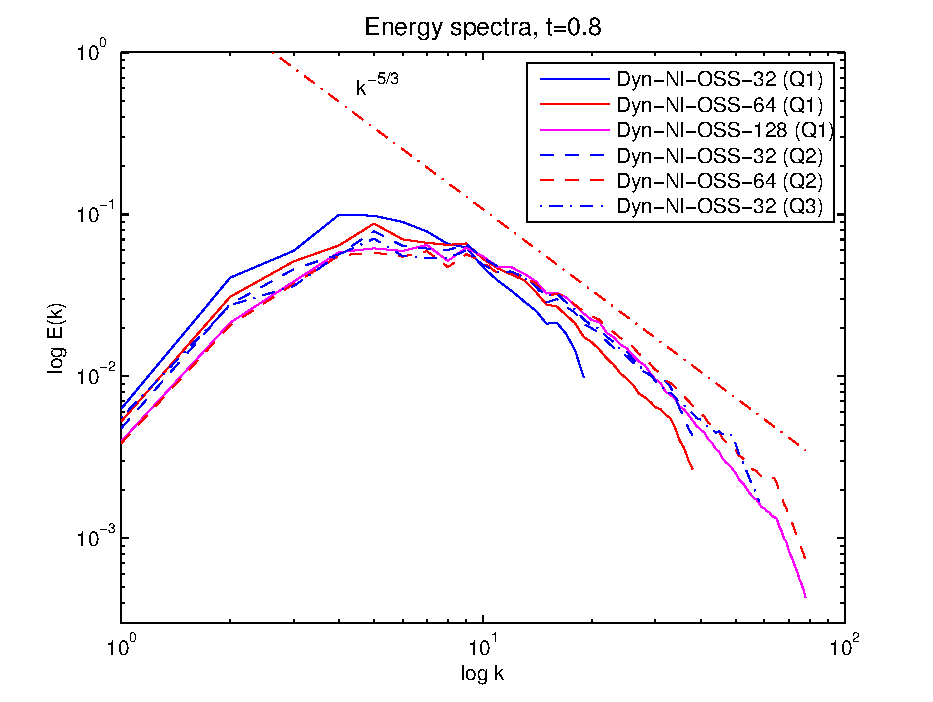
\includegraphics[width=0.49\textwidth]{Figures/DHIT/spec_hp_08}}
%  \subfigure[Energy spectra at $t=1.0$]{\label{fig:spec_hp_1}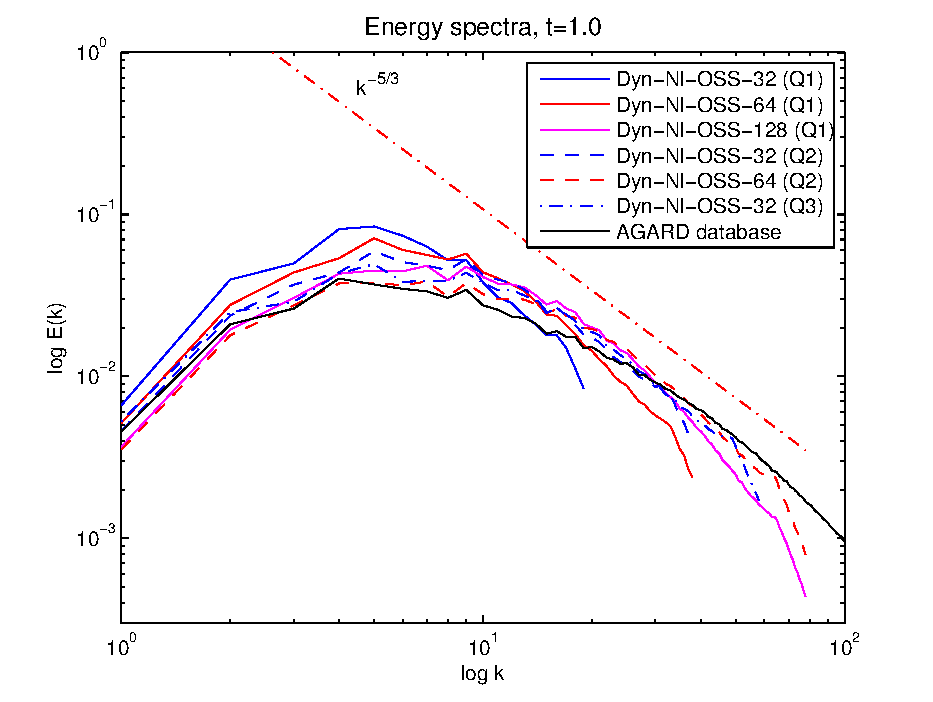
\includegraphics[width=0.5\textwidth]{Figures/DHIT/spec_hp_1}}
%  \caption{Energy spectra at $t=0.8$ and $t=1.0$ for the $h$-$p$ refinement defined in Table~\ref{table:refinement}.}
%  \label{fig:spec_hp}
%\end{figure}

 \subsubsection{Comparison with a non-stabilized method}

% All the results presented up to this point have been computed using a VMS method, either ASGS or OSS. But, what would be the result using other methods? Are the methods presented here, comparable with classical LES methods? Which methods perform better? To answer all these questions, we have solved the problem adding a physical model without stabilization. To do that, an inf-sup stable element is needed and we have used the Taylor-Hood $Q2/Q1$ element. 
 %This element also has the unknowns at the nodes but uses shape functions of degree $2$ for the velocity degrees of freedom and shape functions of degree $1$ for the pressure DOFs. This type of element give stable results when we solve non convection dominated flows only taking into account the Galerkin terms.
 %We are solving a turbulent problem, so we must add a LES model to the Galerkin formulation in order to take into account the effect of the small scales on the flow when we solve it in a coarse mesh. 
 We use the classical static Smagorinsky model, consisting in adding a turbulent viscosity $\nu_t$ that depends on the velocity gradient and the characteristic element length $h$. This additional viscosity also acts as stabilization of convection, as usual in standard LES simulations. Then, we have to solve the standard Galerkin problem using Taylor-Hood $Q2/Q1$ elements and introducing a modified viscosity defined as
 \begin{equation}
 \label{eq-C4_nu_smago}
 \nu = \nu_l+\nu_t,
 \end{equation}
 where $\nu_l$ is the real flow viscosity and $\nu_t=(C_sh)^2|\nabla^s\u|$. $C_s$ is the Smagorinsky constant, which we set equal to $0.15$.

% In Fig. \ref{fig:ene_spec_q2q1} we show the total kinetic energy time evolution and the energy spectra of this method compared with the dynamic and nonlinear OSS method. In particular, we show the results for those cases from Table \ref{table:refinement} such that they have $65^3$ velocity nodes.
 We can see in Fig. \ref{fig:ene_q2q1} that the total kinetic energy is decaying faster for the non-stabilized method than for the OSS method. This behavior is directly related to the shape of the energy spectra in Figs. \ref{fig:spec_q2q1_02}-\ref{fig:spec_q2q1_08}, where we can see that the Smagorinsky method presents lower values of energy at $t=0.4$. It is important to point out the pile-up that appears in the Smagorinsky spectra, denoting that small scales are not dissipating energy properly.

% \begin{figure}[h!]
%   \centering
%   \subfigure[Energy evolution]{\label{fig:ene_q2q1}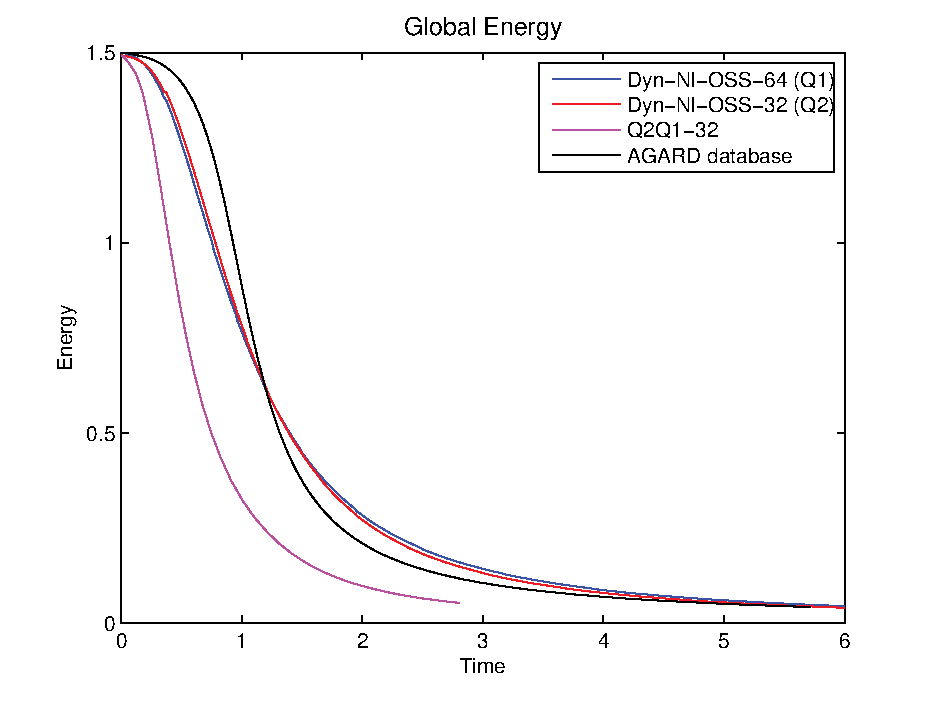
\includegraphics[width=0.49\textwidth]{Figures/DHIT/ene_q2q1_scaled}}  
%   \subfigure[Energy spectra at $t=0.2$]{\label{fig:spec_q2q1_02}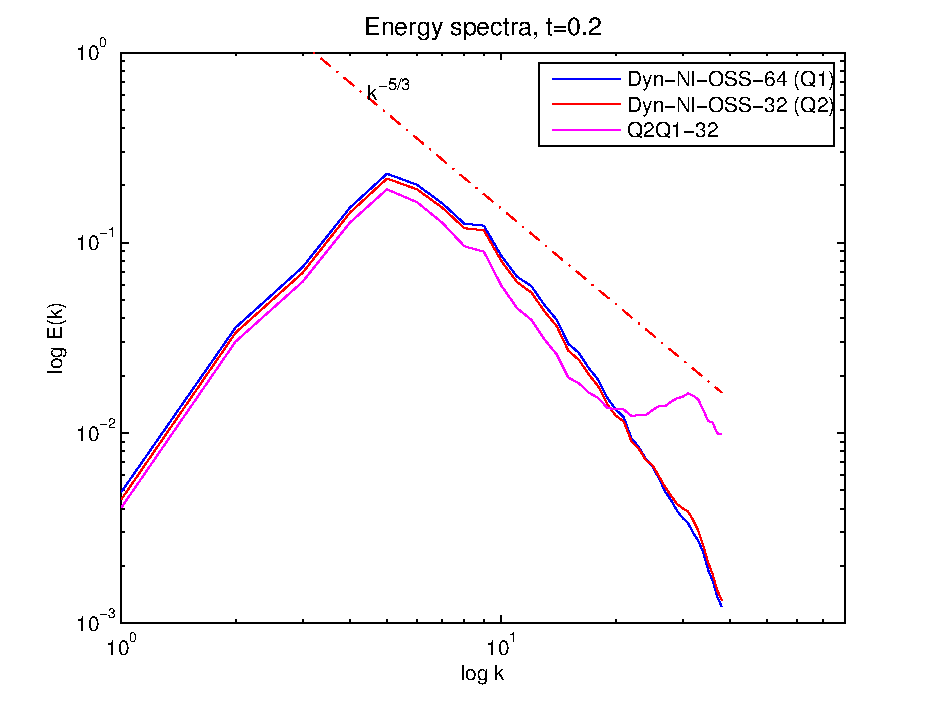
\includegraphics[width=0.49\textwidth]{Figures/DHIT/spec_q2q1_scaled_t02}}\\  
%   \subfigure[Energy spectra at $t=0.4$]{\label{fig:spec_q2q1_04}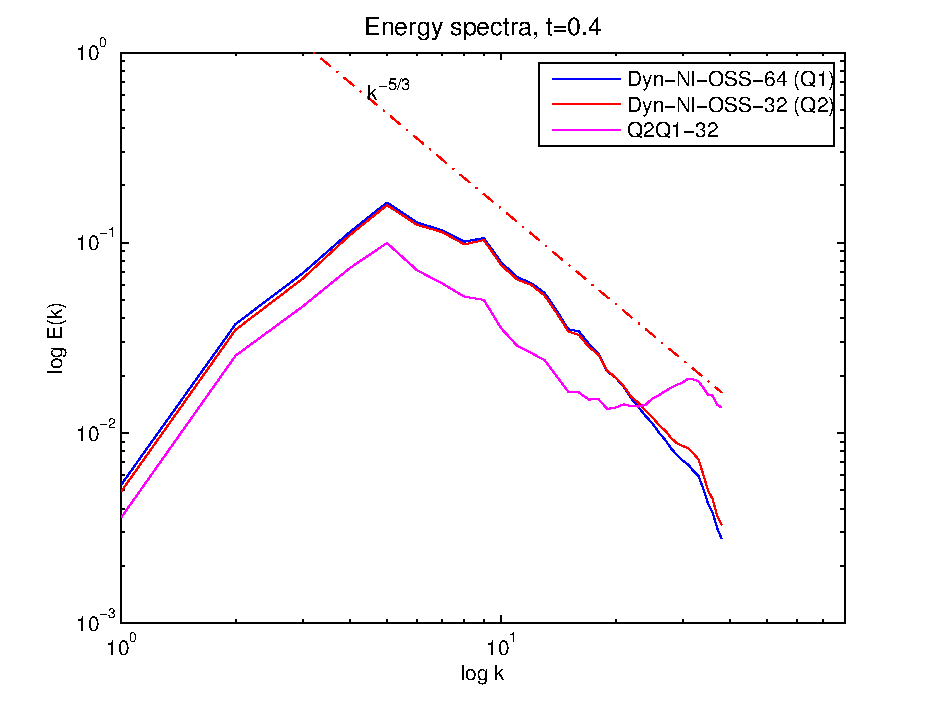
\includegraphics[width=0.49\textwidth]{Figures/DHIT/spec_q2q1_scaled_t04}}
%   \subfigure[Energy spectra at $t=0.8$]{\label{fig:spec_q2q1_08}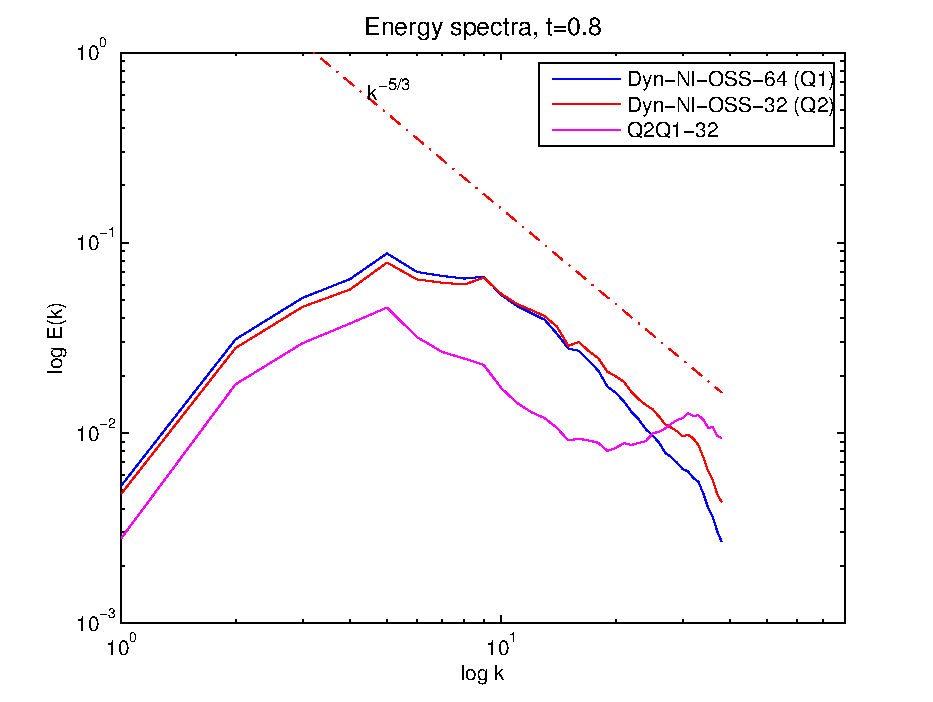
\includegraphics[width=0.49\textwidth]{Figures/DHIT/spec_q2q1_scaled_t08}}
%   \caption{Total kinetic energy evolution and energy spectra using OSS and non-stabilized method with an inf-sup stable $Q2/Q1$ element}
%   \label{fig:ene_spec_q2q1}
% \end{figure}

\subsection{Taylor-Green Vortex}
\label{subsec-C4_TGV}
This problem aims to show, in a relatively simple flow, the basic turbulence decay mechanisms like the turbulent energy cascade, the production of small eddies and the enhancement of dissipation by the stretching of vortex lines. We refer to Section \ref{sec-C3_TGV} for a deeper description of this problem.

The computational domain is the unit cube with periodical boundary conditions. The initial analytical condition is defined in the physical space (see, e.g., \cite{gassner_accuracy_????}), and given by
\begin{align}
\label{eq-C4_ini_sol_TG}
&u_x=u_0\cos(x)\sin(y)\sin(z),\\\nonumber
&u_y=-u_0\sin(x)\cos(y)\sin(z),\\\nonumber
&u_z=0,\\\nonumber
&p=p_0+\frac{1}{16}\left(\cos(2x)+\cos(2y)\right)\left(\cos(2z)+2\right),
\end{align}
with
$$u_0=\frac{2}{\sqrt{3}}\sin\left(\gamma+\frac{2\pi}{3}\right).$$
We choose $\gamma=0$, which gives the mean initial velocity  $u_0=1$. The pressure constant parameter $p_0$ is chosen equal to zero.

\subsubsection{Setting}

We solve the TGV problem using a Reynolds number ${\rm Re}=1600$. 
The most common Reynolds numbers available in the literature are ${\rm Re}=800$, ${\rm Re}=1600$ and ${\rm Re}=3000$ (see, e.g., \cite{andrea_d._beck_numerical_2012, fauconnier_construction_2009, gassner_accuracy_????, jb_chapelier_final_2012}).
We use the same VMS methods as for the DHIT problem defined in Section \ref{sec-C4_DHIT} to solve this test, namely the ASGS and OSS methods, both with linear and nonlinear definitions of the convective term and static or dynamic tracking in time of the subscales, as it is summarized in Table \ref{table:DHIT_cases}.
The stabilization parameters for each method are the same as those chosen for the DHIT test, see Subsection~\ref{subsubsec-C4_DHIT_setting}, and discussed in Section \ref{sec-C4_effect_const}.

Initially we consider a mesh of $32^3$ hexahedral linear elements $(Q_1)$, but we will redefine this discretization to analyze the method performance when we refine the mesh, decreasing the element size $h$ or increasing the degree of the interpolation polynomial $p$. It implies to solve the problem on meshes with $64^3$ and $128^3$ linear $(Q_1)$, quadratic $(Q_2)$ or cubic $(Q_3)$ hexahedral elements. We also use a $20^3(Q_3)$ discretization to compare against other authors results.

\subsubsection{Vorticity}
The TGV test is characterized by its laminar evolution at the initial time steps, when the flow is strongly anisotropic due to the structured large-scale vortices directly related to the initial condition. If the Reynolds number is large enough, the vortex-stretching process, which activates the energy cascade effect, transfers energy from large to small-scales and the flow becomes unstable and turbulent. According to Brachet \emph{et al.} \cite{brachet_small-scale_1983}, the flow becomes nearly isotropic for ${\rm Re}\geq1000$.

In Fig. \ref{fig:isovor_vel_TG} we present some vorticity isosurface images showing this process for  a $128^3$ linear hexahedral elements mesh, for the dynamic and nonlinear OSS method. Note that the initial condition (Fig. \ref{fig:isvor_vel_1}) consists in eight vortices with the same scale corresponding to the eight Fourier modes located at $\mathbf{k}=(\pm1,\pm1,\pm1)$, as it has been pointed out previously.

%\begin{figure}[h!]
%  \centering
%  \subfigure[Isosurface for $|\omega|=1.0$ at $t=0.0$]{\label{fig:isvor_vel_1}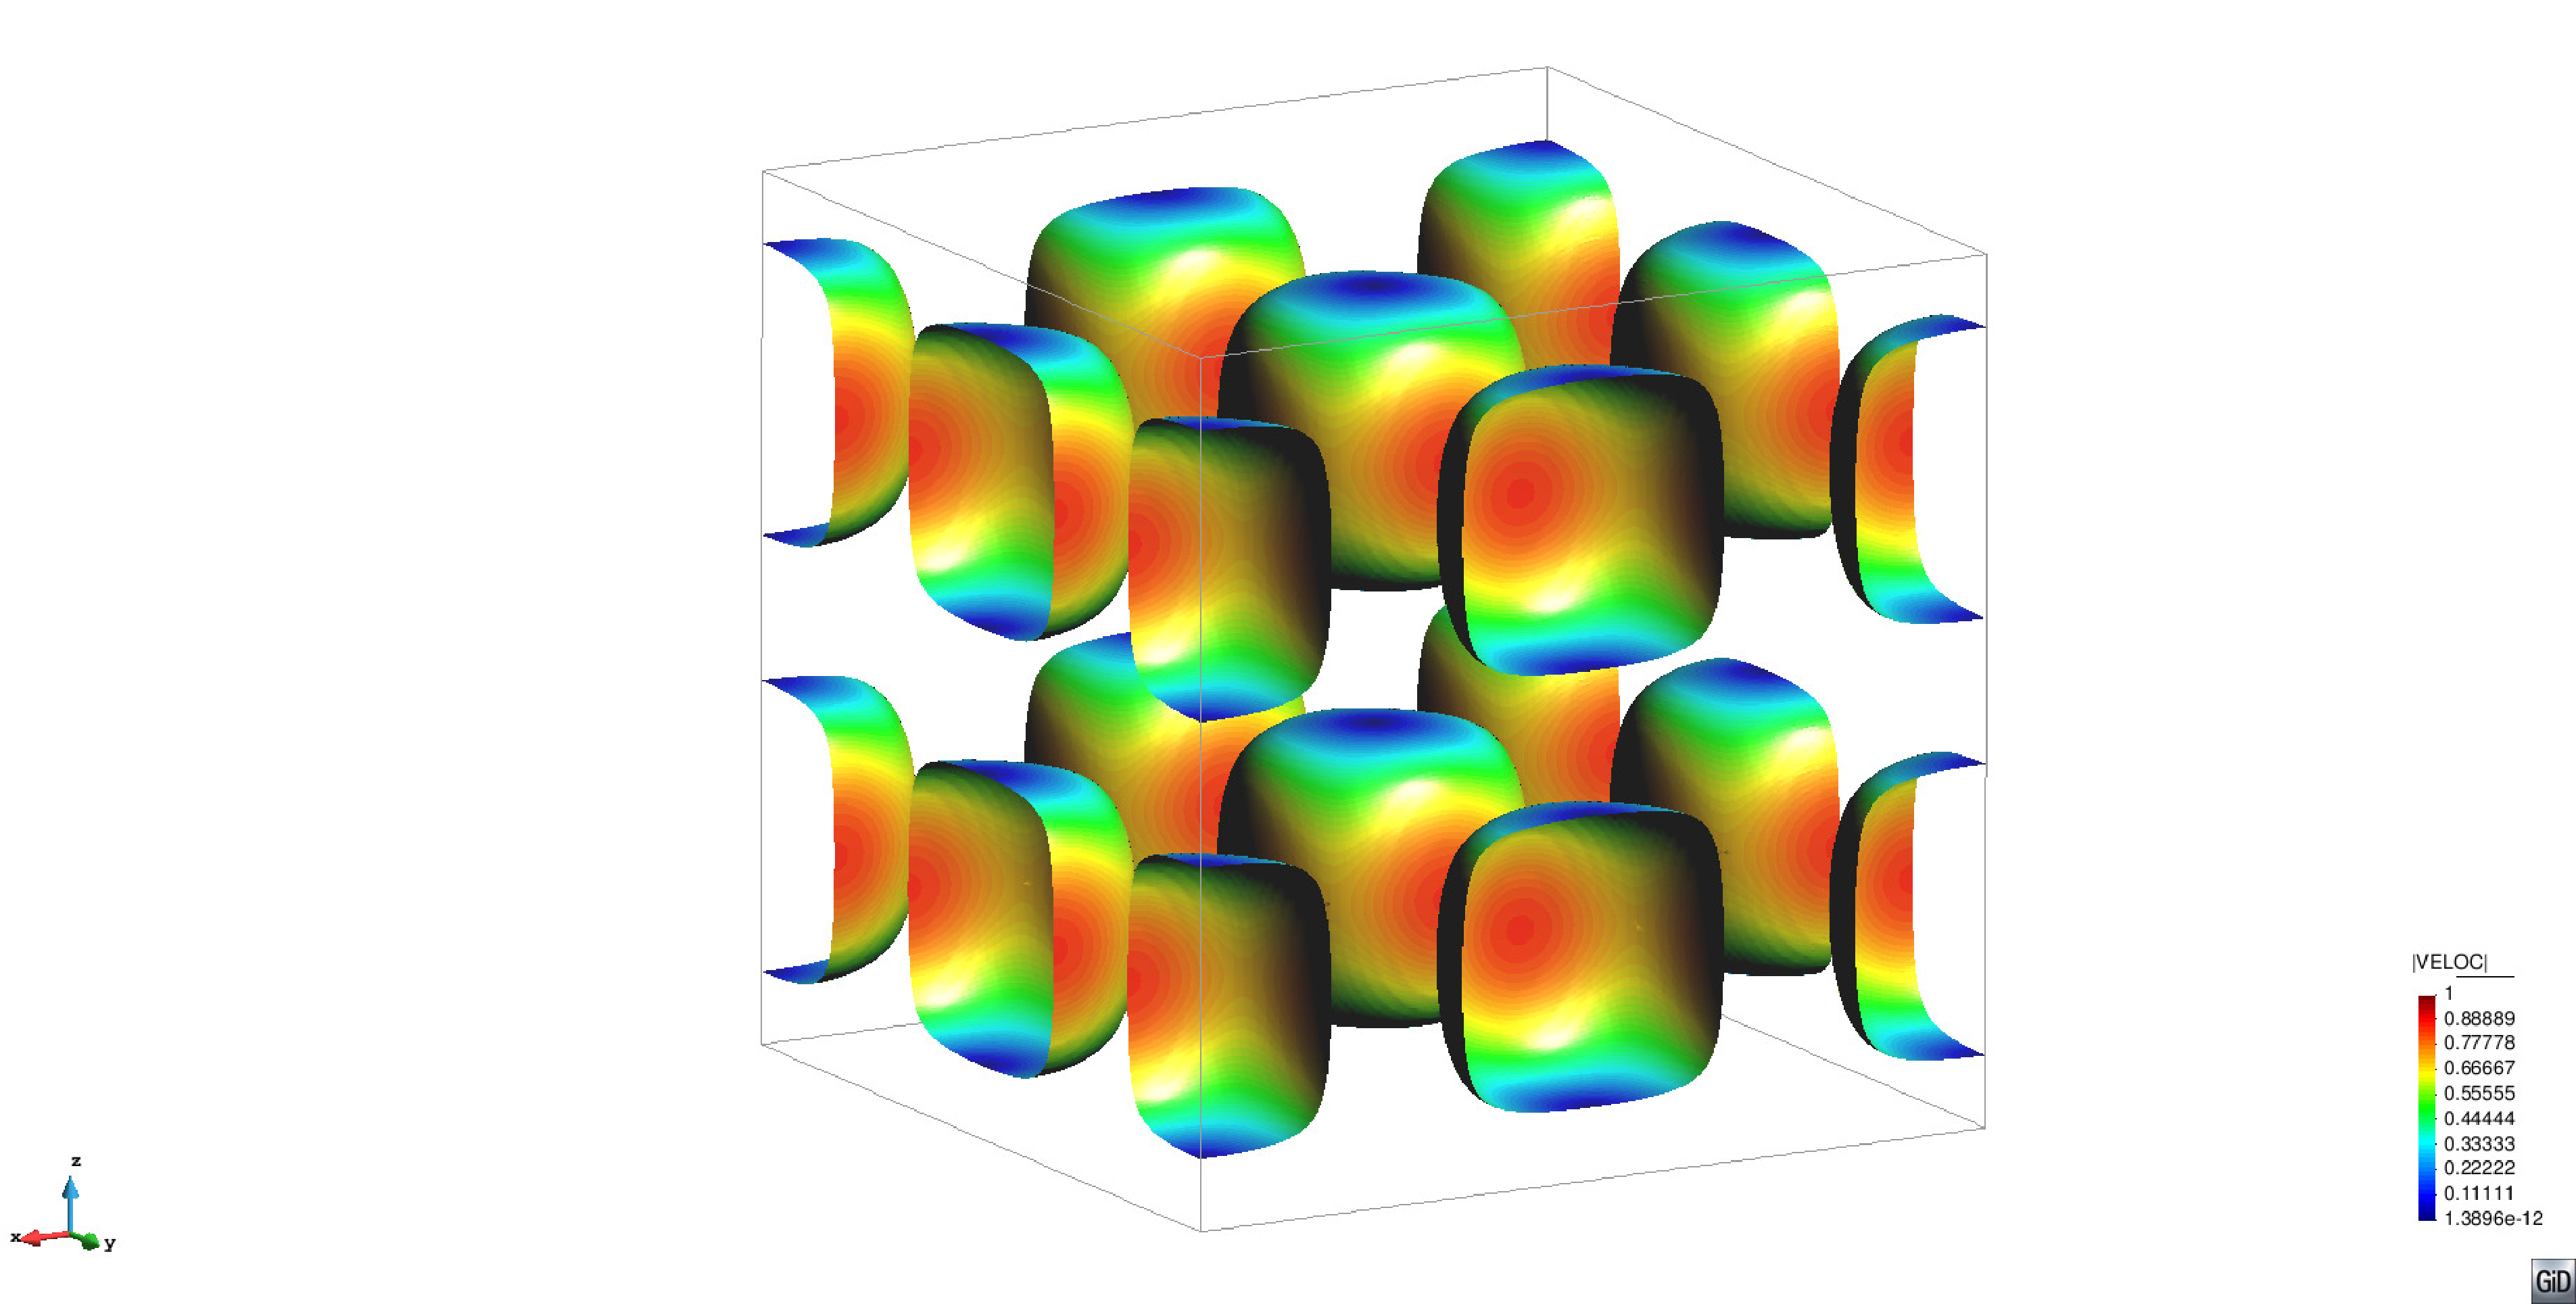
\includegraphics[clip=true, trim=13cm 0cm 13cm 0cm, width=0.45\textwidth]{Figures/TG/isovorti_veloc_1}}    
%  \subfigure[Isosurface for $|\omega|=1.0$ at $t=2.0$]{\label{fig:isvor_vel_2}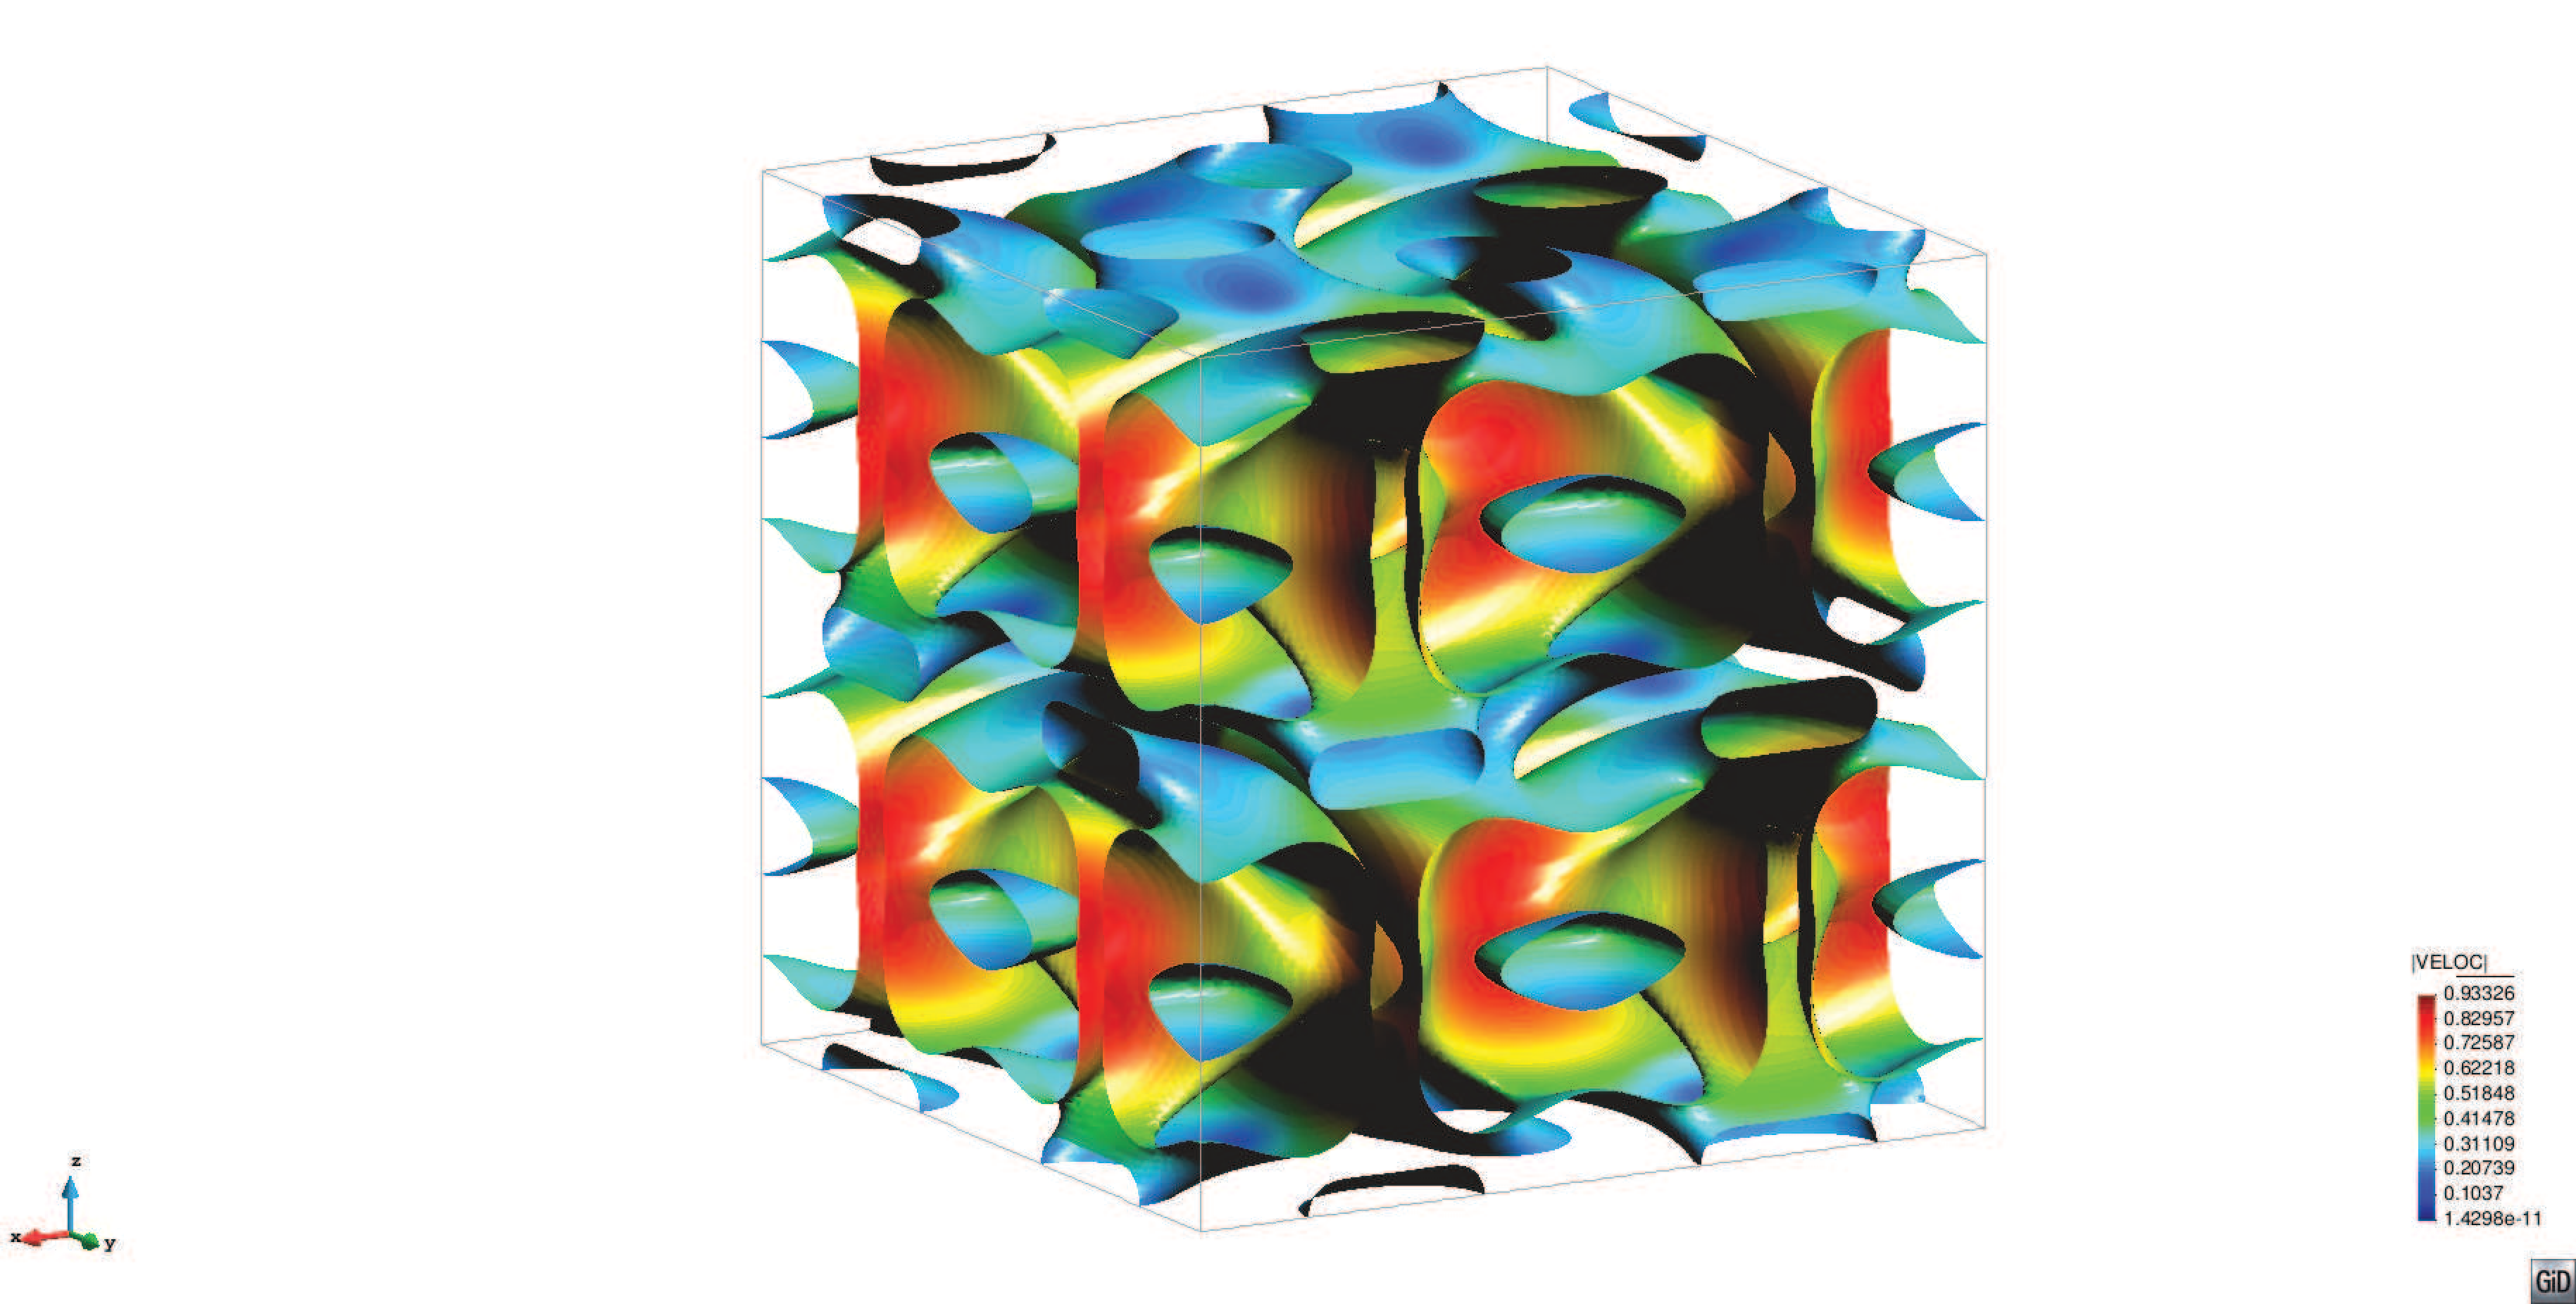
\includegraphics[clip=true, trim=13cm 0cm 13cm 0cm, width=0.45\textwidth]{Figures/TG/isovorti_veloc_2}}\\
%    \centering
%  \subfigure[Isosurface for $|\omega|=2.5$ at $t=4.1$]{\label{fig:isvor_vel_3}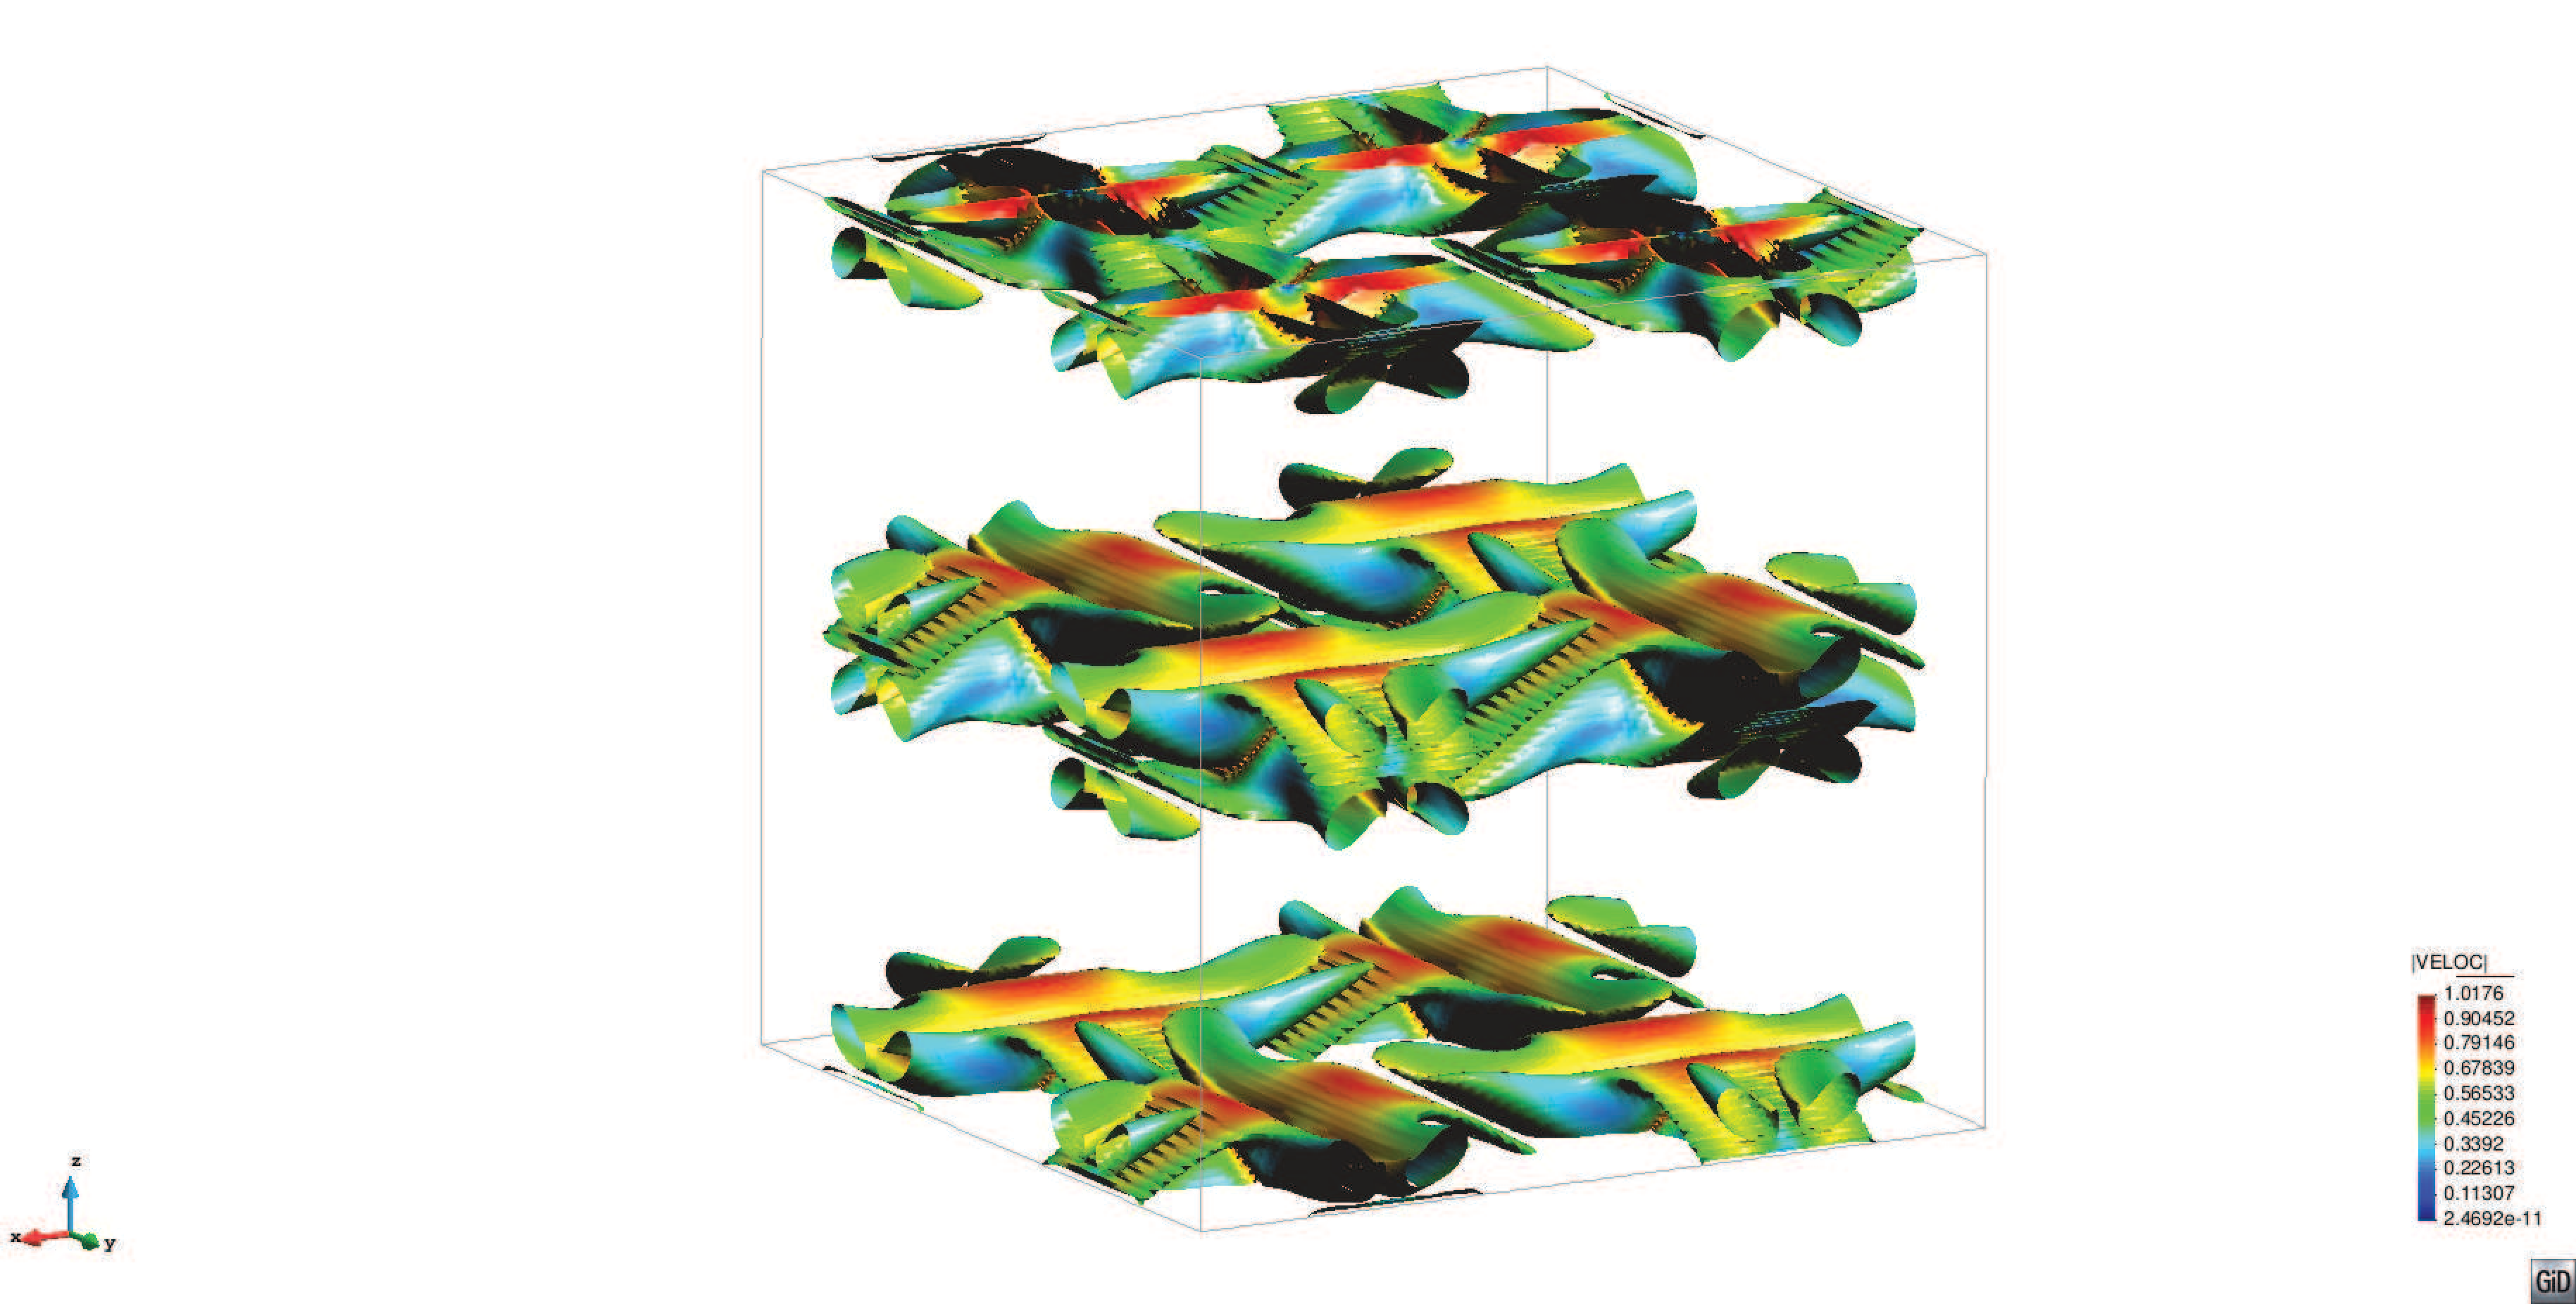
\includegraphics[clip=true, trim=13cm 0cm 13cm 0cm, width=0.45\textwidth]{Figures/TG/isovorti_veloc_3}}    
%  \subfigure[Isosurface for $|\omega|=5.0$ at $t=6.1$]{\label{fig:isvor_vel_4}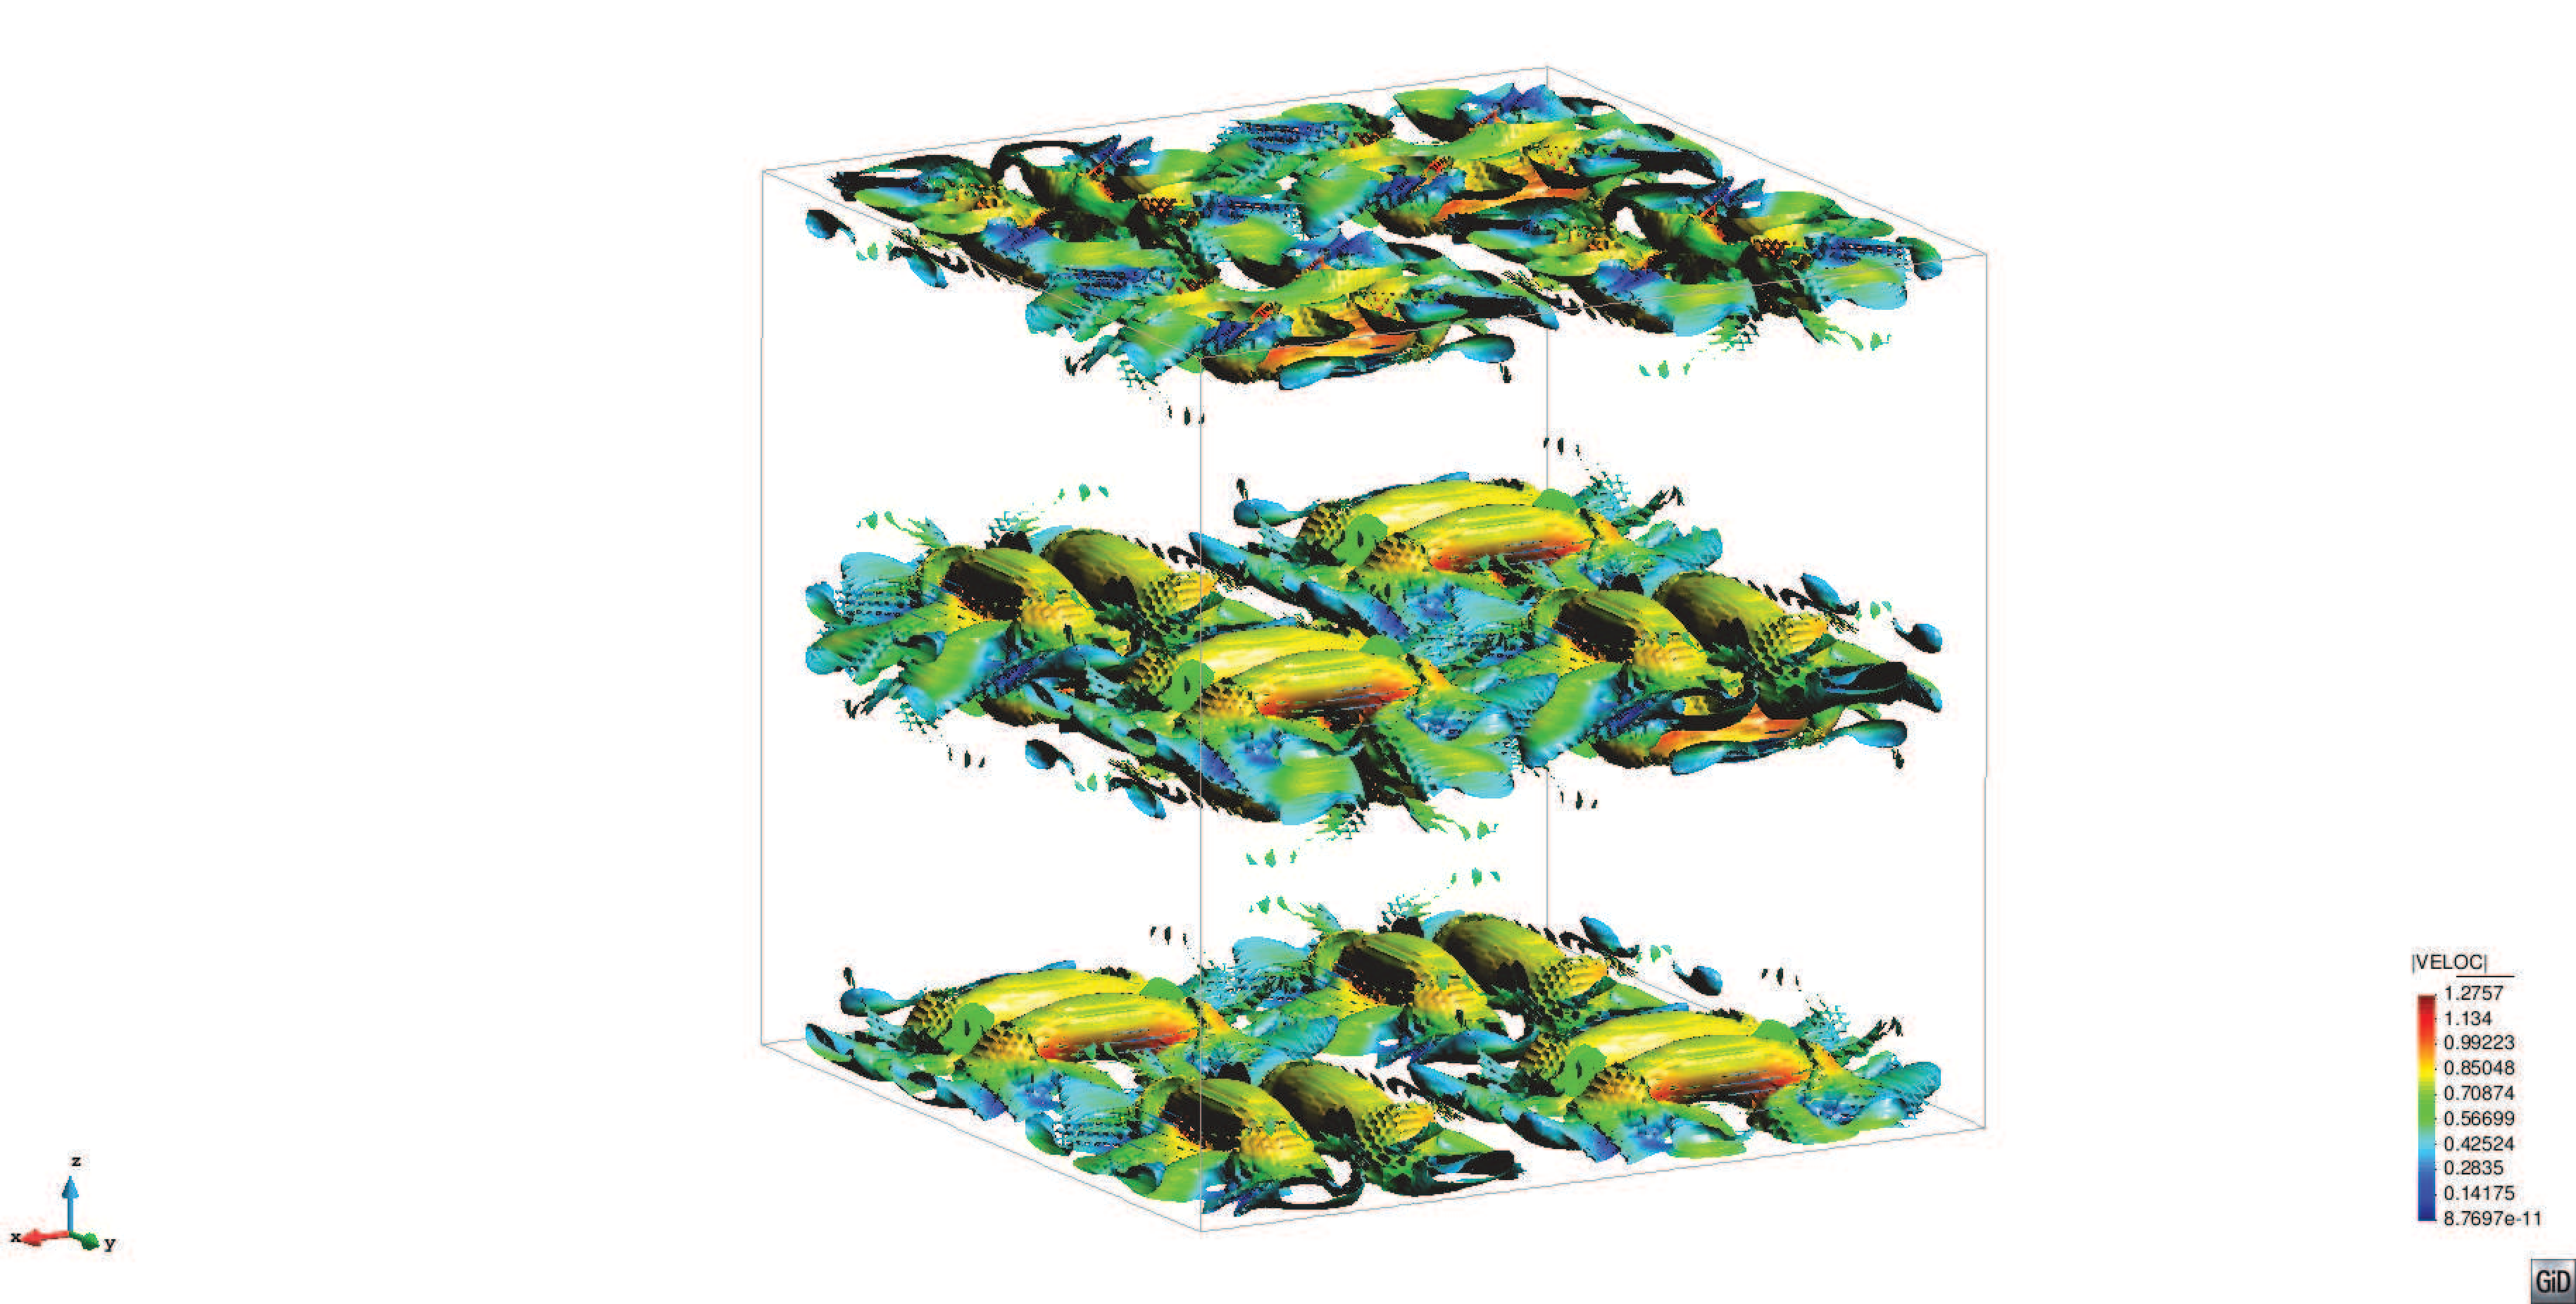
\includegraphics[clip=true, trim=13cm 0cm 13cm 0cm, width=0.45\textwidth]{Figures/TG/isovorti_veloc_4}}\\
%    \centering
%  \subfigure[Isosurface for $|\omega|=8.0$ at $t=8.2$]{\label{fig:isvor_vel_5}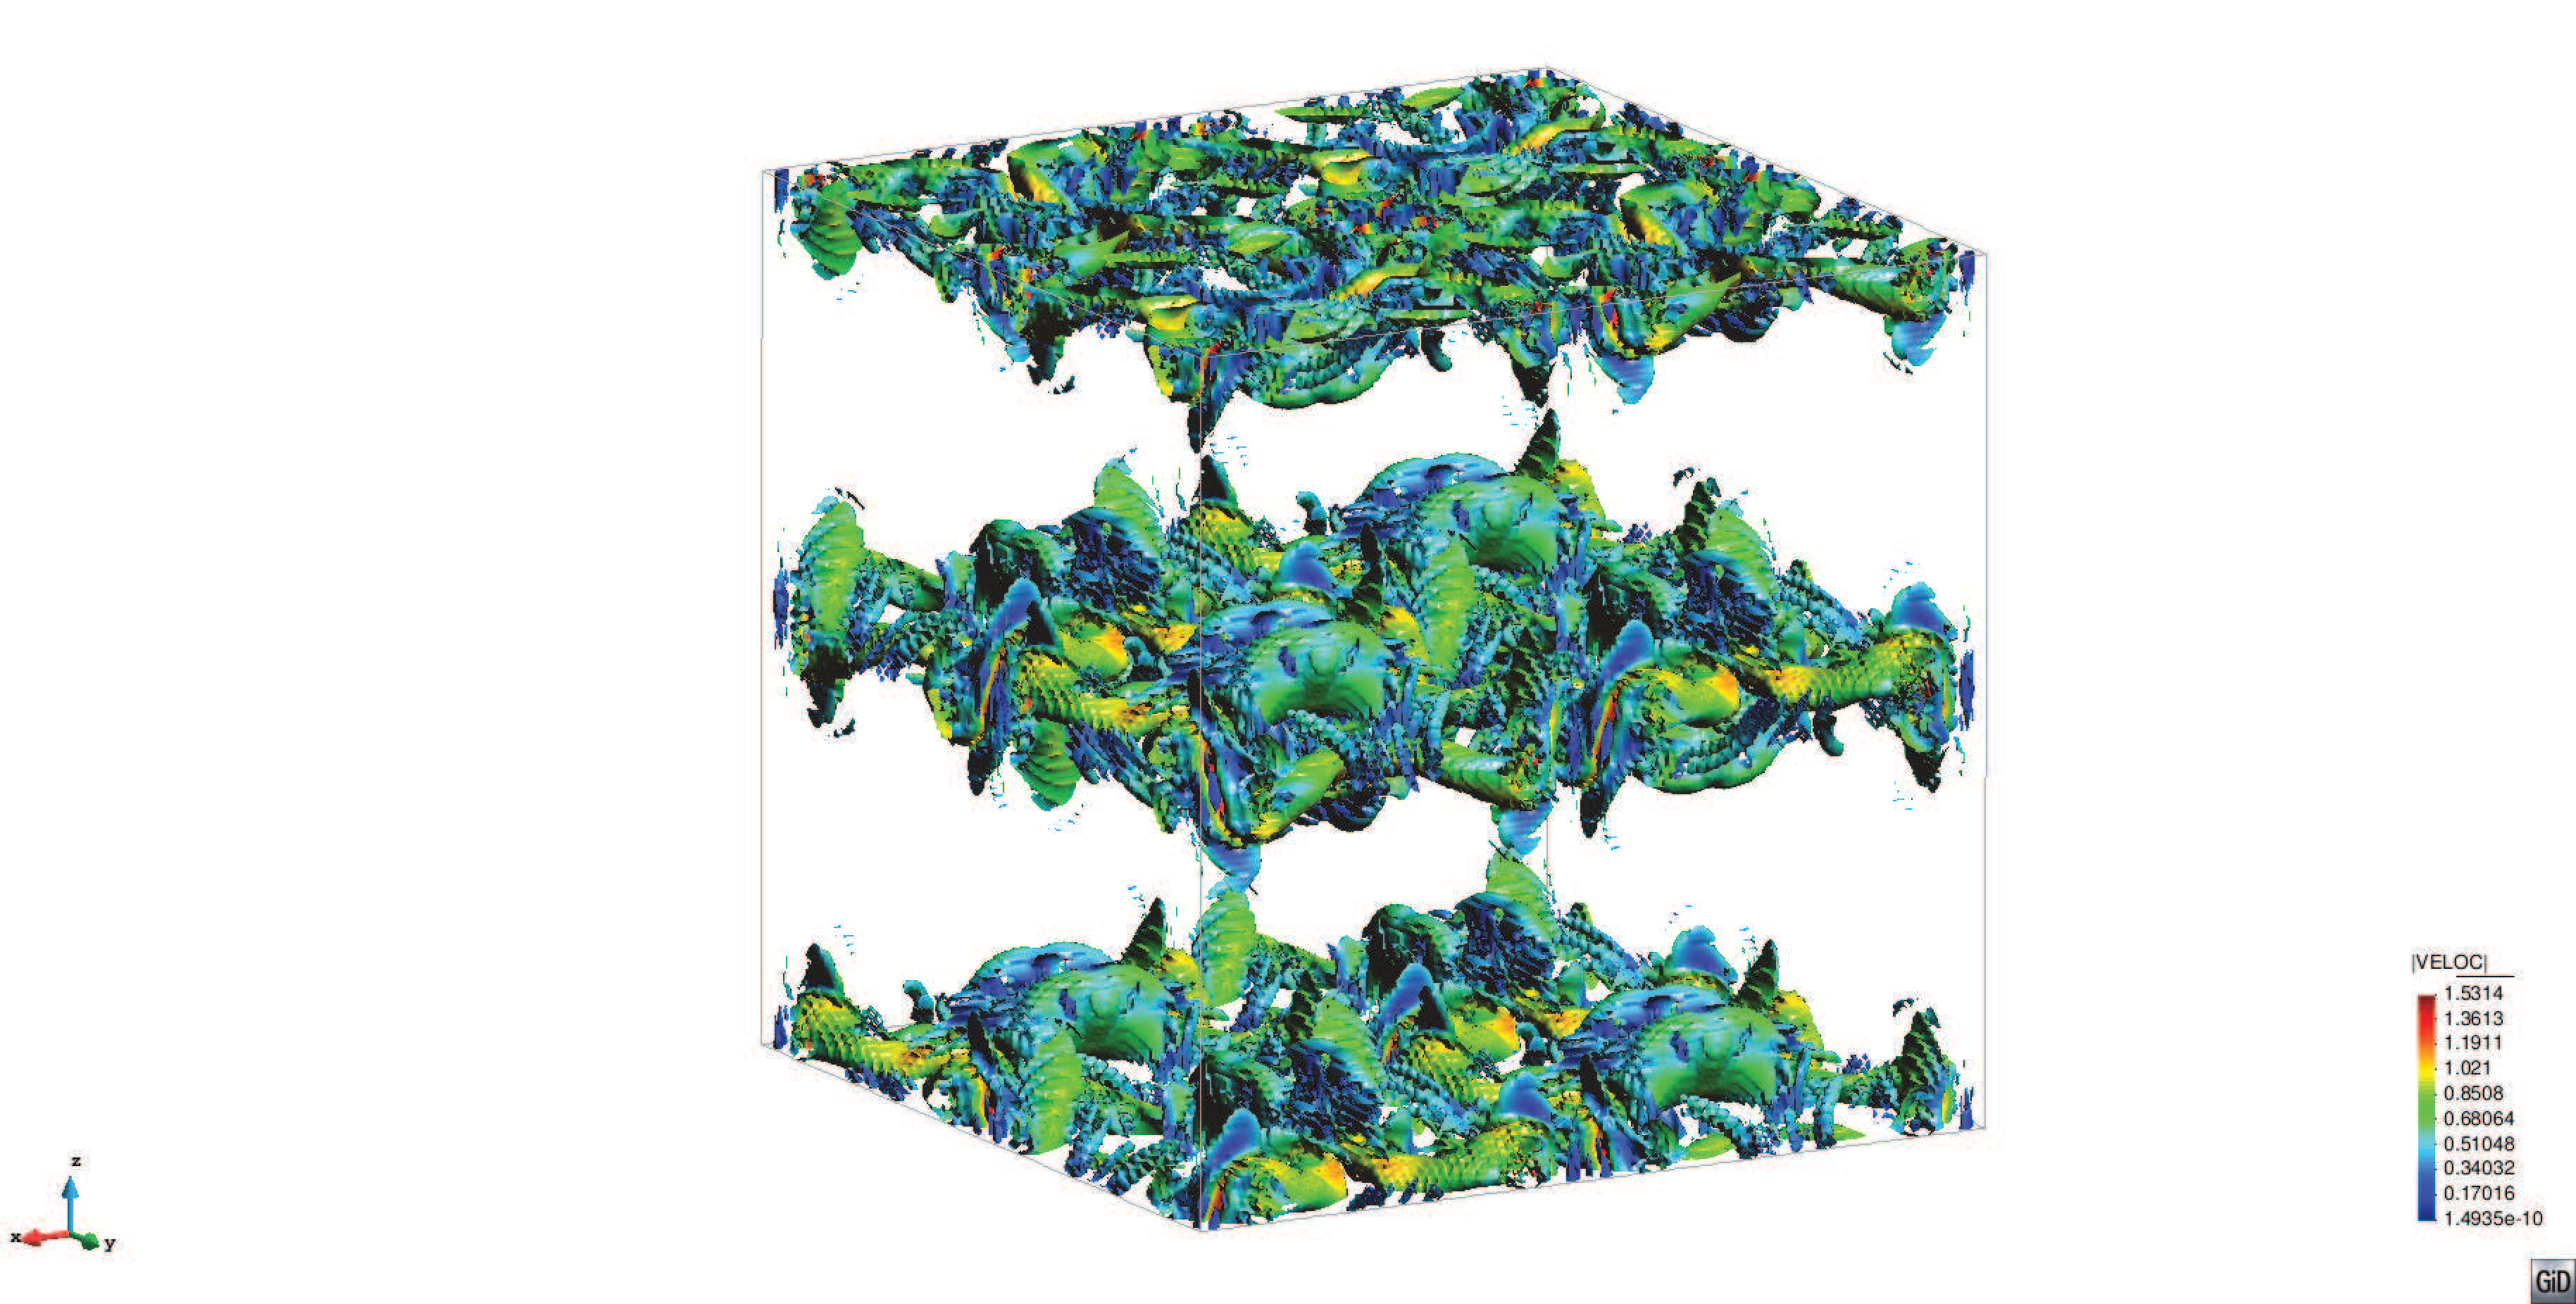
\includegraphics[clip=true, trim=13cm 0cm 13cm 0cm, width=0.45\textwidth]{Figures/TG/isovorti_veloc_5}}    
%  \subfigure[Isosurface for $|\omega|=9.0$ at $t=10.2$]{\label{fig:isvor_vel_6}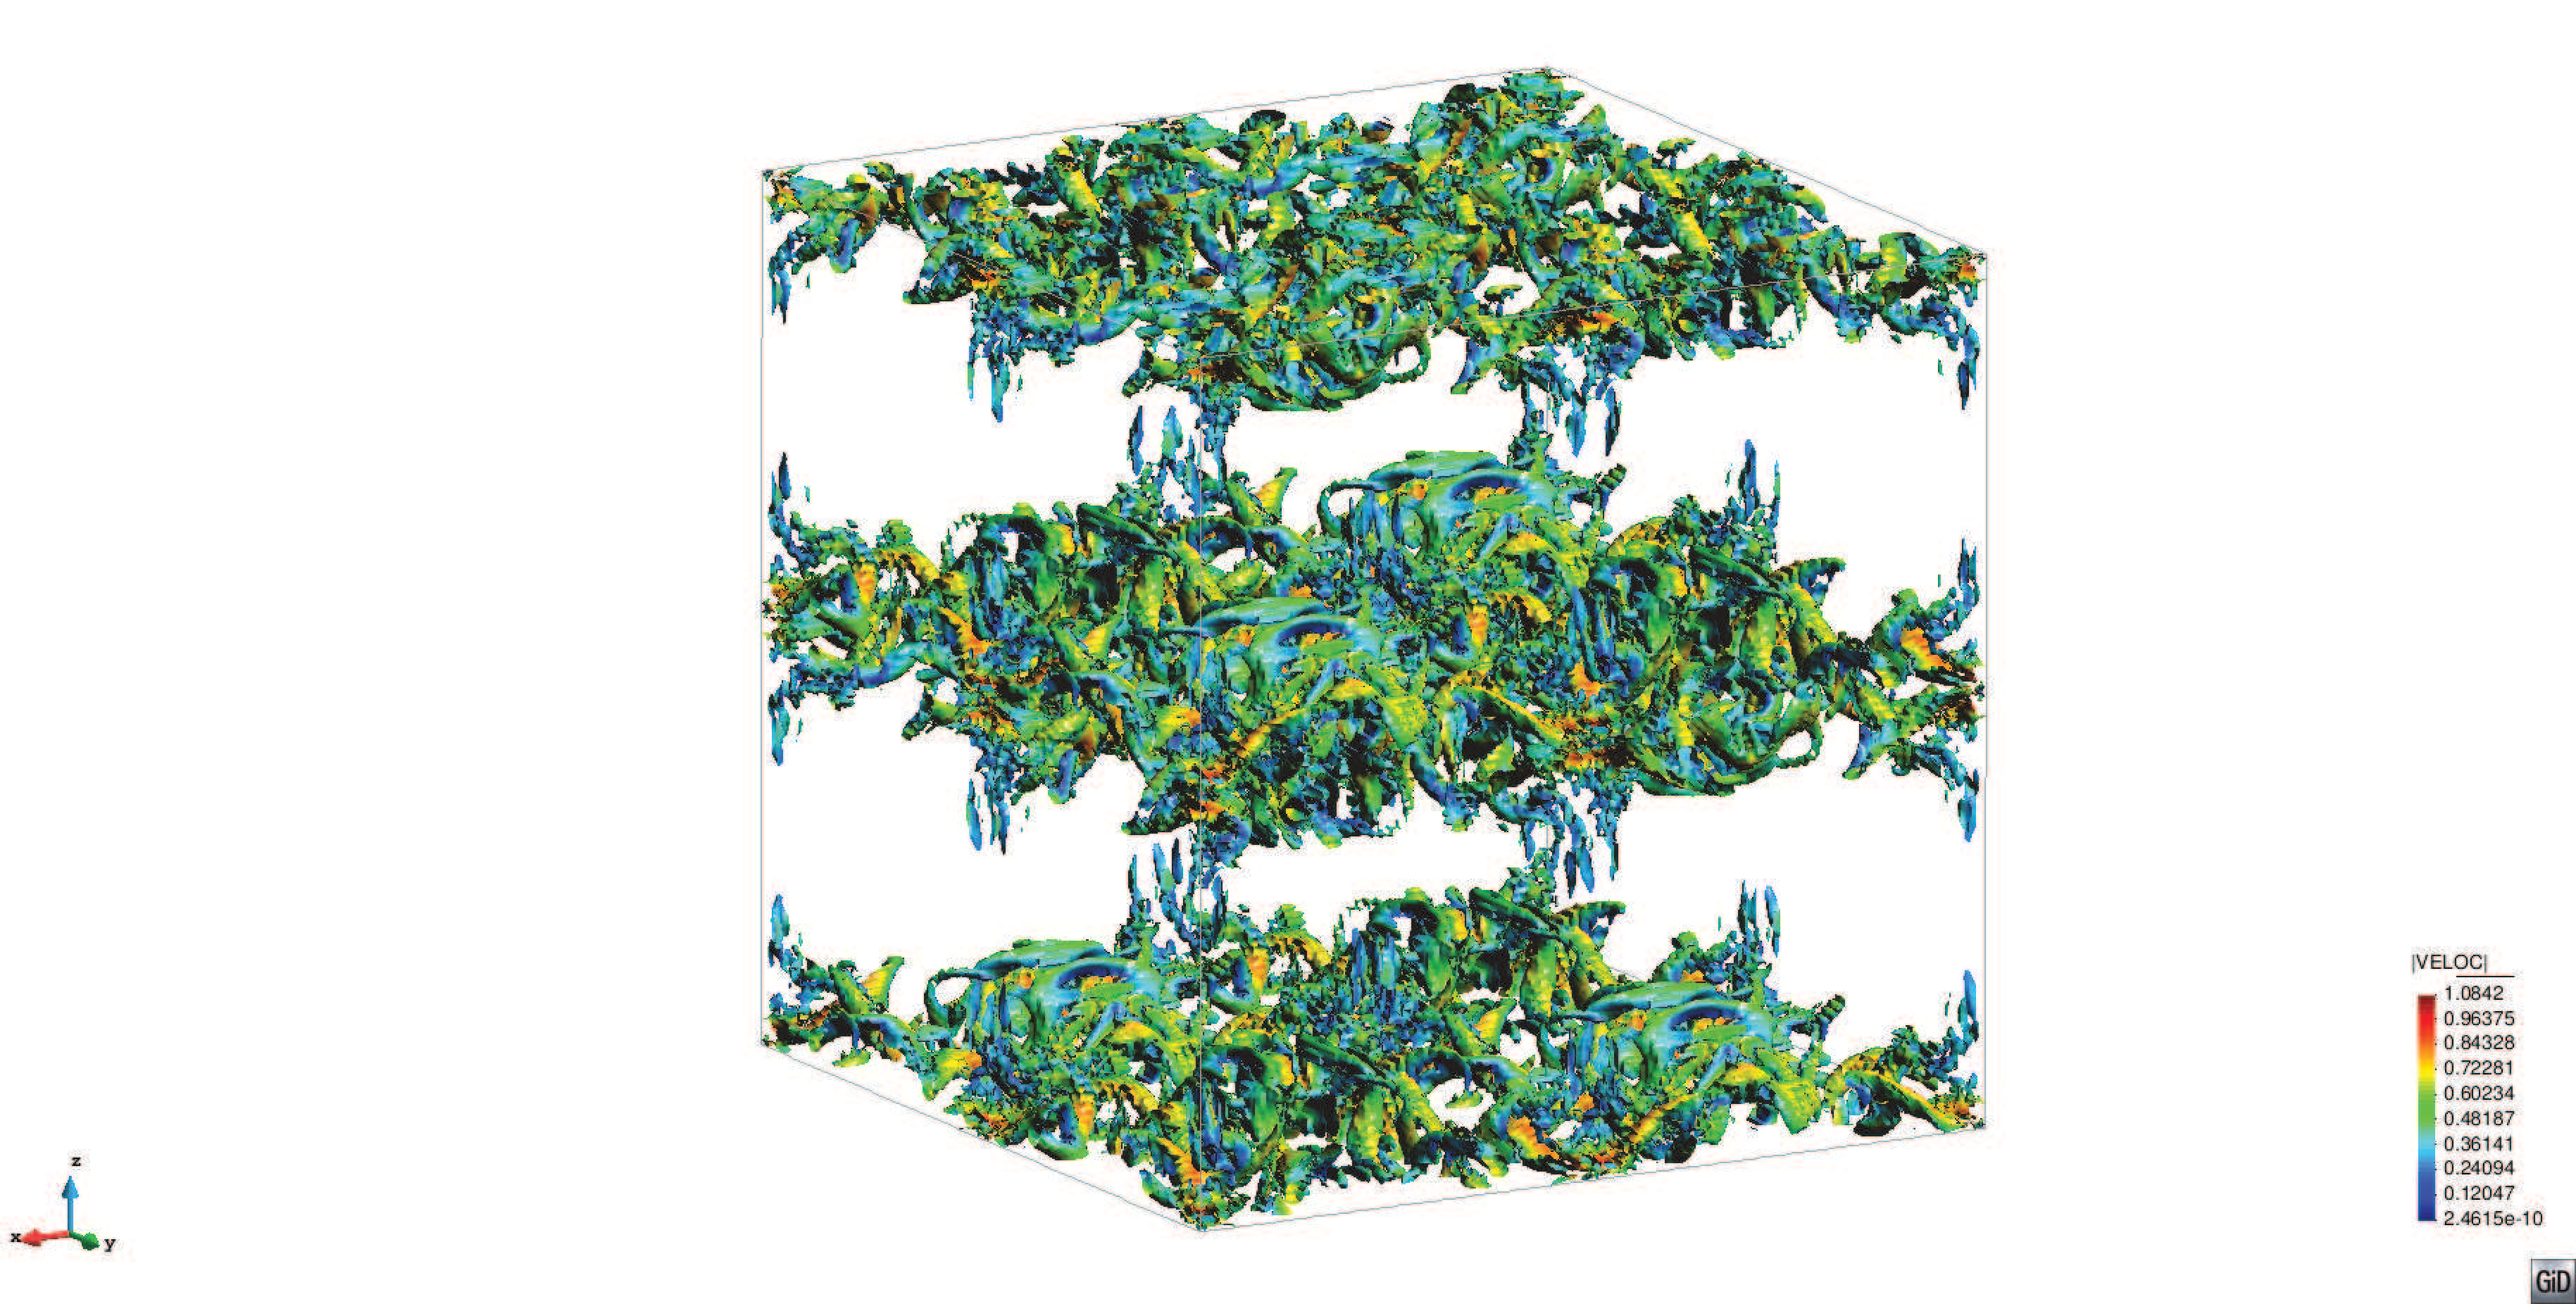
\includegraphics[clip=true, trim=13cm 0cm 13cm 0cm, width=0.45\textwidth]{Figures/TG/isovorti_veloc_6}}\\
%  \caption{Vorticity isosurfaces with velocity contour at different time steps.}
%  \label{fig:isovor_vel_TG}
%\end{figure}
%
%%\begin{figure}[h!]
%%	\centering	
%%	\includegraphics[clip=true, trim=13cm 0cm 13cm 0cm, width=0.5\textwidth]{Figures/TG/isovorti_streaml_veloc_1}
%%	\caption{Vorticity isosurfaces at $t=4.0$ with streamlines}
%%	\label{fig:vorti_stream_TG}
%%\end{figure}

\subsubsection{Comparison of VMS methods}

In order to compare the different VMS methods defined previously and to test their performance as LES models
%see if they can be considered LES models, 
we solve the TGV test on a $32^3$ and $64^3$ linear elements mesh with a Reynolds number ${\rm Re}=1600$. 

We want to show the amount of numerical dissipation, the energy cascade in the spectra and the enstrophy evolution (compared to DNS) in all cases. We compare first the kinetic energy evolution  with the kinetic energy evolution obtained by Brachet \emph{et al.} \cite{brachet_small-scale_1983}, (Fig. \ref{fig:ene_32_TG}). We also present the energy spectra at $t=9$, when the flow is supposed to be nearly isotropic at large wave numbers, (Fig. \ref{fig:spec_32_TG}).

%  \begin{figure}[h!]
% 	\centering	
% 	\subfigure[Total kinetic energy evolution]{\label{fig:ene_32_TG}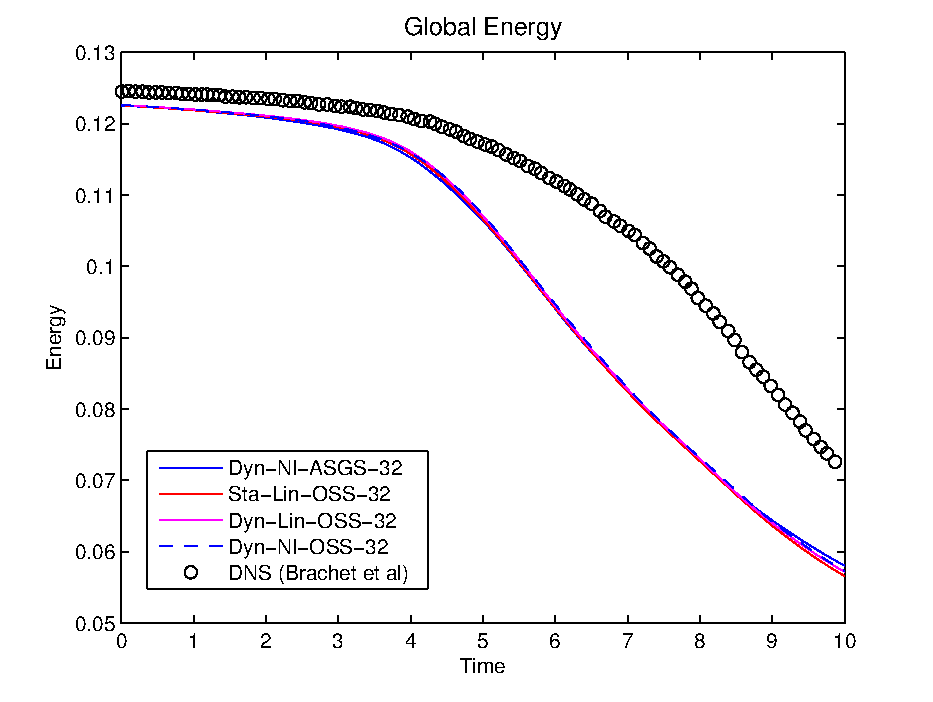
\includegraphics[width=0.4\textwidth]{Figures/TG/ene_32_new}}
% 	\subfigure[Energy spectra at $t=9.0$]{\label{fig:spec_32_TG}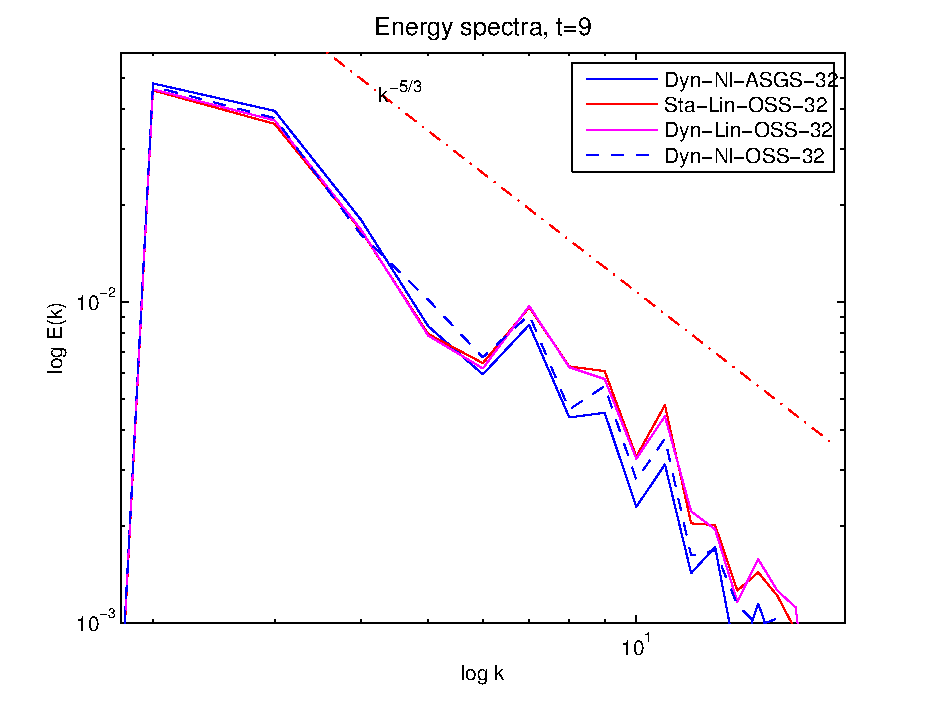
\includegraphics[width=0.4\textwidth]{Figures/TG/spec_32_x2_new}}
% 	\caption{Total kinetic energy evolution and energy spectra}
% 	\label{fig:ene_spec_32_TG}
% \end{figure}

In Fig. \ref{fig:ene_32_TG}, we can see that for a $32^3$ trilinear hexahedral elements mesh all methods show a premature decay of energy. We recognize the same behavior observed for the same mesh in the DHIT test, see Subsection \ref{subsubsec-C4_Total_ene_DHIT}. For this mesh, it is clear that the methods are not able to simulate properly the transition to turbulence. The energy spectra at $t=9.0$ shows us that the flow is isotropic at large wave numbers since it is decaying following the $k^{-5/3}$ Kolmogorov law. 

As in the DHIT test, the cases with nonlinear and dynamic definitions of the subscales, using either ASGS or OSS methods, seem to be slightly less dissipative. Furthermore, OSS is a little bit less dissipative than ASGS, but the differences are not important. 

As for the DHIT test, the results obtained using the different methods listed in Table \ref{table:DHIT_cases} are very similar for these coarser discretizations. The only point that is worth to note is that the linear and static ASGS case (Sta-Lin-ASGS) and the dynamic and linear ASGS case (Dyn-Lin-ASGS) diverge at some time step before $t=9$. Anyway, all the methods converge as $h\rightarrow0$ and the accuracy depends much more on the mesh size than on the choice of the method. In turn, similar trends for the computational cost analyzed in the previous section have been observed.

\subsubsection{$h$-$p$ refinement}

As in the DHIT problem, we perform a refinement study reducing $h$ and/or increasing $p$ using  Dyn-Nl-OSS. 
The global energy evolution and the energy spectra are shown in Fig. \ref{fig:ene_spec_hp_TG}. Fig. \ref{fig:ene_hp_TG} displays the total kinetic energy evolution compared with the DNS \cite{brachet_small-scale_1983}. The results show that all cases, excluding the $32^3$ and $64^3$ linear hexahedral mesh, follow almost perfectly the line defined by the DNS result points. On the other hand, Fig. \ref{fig:spec_hp_TG} displays the energy spectra at $t=9$, when the dissipation is maximum and the flow is evolving to turbulence. We compare the energy spectra obtained solving all the cases considered before with the DNS computed by \cite{gassner_accuracy_????}, using the same Reynolds number (${\rm Re}=1600$) at the same time. 

% \begin{figure}[h!]
% 	\centering
%	\subfigure[Total kinetic energy evolution]{\label{fig:ene_hp_TG}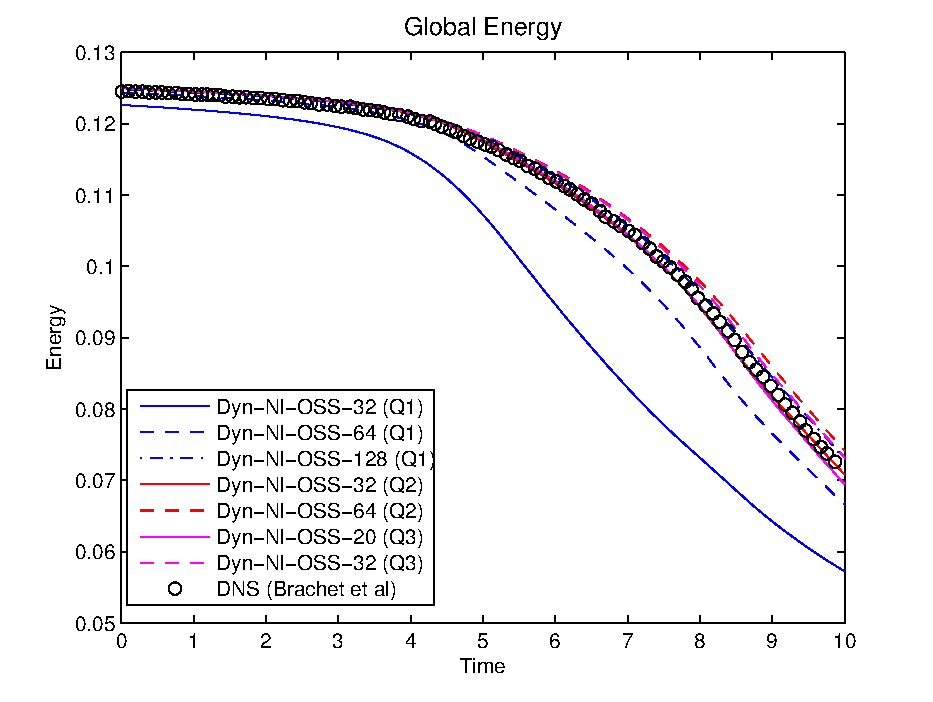
\includegraphics[width=0.49\textwidth]{Figures/TG/ene_hp_10_new}}
%	\subfigure[Energy spectra at $t=9$]{\label{fig:spec_hp_TG}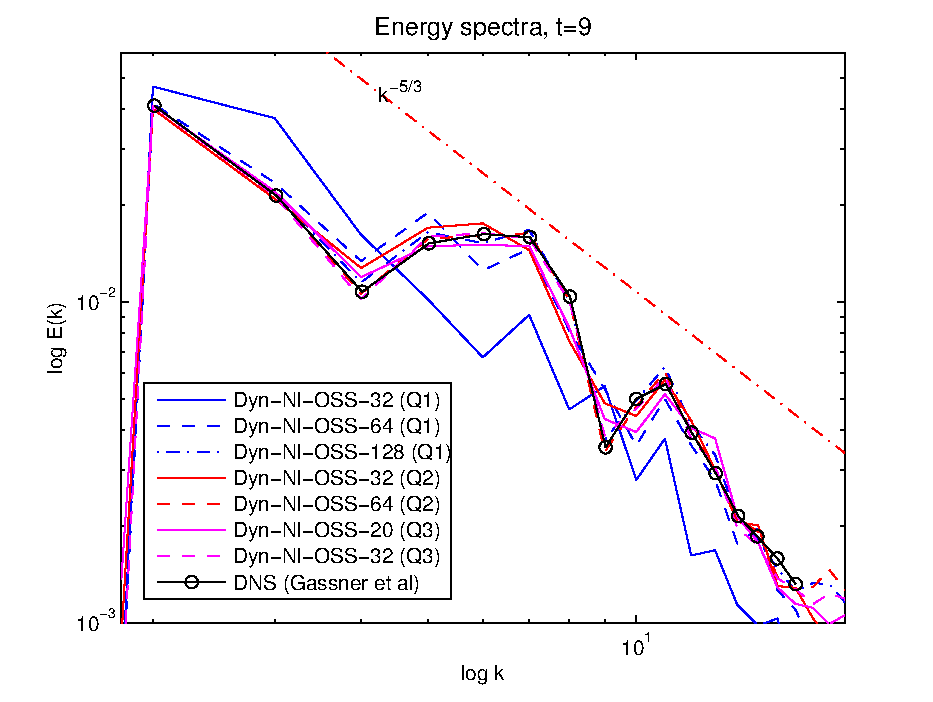
\includegraphics[width=0.49\textwidth]{Figures/TG/spec_hp_x2_new}}
% 	\caption{Total kinetic energy evolution and energy spectra for the $h-p$ refinement cases.}
% 	\label{fig:ene_spec_hp_TG}
% \end{figure}

% Excluding the too coarse $32^3 (Q1)$ approximation, the energy spectra follow accurately the DNS energy spectra. For low wave numbers, the differences with the DNS are minimal. It is on the highest wave numbers where some differences between the methods appear. Note that the $32^3(Q3)$ case follows very accurately the DNS spectrum. In general, we see that the spectra decay following a slope close to the $k^{-5/3}$ Kolmogorov law.
% %Anyway, we must emphasize that the flow is supposed to be isotropic after $t=9$, so we expect that this slope becomes closer to the predicted by Kolmogorov.

In Fig. \ref{fig:enediss_hp_TG} we show the dissipation rate of the problem, compared to the DNS results. The dissipation rate is directly related to the enstrophy of the problem, $\epsilon = 2\nu\left(\frac{1}{2}\left\langle|\omega|^2\right\rangle\right)$, where $|\omega|$ is the modulus of the vorticity. At the continuous level, it determines the kinetic energy decay which, at the discrete level, is also influenced by the numerical dissipation (see equation (\ref{eq-C4_FE_balance2})). When an explicit model is used, the dissipation introduced by the subgrid model also needs to be included. The FE viscous dissipation $\nu\|\nabla\u_h\|^2$, is shown in Fig. \ref{fig:enediss_hp_TG_resolved} whereas the total dissipation rate $ \nu\|\nabla\u_h\|^2 + \varepsilon_{h}$ defined by equation (\ref{eq-C4_FE_balance2}) is shown in Fig. \ref{fig:enediss_hp_TG_total}. 

%Fig. \ref{fig:ene_hp_TG} displays the total kinetic energy dissipation rate evolution for all the cases defined in Table \ref{table:refinement}, compared with the DNS \cite{brachet_small-scale_1983}. The results show that all cases, excluding the $32^3$ linear hexahedral mesh, follow almost perfectly the line defined by the DNS result points.

%\begin{figure}[h!]
%	\centering	
%	\subfigure[Resolved]{\label{fig:enediss_hp_TG_resolved}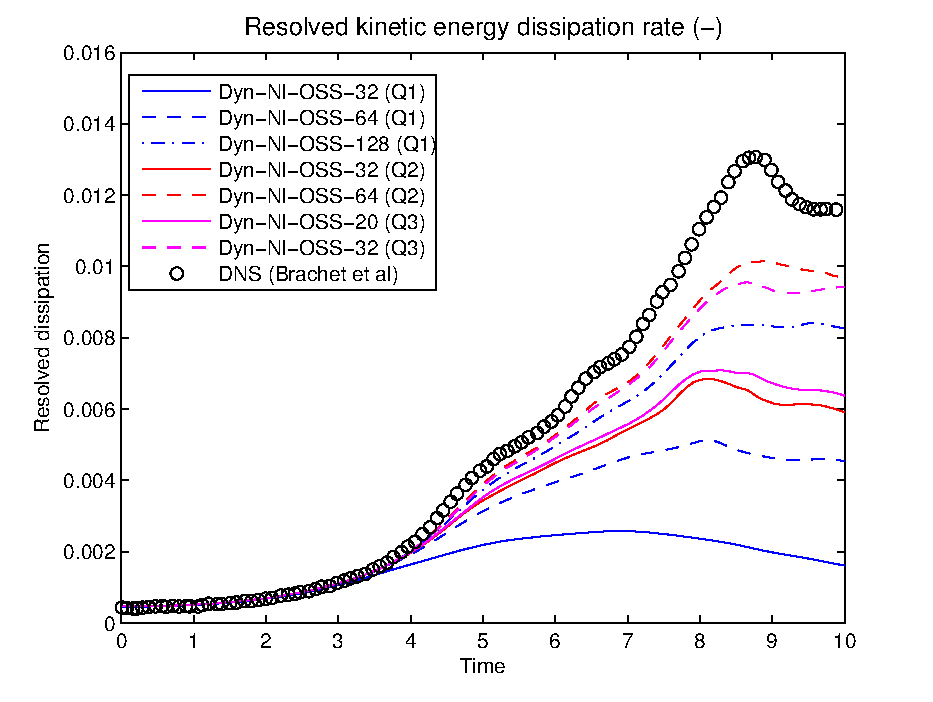
\includegraphics[width=0.49\textwidth]{Figures/TG/ens_hp_10_new_resolved}}
%	\subfigure[Total]{\label{fig:enediss_hp_TG_total}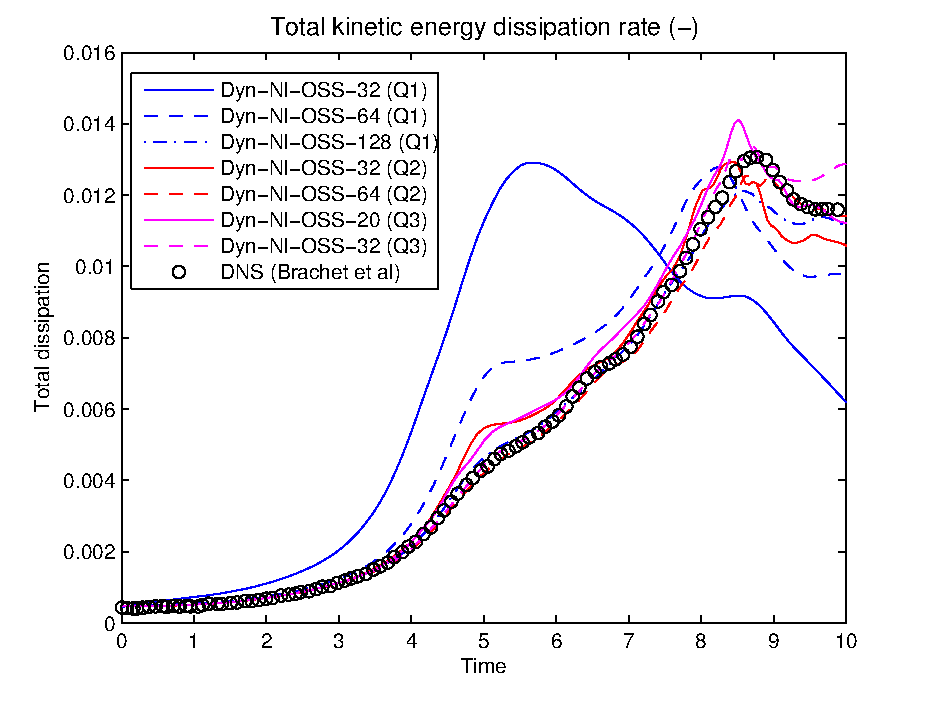
\includegraphics[width=0.49\textwidth]{Figures/TG/ens_hp_10_new_total}}
%	\caption{Dissipation rate evolution for the $h$-$p$ refinement cases.}
%	\label{fig:enediss_hp_TG}
%\end{figure}

As in the DHIT problem, the results obtained using the coarser $32^3 (Q1)$ and $64^3 (Q1)$ meshes are not accurate, the FE viscous dissipation being far from the exact viscous dissipation, as shown in Fig. \ref{fig:enediss_hp_TG_resolved}. The total dissipation introduced by the method is too large and, especially for the $32^3 (Q1)$, peaked at earlier times, i.e., the energy decays faster and earlier than it should (see Fig. \ref{fig:enediss_hp_TG_total}). When finer resolutions are used, the flows dynamics are much better predicted. Even when the resolution is not enough to completely capture the viscous dissipation, the total dissipation compares very well with the exact one, as shown in  Fig. \ref{fig:enediss_hp_TG}. This is a \emph{clear illustration of the very good performance of the method, which adds the right amount of dissipation when the gradients are not captured by the resolution.}

\subsubsection{Comparison with a non-stabilized method}

All the results presented up to this point have been computed using a VMS method, either ASGS or OSS. But, what would be the result using other methods? Are the methods presented here, comparable to classical LES methods? Which methods perform better? To answer all these questions, we compare the results obtained here against those obtained using the dynamic Smagorinsky model \cite{fauconnier_construction_2009} and the adaptive local deconvolution method \cite{hickel_adaptive_2006} specifically designed as an implicit LES model. The former has been obtained with a filter of size $2 \pi / 64$ and spectral resolution up to $2 \pi / 256$, thus not having numerical but only modeling error. In turn, the latter has been obtained using a $64^3$ grid without explicit subgrid model, an explicit third-order Runge-Kutta scheme for the time discretization, a fourth order spatial approximation of the symmetric terms and its particular approximation of the convective term which is based on the (forth order) five-point central stencils approximation of the convective term \cite{hickel_adaptive_2006}. To make the comparison as fair as possible we select those combinations of $h$ and $p$ that result in a similar number of degrees of freedom, which are $64^3 (Q1)$ (second order), $32^3 (Q2)$ (third order) and $20 (Q3)$ (fourth order) meshes (the last one having actually a bit less degrees of freedom).

The FE viscous dissipation is shown in Fig. \ref{fig:enediss_dynsmag_resolved} compared to the resolved dissipation obtained using the dynamic Smagorinsky model \cite{fauconnier_construction_2009} and the ``molecular dissipation'' of \cite{hickel_adaptive_2006} (the one computed using the molecular viscosity and the approximated solution, equivalent to our FE viscous dissipation but in the finite volume context). The total dissipations of the three methods are compared in Fig. \ref{fig:enediss_dynsmag_total}. 

%\begin{figure}[h!]
%	\centering	
%	\subfigure[Resolved]{\label{fig:enediss_dynsmag_resolved}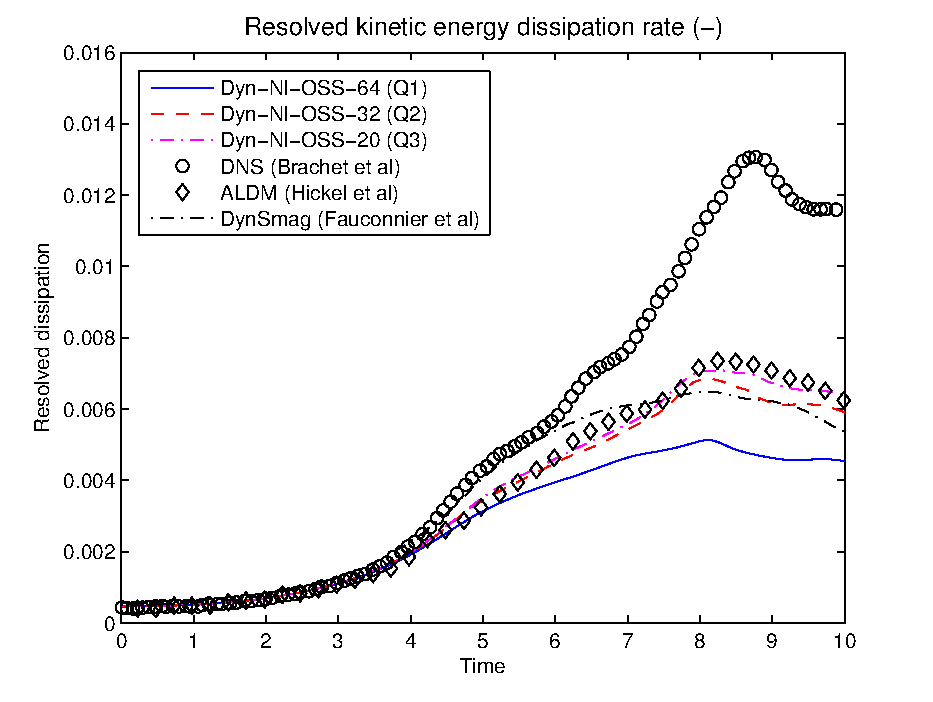
\includegraphics[width=0.49\textwidth]{Figures/TG/ens_64dofs_dynsmag_resolved}}
%	\subfigure[Total]{\label{fig:enediss_dynsmag_total}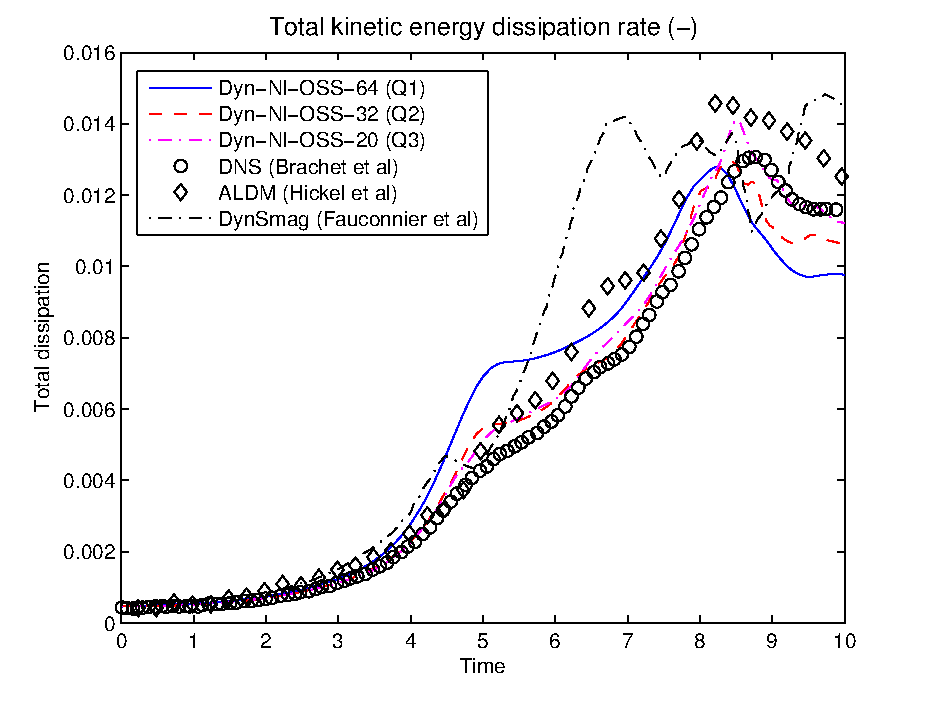
\includegraphics[width=0.49\textwidth]{Figures/TG/ens_64dofs_dynsmag_total}}
%	\caption{Dissipation rate evolution compared to the dynamic Smagorinsky \cite{fauconnier_construction_2009} and ALDM models \cite{hickel_adaptive_2006}.}
%	\label{fig:enediss_dynsmag}
%\end{figure}

It can be observed in Fig. \ref{fig:enediss_dynsmag_resolved} that all the methods produce similar results, %. , ``certainly acceptable'' according to \cite{fauconnier_construction_2009} 
The dynamic Smagorinsky is more accurate in predicting the resolved dissipation at earlier times (up to $t\approx{}6$) but less accurate at later times (see Fig. \ref{fig:enediss_dynsmag_resolved}). 
%Nevertheless, 
We plot the total dissipation in Fig. \ref{fig:enediss_dynsmag_total}. We can see that the excellent job our implicit LES model does when the $20 (Q3)$ mesh is used, which would result in an excellent prediction of the resolved kinetic energy decay (which is not available in \cite{hickel_adaptive_2006}). 

\section{Turbulent channel flow}
\label{sec-C4_TCF}
After studying the performance of VMS in the LES of homogeneous flows we turn our attention to wall-bounded turbulent flow and present results of fully developed turbulent flow in a channel.

This test consists of a fluid that flows between two parallel walls driven by an imposed pressure gradient which is defined by the Reynolds number based on the wall shear velocity, ${\rm Re}_\tau$. In the important amount of literature devoted to this problem, the usual Reynolds numbers are: ${\rm Re}_\tau=590$, ${\rm Re}_\tau=395$  and ${\rm Re}_\tau=180$ (see \cite{bazilevs_variational_2007, Calderer2013, gamnitzer_time-dependent_2010, gravemeier_algebraic_2010, gullbrand_effect_2003, hughes_large_2001, john_variants_2008, kim_turbulence_1987, masud_variational_2011, moser_direct_1999}). We will restrict our attention to ${\rm Re}_\tau=180$ and ${\rm Re}_\tau=395$. See Section \ref{sec-C3_TCF} for an extended description of this test.

\subsubsection{Setting}
\label{subsubsec-C4_TCF_setting}

We solve the problem using the coarsest mesh from previous tests, $32^3$ linear hexahedral $(Q1)$ elements. The refinement in the wall-normal direction follows a hyperbolic function, also used in \cite{Calderer2013,  gamnitzer_time-dependent_2010,  gravemeier_algebraic_2010, gullbrand_effect_2003, masud_variational_2011}, defined as 
$$y_i=\frac{\tanh\left(\gamma\left(\frac{2i}{np_y}-1\right)\right)}{\tanh(\gamma)},$$
where $i=1,...,np_y$ with $np_y$ the total amount of nodes in the wall-normal direction. Here, $\gamma$ is  chosen to be equal to $2.75$ for both  ${\rm Re}_\tau=180$ and ${\rm Re}_\tau=395$.  We refer the reader to \cite{Avila2014} for a complete study of the influence of the discretization in the results of the TCF.

As it has been said above, we solve the problem using two different friction Reynolds numbers, ${\rm Re}_\tau=180$ and ${\rm Re}_\tau=395$. We compare our results against those obtained by DNS in \cite{moser_direct_1999,kim_turbulence_1987} and we choose our parameters accordingly.
We take the bulk mean velocity and the half channel height equal to one, $\bar{U}=1$ and $\delta=1$. The viscosity is computed from the estimated Reynolds number based on the bulk mean velocity ${\rm Re}$. Then, from the friction Reynolds number ${\rm Re}_\tau$ we compute the friction velocity ($u_\tau$), the wall shear stress ($\tau_w$) and a driving force equivalent to a pressure gradient ($f_x$), given by  \cite{pope_turbulent_2000}:
$$u_\tau=\frac{\nu {\rm Re}_\tau}{\delta},\quad\quad\tau_w=\rho u_\tau^2,\quad\quad
f_x=\frac{\tau_w}{\delta}.$$

We use the Crank-Nicolson time integration scheme with a constant time step. Ham \emph{et al.}  test in \cite{ham_fully_2002} the influence of the time step for a fully implicit Finite Difference midpoint method, equivalent to Crank-Nicolson, on the statistics of a TCF DNS. They found little variation in statistical turbulence quantities up to $\delta t^+=1.6$. Following Gravemeier \emph{et al.} \cite{gravemeier_algebraic_2010}, we define a time step in wall units $\delta t^+=\frac{\delta tu_\tau^2}{\nu}\approx0.69$, which, according to \cite{ham_fully_2002}, should not affect the turbulent quantity statistics. The same authors performed 25000 time steps in order to allow the flow to develop and they collected the statistics during another 5000 time steps. A total averaging time about $500\delta/U_0$ is used in \cite{choi_effects_1994} once the statistically stable regime is achieved.

In Table~\ref{table:Channel_parameters} we present the value of the different parameters defined above for the two different friction Reynolds numbers. For the initial condition we impose a parabolic profile obtained solving the stationary Stokes problem with the driving force and viscosity defined above. Additionally, with the aim to achieve a fully developed flow earlier, we introduce a perturbation with a maximum value of $10\%$ the bulk velocity.

\begin{table}[h!]
\centering
\begin{tabular}{ccc}
\hline
${\rm Re}_\tau$&$180$&$395$\\
\hline
$\nu$&$3.5714\cdot10^{-4}$&$1.4545\cdot10^{-4}$\\
$u_\tau$&$6.4286\cdot10^{-2}$&$5.7455\cdot10^{-2}$\\
$\tau_w$&$4.1327\cdot10^{-3}$&$3.3010\cdot10^{-3}$\\
$f_x$&$4.1327\cdot10^{-3}$&$3.3010\cdot10^{-3}$\\
$\delta t$&$0.06$&$0.03$\\
\hline
\end{tabular}
\caption{Test parameters for the different friction Reynolds number.}
\label{table:Channel_parameters}
\end{table}

Our purpose is to check the VMS methods defined in Subsection \ref{subsec-C4_VMS_framework} for a wall-bounded flow. Following the computations performed for the previous tests, we solve the problem using the same cases defined in Table \ref{table:DHIT_cases} and the numerical parameters $\tau_c=0$ and $\tau_m$ are defined in the same way, now with the algorithmic constants  $c_1=12$ and $c_2=8$ (see Subsection \ref{sec-C4_effect_const}) and the characteristic length, $h$, is chosen to be the minimum element length. 
%However, in the definition of the stabilization parameters (\ref{eq-C4_tau_m})-(\ref{eq-C4_tau_c}), the characteristic length, $h$, is choosen to be the minumum element length.

\subsubsection{Velocity profiles}
We first present the mean streamwise velocity profile scaled by the wall shear stress velocity, $\langle u\rangle^+=\frac{\langle u\rangle}{u_\tau}$ for all cases defined in Table \ref{table:DHIT_cases}, where $\langle\cdot\rangle$  denotes the mean value in streamwise and spanwise direction and in time, as a function of $y^+ = \frac{y u_\tau}{\nu}$.

In Fig. \ref{fig:Channel_umean_32} we show the mean streamwise velocity normalized by the wall-shear velocity, $u_\tau$, obtained for all cases considered in Table \ref{table:DHIT_cases} in a $32^3$ linear elements mesh for the ${\rm Re}_\tau=395$ case. We compare the results with the DNS one obtained in  \cite{moser_direct_1999}. We can observe in Fig. \ref{fig:Channel_umean_32} that all methods perform quite similar and are very close to the DNS result. Fig. \ref{fig:Channel_re395_32} also depicts the streamwise, spanwise and wall-normal root mean square (rms) velocity fluctuation components normalized by the wall-shear stress velocity. 

%\begin{figure}[h!]
%	\centering	
%	\subfigure[Mean streamwise velocity]{\label{fig:Channel_umean_32}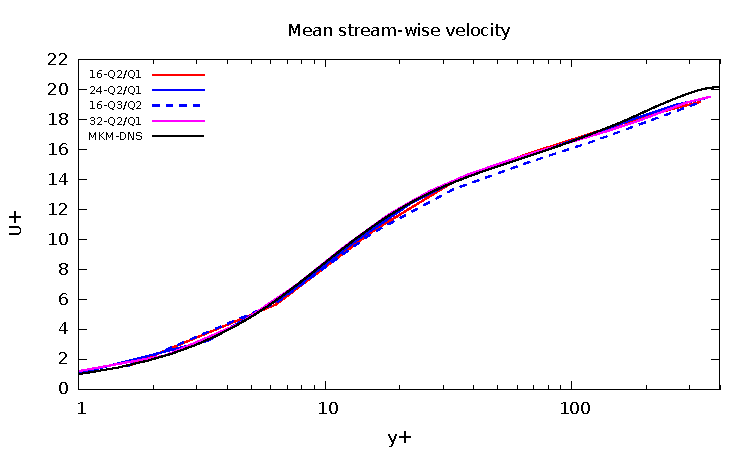
\includegraphics[width=0.49\textwidth]{Figures/CF/umean}}
%	\subfigure[Rms streamwise velocity fluctuation]{\label{fig:Channel_ufluc_32}\includegraphics[width=0.49\textwidth]{Figures/CF/ufluc}}\\   
%  	\subfigure[Rms wall-normal velocity fluctuation]{\label{fig:Channel_vfluc_32}\includegraphics[width=0.49\textwidth]{Figures/CF/vfluc}}
%  	\subfigure[Rms spanwise velocity fluctuation]{\label{fig:Channel_wfluc_32}\includegraphics[width=0.49\textwidth]{Figures/CF/wfluc}}
%	\caption{Mean streamwise velocity and rms velocity fluctuations for ${\rm Re}_\tau=395$ case using a $32^3$ $Q$1 mesh.}
%	\label{fig:Channel_re395_32}
%\end{figure}

\subsubsection{Reynolds shear stress}

Another turbulent quantity widely used in the TCF test is the Reynolds shear stress. At the continuous level the Reynolds shear stress is defined as
\begin{equation}
\label{eq-C4_Rey_shear_cont}
R_{xy}=-\left\langle u'v'\right\rangle+\nu\frac{\partial\left\langle u\right\rangle}{\partial y},
\end{equation}
being $u$ and $v$ the velocity in the streamwise direction and wall-normal direction, respectively,
and the prime denoting the fluctuations, i.e., the variable minus the mean.

It can be seen that for the discrete equation (\ref{eq-C4_NS_discrete}), one can obtain the Reynolds shear stress defined as follows:
\begin{equation}
\label{eq-C4_Rey_shear_disc}
R_{xy}=-\left\langle a_x'a_y'\right\rangle+\nu\frac{\partial\left\langle u_h\right\rangle}{\partial y}=-\underbrace{\left\langle u_h'v_h'\right\rangle}_I-\underbrace{\left\langle u_h'\tilde{v}'\right\rangle-\left\langle \tilde{u}'v_h'\right\rangle-\left\langle \tilde{u}'\tilde{v}'\right\rangle}_{II}+\underbrace{\nu\frac{\partial\left\langle u_h\right\rangle}{\partial y}}_{III}.
\end{equation}
being $a_i$ the $i$-th component of the advection velocity. In (\ref{eq-C4_Rey_shear_disc}) we have used the nonlinear definition of the advection velocity defined in (\ref{eq-C4_a_nl}).

The first term on the second part of  (\ref{eq-C4_Rey_shear_disc}) (term $I$) is the contribution of the resolved scales (FE component) to the cross term $\left\langle a_x'a_y'\right\rangle$. Term $II$ denotes the contribution of the subgrid scales and their interaction with the FE components, that is, the unresolved part of the equation. Finally, term $III$ accounts for the viscous portion of the Reynolds shear stress. Note that the derivatives of the approximated subscales are not computable, since these approximated subscales are discontinuous and have been designed to approximate the effect of the exact subscales on the FE scales elementwise. 

For a fully developed and statistically stable turbulent flow, the Reynolds shear stress along the wall-normal direction has a linear shape  (see \cite{kim_turbulence_1987}). Normalized by the viscous term $III$ value at the wall, the total Reynolds shear stress in terms of $y/	\delta$ should have the following expression: $R_{xy}(y/\delta)=(-y/\delta)$. Fig.~\ref{fig:OSS_dyn_Nl_reystr} depicts the absolute value of the Reynolds shear stress along the upper half channel ($y>0$), with the different terms appearing in (\ref{eq-C4_Rey_shear_disc}) and compared with the DNS in \cite{moser_direct_1999}, for the Dyn-Nl-OSS case with ${\rm Re}_\tau=395$. The computed results are almost identical to the DNS ones. It has to be noted that the computed results are evaluated at the integration points due to the presence of the derivative in the Reynolds shear stress, which using linear FEs is constant at each element. Then, using two integration points per direction for the numerical integration, term $III$ will be constant for those two integration points being in the same element. This behavior is observed in Fig.~\ref{fig:OSS_dyn_Nl_reystr}, where the viscous term is pairwise constant. This last fact also affects the total Reynolds shear stress. Since the resolved term has different values at each element Gauss point, the sum of terms $I$ and $III$ results in an oscillatory shape near the wall, where the viscous term is more relevant. It is also seen that the unresolved term $II$ does not contribute to the Reynolds shear stress, which is a good property of the tested VMS methods. The results for the remaining cases in Table \ref{table:DHIT_cases} are similar to those presented in Fig. \ref{fig:OSS_dyn_Nl_reystr} and have not been reported. 
%\begin{figure}[h!]
%	\centering	
%	\includegraphics[width=0.5\textwidth]{Figures/CF/reystr_395_Dyn_Nl_OSS}
%	\caption{Reynolds stress of the Dyn-Nl-OSS case.}
%	\label{fig:OSS_dyn_Nl_reystr}
%\end{figure}
%% SB: Some change?
%%{\color{blue} Esta seccion está perfecta, no tengo que tocar nada. However, si en la turbulencia homogenea calculamos los resultados usando $\u_h$ solamente...porque aca incluimos tambien $\tilde{\u}$?}

\section{Sensitivity with respect to the stabilization parameters}
\label{sec-C4_effect_const}

All the VMS models considered herein depend on the stabilization parameters $\tau_m$ and $\tau_c$, which contain constants $c_1$ and $c_2$ whose value is chosen from numerical experiments. However, we can infer from (\ref{eq-C4_static_energy}) or (\ref{eq-C4_transfer}) how this dependency will be. As mentioned before, the last two terms in (\ref{eq-C4_transfer}) are dissipative and therefore, increasing $\tau_m$ and/or $\tau_c$ we obtain a more dissipative method. From (\ref{eq-C4_tau_m})-(\ref{eq-C4_tau_c}), increasing $\tau_m$ results in a reduction of $\tau_c$. More precisely 
\begin{equation}
\label{eq-C4_tau_c_new}
\tau_c=\nu + \frac{c_2}{c_1}{|\a|}{h}
\end{equation}
from where we see that increasing $c_1$ reduces both $\tau_m$ and $\tau_c$ but increasing $c_2$ reduces $\tau_m$ but increases $\tau_c$. On the other hand, only the fourth term in (\ref{eq-C4_transfer}) is essential to control
$ \tau_{m} \left\| \mathcal{P} \left( \mathbf{a}\cdot \mathbf{\nabla u}_{h}+\mathbf{\nabla }p_{h}\right) \right\|^{2} $ and it is possible to choose $\tau_c=0$. 

The results presented above have been obtained using different settings of the numerical stabilization parameters $\tau_m$ and $\tau_c$. In DHIT and TGV tests, we take the algorithmic constants $c_1=12$ and $c_2=2$ for $\tau_m$ and we set $\tau_c=0$, while for the TCF test we have used $c_1=12$ and $c_2=8$ for $\tau_m$ and also $\tau_c=0$. In this section we analyze the influence of these parameters on the numerical results and justify our choice of the constants for the large eddy simulation of turbulent flows.

We have performed a sensitivity analysis of the VMS schemes with respect to the value of $c_1$ and $c_2$. To see the effect of such algorithmic constants on $\tau_m$ and $\tau_c$ independently, we define a new constant $c_c$ which allows us to redefine (\ref{eq-C4_tau_c_new}) as
\begin{equation}
\label{eq-C4_tau_c_cc_new}
\tau_c=c_c\left(\nu + \frac{c_2}{c_1}{|\a|}{h}\right)
\end{equation}
These experiments have been done for the DHIT test using the Dyn-Nl-OSS case in a $32^3$ $Q$1 mesh and the results are depicted in Fig.~\ref{fig:tau_analysis}. They show important changes in the dissipation the VMS methods introduce when constants are changed. %, as energy dissipation and energy spectra. 
%{\color{blue} 
It is known that the decay rate of kinetic energy in isotropic turbulence is driven by large scales (of the order of the integral scale) (see, e.g., \cite{comte-bellot_simple_1971}). As we have observed, the subgrid model has only influence when a very coarse grid is used.
%} 

In particular, for high Reynolds number problems, the constant $c_1$ does not have so much influence on $\tau_m$, but it does on $\tau_c$. With respect to $c_2$, we observe that it influences the energy dissipation of the method, which is increased when the value of this constant is decreased. When $\tau_c$ is activated ($c_c=1)$, we observe a growth of the energy dissipation when the coefficient $c_2/c_1$ increases. This behavior is what we are expecting since the method becomes more diffusive  when $\tau_c$ is increased due to the last term in (\ref{eq-C4_transfer}).


Concerning the energy spectra, it is also shown in Fig.~\ref{fig:spec_tauc0_t04} and Fig.~\ref{fig:spec_tauc0_t08} that the only constant that influences the result when $\tau_c=0$ is $c_2$. In these figures we can see that when we increase $c_2$ the method is less dissipative, resulting in an inappropriate slope of the energy spectra. We can observe that with $c_2=2$ the decay of the energy behaves correctly, keeping the $k^{-5/3}$ law. For the largest values of $c_2$ the energy at small scales is not properly dissipated. Note that for $c_2=2$ the slope of the energy spectrum is kept almost constant along the time, which does not happen in the other cases. When we activate $\tau_c$ (see Figs. \ref{fig:spec_tauc1_t04} and \ref{fig:spec_tauc1_t08}) we are introducing additional dissipation into the system that eliminates the pile up of the energy spectra for all the cases, but generally results in steeper slopes. Here we also have to note that the energy spectra slope is time dependent for all cases except for $c_2=2$.
%{\color{red} To improve with references and better explanation of the energy spectra correct behavior}
This analysis led us to choose $c_1=12$ and $c_2=2$ for $\tau_m$ and set $\tau_c=0$ for homogeneous turbulence, i.e., DHIT and TGV tests.

%%\begin{figure}[h!]
%%  \centering
%%  \subfigure[Energy with $c_1=12$, $c_2=8$ and $c_c$ variable]{\label{fig:tau_analysis_cc} 
%%  \includegraphics[width=0.49\textwidth]{Figures/DHIT/ene_tauc_close}}    
%%  \subfigure[Energy with $c_1$ and $c_2$ variable and $c_c=0$]{\label{fig:tau_analysis_c12}
%%  \includegraphics[width=0.49\textwidth]{Figures/DHIT/ene_taum_close}}
%%  \caption{Comparison of the global energy in the DHIT test for Dyn-Nl-OSS method using a $32^3$ $Q$1 mesh}
%%  \label{fig:tau_analysis}
%%\end{figure}
%
%% \afterpage{
%% \begin{landscape}
%\begin{figure}[h!]
%\begin{center}
%%\begin{tabular}{c@{}c@{}c@{}c}
%\begin{tabular}{@{}c@{}c}
%%\multirow{2}{*}{\subfigure[Legend]{\label{fig:legend}
%%\includegraphics[clip=true,trim=14cm 15cm 16cm 4cm,width=0.2\textwidth]{Figures/DHIT/legend}}} &
%%\subfigure[Global energy with $c_c=0$]{\label{fig:ene_tauc0}
%%\includegraphics[width=0.42\textwidth]{Figures/DHIT/ene_tauc0}} &
%\subfigure[Energy spectra at $t=0.4$ with $c_c=0$]{\label{fig:spec_tauc0_t04}
%\includegraphics[width=0.48\textwidth]{Figures/DHIT/spec_tauc0_t04}} &
%\subfigure[Energy spectra at $t=0.8$ with $c_c=0$]{\label{fig:spec_tauc0_t08}
%\includegraphics[width=0.48\textwidth]{Figures/DHIT/spec_tauc0_t08}} \\
%%\subfigure[Global energy with $c_c=1$]{\label{fig:ene_tauc1}
%%\includegraphics[width=0.42\textwidth]{Figures/DHIT/ene_tauc1}} &
%\subfigure[Energy spectra at $t=0.4$ with $c_c=1$]{\label{fig:spec_tauc1_t04}
%\includegraphics[width=0.48\textwidth]{Figures/DHIT/spec_tauc1_t04}} &
%\subfigure[Energy spectra at $t=0.8$ with $c_c=1$]{\label{fig:spec_tauc1_t08}
%\includegraphics[width=0.48\textwidth]{Figures/DHIT/spec_tauc1_t08}} \\
%\multicolumn{2}{c}{\subfigure[Legend]{\label{fig:legend}
%\includegraphics[clip=true,trim=0cm 0cm 0cm 0cm,width=0.6\textwidth]{Figures/DHIT/legend2}}}
%\end{tabular}
%\end{center}
%\caption{Comparison of energy spectra for different $c_1$, $c_2$ and $c_c$ in the DHIT test.}
%\label{fig:tau_analysis}
%\end{figure}
%%\end{landscape}
%%}
%
%%{\color{blue}Looking at Figure \ref{fig:tau_analysis}, it seems that the decision to choose $c_1=12$ and $c_2=2$ for $\tau_m$ and set $\tau_c=0$ is the best option among those analysed} {\color{red} for homogeneous turbulence, i.e., DHIT and TGV tests????}.
%
%%{\color{blue}
In order to go in depth on the effect of the algorithmic constants $c_1$ and $c_2$ and the stabilization parameter $\tau_c$ of the incompressibility equation, we compare the results for the TCF problem with a friction Reynolds number ${\rm Re}_\tau=180$ using the same choice made for homogeneous turbulence 
%the setting used until now 
($c_1=12$, $c_2=2$ and $\tau_c=0$) against the setting of the incompressible case in \cite{Avila2014} ($c_1=12$, $c_2=2$ and $\tau_c$ as in (\ref{eq-C4_tau_c})) and a less dissipative setting with $c_1=12$, $c_2=8$ and $\tau_c=0$. These tests have been done using the Dyn-Nl-OSS case in a $32^3$ $Q1$ mesh.

%\begin{figure}[h!]
%	\centering	
%	\subfigure[Mean streamwise velocity]{\label{fig:OSS_taus_umean}\includegraphics[width=0.49\textwidth]{Figures/CF/umean_taus_DOSS}}
%  	\subfigure[Rms streamwise velocity fluctuation]{\label{fig:OSS_Matias_ufluc}\includegraphics[width=0.49\textwidth]{Figures/CF/ufluc_taus_DOSS}}\\    
%  	\subfigure[Rms wall-normal velocity fluctuation]{\label{fig:OSS_Matias_vfluc}\includegraphics[width=0.49\textwidth]{Figures/CF/vfluc_taus_DOSS}}
% 	\subfigure[Rms spanwise velocity fluctuation]{\label{fig:OSS_Matias_wfluc}\includegraphics[width=0.49\textwidth]{Figures/CF/wfluc_taus_DOSS}}
% 	\caption{Comparison of mean streamwise velocity and rms velocity fluctuations for ${\rm Re}_\tau=180$ case using a $32^3$ $Q$1 mesh.}
%    \label{fig:OSS_taus_fluc}
%\end{figure}

In Fig. \ref{fig:OSS_taus_umean} the mean velocity in the streamwise direction is shown. As in the case of homogeneous turbulence, some differences between the three cases can be observed, the choice used in section \ref{sec-C4_TCF} being the most accurate one. The effect of the algorithmic constant $c_2$ and the stabilization parameter $\tau_c$ in the problem solution can be clearly observed, i.e., the less dissipative choice gives the best results.
%Not only  $\tau_c=0$ but also setting $c_2=8$ (instead of $c_2=2$) give less dissipative results.
Figs. \ref{fig:OSS_Matias_ufluc}, \ref{fig:OSS_Matias_vfluc} and \ref{fig:OSS_Matias_wfluc} depict the rms velocity fluctuations in all directions. The fluctuations in the streamwise direction are better predicted using ($c_1=12$, $c_2=8$ and $\tau_c=0$) but the spanwise and wall-normal directions are not.

\section{Behavior in the small time step limit}
\label{sec-C4_small_time_step}

Small time step instabilities for VMS LES simulations of turbulent flows have been reported in \cite{Hsu2010,gamnitzer_time-dependent_2010}. In these references, the VMS models differ from the ones in this work. Instead of the definition of  $\tau_m$ in (\ref{eq-C4_tau_m}), a time step dependent stabilization parameter $\tau_m$
$$
\tau_m=\left(\frac{1}{\delta t} + \frac{c_1\nu}{h^2}+\frac{c_2|\a|}{h}\right)^{-1},\\
$$
is considered in all cases.\footnote{The parameter $\tau_{m,t}$ for the dynamic subscales model also
scales with $\delta t$, as discussed in Section (\ref{sec-C4_discrete}). {\it However}, this dependence comes from a consistent time integration of the subscale time derivative (see also \cite[Section 3.2]{codina_time_2007}).} The plain introduction of a time step dependency in $\tau_m$ faces serious difficulties:
\begin{itemize}
\item The method becomes unstable in the small time step limit since it converges to the unstable Galerkin formulation.
%\item A similar situation occurs in the Navier-Stokes problem if $\tau_c=0$.
\item If $\tau_c$ is computed from (\ref{eq-C4_tau_c}) (as it is usually done, see, e.g., \cite{bazilevs_variational_2007,Hsu2010,gamnitzer_time-dependent_2010,gravemeier_algebraic_2010}), $\tau_m \sim \delta t$ and $\tau_c \sim \delta t^{-1}$ in the small time step limit. If this approach is followed , the essential numerical dissipation given by the fifth term in (\ref{eq-C4_static_energy}) is reduced as $\delta t \to 0$, whereas the numerical dissipation introduced by the last term in the left hand side (a incompressibility penalty term) of (\ref{eq-C4_static_energy}) is increased. It has a compensating effect in practice, but the penalty term does not properly act as a turbulence model. % , as shown in the previous section.
\end{itemize}
%The behavior of the VMS models considered herein in the small time step limit is evaluated numerically in Section \ref{sec-C4_TCF}.

Let us perform a test to study the small time step behavior of the VMS methods presented in Section \ref{sec-C4_formulation}, using the skew-symmetric \textit{type 1} form of the convective term, as in previous numerical experiments. We also include a combination we do not advocate here, static subscales and nonlinear splitting, an approach followed in \cite{Calo_2004,bazilevs_variational_2007,Hsu2010,gamnitzer_time-dependent_2010,gravemeier_algebraic_2010}. %The properties of the different methods in this respect have been discussed in Section \ref{sec-C4_small_time_step}. 
The behavior of all the methods for the TCF test with $\delta t=0.002$ is summarized in Table \ref{table:small_time_step_T}, where YES means that the simulation was successful, NO means that the simulation diverged and $\delta t\downarrow$ means that the simulation was successful only when the adaptive time step strategy described in Section \ref{subsubsec-C4_DHIT_setting} was used.

%It is worth to point out that all these results have been obtained using the skew-symmetric \textit{type 1} form of the convective term, which exactly conserves energy. %Either a conservative or non conservative form is usually employed mentioned references and none of this forms conserve energy. As we have shown in Section \ref{subsubsec-C4_ene_cons_DHIT} for the skew-symmetric \textit{type 2}, they could be productive. 
It is important to note that the static and nonlinear ASGS formulation used in \cite{bazilevs_variational_2007,Hsu2010,gamnitzer_time-dependent_2010,gravemeier_algebraic_2010} with the convective term \textit{type 2} becomes unstable after some time, as also reported in these works, even for the time step size defined in section \ref{subsubsec-C4_TCF_setting}. However, using the the skew-symmetric \textit{type 1} form of the convective term, which exactly conserves energy, the simulation ended successfully for the time step defined in section \ref{subsubsec-C4_TCF_setting}, but failed to converge with the small one. This result is a numerical evidence of the fact that the use of convective terms without the skew-symmetric property produce energy (see also Section \ref{subsubsec-C4_Total_ene_DHIT}) that can make simulations unstable. Further, \emph{these results evidence once again that it is a good choice to stick to provably unconditionally stable formulations, i.e., the dynamic formulations and/or orthogonal subscales formulations with a skew-symmetric convective term}. %{\color{blue} 
Similar results have been reported in the finite difference context in \cite{verstappen_symmetry-preserving_2003}, where it is shown that stable simulations of the TCF can be performed using an energy-preserving skew-symmetric formulation.
%}

\begin{table}[h!]
%\label{tab:small_dt}
%\footnotesize
\centering
\begin{tabular}{ccccccccc}
\hline
Method&\multicolumn{4}{c}{ASGS}&\multicolumn{4}{c}{OSS}\\\hline
Tracking&\multicolumn{2}{c}{Static}&\multicolumn{2}{c}{Dynamic}&\multicolumn{2}{c}{Static}&\multicolumn{2}{c}{Dynamic}\\\hline
Advection&Linear&Nonlinear&Linear&Nonlinear&Linear&Nonlinear&Linear&Nonlinear\\\hline
Converged&Yes&No&Yes&Yes&$\delta t\downarrow$&$\delta t\downarrow$&Yes&Yes\\\hline
\end{tabular}
\caption{Small time step convergence analysis.}
\label{table:small_time_step_T}
\end{table}

%Furthermore, keeping aside the stability of the methods, 
To the best of our knowledge, the stability (or instability) of dynamic ASGS methods has not been proved. In our numerical experiments the static and dynamic linear versions fail to converge in some problems (e.g DHIT) but we have not found these problems with the Dyn-Nl-ASGS method. Nevertheless, we have found an important increase in the computational cost when the time step is reduced. 
%the time step size also has an effect on the computational cost. 
%In particular, the number of solver iterations for ASGS methods increase when the time step is reduced. 
This behavior is explained in Fig. \ref{fig:1st_step_comp_cost}, where the number of solver iterations at the first time step is plotted against the time step size for the dynamic and nonlinear cases of ASGS and OSS methods, with $32^3$ and $64^3$ $Q1$ mesh, for the DHIT test case. \emph{The number of required solver iterations (and as a result the condition number of the system matrix) blows up exponentially for the ASGS method as we reduce the time step size, whereas it remains constant for the OSS method.} This important observation explains the computational cost trends observed in the previous section.

%\begin{figure}[h!]
%	\centering	
%	\includegraphics[width=0.5\textwidth]{Figures/DHIT/1st_step_comp_cost}
%	\caption{Solver iterations at the first time step for DHIT test.}
%	\label{fig:1st_step_comp_cost}
%\end{figure}

%Finally, it is clearly seen in Fig. \ref{fig:1st_step_comp_cost} the exponential increase of solver iterations for the ASGS methods when the time step tends to zero, independently of the mesh size. This performance denotes the \emph{ill conditioning of the ASGS system matrix with respecto to the time step size}. On the other hand, \emph{the number of solver iterations remains constant for the OSS method}, regardless of the time step size.

%%\subsubsection{Numerical dissipation}
%%
%%\begin{figure}[h!]
%%	\centering	
%%	\includegraphics[width=0.5\textwidth]{Figures/CF/numdis_395_Dyn_Nl_OSS}
%%	\caption{Numerical dissipation of the Dyn-Nl-OSS case}
%%	\label{fig:OSS_dyn_Nl_numdis}
%%\end{figure}
%
\section{Conclusions}
\label{sec-C4_conclusions}

In this paper we have assessed the performance of the numerical formulations previously developed in our group \cite{codina_stabilized_2002,codina_time_2007,Codina-chap-2011,Principe2009} for turbulent incompressible flow problems. 

The methods proposed are different to those whose testing in turbulent regimes has been published before, the closest ones being those reported in \cite{bazilevs_variational_2007,gamnitzer_time-dependent_2010}. First, we consider orthogonal subscales formulations. Further, in \cite{bazilevs_variational_2007} the ASGS method with quasi-static subscales is used (in the isogeometrical analysis context) but the time step dependency is included in the stabilization parameter (with the inconsistencies and problems discussed in section \ref{sec-C4_small_time_step}) and the nonlinear scale splitting is applied in the FE equation only (not in the subscale equation). Time dependent subscales are used in \cite{gamnitzer_time-dependent_2010}, but the authors consider a linear scale splitting. Furthermore, in both works $\tau_c \neq 0$. 

First, we have discussed some theoretical aspects, such as the dissipative structure of the methods and the way energy is conserved, which we have numerically verified. Related to this point, we analyze the effect of using different skew-symmetric forms of the convective term, and its impact on energy conservation; if a skew symmetric form is not used, negative energy dissipation can be introduced to the scheme, which may be a source of instability. 

However, the most important conclusions come from the different problems that we have solved numerically. Overall, OSS and ASGS yield similar results, all displaying the features of turbulent flows, reproducing appropriately global outputs such as energy spectra. The methods are stable and converge to reference solutions, both when the mesh is refined and when the polynomial order is increased. 

On the other hand, we have thoroughly analyzed the effect of the algorithmic constants for isotropic turbulence and wall-bounded turbulent flows, and chosen them based on this sensitivity analysis. An important observation in this line is the fact that all the methods considered in this work are certainly sensitive to the algorithmic constants and they have to be properly chosen in order to simulate turbulent flows on coarse meshes. In fact, the differences in the numerical results are much more influenced by the algorithmic constants than by the choice of the VMS formulation itself.  This strong influence seems to be a characteristic feature of turbulence, since in our experience it is not so important in laminar flows. VMS methods is something that needs further research.

Further, we have analyzed the effect of small time steps when the stabilization parameters depend on them.


Apart from the quality of the results, the OSS method with dynamic subscales is convenient in terms of numerical performance. It requires more nonlinear iterations than ASGS, but less iterations of the linear solver, altogether leading to lower computational cost. In both formulations, ASGS and OSS, the use of dynamic subscales has been found to be crucial for nonlinear convergence. In fact, in some cases quasi-static subscales failed to converge. We have explained these facts by plotting the number of solver iterations required to converge as we reduce the time step size, for a fixed mesh in space. The number of iterations (and as a result the condition number of the system matrix) blows up exponentially for ASGS whereas it remains bounded for OSS.
\chapter{Term-by-term Orthogonal Subscales with inf-sup stable elements}
\label{chap-TBT_OSS}

\section{Introduction}
\label{sec-C5_intro}

The VMS method for incompressible turbulent flows has been analysed previously in Chapter \ref{chap-Rb_VMS}. As stated there, the VMS method introduced by Hughes in \cite{hughes_multiscale_1995,hughes_variational_1998} is a framework to develop stable and accurate numerical approximations of partial differential equations, preventing numerical instabilities that arise when the standard Galerkin FE method is used. 

We also recall here that the use of VMS method as an ILES method was firstly suggested in \cite{hughes_multiscale_2001,hughes_large_2001,codina_stabilized_2002} and, since then, several VMS methods have been developed and used as ILES. We can distinguish between those that introduce a three scale decomposition into resolved large and small scales and unresolved scales \cite{koobus_variational_2004,john_variants_2008, john_numerical_2010, masud_variational_2011}, with a Smagorinsky type model for the influence of unresolved scales onto the small resolved ones, and those that introduce a two scale decomposition into resolved and unresolved ones \cite{bazilevs_variational_2007,colomes_assessment_2015} using a residual based or projection based model of the unresolved scales to account for their influence into the resolved ones.

In \cite{codina_stabilization_2000}, a two scale VMS approach through OSS was firstly introduced. The main idea of the OSS method is to select the space of small scales orthogonal to the FE space, in contrast to the traditional choice of taking the subscales proportional to the residual, which is called ASGS in \cite{codina_stabilization_2000}. Apart from the choice of the space of subscales, their time dependency and the VMS splitting of nonlinear terms was studied in \cite{codina_time_2007}. Several combinations of these modelling possibilities where exhaustively assessed for homogeneous and wall bounded turbulent flows in \cite{colomes_assessment_2015}\footnote{Chapter \ref{chap-Rb_VMS} collects most of the work exposed in \cite{colomes_assessment_2015}, which has been extended and adapted to fit in the argumentation of this thesis.}. In that work, an explicit algorithm to compute the orthogonal projections was used and the projection of the whole residual was considered.

An alternative definition of the OSS method was proposed in \cite{codina_analysis_2008} using a term-by-term stabilization that does not involve the full residual. A similar term-by-term stabilization approach was followed in \cite{braack_local_2006}, where the Local Projection Stabilization (LPS) method was introduced. This type of techniques are also known as symmetric projection stabilization, and the key ingredient that leads to different schemes is the definition of such projection \cite{braack_local_2006,badia_stabilized_2012}. One of the main interests of a term-by-term stabilization is that one can avoid the addition of the pressure gradient stabilization term when using \textit{inf-sup} stable (ISS) velocity-pressure pairs. Another advantage of the \textit{term-by-term} stabilization methods is that the projection can be easily treated as implicit, without having all the residual terms coupled. The use of equal-order or ISS pairs with the LPS method was assessed for laminar flows in \cite{g_lube_local_2008}, concluding that the grad-div stabilization term is more relevant than the convective stabilization term when ISS FEs are used. The same conclusion was pointed out in \cite{john_numerical_2010}, where the turbulent channel flow is studied using a projection-based and a bubble-based FE VMS method introducing a Smagorinsky type model to stabilize convection. 

The main goal of this chapter is to assess for the first time the accuracy and efficiency of convection-stabilized ISS schemes as ILES methods, where symmetric projection stabilization is used. In particular, we analyze the term-by-term OSS method with implicit treatment of the projection for turbulent flows. We also analyse the influence of the grad-div stabilization on the accuracy of the method. For ISS discretizations, the influence of this term on the mass conservation is well known \cite{linke_collision_2009} but it also influences the computational cost of the linear solvers \cite{olshanskii_grad-div_2004,heister_efficient_2013}. In this respect, we present a block preconditioning strategy that makes use of recursive block factorizations \cite{badia_block_2014} to deal with the implicit projections and with the saddle point structure of the velocity-pressure coupling, which can also be applied to equal order interpolation with pressure stabilization. The comparison of the results is made with respect those obtained using the residual-based ASGS for which we also use a block preconditioning strategy.

This chapter is organized as follows. The Navier-Stokes equations together with some notation used in the paper are stated in Section~\ref{sec-C5_prob_statment}. The VMS framework is introduced in Section~\ref{sec-C5_VMS_framework}, which includes the final discrete formulation of the ASGS method, given in Section~\ref{subsec-C5_ASGS}, the term-by-term OSS given in Section~\ref{subsec-C5_OSStbt}, the term-by-term OSS with ISS elements given in Section~\ref{subsec-C5_OSSiss} and also a brief discussion of known properties of the grad-div stabilization given in Section~\ref{subsec-C5_pressure_subscale}. The recursive block iterative strategy proposed to solve the linear system of the monolithic problem is presented in Section~\ref{subsec-C5_block_precond}. The numerical results are shown in Section~\ref{sec-C5_results}, where two different turbulent tests are analysed: the Taylor-Green Vortex flow in Section \ref{subsec-C5_TGV-VMS} and the Turbulent Channel Flow in Section \ref{subsec-C5_turb_channel}. Finally, some conclusions are pointed out in Section \ref{sec-conclusions}.

\section{Problem statement}
\label{sec-C5_prob_statment}
For the sake of chapter completness, let us retrieve the problem definition described in chapter \ref{chap-Perliminaries}, albeit rather briefly.

Let $\Omega$ be a bounded domain of $\mathbb{R}^d$, where $d=2,3$ is the number of space dimensions, $\Gamma=\partial\Omega$ its boundary and $(0,T]$ the time interval. The strong form of the steady Navier-Stokes problem consists in finding the velocity field $\u$ and the pressure field $p$ such that 
\begin{align}
\label{eq-C5_NS_strong_mome}
\partial_t\u-\nu\Delta\u+\u\cdot\nabla\u+\nabla p&=\f&\mbox{in $\Omega\times(0,T]$,}\\
\label{eq-C5_NS_strong_inc}
\nabla\cdot\u&=0&\mbox{in $\Omega\times(0,T]$,}
\end{align}
with $\f$ the force vector and $\nu$ the kinematic viscosity. Equations \Eq{C5_NS_strong_mome} and \Eq{C5_NS_strong_inc} need to be supplied with appropriate boundary and initial conditions. The boundary $\Gamma$ is divided into the Dirichlet ($\Gamma_D$) and the Neumann ($\Gamma_N$) parts such that $\Gamma_D\cup\Gamma_N=\Gamma$ and $\Gamma_D\cap\Gamma_N=\O$. Then, the boundary and initial conditions can be written as
\begin{align}
\label{eq-C5_NS_strong_Dir}
\u&=\u_g&\mbox{on $\Gamma_D\times(0,T]$,}\\
\label{eq-C5_NS_strong_Neu}
(-p\cdot\mathbf{I}+\nu(\nabla\u+\nabla\u^T))\cdot\mathbf{n}&=\mathbf{t}_N&\mbox{on $\Gamma_N\times(0,T]$,}\\
\label{eq-C5_NS_strong_Ini}
\u(\x,0)&=\u_0(\x)&\mbox{in $\Omega\times\{0\}$,}
\end{align}
$\mathbf{n}$ being the unit outward vector normal to $\Gamma$.

From equations \Eq{C5_NS_strong_mome}-\Eq{C5_NS_strong_Ini} one can derive the weak form of the problem, which consists in finding $[\u,p]\in\mathbf{L}^2(0,T;\mathcal{V}_g)\times L^1(0,T;\mathcal{Q}_0)$ such that
\begin{equation}
\label{eq-C5_NS_weak}
(\partial_t\u,\v)+B(\u,(\u,p),(\v,q)) = \left<\f,\v\right> 
\quad\quad\forall\v\in\mathcal{V}_0,\quad\forall q\in\mathcal{Q}_0,
\end{equation}
satisfying the initial condition \Eq{C5_NS_strong_Ini} in a weak sense. Here $\mathcal{V}_0:=\mathbf{H}_0^1(\Omega)$, $\mathcal{V}_g:=\mathbf{H}_g^1(\Omega)$  and $\mathcal{Q}_0:=L^2(\Omega)/\mathbb{R}$ and the form $B(\u,(\u,p),(\v,q))$ is defined as 
\begin{equation}
\label{eq-C5_bilinear}
B(\u,(\u,p),(\v,q)):=\nu(\nabla\u,\nabla\v)+b(\u,\u,\v)-(p,\nabla\cdot\v)+(q,\nabla\cdot\u)
\end{equation}
with the trilinear form of the convective term $b(\u,\v,\w)$ defined in its skew symmetric version
\begin{equation}
\label{eq-C5_conv_skew}
b(\u,\v,\w)=\frac{1}{2}(\u\cdot\nabla\v,\w)-\frac{1}{2}(\v,\u\cdot\nabla\w)+\frac{1}{2}(\v,(\u\cdot\mathbf{n})\w)_{\Gamma_N}.
\end{equation}

\section{VMS framework}
\label{sec-C5_VMS_framework}

Let us consider a FE partition $\mathcal{T}_h$ of the domain $\Omega$ from which we can construct conforming finite dimensional spaces for the velocity $\mathcal{V}_{0,h} \subset \mathcal{V}_0$, $\mathcal{V}_{g,h} \subset \mathcal{V}_g$, and for the pressure $\mathcal{Q}_{0,h}\subset \mathcal{Q}_0$. The Galerkin FE approximation of the problem \Eq{C5_NS_weak} consists in 
finding $[\u_h,p_h]\in\mathbf{L}^2(0,T;\mathcal{V}_{g,h})\times L^1(0,T;\mathcal{Q}_{0,h})$ such that
\begin{equation}
\label{eq-C5_NS_galerkin}
(\partial_t\u_h,\v_h)+B(\u_h,(\u_h,p_h),(\v_h,q_h)) =\left<\f,\v_h\right>
\quad\quad\forall\v_h\in\mathcal{V}_{0,h},\forall q_h\in\mathcal{Q}_{0,h}.
\end{equation}
In order to overcome the numerical instabilities and, eventually, to bypass the \textit{inf-sup} condition that arises when problem \Eq{C5_NS_galerkin} is solved, we use the VMS approach \cite{hughes_multiscale_1995,hughes_variational_1998} which consists in a two-scale decomposition of spaces $\mathcal{V}_0$, $\mathcal{V}_g$ and $\mathcal{Q}_0$ as $\mathcal{V}_0=\mathcal{V}_{0,h}\oplus\widetilde{\mathcal{V}}_0$, $\mathcal{V}_g=\mathcal{V}_{g,h}\oplus\widetilde{\mathcal{V}}_g$ and $\mathcal{Q}=\mathcal{Q}_{0,h}\oplus\widetilde{\mathcal{Q}}_0$, where $\widetilde{\mathcal{V}}_0$, $\widetilde{\mathcal{V}}_g$ and $\widetilde{\mathcal{Q}}_0$ are infinite-dimensional spaces that complete the FE spaces in $\mathcal{V}_0$, $\mathcal{V}_g$ and $\mathcal{Q}_0$, respectively. Hereinafter the subscript $(\cdot)_h$ will denote the FE component and the tilde $\widetilde{(\cdot)}$ the subgrid component. Applying the two-scale decomposition to (\ref{eq-C5_NS_weak}) we obtain
\begin{equation}
\label{eq-C5_NS_vms}
(\partial_t\u_h,\v_h)+(\partial_t\tilde{\u},\v_h)+B(\u;[\u_h,p_h],[\v_h,q_h])-\left(\tilde{\u},\nu\Delta\v_h+\a\cdot\nabla\v_h+\nabla q_h\right)_h-\left(\tilde{p},\nabla\cdot\v_h\right)=\left<\f,\v_h\right>,
\end{equation}
where $(\cdot,\cdot)_h=\sum_{K\in\mathcal{T}_h}(\cdot,\cdot)_K$ is the sum of scalar products \Eq{C5_scalar_product} over each element $K$ of the partition $\mathcal{T}_h$.
The terms involving the subscales come from an element-wise integration by parts, in which the boundary terms 
$\left( \v_{h},\nu \n\cdot \nabla \tilde{\u}\right)_{\partial h}$ and
$\left( q_{h},\n\cdot \tilde{\u}\right)_{\partial h}$
have been neglected (the subscript ${\partial h}$ is used to denote the sum over all elements of the integral on the boundary of each element). It also involves the approximation 
$b(\a,\tilde{\u},\u_h) \approx -(\tilde{\u},\a\cdot\nabla\v_h)$
which implies neglecting 
$\left( \v_{h},\n\cdot \a \tilde{\u}\right)_{\partial h}$ and
$(\tilde{\u},\nabla\cdot\a \, \v_h)$. 
These approximations are discussed in  \cite{codina_time_2007} together with the choice of $\a$ which defines the type of scale splitting (linear or nonlinear), see also \cite{colomes_assessment_2015}.

Problem \Eq{C5_NS_vms} depends on $\tilde{\u} \in \widetilde{\mathcal{V}}_0$ and on $\tilde{p}\in \widetilde{\mathcal{Q}}_0$,  $\widetilde{\mathcal{V}}_0$ and $\widetilde{\mathcal{Q}}_0$ being infinite-dimensional. Therefore, the equations for $\tilde{\u}$ and $\tilde{p}$ obtained after applying the two-scale decomposition cannot be directly solved, but some modelling steps are needed to obtain a feasible method. In this work we consider the velocity subscale as linear ($\a=\u_h$) and quasi-static, while the pressure subscale is neglected when equal order interpolation is used. Different approaches could be used for the definition of the subscales, see Chapter \ref{chap-Rb_VMS} for a deep explanation of the different choices and their numerical evaluation with equal order approximation. After the approximation of the  Navier-Stokes operators by the stabilization parameters $\tau_m^{-1}$  and $\tau_c^{-1}$ (see for example \cite{codina_time_2007}), and introducing the fine scales definitions into \Eq{C5_NS_vms} we get the final discrete problem
\begin{equation}
\label{eq-C5_NS_discrete}
(\partial_t\u_h,\v_h)+B_h(\u_h,(\u_h,p_h),(\v_h,q_h)) =L_h(\v_h,q_h)\quad\quad\forall\v_h\in\mathcal{V}_{0,h},\forall q_h\in\mathcal{Q}_{0,h},
\end{equation}
The bilinear form $B_h$ and the linear form $L_h$ depend on the particular VMS method as discussed below.

\subsection{Residual-based ASGS}
\label{subsec-C5_ASGS}
The space for the subscales $\widetilde{\mathcal{V}}_0$ is determined by the definition of the projection $\mathcal{P}$ appearing in the right-hand side of \Eq{C2_velo_sgs}-\Eq{C2_press_sgs}. The ASGS method is obtained taking the subscales in the space of the residuals, that is, $\mathcal{P}_{\widetilde{\mathcal{V}}}:=\mathbf{I}$ and $\mathcal{P}_{\widetilde{\mathcal{Q}}}:=I$. The final discrete is given by \Eq{C5_NS_discrete} with $B_h=B_{asgs}$ and $L_h=L_{asgs}$ given by
\begin{align}
\label{eq-C5_biliniar_asgs}
B_{asgs}(\u_h,(\u_h,p_h),(\v_h,q_h))&:=B(\u_h,(\u_h,p_h),(\v_h,q_h))\\\nonumber
&+(\tau_m(\partial_t\u_h-\nu\Delta\u_h+\u_h\cdot\nabla\u_h+\nabla p_h),\nu\Delta\v_h+\u_h\cdot\nabla\v_h+\nabla q_h),\\
L_{asgs}(\v_h,q_h)&:=\left<\f,\v_h\right>+(\tau_m\f,\nu\Delta\v_h+\u_h\cdot\nabla\v_h+\nabla q_h).
\end{align}
Note that the pressure subscale term has been neglected in \Eq{C5_biliniar_asgs}, that is we have taken $\tau_c=0$. We have observed in \cite{colomes_assessment_2015} (using equal order interpolation) that this term introduces extra dissipation and does not in general improve the solution significantly.

\subsection{Term by term OSS}
\label{subsec-C5_OSStbt}
Another possibility introduced in \cite{codina_stabilization_2000} is to consider the space of the subscales orthogonal to the FE space. The main motivation of the method is that a stability estimate for the projection onto the FE space of the pressure and the convective terms can already be obtained in the standard Galerkin method and therefore the only ``missing'' part is the orthogonal one. The Orthogonal Subscales (OSS) method is then obtained taking $\mathcal{P}_{\widetilde{\mathcal{V}}}:=\Pi_h^\bot=\mathbf{I}-\Pi_h$ where $\Pi_h$ is a projection onto the FE space. The $L^2$ orthogonality between the FE and subscale spaces is guaranteed considering the $\tau_m$-weighted projection
\begin{equation}
\label{eq-C5_Pi_h_tau}
(\tau_m\Pi_h(\w),\v_h)=(\tau_m\w,\v_h) \quad \quad \forall\v_h\in\mathcal{V}_{0,h}.
\end{equation}
which requires the solution of a linear system defined by a $\tau_m$-weighted mass matrix.
Note that for this choice, the residual of the momentum equation does not depend on $\partial_t\u_h$. Likewise, $\mathcal{P}(\f)$ in this case is only well defined for $\f\in L^2(\Omega)^d$. In the case of minimum regularity, $\f\in H^{-1}(\Omega)^d$, this term can be simply neglected without upsetting the accuracy of the method. 

\begin{remark}
Alternatively we can consider the standard $L^2$ projection
\begin{equation}
\label{eq-C5_Pi_h}
(\Pi_h(\w),\v_h)=(\w,\v_h) \quad \quad \forall\v_h\in\mathcal{V}_{0,h},
\end{equation}
modifying the model of the subscales as 
\begin{align}
\tilde{\u}&=\mathcal{P}_{\widetilde{\mathcal{V}}}(\tau_m \R_u),\\
\tilde{p}&=\mathcal{P}_{\widetilde{\mathcal{Q}}}(\tau_c R_p).
\end{align}
With this modification the orthogonality between the FE and subscale spaces is guaranteed (and thus $(\partial_t\u_h,\tilde{\u})=0$) and standard mass matrices are used. This is an advantage from which we can take profit to build more efficient solvers. In the numerical tests we will favour this alternative.
\end{remark}

Neglecting the pressure subscales the OSS method is given by \Eq{C5_NS_discrete} with $B=B_{oss}$ and $L_h(\v_h,q_h)=\left<\f,\v_h\right>$ where
\begin{align}
\label{eq-C5_biliniar_oss}
B_{oss}(\u_h,(\u_h,p_h),(\v_h,q_h))&=B(\u_h,(\u_h,p_h),(\v_h,q_h))\\\nonumber
&+(\tau_m(-\nu\Delta\u_h+\u_h\cdot\nabla\u_h+\nabla p_h),\nu\Delta\v_h+\u_h\cdot\nabla\v_h+\nabla q_h)\\\nonumber
&-(\tau_m\etaa_h,\nu\Delta\v_h+\u_h\cdot\nabla\v_h+\nabla q_h).
\end{align}
where $\etaa_h:=\Pi_h( \R_u)$ is computed solving
\begin{equation}
\label{eq-C5_NSprojectiondef0}
(\tau_m\etaa_h,\kppa_h) + ( \tau_m (-\nu\Delta\u_h+\u_h\cdot\nabla\u_h+\nabla p_h) ,\kppa_h) = (\tau_m \f ,\kppa_h)  \quad \quad \forall \kppa_h\in\mathcal{V}_{h,0},
\end{equation}
An implicit implementation of this method would require the introduction of an extra variable (the projection $\etaa_h$) and, more importantly, this variable would be coupled with both velocity and pressure. Due to the Laplacian terms in the formulation, the velocity-projection coupling is non-symmetric, as it can be seen in \Eq{C5_biliniar_oss} and \Eq{C5_NSprojectiondef0}.

In order to reduce the coupling between variables we consider the \textit{term by term} OSS method proposed in \cite{codina_analysis_2008}. The main goal of this alternative is to stabilize separately the convective term and the pressure gradient term by two uncoupled orthogonal projections. As noted in \cite{codina_analysis_2008} the \textit{term by term} OSS has better stability properties than the classical one. Considering quasi-static and linear subscales the discrete problem is given by \Eq{C5_NS_discrete} with $B=B_{tbt\_oss}$ and $L_h(\v_h,q_h)=\left<\f,\v_h\right>$ where
\begin{align}
\label{eq-C5_biliniar_oss_tbt}
B_{tbt\_oss}(\u_h,(\u_h,p_h),(\v_h,q_h))&=B(\u_h,(\u_h,p_h),(\v_h,q_h)) \\ \nonumber
& +(\tau_m\u_h\cdot\nabla\u_h,\u_h\cdot\nabla\v_h) +(\tau_m\nabla p_h,\nabla q_h)\\\nonumber
& -(\tau_m\etaa_h,\u_h\cdot\nabla\v_h) - (\tau_m\xii_h,\nabla q_h).
\end{align}
and $\etaa_h:=\Pi_h(\u_h\cdot\nabla\u_h)$ and $\xii_h:=\Pi_h(\nabla p_h)$ are computed solving
\begin{align}
\label{eq-C5_NSprojectiondef1}
&(\tau_m\etaa_h,\kppa_h) = (\tau_m \u_h\cdot\nabla\u_h,\kppa_h)&\forall \kppa_h\in\mathcal{V}_{h,0},\\
\label{eq-C5_NSprojectiondef2}
&(\tau_m\xii_h,\boldzeta_h) = (\tau_m \nabla p_h,\boldzeta_h)&\forall \boldzeta_h\in\mathcal{V}_{h,0}.
\end{align}

Note that with the \textit{term by term} OSS method with implicit FE projections, there are $3d+1$ unknowns per node, while for ASGS the number of unknowns is $d+1$ per node. A priori it seems that such increase of unknowns make the former method not appealing in front of ASGS, but we will see later that the increase of computational cost is not linear with the increase of unknowns in this case. Furthermore, an optimal block preconditioning technique can be used to solve problem \Eq{C5_NS_discrete}-\Eq{C5_biliniar_oss_tbt}-\Eq{C5_NSprojectiondef1}-\Eq{C5_NSprojectiondef2} taking advantage of its block structure. This point is further discussed in Section~\ref{subsec-C5_block_precond}.

\subsection{Term by term OSS with ISS elements}
\label{subsec-C5_OSSiss}

%It is clear that with equal order interpolation FEs, the stabilization of the pressure gradient is mandatory. But if we use ISS FE spaces, the stability of this term is guaranteed.  
For equal order interpolation the pressure stabilization is mandatory but for ISS FE spaces pressure stability is guaranteed. Then, we could define a \textit{term by term} OSS method for ISS FE that only stabilizes the convective term by an orthogonal FE projection.
This approach would reduce the number of unknowns per node, keeping stability properties and the better conditioned matrix than ASGS. The definition of the \textit{term by term} OSS-ISS method can be given by equation \Eq{C5_NS_discrete} with $B=B_{tbt\_oss\_iss}$ and $L_h(\v_h,q_h)=\left<\f,\v_h\right>$  where
\begin{align}
\label{eq-C5_biliniar_oss_tbt_iss}
B_{tbt\_oss\_iss}(\u_h,(\u_h,p_h),(\v_h,q_h))&=B(\u_h,(\u_h,p_h),(\v_h,q_h))\\\nonumber
&+(\tau_m\u_h\cdot\nabla\u_h,\u_h\cdot\nabla\v_h)-(\tau_m\etaa_h,\u_h\cdot\nabla\v_h)\\\nonumber
&+(\tau_c\nabla\cdot\u_h,\nabla\cdot\v_h),
\end{align}
complemented by the FE projection of the convective term defined in \Eq{C5_NSprojectiondef1}. Note that in this case we include the effect of the pressure subscales, that is, the grad-div stabilization. However (for constant stabilization parameters) the projection of the divergence required to implement \Eq{C5_press_sgs} needs not to be computed because it vanishes, which is implied by the discrete mass conservation equation. This is not the case when pressure stabilization is used. When $\tau_m$ is variable we neglect this projection to reduce the computational cost. Note, however, that this approximation does not introduce any consistency error.

% \begin{remark}
% An alternative definition of the projection to those given in \Eq{C5_NSprojectiondef1} and \Eq{C5_NSprojectiondef2} can be used introducing the $\tau_m$ parameter implicitly into the projection. That would lead to 
% \begin{align}
% \label{eq-C5_NSprojectiondef1_alt}
% &(\etaa_{\tau_m},\kppa_h) = (\tau_m \u_h\cdot\nabla\u_h,\kppa_h)&\forall \kppa_h\in\mathcal{V}_{h,0},\\
% \label{eq-C5_NSprojectiondef2_alt}
% &(\xii_{\tau_m},\boldzeta_h) = (\tau_m \nabla p_h,\boldzeta_h)&\forall \boldzeta_h\in\mathcal{V}_{h,0},
% \end{align}
% where $\etaa_{\tau_m}:=\Pi_h(\tau_m\u_h\cdot\nabla\u_h)$ and $\xii_{\tau_m}=\Pi_h(\tau_m\nabla p_h)$. With these definitions the biliniar form equivalent to \Eq{C5_biliniar_oss_tbt_iss} would be
% \begin{align}
% \label{eq-C5_biliniar_oss_tbt_iss_alt}
% B_{tbt\_oss\_iss}(\u_h,(\u_h,p_h),(\v_h,q_h))&=B(\u_h,(\u_h,p_h),(\v_h,q_h))\\\nonumber
% &+(\tau_m\u_h\cdot\nabla\u_h,\u_h\cdot\nabla\v_h)-(\etaa_{\tau_m},\u_h\cdot\nabla\v_h)\\\nonumber
% &+(\tau_c\nabla\cdot\u_h,\nabla\cdot\v_h).
% \end{align}
% Note that the left hand side of equations \Eq{C5_NSprojectiondef1_alt} and \Eq{C5_NSprojectiondef2_alt} now are simple mass matrices, which have better conditioning number than the ones that arose in the original definition. This is an advantage from which we can take profit to build more efficient solvers. In the numerical tests we will favour this definitions for the projection computations.
% \end{remark}

\subsection{The grad-div stabilization}
%\subsection{The importance of the pressure subscale term}
\label{subsec-C5_pressure_subscale}
It is important to highlight here the presence of the pressure subscale term, $\tau_c(\nabla\cdot\u_h,\nabla\cdot\v_h)$ in \Eq{C5_biliniar_oss_tbt_iss}, first introduced in \cite{franca_two_1988}. Even though it is usually included in VMS formulations it is sometimes neglected in practice, particularly when equal order interpolations with pressure stabilization are considered \cite{colomes_assessment_2015}. As it is shown in \cite{g_lube_local_2008}, using the grad-div stabilization in the simulation of laminar flows produces a \textit{small improvement} of the results obtained with equal order interpolation but a \textit{clear improvement} of the results obtained with ISS elements.

In the VMS decomposition, this term comes from the residual of the incompressibility constraint and its addition improves the conservation of mass as well as the effect that the error on the pressure field produces on the velocity field. 
%Particularly, this improvement is seen when the pressure order of interpolation is lower than the velocity, which is the case of Taylor-Hood elements, for example.
In \cite{olshanskii_graddiv_2009,gelhard_stabilized_2005} the authors assessed the use of ISS elements for the incompressible Navier-Stokes equations in the laminar regime, highlighting the importance of this term. The optimal choice of the parameter $\tau_c$, discussed in \cite{jenkins_parameter_2013}, depends on the relative norms of the velocity and pressure (is therefore problem dependent) and can be of order one but also much bigger. On the other hand, in \cite{case_connection_2011} it is proved that on a regular mesh, the Taylor-Hood approximations converge to a point-wise divergence-free solution, the one obtained using Scott-Vogelius (SV) elements \cite{scott_conforming_1985}, as $\tau_c\rightarrow\infty$. Then, it is seen that the optimal value of $\tau_c$ is an open question and, as stated in \cite{olshanskii_graddiv_2009}, \textit{we may consider the search of optimal parameters as a trade-off between mass and momentum balance in the FE system}. In this work we will try to evaluate the importance of such term for turbulent incompressible flows when ISS elements are used. Thus, a detailed discussion of which are the values that should take $\tau_c$ is considered for each numerical test in further sections.

Apart from its influence on mass conservation, this term is also known to introduce numerical dissipation both when equal order \cite{colomes_assessment_2015} or ISS elements are used \cite{olshanskii_graddiv_2009}. An energy balance of the term-by-term OSS is obtained taking $v_h=u_h$ and $q_h=p_h$ in \Eq{C5_NS_discrete} and using \Eq{C5_biliniar_oss_tbt_iss}
\begin{equation}
\label{eq-C5_ene_total}
\frac{1}{2}\frac{d}{dt}\|u_h\|^2+\nu\|\nabla\u_h\|^2
+\|\tau_m^{1/2}(\u_h\cdot\nabla\u_h-\etaa_h)\|^2+ \|\tau_c^{1/2}\nabla\cdot\u_h\|^2
=\left<\f,\u_h\right>.
\end{equation}
Apart from the viscous dissipation coming from the Galerkin method, which is negligible in turbulent flows, we get extra dissipation that comes from the control of the orthogonal projection of the convective term and the dissipation that comes from the grad-div stabilization. When equal order interpolations are used this extra dissipation is not necessary and very good results are obtained taking $\tau_c=0$ \cite{colomes_assessment_2015}. As discussed above, for ISS discretizations, the numerical dissipation introduced by the grad-div term is crucial to obtain accurate solutions. For instance, given a velocity space, the Taylor-Hood element has one order less pressure space than the stabilized equal order counterpart, leading to a poorer approximation of the mass conservation equation. 
%Note that when $\tau_c$ goes to zero we loose accuracy on the mass conservation and no dissipation is introduced. 
Note that when $\tau_c$ goes to zero no dissipation is introduced but the accuracy in the satisfaction of mass conservation is poor.
On the other hand taking $\tau_c$ large results in a strong imposition of the mass conservation (it acts as a penalty term) giving, for the Taylor-Hood pair on regular meshes, exact (point-wise) zero divergence in the limit \cite{case_connection_2011}. In this case it turns out that the extra dissipation also vanishes as $\|\tau_c^{1/2}\nabla\cdot\u_h\|^2 \longrightarrow 0$ in the limit of $\tau_c \longrightarrow \infty$ as $\tau_c^{-1/2}$ \cite{linke_convergence_2011}. In any case it is important to keep in mind that when $\tau_c$ is changed the velocity field changes and the other dissipative terms in \Eq{C5_ene_total} also change. We cannot therefore conclude whether the method is more or less dissipative looking only at $\|\tau_c^{1/2}\nabla\cdot\u_h\|^2$. It is possible to arrive to such a conclusion when this parameter does not influences very much the solution, as in the case of equal order interpolation. This point is discussed in detail when presenting the numerical results in Section~\ref{sec-C5_results}.

% \subsection{Dissipative structure of term by term OSS-ISS method}
% \label{subsec-C5_dissip_OSS}

% Let us now analyse the energy balance of the \textit{term by term} OSS-ISS method. Starting from equation \Eq{C5_NS_OSS} with the biliniar term definition \Eq{C5_biliniar_oss_tbt_iss} and replacing the pair $(\v_h,q_h)$ by $(\u_h,p_h)$, we have that the energy equation of the FE counterpart is given by
% \begin{equation}
% \label{eq-C5_ene_FE}
% \frac{1}{2}\frac{d}{dt}\|u_h\|^2+\nu\|\nabla\u_h\|^2-(\tilde{\u},\u_h\cdot\nabla\u_h)_h-(\tilde{p},\nabla\cdot\u_h)_h=\left<\f,\u_h\right>.
% \end{equation}
% The first term in \Eq{C5_ene_FE} is the total loose of kinetic energy of the FE solution, while the second term is the viscous dissipation. The third and fourth terms accounts for the energy transfer to the FE scales to the subscales. The term on the right hand side takes into account the energy introduced by external forces into the system. 

% If we now look at the subscales equations, multiplying the equivalent equation \Eq{C5_velo_sgs} by $\tilde{\u}$ and \Eq{C5_press_sgs} by $\tilde{p}$, integrating over all domain and adding up both results, we have that the energy balance of the fine scales is given by
% \begin{equation}
% \label{eq-C5_ene_ss}
% \tau_m^{-1}\|\tilde{\u}\|^2+\tau_c^{-1}\|\tilde{p}\|^2+(\tilde{\u},\u_h\cdot\nabla\u_h)_h-(\tilde{\u},\etaa_h)_h+(\tilde{p},\nabla\cdot\u_h)_h=0.
% \end{equation}
% In \Eq{C5_ene_ss}, the first two terms are rely on the dissipation of the subscales, while the remaining three terms account for the energy transfer from the subscales to the FE space. Here we can see that the term $(\tilde{\u},\etaa_h)_h$ does not appear in \Eq{C5_ene_FE}, so it means that the method is only taking into account the numerical dissipation of the orthogonal counterpart of the convective term $\u_h\cdot\nabla\u_h$. It is clearly seen in the total energy balance shown in equation \Eq{C5_ene_total}, where equations \Eq{C5_ene_FE} and \Eq{C5_ene_ss} are added and the subscales definitions are introduced.
% \begin{equation}
% \label{eq-C5_ene_total}
% \frac{1}{2}\frac{d}{dt}\|u_h\|^2+\nu\|\nabla\u_h\|^2+\tau_m(\u_h\cdot\nabla\u_h-\etaa_h,\u_h\cdot\nabla\u_h)_h+\tau_c\|\nabla\cdot\u_h\|^2=\left<\f,\u_h\right>.
% \end{equation}
% Keeping aside the loose of kinetic energy, the viscous dissipation and the energy introduced by external forces, we see in \Eq{C5_ene_total} that the numerical dissipation of the method is given by $\tau_m(\u_h\cdot\nabla\u_h-\etaa_h,\u_h\cdot\nabla\u_h)_h+\tau_c\|\nabla\cdot\u_h\|^2$. 

% As stated in Section \ref{subsec-C5_pressure_subscale}, for ISS discretizations, the numerical dissipation introduced by the divergence term is crucial to obtain accurate solutions. Note that when $\tau_c$ goes to zero we loose accuracy on the mass conservation, while when $\tau_c$ is large the energy balance is mainly determined by the value of $\|\nabla\cdot\u_h\|^2$, which, at his turn, tends to zero (point-wise) when $\tau_c\rightarrow\infty$, see \cite{case_connection_2011}.

Finally, the grad-div term also has a strong influence on the conditioning of the linear system and therefore on the convergence of iterative solvers. When the monolithic system is considered, this term acts as an augmented Lagrangian term improving the convergence of block iterative schemes but it is also known that it introduces stiffness in the velocity block \cite{olshanskii_grad-div_2004,heister_efficient_2013}.

An alternative to the parameter \textit{tuning} needed for, e.g., Taylor Hood elements, is the use of divergence-free FEs that also satisfy the inf-sup condition (obviously, for these elements the grad-div stabilization vanishes). One of this group of elements is the Scott-Vogelius pair \cite{scott_conforming_1985} which is given by the triangular/tetrahedral elements $P_k/P_{k-1}^{disc}$. This element is similar to the Taylor-Hood element except that the pressure space is discontinuous, which implies the property of point-wise divergence-free (taking the pressure test function as the divergence of the velocity). The Scott-Vogelius element is ISS under mild assumptions on the mesh, e.g., the order of the interpolation $k \ge d$ and the mesh is a barycentre-refinement of a regular mesh \cite{linke_convergence_2011}. For quadrilateral meshes, Zhang introduced a new divergence-free ISS element in \cite{zhang_family_2009}. This work proposed a new family of quadrilateral elements that have a different interpolation space for each velocity component, which for the 3D case can be stated as $Q_{k+1,k,k}\times Q_{k,k+1,k}\times Q_{k,k,k+1}/Q_k^{disc}$. In this case, the pressure field is also discontinuous with spurious modes filtered. We do not consider these approaches here.

% The SV FE is not suitable for general meshes of triangles/tetrahedra and any stability result is given when quadrilateral elements $Q_k/Q_{k-1}^{disc}$ are used. On the other hand, the implementation of $Q_{k+1,k,k}\times Q_{k,k+1,k}\times Q_{k,k,k+1}/Q_k^{disc}$ FEs proposed in \cite{zhang_family_2009} is not easy in most of existing FE codes. Then, as our concern relies on finding a method able to accurately reproduce turbulent incompressible flows in general meshes and relatively common FE spaces, as the Taylor-Hood FE is, we avoid these two approximations.
%
\section{Block preconditioning for the monolithic problem}
\label{subsec-C5_block_precond}

A common approach when the OSS method is used is to treat the projection explicitly. That means to compute its value after the resolution of the velocity-pressure system and iterating until the solution converges. Although the resulting matrix has a better condition number than the ASGS method, the increase of nonlinear iterations due to the explicit treatment of the orthogonal projection may cause a lose of efficiency of this method in many cases. In \cite{colomes_assessment_2015} there is a computational cost analysis of these methods for turbulent incompressible flows where this effect can be shown.

Alternatively, the implicit approach of the OSS method increases the number of unknowns of the problem, not only having the usual velocity and pressure unknowns, but also the FE projection. Treating the FE projection as a new unknown, the system of equations to be solved is increased with equation \Eq{C5_Pi_h_tau} or \Eq{C5_Pi_h}. This projection unknown is coupled with both the velocity and the pressure and these blocks are non-symmetric which makes the application of the block preconditioning technique more difficult. As mentioned, this is not the case when the term by term OSS or the term by term OSS with ISS elements are considered.

%Furthermore, the projection unknown is coupled with the velocity and pressure, resulting in a hardly coupled system of equations, which is not easy to be solved implicitly. Moreover, the coupling between all unknowns also makes the block preconditioning technique a prohibitive strategy to solve the resulting system.

%One of the main goals of this work is to assess the efficiency of each VMS method in terms of computational cost. In order to do this analysis we will consider the steady  Navier-Stokes problem, which will be solved with a monolithic approach, i.e. without any velocity-pressure segregation algorithm, and using a recursive block-preconditioning technique. 

In order to present our recursive block-preconditioning technique, let us assume that we solve the Navier-Stokes problem using (to fix ideas) a backward Euler time integration with a monolithic approach, i.e., without any velocity-pressure segregation algorithm. We consider the implicit term-by-term OSS stabilization given by the bilinear form \Eq{C5_biliniar_oss_tbt} as this is the more general case when talking about number of unknowns that appear in the system, since there are the velocity, pressure and two projections. The case of the term by term OSS with ISS elements and the ASGS are obtained just eliminating rows and columns of this system.

Assuming that $\u_h$, $p_h$, $\etaa_h$ and $\xii_h$ are defined by a FE interpolation from the nodal values $\{\U^a\}_{a=1,...,N_u}$, $\{P^b\}_{b=1,...,N_p}$, $\{\ETA^l\}_{l=1,...,N_\eta}$ and $\{\XI^m\}_{m=1,...,N_\xi}$, the FE approximation of the velocity, pressure and projection fields can be written as
\begin{align*}
&\u_h(\x)=\sum_{a=1}^{N_u}\boldsymbol{\phi}_a(\x)\U^a,\quad p_h(\x)=\sum_{b=1}^{N_p}\psi_b(\x)P^b,\quad \etaa_h(\x)=\sum_{l=1}^{N_\eta}\boldsymbol{\phi}_\eta(\x)\ETA^l,\quad \xii_h(\x)=\sum_{m=1}^{N_\xi}\boldsymbol{\phi}_\xi(\x)\XI^m,
\end{align*}
where $\{\boldsymbol{\phi}_{a,i}\}_{a=1,...,N_u;i=1,...,d}$, $\{\psi_b\}_{b=1,...,N_p}$, $\{\boldsymbol{\phi}_{l,i}\}_{l=1,...,N_\eta;i=1,...,d}$ and $\{\boldsymbol{\phi}_{m,i}\}_{m=1,...,N_\xi;i=1,...,d}$ are the Lagrangian basis associated to $\mathcal{V}_h$ and $\mathcal{Q}_h$. $N_u$, $N_p$, $N_\eta$ and $N_\xi$ are the total amount of nodes for the velocity, pressure and projection fields. 

The matrix form of the problem \Eq{C5_NS_discrete} with the bilinear form \Eq{C5_biliniar_oss_tbt} and, the projections \Eq{C5_NSprojectiondef1}-\Eq{C5_NSprojectiondef2} can be written as
\begin{equation}
\label{eq-C5_NSmatform}
\left[\begin{array}{cccc}
\frac{1}{\delta t}\M+\K+\C+\A_\tau&\G&\B_{\eta,\tau}&0\\
\D&\L_\tau&0&\B_{\xi,\tau}\\
\B_{\eta,\tau}^T&0&\M_{\eta,\tau}&0\\
0&\B_{\xi,\tau}^T&0&\M_{\xi,\tau}
\end{array}\right]\left[\begin{array}{c}
\U\\
\P\\
\ETA\\
\XI
\end{array}\right]=\left[\begin{array}{c}
\F_u\\
\mathbf{0}\\
\mathbf{0}\\
\mathbf{0}
\end{array}\right],
\end{equation}
where $\M$, $\K$, $\C$, $\D$ and $\G$ are the matrices that arise from the Galerkin integration of the mass, diffusive, convective, velocity divergence and pressure gradient terms, respectively. The definition of the remaining terms are given by
\begin{align*}
%&\K^{ab}:=\nu(\nabla\boldsymbol{\phi}_{a},\nabla\boldsymbol{\phi}_{b}),&a,b=1,...,N_u,\\
%&\C^{ab}:=(\boldsymbol{\phi}_{a},\u\cdot\nabla\boldsymbol{\phi}_{b}),&a,b=1,...,N_u,\\
&\A_{\tau}^{ab}:=(\tau_m\u\cdot\nabla\boldsymbol{\phi}_{a},\u\cdot\nabla\boldsymbol{\phi}_{b})+(\tau_c\nabla\cdot\boldsymbol{\phi}_{a},\nabla\cdot\boldsymbol{\phi}_{b}),&a,b=1,...,N_u,\\
%&\G^{ab}:=-(\nabla\cdot\boldsymbol{\phi}_{a},\psi_{b}),&a=1,...,N_u,b=1,...,N_p,\\
%&\D^{ab}:=(\psi_{a},\nabla\cdot\boldsymbol{\phi}_{b}),&a=1,...,N_p,b=1,...,N_u,\\
&\L_{\tau}^{ab}:=(\tau_m\nabla\psi_{a},\nabla\psi_{b}),&a,b=1,...,N_p,\\
&\B_{\eta,\tau}^{ab}:=-(\tau_m\u\cdot\nabla\boldsymbol{\phi}_{a},\boldsymbol{\phi}_{b}),&a=1,...,N_u,b=1,...,N_\eta,\\
&\B_{\eta,\tau}^{T,ab}:=(\tau_m\boldsymbol{\phi}_{a},\u\cdot\nabla\boldsymbol{\phi}_{b}),&a=1,...,N_\eta,b=1,...,N_u,\\
&\M_{\eta,\tau}^{ab}:=-(\tau_m\boldsymbol{\phi}_{a},\boldsymbol{\phi}_{b}),&a,b=1,...,N_\eta,\\
&\B_{\xi,\tau}^{ab}:=-(\tau_m\nabla\psi_{a},\boldsymbol{\phi}_{b}),&a=1,...,N_p,b=1,...,N_\xi,\\
&\B_{\xi,\tau}^{T,ab}:=(\tau_m\boldsymbol{\phi}_{a},\nabla\psi_{b}),&a=1,...,N_\xi,b=1,...,N_p,\\
&\M_{\xi,\tau}^{ab}:=-(\tau_m\boldsymbol{\phi}_{a},\boldsymbol{\phi}_{b}),&a,b=1,...,N_\xi,
\end{align*}
being $a$ and $b$ the node identification. Note that $\D=-\G^T$, when Dirichlet boundary conditions are considered. In general, $N_\xi=N_\eta$, then, $\M_{\xi,\tau}=\M_{\eta,\tau}$.

For the ASGS method, only the first two rows and columns of the matricial system \Eq{C5_NSmatform} are present, with different definitions of $\A_{\tau}$ and $\L_{\tau}$ that are straight forward from the bilinear form \Eq{C5_biliniar_asgs}. In the case of OSS-ISS method, only the last row and column disappear, keeping the same definition for the remaining terms.

To solve the system \Eq{C5_NSmatform} we use a recursive block-preconditioning technique. This methodology was used in \cite{badia_block_2014} for a multiphysics problem like the thermally coupled inductionless MHD. The idea is to construct recursively block preconditioners of size $2\times2$ from an incomplete block factorization of the original $2\times2$ block matrices.

Let us consider a block system equivalent to \Eq{C5_NSmatform} defined as
\begin{equation}
\label{eq-C5_NSblockmat}
\left[\begin{array}{cc}
\tilde{\M}_\tau&\Bt_\tau^T\\
\Bt_\tau&\tilde{\K}_\tau
\end{array}\right]\left[\begin{array}{c}
\tilde{\XI}\\
\tilde{\U}
\end{array}\right]=\left[\begin{array}{c}
\mathbf{0}\\
\tilde{\F}_u
\end{array}\right],
\end{equation}
% \begin{equation}
% \label{eq-C5_NSblockmat}
% \left[\begin{array}{cc}
% \tilde{\K}_\tau&\Bt_\tau\\
% \Bt_\tau^T&\tilde{\M}_\tau
% \end{array}\right]\left[\begin{array}{c}
% \tilde{\U}\\
% \XI
% \end{array}\right]=\left[\begin{array}{c}
% \tilde{\F}_u\\
% \mathbf{0}
% \end{array}\right],
% \end{equation}
with $\Kt_\tau:=\left[\begin{array}{cc}
\frac{1}{\delta t}\M+\K+\C+\A_\tau&\G\\
\D&\L_\tau
\end{array}\right]$, $\Bt_\tau:=\left[\begin{array}{cc}
\B_{\eta,\tau}&0\\
0&\B_{\xi,\tau}
\end{array}\right]$, $\Bt^T_\tau:=\left[\begin{array}{cc}
\B_{\eta,\tau}^T&0\\
0&\B_{\xi,\tau}^T
\end{array}\right]$, $\tilde{\M}_\tau:=\left[\begin{array}{cc}
\M_{\eta,\tau}&0\\
0&\M_{\xi,\tau}
\end{array}\right]$, $\tilde{\XI}:=\left[\begin{array}{c}
\ETA\\
\XI
\end{array}\right]$, $\tilde{\U}:=\left[\begin{array}{c}
\U\\
\P
\end{array}\right]$  and $\tilde{\F}_u:=\left[\begin{array}{c}
\F_u\\
0
\end{array}\right]$.

The matrix that appear in the system of equations \Eq{C5_NSblockmat} can be factorized into an exact $LU$ matrix product as follows
\begin{align}
\label{eq-C5_NSLUform}
\At:=\left[\begin{array}{cc}
\Mt_\tau&\Bt_\tau^T\\
\Bt_\tau&\Kt_\tau
\end{array}\right]&=\left[\begin{array}{cc}
\Mt_\tau&0\\
\Bt_\tau&\St
\end{array}\right]\left[\begin{array}{cc}
\I&\Mt_\tau^{-1}\Bt_\tau^T\\
0&\I
\end{array}\right]\\\nonumber
&=\left[\begin{array}{cc}
\I&0\\
\Bt_\tau\Mt_\tau^{-1}&\I
\end{array}\right]\left[\begin{array}{cc}
\Mt_\tau&\Bt_\tau^T\\
0&\St
\end{array}\right],
\end{align}
being $\St:=\Kt_\tau-\Bt_\tau^T\Mt_\tau^{-1}\Bt_\tau$ the Schur complement with respect to $\U$. In order to construct a preconditioner to the system \Eq{C5_NSblockmat} we build an inexact factorization of $\At$ such that each diagonal block is recursively preconditioned by another block preconditioner. We consider three different preconditioners of $\At$, which try to approximate the $LU$ decompositions \Eq{C5_NSLUform}
\begin{align}
\label{eq-C5_NS_d_precond}
&\mbox{Diagonal preconditioner (D):}&P_D(\At)=\left[\begin{array}{cc}
\Mt_\tau&0\\
0&\St
\end{array}\right]^{-1}=\left[\begin{array}{cc}
\Mt_\tau^{-1}&0\\
0&\St^{-1}
\end{array}\right],\\
\label{eq-C5_NS_u_precond}
&\mbox{Upper preconditioner (U):}&P_U(\At)=\left[\begin{array}{cc}
\Mt_\tau&\Bt_\tau^T\\
0&\St
\end{array}\right]^{-1}=\left[\begin{array}{cc}
\Mt_\tau^{-1}&-\Mt_\tau^{-1}\Bt_\tau^T\St^{-1}\\
0&\St^{-1}
\end{array}\right],\\
\label{eq-C5_NS_l_precond}
&\mbox{Lower preconditioner (U):}&P_L(\At)=\left[\begin{array}{cc}
\Mt_\tau&0\\
\Bt_\tau&\St
\end{array}\right]^{-1}=\left[\begin{array}{cc}
\Mt_\tau^{-1}&0\\
-\St^{-1}\Bt_\tau\Mt_\tau^{-1}&\St^{-1}
\end{array}\right].
\end{align}
To apply \Eq{C5_NS_d_precond}-\Eq{C5_NS_l_precond} we need to compute the action of $\Mt_\tau^{-1}$ and $\St^{-1}$. In the first case, $\Mt_\tau^{-1}$ is block diagonal thus requiring the inverse of each projection mass matrix, $\M_{\eta,\tau}^{-1}$ and $\M_{\xi,\tau}^{-1}$. In a serial computation, they are applied by a direct method whereas in a parallel computation they are approximated by one application of a diagonal DD preconditioner constructed with the values of the diagonal of $\M_{\eta,\tau}$ and $\M_{\xi,\tau}$, respectively. In the second case we approximate the Schur complement inverse as $\St \approx \Kt_\tau$, that is, we neglect the contribution form the projections $-\Bt_\tau^T\Mt_\tau^{-1}\Bt_\tau$  in the preconditioner. This approximation corresponds to use the solution of a system arising from a non-consistent formulation in which artificial pressure and streamline diffusion are added. Stability of the preconditioner is therefore guaranteed.

For the application of $\Kt_\tau^{-1}$ we consider other three preconditioners equivalent to \Eq{C5_NS_d_precond}-\Eq{C5_NS_l_precond}. Using the notation $\K_\tau:=\frac{1}{\delta t}\M+\K+\C+\A_\tau$ for the velocity block matrix and $\Sb:\L_\tau-\D\K_\tau^{-1}\G$ for the Schur complement associated to the pressure field, we have the following block preconditioners
\begin{align}
\label{eq-C5_Stokes_d_precond}
&\mbox{Diagonal preconditioner (D):}&P_D(\Kt_\tau)=\left[\begin{array}{cc}
\K_\tau&0\\
0&\Sb
\end{array}\right]^{-1}=\left[\begin{array}{cc}
\K_\tau^{-1}&0\\
0&\Sb^{-1}
\end{array}\right],\\
\label{eq-C5_Stokes_u_precond}
&\mbox{Upper preconditioner (U):}&P_U(\Kt_\tau)=\left[\begin{array}{cc}
\K_\tau&\G\\
0&\Sb
\end{array}\right]^{-1}=\left[\begin{array}{cc}
\K_\tau^{-1}&-\K_\tau^{-1}\G\Sb^{-1}\\
0&\Sb^{-1}
\end{array}\right],\\
\label{eq-C5_Stokes_l_precond}
&\mbox{Lower preconditioner (U):}&P_L(\Kt_\tau)=\left[\begin{array}{cc}
\K_\tau&0\\
\D&\Sb
\end{array}\right]^{-1}=\left[\begin{array}{cc}
\K_\tau^{-1}&0\\
-\Sb^{-1}\D\K_\tau^{-1}&\Sb^{-1}
\end{array}\right].
\end{align}
As usual, the inverse of the Schur complement is approximated by a pressure Laplacian matrix, $\Sb^{-1}\sim \delta t \L_p^{-1}$. In regimes where the viscous term becomes dominant, one can use the Cahouet-Chabard preconditioner to approximate the inverse of the Schur complement, i.e., $\Sb^{-1}\sim (\nu+\tau_c)\M_p + \delta t \L_p^{-1}$. For the serial case, the Laplacian matrix is inverted using a direct method, but in a parallel context we approximate the inverse of $\L_p$ by one application of a BDDC preconditioner over such matrix. Something similar is done for the inverse of the velocity block matrix $\K_\tau$. Here we use a direct method for the serial case and one application of BDDC preconditioner when parallel solvers are treated. We refer to \cite{yano_bddc_2010} for the application of the BDDC preconditioner to nonsymmetric problems. For a more detailed description of the implementation and algorithms used for the recursive block-preconditioning technique we refer to \cite{badia_block_2014}. Besides monolithic approaches, splitting velocity-pressure techniques are commonly used for high Reynolds turbulent flows, which can be interpreted as one application of a block-preconditioner \cite{elman_finite_2005,badia_algebraic_2008}. High order time integration schemes that segregate velocity and pressure computation have recently been proposed in \cite{colomes_segregated_2015}. The use of the stabilized inf-sup stable FEs proposed herein are particularly well-suited for this type of schemes, because it keeps the index-2 differential-algebraic nature of the problem. 

\section{Numerical experiments}
\label{sec-C5_results}
In this section we provide some numerical results for turbulent incompressible flow simulations using all the methods stated above. First, we do a comparative analysis between the three stabilization methods developed in Section~\ref{sec-C5_VMS_framework}. The parameter election for the pressure subscale term is assessed in all numerical tests performed in this section.
But, first of all, we show some results about the computational cost of the VMS methods considered in this work. To check the efficiency of each method we solve a simple 2D steady problem with analytical solution.

\subsection{Analytical colliding flow}
\label{subsec-C5_colliding}
In this section we solve a problem with analytical solution that models a colliding flow. This test have been used in \cite{elman_finite_2005} to discuss error estimates for the Stokes and Navier-Stokes problems using ISS FE velocity-pressure pairs. It has an analytical solution with the expression:
\begin{eqnarray}
\label{eq-C5_analytical_u}
&\u(x,y,t) = \left[ \begin{array}{c}
20xy^3\\
5x^4-5y^4
\end{array}\right],\\
\label{eq-C5_analytical_p}
&p(x,y) = 60x^2y-20y^3+40.
\end{eqnarray}
The problem is solved in the square domain $[-1,1]\times[-1,1]$ with a Reynolds number $Re=25$. Here we analyse the solver iterations convergence in $h$ for each preconditioner defined in Section \ref{subsec-C5_block_precond} as well as the elapsed CPU time and the error on the velocity and pressure fields. Due to the simplicity of the test, we will solve the problem in serial using $Q_1/Q_1$ elements meshes for the ASGS and term-by-term OSS, and $Q_2/Q_1$ elements mesh for the OSS-ISS method.

We only show the results when using the lower-triangular preconditioner for the global matrix $P_L(\At)$, defined in \Eq{C5_NS_l_precond}. The diagonal version $P_D(\At)$ defined in \Eq{C5_NS_d_precond} give poorer performance and same results are obtained with the upper-triangular version $P_U(\At)$ \Eq{C5_NS_u_precond}. For the velocity-pressure block, all preconditioners defined in \Eq{C5_Stokes_d_precond}-\Eq{C5_Stokes_l_precond} are considered.

In Fig. \ref{fig-soliter-CPUtime} we depict the solver iterations needed to solve the problem as well the total elapsed CPU time for different meshes composed by $4,8,16,32$ or $64$ elements per direction. When the OSS-ISS method is considered, as we use $Q_2/Q_1$ elements, the number of elements per direction is divided by two. The amount of solver iterations shown in Fig. \ref{fig-soliterU} is computed adding all solver iterations needed for all nonlinear iterations. We see in this figure that the OSS-ISS method has an increase of solver iterations for the coarser mesh, compared with the other two methods. This behaviour is produced by the fact that for this case the mesh is too coarse, $2\times2$ $Q_2/Q_1$ elements, and the nonlinear iterations suffer a drastic increase. For finer meshes, the OSS-ISS method needs less solver iterations than the other two. We see that for the diagonal preconditioner $P_D(\K_\tau)$ the OSS-ISS is the only that scales when we refine the mesh. The upper and lower preconditioners, $P_U(\K_\tau)$ and $P_L(\K_\tau)$, have similar results with a slightly better performance of the upper version for all methods. The ASGS and OSS methods also need a similar number of iterations to solve the problem, being the OSS method a little bit over the ASGS.

Looking at the elapsed computational time, Fig. \ref{fig-CPUtimeU}, we see that the OSS method is clearly more expensive, in terms of consumed time, than the other two methods. The ASGS method is slightly faster than the OSS-ISS, but the differences are almost negligible for the $P_U(\K_\tau)$ preconditioner. The fact that the most expensive method is the OSS method is justified by the number of Degrees Of Freedom (DOFs) that appear in the system of equations. As stated in Section \ref{subsec-C5_block_precond}, the OSS method has two vectorial unknowns more than ASGS method. On the other hand, the OSS-ISS method also has an additional vectorial unknown than ASGS, but the pressure field is approximated with half nodes. Without taking into account the boundary conditions, for the $4\times4$ elements mesh ($2\times2$ for the OSS-ISS case), we would have $175$ DOFs for the OSS method, $75$ DOFs for the ASGS method and $109$ DOFs for the OSS-ISS method. Then, we see that, although it has more DOFs, the OSS-ISS method is comparable in terms of computational time with the ASGS. Further, the number of DOFs is a wrong measure of the CPU cost. The most expensive problem in such simulations is the pressure Poisson equation, which in this case is smaller (one order less) for ISS elements. Further, the projection DOFs are almost for free, since they just involve a mass matrix solve. Further, the ISS method exhibit a clearly lower number of iterations.
\begin{figure}[h!]
  \centering
  \subfigure[Solver iterations]{\label{fig-soliterU}\includegraphics[width=0.49\textwidth]{Figures/Chapter5/colliding/iter}}
  \subfigure[Elapsed CPU time]{\label{fig-CPUtimeU}\includegraphics[width=0.49\textwidth]{Figures/Chapter5/colliding/time}}
  \caption{Colliding flow solver iterations and elapsed CPU time using $P_U(\At)$ for the global matrix.}
  \label{fig-soliter-CPUtime}
\end{figure}

Let us now focus on the error in the velocity and pressure fields. Since we are solving a problem with analytical solution, we can evaluate exactly the error of the FE approximation, $e_u:=\|\u_h-\u\|$  and $e_p:=\|p_h-p\|$. Fig. \ref{fig-error} depicts the convergence of both errors when refining the mesh. In Fig. \ref{fig-erroru} we see that the velocity error converges as expected, with a 2nd order rate for the ASGS and OSS methods, which are approximated by $Q_1/Q_1$ elements, and with a 3rd order rate for the OSS-ISS method, which is approximated by a $Q_2/Q_1$ element. 
\begin{figure}[h!]
  \centering
  \subfigure[Velocity error]{\label{fig-erroru}\includegraphics[width=0.49\textwidth]{Figures/Chapter5/colliding/erru}}
  \subfigure[Pressure error]{\label{fig-errorp}\includegraphics[width=0.49\textwidth]{Figures/Chapter5/colliding/errp}}
  \caption{Colliding flow error convergence using $P_U(\At)$ for the global matrix.}
  \label{fig-error}
\end{figure}
Looking at Fig. \ref{fig-errorp}, it is seen that the pressure error norm converges with a 2nd order rate for all the methods, as expected.
%for the OSS-ISS and a slightly lower rate for the other two cases. 
Note that there is no difference between the results changing the preconditioner, since the solution is the same for all cases because we are not modifying the system that is solved.

In order to check the efficiency of each method we compare the error norm with the elapsed computational time. In this way we have an idea of the time needed for a given method to achieve certain solution accuracy. Fig. \ref{fig-error-time} shows this comparison for velocity (Fig. \ref{fig-erroru-time}) and pressure (Fig. \ref{fig-errorp-time}) fields, where we see that, excluding the coarser mesh, the OSS-ISS method is much more efficient than the other two. Furthermore, the most efficient preconditioner is the upper version $P_U(\K_\tau)$.
\begin{figure}[h!]
  \centering
  \subfigure[Velocity error vs.  CPU time]{\label{fig-erroru-time}\includegraphics[width=0.49\textwidth]{Figures/Chapter5/colliding/errtu}}
  \subfigure[Pressure error vs.  CPU time]{\label{fig-errorp-time}\includegraphics[width=0.49\textwidth]{Figures/Chapter5/colliding/errtp}}
  \caption{Colliding flow error vs. CPU time using $P_U(\At)$ for the global matrix.}
  \label{fig-error-time}
\end{figure}

\subsection{Taylor Green Vortex flow}
\label{subsec-C5_TGV-VMS}
It has been shown by many authors that VMS stabilization terms can act as a LES model for turbulent flows, introducing the appropriate dissipation of the small scales that are not captured by the coarse solution. In particular, ASGS and OSS methods were assessed in \cite{colomes_assessment_2015}, showing that these methods are capable to perform a good LES simulation of different turbulent benchmark problems.
In order to check the performance of the convection-only OSS stabilization of ISS elements for a LES simulation, we analyse its behaviour in the TGV flow, extensively described in section XXX. 

We recall that this test is solved in a computational domain given by the cube $(0,2\pi)^3$ with periodical boundary conditions and the initial condition is given by an analytical field (see, e.g., \cite{brachet_direct_1991})
\begin{align}
\label{eq:ini_sol_TG}
&\u(x,y,z,0)=\left(\begin{array}{c}
u_x\\
u_y\\
u_z
\end{array}\right)=\left(\begin{array}{c}
u_0\cos(x)\sin(y)\sin(z)\\
-u_0\sin(x)\cos(y)\sin(z)\\
0
\end{array}\right)\\\nonumber
&p(x,y,z,0)=p_0+\frac{1}{16}\left(\cos(2x)+\cos(2y)\right)\left(\cos(2z)+2\right),
\end{align}
with
$$u_0=\frac{2}{\sqrt{3}}\sin\left(\gamma+\frac{2\pi}{3}\right).$$
Being $\gamma=0$, resulting in a mean initial velocity  $u_0=1$. We consider the TGV problem with a Reynolds number ${\rm Re}=1600$.

\subsubsection{Setting}
\label{subsubsec-C5_TFV_setting}
The problem is solved from $t=0.0$ to $T=10.0$ with a fixed time step size of $\delta t=5.0\cdot10^{-2}$ using a Crank-Nicolson time integration scheme, and the results are compared against a DNS by Brachet et al. \cite{brachet_direct_1991}. We discretize the domain using different choices of the number of elements and the order of approximation, having two differentiated group of discretizations; one with $32^3$ velocity DOFs and another with $64^3$ velocity DOFs. The former will be composed by the following meshes: $32^3$ $Q_1/Q_1$, $16^3$ $Q_2/Q_2$ elements or $16^3$ $Q_2/Q_1$ elements when we use ISS discretization. The second group of meshes is made by: $64^3$ $Q_1/Q_1$, $32^3$ $Q_2/Q_2$ or $32^3$ $Q_2/Q_1$ elements. For the stabilized formulations, ASGS and OSS, the algorithmic constants are $c_1=12$ $c_2=2$ and $c_c=0.0$, and for the OSS-ISS method the same $c_1$ and $c_2$ algorithmic constants are used, but $c_c=4.0$ unless noted otherwise. This choice of $c_c$ for the OSS-ISS method is assessed in a following subsection.

\subsubsection{Comparison between VMS methods}
In Fig. \ref{fig-TGV_OSS_32_ene_dis} we show the energy evolution and the energy dissipation rate for the ASGS, the OSS, and the OSS-ISS methods. A first thing that we have to state at this point is that the ASGS method with $32^3$ $Q_1/Q_1$ has failed to converge at early stages of the problem, a behaviour also observed in \cite{colomes_assessment_2015}. Looking at Fig. \ref{fig-TGV_OSS_32_ene} it is clear that the degree of interpolation makes a great difference on the solution, even with the same number of DOFs, the solution is more accurate when a higher order of interpolation is used. In the same figure we see that the loose of precision in the pressure for the ISS elements $Q_2/Q_1$ does affect the solution, giving a result between the $Q_1/Q_1$ and $Q_2/Q_2$ solutions. At Fig. \ref{fig-TGV_OSS_32_dis} we see that the OSS-ISS method is more dissipative than the others. This behaviour is caused by the lack of accuracy in the pressure field, which in turn affects the conservation of mass of the problem. A more exhaustive analysis of the effect of this term is done below.
\begin{figure}[h!]
  \centering
  \subfigure[Energy evolution]{\label{fig-TGV_OSS_32_ene}\includegraphics[width=0.49\textwidth]{Figures/Chapter5/TGV/oss_32_ene}}
  \subfigure[Total energy dissipation rate]{\label{fig-TGV_OSS_32_dis}\includegraphics[width=0.49\textwidth]{Figures/Chapter5/TGV/oss_32_tot}}
  \caption{Energy and Total energy dissipation rate evolution with $32^3$ velocity DOFs}
  \label{fig-TGV_OSS_32_ene_dis}
\end{figure}

Although an important improvement of the solution is achieved by increasing the order of interpolation, $32^3$ velocity DOFs is still a very coarse mesh and the results shown in Fig. \ref{fig-TGV_OSS_32_ene_dis} are far from the DNS ones. Then, the same problem is solved in a finer mesh, with the double of velocity DOFs per direction, with the results shown in Fig. \ref{fig-TGV_OSS_64_ene_dis}. In this case, all methods converge at all time steps. Fig. \ref{fig-TGV_OSS_64_ene} depicts the energy evolution and it is also seen that the increase on the degree of interpolation results in a more accurate solution. Both ASGS and OSS methods with $32^3$ $Q_2/Q_2$ elements have very accurate results, providing a solution almost on top of the DNS. There are very little differences between stabilization methods when the same discretization is used. Furthermore, the results of the OSS-ISS method are closer to the $Q_1/Q_1$ discretization than to the $Q_2/Q_2$ one. The total energy dissipation rate shown in Fig. \ref{fig-TGV_OSS_64_dis} denote a very good agreement of the $Q_2/Q_2$ solution with the DNS, while the $Q_1/Q_1$ discretization for both ASGS and OSS methods are still more diffusive. Note that the OSS-ISS method for this discretization has more or less the same energy dissipation than the $Q_1/Q_1$ discretizations.
\begin{figure}[h]
  \centering
  \subfigure[Energy evolution]{\label{fig-TGV_OSS_64_ene}\includegraphics[width=0.49\textwidth]{Figures/Chapter5/TGV/oss_64_ene}}
  \subfigure[Total energy dissipation rate]{\label{fig-TGV_OSS_64_dis}\includegraphics[width=0.49\textwidth]{Figures/Chapter5/TGV/oss_64_tot}}
  \caption{Energy and Total energy dissipation rate evolution with $64^3$ velocity DOFs}
  \label{fig-TGV_OSS_64_ene_dis}
\end{figure}

When analysing the suitability of a LES model, a very important turbulent quantity to take into account is the energy spectra. It gives us information about how the energy is distributed among the scales of the problem. In order to assess the behaviour of the proposed methods in that aspect, we compare our results by the DNS by Gassner et al. \cite{gassner_accuracy_2013}. In Fig. \ref{fig-TGV_OSS_spe} the energy spectra at $t=9.0$ is depicted for both discretization groups. The coarser cases shown in Fig. \ref{fig-TGV_OSS_32_spe} are all far from the DNS result, but follow the same pattern, with most of the energy on the greatest scales and little energy on the small scales, without any pileup of energy on the small scales. When the mesh is refined, see Fig. \ref{fig-TGV_OSS_64_spe}, the computed energy spectra tends to the DNS one. Note that also in this plot, $Q_2/Q_2$ discretization have better agreement with the DNS, specially on the small scales, where the influence of the enrichment of the interpolation space is patent.
\begin{figure}[h]
  \centering
  \subfigure[$32^3$ velocity DOFs]{\label{fig-TGV_OSS_32_spe}\includegraphics[width=0.49\textwidth]{Figures/Chapter5/TGV/oss_32_spe}}
  \subfigure[$64^3$ velocity DOFs]{\label{fig-TGV_OSS_64_spe}\includegraphics[width=0.49\textwidth]{Figures/Chapter5/TGV/oss_64_spe}}
  \caption{Energy spectra at $t=9.0$}
  \label{fig-TGV_OSS_spe}
\end{figure}

\subsubsection{Computational cost}
It is clear that a good LES model has to reproduce as accurately as possible all the turbulent quantities, even for coarse meshes. The results presented until now show that ASGS and OSS methods perform better than the OSS-ISS when $Q_2/Q_2$ elements are used. Additionally, it has been seen that all methods converge to the DNS results when the mesh is refined. But a crucial point that has to be always taken into account when we talk about numerical simulations is the computational cost. At the end, we are looking for the cheapest method that allow us to reproduce accurately the physical phenomena that takes place in a turbulent flow. So in this subsection we will discuss the computational cost associated to each method and their efficiency when solving this kind of flows.

To check the computational cost we look at the number of solver iterations needed for each method, shown in Fig. \ref{fig-TGV_OSS_iter}. In particular, Fig. \ref{fig-TGV_OSS_iter_ite} depicts the total amount of solver iterations at each time step, adding up all nonlinear iterations. Note that the change of the nonlinear iterations along the time can be clearly noticed by the jumps on the curves. We see that the cheapest method is the OSS-ISS for both discretizations, $32^3$ and $64^3$ velocity DOFs, with much less solver iterations per time step than the other methods. It is also seen that ASGS is a little bit cheaper than the OSS method, which can be caused by the size of the system, much bigger for the OSS case due to the implicit treatment of the projections. An interesting result also seen in \ref{fig-TGV_OSS_iter_ite} is the improvement on the computational cost when we go from $Q_1/Q_1$ to $Q_2/Q_2$ discretization, keeping constant the number of DOFs.
\begin{figure}[h!]
  \centering
  \subfigure[Solver iterations per time step]{\label{fig-TGV_OSS_iter_ite}\includegraphics[width=0.49\textwidth]{Figures/Chapter5/TGV/oss_all_ite}}
  \subfigure[Acumulated solver iterations]{\label{fig-TGV_OSS_iter_acu}\includegraphics[width=0.49\textwidth]{Figures/Chapter5/TGV/oss_all_acu}}
  \caption{Computational cost}
  \label{fig-TGV_OSS_iter}
\end{figure}
Looking at \ref{fig-TGV_OSS_iter_acu} we realize that at the end of the computation, the total amount of solver iterations needed by OSS-ISS method is around 1.5 times less than the ASGS method, for the finer mesh, and half of them for the coarse mesh. This result indicates that the OSS-ISS is a very good approach as a LES model for turbulent problems since, although it has been seen that is not the most accurate when looking to the turbulent quantities, it is much cheaper and we can refine the mesh in order to get better results remaining competitive with the other methods. Further, let us remark that the pressure Poisson solvers are the most computationally intensive, and ISS methods involve $Q_1$ pressure spaces for $Q_2$ ones for stabilized methods.

\subsubsection{Influence of the pressure subscale term}
As said above and also stated in Section \ref{subsec-C5_pressure_subscale}, the pressure subscale $\tau_c(\nabla\cdot\u_h,\nabla\cdot\v_h)$ term has an important role when using ISS elements. In this subsection we are going to analyse the effect of this term on the results when simulating the TGV problem. Hence, we redefine the $\tau_c$ definition in \Eq{C5_tau_c} by
\begin{equation}
\label{eq-C5_tau_c_2}
\tau_c=c_c\left(\nu+\frac{c_2}{c_1}h|\u_h|\right),
\end{equation}
which is equivalent to \Eq{C5_tau_c} when $c_c=1.0$. We keep the algorithmic parameters $c1=12.0$ and $c2=2.0$ constant, so considering different values of $c_c$ we can evaluate the influence of the pressure subscale term on the solution. In this case we choose six different configurations $c_c=\{0.0,0.25,0.5,1.0,2.0,4.0\}$ and solve the problem with the $16^3$ $Q_2/Q_1$ elements mesh. We compare the solution against the one obtained with the OSS method with $16^3$ $Q_2/Q_2$ elements discretization. 
%In this test, a second order SRK scheme with explicit time integration of the convective term has been used to solve the problem, with a time step size of $\delta t=5.0\cdot10^{-2}$. The main goal of a SRK scheme is the velocity and pressure decoupling, allowing the use of more efficient solvers.

In Fig. \ref{fig-TGV_OSS_tauc_vis} the energy dissipation rate of the FE counterpart is shown. That is the viscous term $\nu\|\nabla\u_h\|^2$ that appears in equation \Eq{C5_ene_total}. We see that when we reduce $c_c$ the method becomes more dissipative and it may seem a good idea to keep this term as small as possible in order to get closer to the DNS curve. But if we look at the energy spectra shown in Fig. \ref{fig-TGV_OSS_tauc_spe}, we see that this is not a good choice. What is actually happening when $c_c$ goes to zero is that the dissipation is taking place in the largest scales of the problem, while the smallest ones keep the energy, resulting in an energy pileup at the tail of the spectra. This means that the energy is not dissipating in the correct way and the small scales, which are the ones that have more influence on the viscous dissipation term, have more energy than the desired one. Therefore, a good selection is to choose $c_c=4.0$, which results are closer to the OSS method and has a better energy spectra shape. A higher value of $c_c$ eventually lead to unstable solutions, for instance, with $c_c=8.0$ and $\delta t=5.0\cdot10^{-2}$ the solution fails to converge at $t=0.4$.
\begin{figure}[h!]
  \centering
  \subfigure[Viscous energy dissipation rate]{\label{fig-TGV_OSS_tauc_vis}\includegraphics[width=0.49\textwidth]{Figures/Chapter5/TGV/oss_ktc_vis}}
  \subfigure[Energy spectra]{\label{fig-TGV_OSS_tauc_spe}\includegraphics[width=0.49\textwidth]{Figures/Chapter5/TGV/oss_ktc_spe}}
  \caption{Comparison for different $c_c$ choices for OSS-ISS with $32^3$ velocity DOFs}
  \label{fig-TGV_OSS_tauc}
\end{figure}

As stated in Section \ref{subsec-C5_pressure_subscale}, the pressure subscale term is essential to enforce the incompressibility constrain at the discrete level. In Fig. \ref{fig-TGV_OSS_tauc_divvel} the total energy dissipation rate (Fig. \ref{fig-TGV_OSS_tauc_dis}) is depicted together with the velocity divergence $L2$-norm $\|\nabla\cdot\u_h\|$ (Fig. \ref{fig-TGV_OSS_tauc_div}). We see that, effectively, $\|\nabla\cdot\u_h\|$ is reduced when $\tau_c$ is increased. The case of $c_c=0.0$ give especially bad results in terms of mass conservation, affecting also to the energy dissipation rate. In this case, as seen in Fig. \ref{fig-TGV_OSS_tauc_spe}, the over-dissipation on the large scales and the under-dissipation on the smallest ones makes the spatial derivatives too relevant on the fluid flow, increasing the $\|\nabla\cdot\u_h\|$ term. The introduction of $\tau_c\|\nabla\cdot\u_h\|$ into the energy dissipation equation \Eq{C5_ene_total} changes the way in which the flow dissipates its energy among the different scales, decreasing the energy of the small scales and, then, reducing the importance of the spatial derivatives, which is reflected in a lower value of $\|\nabla\cdot\u_h\|$ but also in a lower dissipation rate, as seen in Fig. \ref{fig-TGV_OSS_tauc_dis}, even if a positive term has been added to \Eq{C5_ene_total}.
\begin{figure}[h!]
  \centering
  \subfigure[Total energy dissipation rate]{\label{fig-TGV_OSS_tauc_dis}\includegraphics[width=0.49\textwidth]{Figures/Chapter5/TGV/srk_ktc_32_dis}}
  \subfigure[$\|\nabla\cdot\u_h\|$]{\label{fig-TGV_OSS_tauc_div}\includegraphics[width=0.49\textwidth]{Figures/Chapter5/TGV/srk_ktc_32_divvel}}
  \caption{Total energy dissipation and velocity divergence $L2$-norm for different $c_c$ choices for OSS-ISS with $32^3$ velocity DOFs}
  \label{fig-TGV_OSS_tauc_divvel}
\end{figure}

\subsubsection{Refinement analysis for the OSS-ISS method}
In the computational cost analysis shown above we have seen that OSS-ISS has a great potential as a LES model, especially when we the computational cost is taken into account. This subsection aims to check the performance of this method when we refine the mesh both reducing the element size and increasing the interpolation order. 
%As done in previous subsection the time integration technique used in these tests is the Segregated Runge-Kutta method.

Once determined that the best algorithmic constant for the pressure subscale term is $c_c=4.0$ when ISS FEs are used, we keep this value constant and change the discretization. A refinement analysis can be done to determine if the LES approach presented in this work effectively converge to the DNS solution when we refine the mesh. In section \ref{subsec-C5_TGV-VMS} the TGV problem has been solved using different discretizations with $32^3$ and $64^3$ velocity DOFs. Now we go further and also solve the problem with $96^3$ velocity DOFs, that is a $48^3$ $Q_2/Q_1$ elements mesh. Furthermore, here we also use $Q_3/Q_2$ FEs. In particular, a $21^3$ and $32^3$ $Q_3/Q_2$ elements meshes are used, corresponding to the group of $64^3$ and $96^3$ velocity DOFs, respectively. We also decrease the time step to $\delta t=2.5\cdot10^{-2}$ for the discretizations with $64^3$ velocity DOFs and $\delta t=1.5\cdot10^{-2}$ for the discretizations with $96^3$ velocity DOFs.

In Fig. \ref{fig-TGV_OSS_tauc_refinement} we depict the kinetic energy and the total energy dissipation rate evolution for the different discretizations considered in this refinement analysis. Looking at the energy evolution in Fig. \ref{fig-TGV_OSS_tauc_refinement_ene} it is clearly seen that the solution converge to the DNS results, giving the $32^3$ $Q_3/Q_2$ elements mesh a very accurate solution, which is also evident in Fig. \ref{fig-TGV_OSS_tauc_refinement_dis} where the total energy dissipation rate of this discretization is on top of the DNS solution. We also see in Fig. \ref{fig-TGV_OSS_tauc_refinement} the relevance of the degree of interpolation, giving much better results the discretization of higher order for a given number of DOFs.
\begin{figure}[h]
  \centering
  \subfigure[Energy evolution]{\label{fig-TGV_OSS_tauc_refinement_ene}\includegraphics[width=0.49\textwidth]{Figures/Chapter5/TGV/srk_ktc_ene}}
  \subfigure[Total energy dissipation rate]{\label{fig-TGV_OSS_tauc_refinement_dis}\includegraphics[width=0.49\textwidth]{Figures/Chapter5/TGV/srk_ktc_dis}}
  \caption{Energy and Total energy dissipation rate evolution refining the mesh with $c_c=4.0$.}
  \label{fig-TGV_OSS_tauc_refinement}
\end{figure}

Now, we ask ourselves how the tuning of the parameter $\tau_c$ affects when finer meshes are used. In particular, we want to know how important the $c_c$ parameter becomes when higher order FEs are used. To answer this question we solve the TGV problem for two different discretizations: $32^3$ $Q_2/Q_1$ and $21^3$ $Q_3/Q_2$ elements meshes, and three different values of $c_c$: $0.0$, $1.0$ and $4.0$.

\begin{figure}[h!]
  \centering
  \subfigure[Total energy dissipation rate]{\label{fig-TGV_OSS_refinement_tauc_dis}\includegraphics[width=0.49\textwidth]{Figures/Chapter5/TGV/srk_ktc_64_dis}}
  \subfigure[$\|\nabla\cdot\u_h\|$]{\label{fig-TGV_OSS_refinement_tauc_div}\includegraphics[width=0.49\textwidth]{Figures/Chapter5/TGV/srk_ktc_64_divvel}}
  \caption{Total energy dissipation and velocity divergence $L2$-norm for different $c_c$ choices for OSS-ISS with $64^3$ velocity DOFs}
  \label{fig-TGV_OSS_refinement_tauc_divvel}
\end{figure}
Fig. \ref{fig-TGV_OSS_refinement_tauc_divvel} depicts the total energy dissipation rate (Fig. \ref{fig-TGV_OSS_refinement_tauc_dis})  and the velocity divergence $L2$-norm (Fig. \ref{fig-TGV_OSS_refinement_tauc_div}) for the two discretizations considered and for different choices of $c_c$. We still see a dependence on $c_c$, but differences reduce when higher order of interpolation is used, as expected. It is also seen that when increasing $c_c$, the differences between the two discretizations are reduced (for a fixed $c_c$). This behaviour is particularly significant when we look at the velocity divergence norm in Fig. \ref{fig-TGV_OSS_refinement_tauc_div}, where we see that for $c_c=0$ the two discretizations give a completely different evolution of $\|\nabla\cdot\u_h\|$, while for $c_c=4.0$ the results are almost the same. In the same figure, we can see that the largest value of $\|\nabla\cdot\u_h\|$ for $c_c$ is larger than the largest one depicted in Fig. \ref{fig-TGV_OSS_tauc_div}, which is a result of a $16^3$ $Q_2/Q_1$ elements mesh. 

Going further we also do the same test for the $48^3$ $Q_2/Q_1$ and $32^3$ $Q_3/Q_2$ elements mesh (Fig. \ref{fig-TGV_OSS_refinement_tauc_divvel_96}). In this figure we see that the differences between the three $c_c$ cases are reduced. Looking at Fig. \ref{fig-TGV_OSS_refinement_tauc_dis_96} it is seen that for $c_c=0$ and $Q_2/Q_1$ elements, although the result is far from the DNS, the maximum value of the dissipation rate is much lower than the given in Fig. \ref{fig-TGV_OSS_refinement_tauc_dis}. When using $Q_3/Q_2$ elements, the changes on $c_c$ produce lower differences compared against the $Q_2/Q_1$ approximation. The divergence norm depicted in Fig. \ref{fig-TGV_OSS_refinement_tauc_divvel_96} also show improvements with respect to Fig. \ref{fig-TGV_OSS_refinement_tauc_divvel}. In this case, the maximum value of the divergence for $c_c$ for $Q_2/Q_1$ elements is lower than the case of $64^3$ velocity DOFs and also for the case of $32^3$ velocity DOFs.
\begin{figure}[h!]
  \centering
  \subfigure[Total energy dissipation rate]{\label{fig-TGV_OSS_refinement_tauc_dis_96}\includegraphics[width=0.49\textwidth]{Figures/Chapter5/TGV/srk_ktc_96_dis}}
  \subfigure[$\|\nabla\cdot\u_h\|$]{\label{fig-TGV_OSS_refinement_tauc_div_96}\includegraphics[width=0.49\textwidth]{Figures/Chapter5/TGV/srk_ktc_96_divvel}}
  \caption{Total energy dissipation and velocity divergence $L2$-norm for different $c_c$ choices for OSS-ISS with $96^3$ velocity DOFs}
  \label{fig-TGV_OSS_refinement_tauc_divvel_96}
\end{figure}

To summarize, we have checked that refining the mesh we converge to the DNS results and, for a given number of DOFs, the results improve when higher order interpolation is used. On the hand, we have seen that increasing $c_c$ we reduce $\|\nabla\cdot\u\|$, and consequently the accuracy of the solution. %Furthermore, the difference on the results changing $c_c$ is smaller when we refine the mesh, and for a given amount of DOFs, this difference is still lower when higher order interpolations are used.

\subsection{Turbulent channel flow at $Re_\tau=395$}
\label{subsec-C5_turb_channel}
In Section \ref{subsec-C5_TGV-VMS} we have tested an homogeneous turbulent flow. Now, we want to check the behaviour of the proposed OSS-ISS stabilization method for a wall bounded turbulent test. To do so, we use the Turbulent Channel Flow test with a Reynolds number based on the wall friction ($Re_\tau$) equal to 395. This test was exhaustively tested using a VMS method with OSS in previous chapter \ref{chap-RB_VMS}.

\subsubsection{Setting}
Recalling the problem description exposed in Section XXX, the domain of the TCF problem for $Re_\tau=395$ is given by a box of length $(2\pi\delta\times 2\delta\times 2/3\pi\delta)$. The $x$-direction is the flow direction, also called stream-wise direction, the $y$-direction is the wall-normal direction, and the $z$-direction is the span-wise direction. Homogeneous Dirichlet boundary conditions for the velocity DOFs are imposed on wall-normal direction boundaries ($y=-\delta$ and $y=\delta$), while periodic boundary conditions are defined on the stream-wise and span-wise directions.

The problem is solved using two different meshes, with $32^3$ $Q_2-Q_1$ and $21^3$ $Q_3/Q_2$ elements mesh. Both meshes have refined elements near the wall in the wall-normal direction, like the one used in \cite{colomes_assessment_2015}. The algorithmic constants that appear in the OSS-ISS method will be discussed in the following subsections.

The obtained results are compared against a DNS computed in \cite{moser_direct_1999,kim_turbulence_1987} (MKM-DNS), then, the parameter election will be according to the ones defined in the cited paper. The bulk mean velocity and the half channel height are taken equal to one, $\bar{U}=1$ and $\delta=1$. Knowing the estimated Reynolds number based on the bulk mean velocity, $Re=\bar{U}2\delta/\nu\approx 13,750$ (see \cite{pope_turbulent_2000}), one can obtain the value of the viscosity, $\nu=1.4545\cdot10^{-4}$. From the Reynolds number based on the friction velocity, we can determine the friction velocity magnitude: $u_\tau=Re_\tau\nu/\delta=5.745\cdot10^{-2}$. Thus, the wall shear stress reads $\tau_w=u_\tau^2=3.3010\cdot10^{-3}$. A force equivalent to a pressure gradient is imposed to drive the movement of the flow in the stream-wise direction, $f_x=\tau_w/\delta$.

In order to achieve the statistically steady state solution, an initial solution is provided following \cite{moin_numerical_1980}. This initial solution consists in a unidirectional velocity profile over which is added a fluctuation:
\begin{align}
\label{eq-C5_TCF_initial_sol}
&u_x = C\left(1-y^8\right)+\epsilon\frac{L_x}{2}\sin(\pi y)\cos\left(\frac{4\pi x}{L_x}\right)\sin\left(\frac{2\pi z}{L_z}\right),\\\nonumber
&u_y = -\epsilon(1+\cos(\pi y))\sin(\pi y)\sin\left(\frac{4\pi x}{L_x}\right)\sin\left(\frac{2\pi z}{L_z}\right),\\
&u_z = -\epsilon\frac{L_z}{2}\sin\left(\frac{4\pi x}{L_x}\right)\sin(\pi y)\cos\left(\frac{2\pi z}{L_z}\right).\nonumber
\end{align}
The constant $C$ is chosen in a such way that the field without fluctuations would have a bulk mean velocity $\bar{U}=1.0$. The fluctuation constant $\epsilon$ is $10\%$ of the bulk mean velocity.

\subsubsection{Effect of the pressure subscale term on the conservation of mass}
As it has been said in Section \ref{subsec-C5_pressure_subscale}, the pressure subscale term has a noticeable effect on the solution when ISS elements are used. The effect of this term has also been analysed in a previous test, see Section \ref{subsec-C5_TGV-VMS}. Here we will also assess the effect of this term on a wall-bounded flow.

First we will focus on the effect of the second term in \Eq{C5_tau_c_2}, looking how the $c_2/c_1$ ratio affects the solution keeping $c_c=1.0$. As we are in a turbulent regime, we do not expect that the viscous counterpart in \ref{eq-C5_tau_m} will have relevance on the solution, but we do expect it for the convective counterpart. Then, we will keep $c_1=12.0$ and we will increase $c_2$ from $1.0$ to $16.0$. The variations on $c_2$ not only have an effect on $\tau_c$ but also on $\tau_m$. We solve the problem from $t=0$ to $t=20\pi$ (time needed to cross the channel 10 times, based on the initial mean bulk velocity $\bar{U}$) starting from the initial solution \Eq{C5_TCF_initial_sol} using the implicit version of \textit{(3-3)} SRK scheme. The energy and $\|\nabla\cdot\u_h\|$ evolution are plotted in Fig. \ref{fig-cha_c2}.
\begin{figure}[h!]
  \centering
  \subfigure[Energy evolution]{\label{fig-cha_c2_ene}\includegraphics[width=0.49\textwidth]{Figures/Chapter5/TCF/divergence/ktau2/ene}}
  \subfigure[$\|\nabla\cdot\u_h\|$]{\label{fig-cha_c2_div}\includegraphics[width=0.49\textwidth]{Figures/Chapter5/TCF/divergence/ktau2/divel}}
  \caption{Energy evolution and velocity divergence norm for different values of $c_2$, keeping $c_1=12.0$ and $c_c=1.0$}
  \label{fig-cha_c2}
\end{figure}
It is clearly seen in Fig. \ref{fig-cha_c2} that the modification of $c_2$ has an effect on the solution. We see in Fig. \ref{fig-cha_c2_ene} that the energy drops faster when lower values of $c_2$ are used. Looking at Fig. \ref{fig-cha_c2_div} we see that the velocity divergence $L_2$-norm is higher when lower values of $c_2$ are taken. The evolution of $\|\nabla\cdot\u_h\|$ gives us information about how the flow is evolving. From an initial and structured condition, the flow starts becoming chaotic around $t=10$, depending on the case, when the turbulent structures increase the rotation of the flow particles, growing the spatial derivatives. At this stage, the energy dissipates until the equilibrium between the internal energy and the external forces is reached. These stages can be seen in Fig. \ref{fig-cha_c2_1.0_vel}, where we depict the vorticity isosurfaces for $|\omega|=5.0$ coloured with the velocity field module at $t=0.15$ (Fig. \ref{fig-cha_c2_1.0_vel_1.0}),  at $t=12.0$ (Fig. \ref{fig-cha_c2_1.0_vel_12.0}) and at $t=70.0$ (Fig. \ref{fig-cha_c2_1.0_vel_60.0}) setting $c2=1.0$ and $c_c=32.0$, and using a $32^3$ $Q_2/Q_1$ elements mesh.
\begin{figure}[h!]
  \centering
  \subfigure[$t=0.15$]{\label{fig-cha_c2_1.0_vel_1.0}\includegraphics[width=0.49\textwidth,clip=true,trim=0.0cm 4.0cm 9.0cm 6.0cm]{Figures/Chapter5/TCF/divergence/ktauc/cha395_32el_0dot15}}
  \subfigure[$t=12.0$]{\label{fig-cha_c2_1.0_vel_12.0}\includegraphics[width=0.49\textwidth,clip=true,trim=0.0cm 4.0cm 9.0cm 6.0cm]{Figures/Chapter5/TCF/divergence/ktauc/cha395_32el_12}}\\
  \subfigure[$t=70.0$]{\label{fig-cha_c2_1.0_vel_60.0}\includegraphics[width=0.49\textwidth,clip=true,trim=0.0cm 4.0cm 9.0cm 6.0cm]{Figures/Chapter5/TCF/divergence/ktauc/cha395_32el_70}}
  \subfigure{\label{fig-cha_c2_1.0_vel_60.0}\hspace{2.8cm}\includegraphics[width=0.1\textwidth,clip=true,trim=35.0cm 7.0cm 3.0cm 8.0cm]{Figures/Chapter5/TCF/divergence/ktauc/cha395_32el_70}\hspace{2.8cm}}
  \caption{Velocity module at different times with $c_1=12.0$, $c_2=1.0$ and $c_c=32.0$ using a $32^3$ $Q_2/Q_1$ elements mesh.}
  \label{fig-cha_c2_1.0_vel}
\end{figure}

When increasing $c_2$ we are decreasing the value of $\tau_m$, but increasing $\tau_c$. This means that in the energy dissipation equation \Eq{C5_ene_total}, the dissipation through the convective term $\|\tau_m^{1/2}(\u_h\cdot\nabla\u_h-\etaa_h)\|^2$ becomes less relevant in front of the $\|\tau_c^{1/2}\nabla\cdot\u_h\|^2$.

Now, knowing the influence of $c_2$, and with the aim to distinguish the effect of modifying $\tau_m$ or $\tau_c$, we keep this constant fixed with a value $c_2=8.0$ and we analyse the influence of $\tau_c$ on the solution, by changing $c_c$. In this situation, $\tau_m$ will remain constant for all cases and we will see the effect of the pressure subscale term. For this test, we solve the problem until $t=300$, where the energy evolution stabilizes for all $c_c$ choices.
\begin{figure}[h!]
  \centering
  \subfigure[Energy evolution]{\label{fig-cha_cc_ene}\includegraphics[width=0.49\textwidth]{Figures/Chapter5/TCF/divergence/ktauc/ene}}
  \subfigure[$\|\nabla\cdot\u_h\|$]{\label{fig-cha_cc_div}\includegraphics[width=0.49\textwidth]{Figures/Chapter5/TCF/divergence/ktauc/divel}}
  \caption{Energy evolution and velocity divergence norm for different values of $c_c$, keeping $c_1=12.0$ and $c_2=8.0$}
  \label{fig-cha_cc}
\end{figure}
In Fig. \ref{fig-cha_cc} we see that the energy evolution (Fig. \ref{fig-cha_cc_ene}) and the divergence norm evolution (Fig. \ref{fig-cha_cc_div}) follow the same pattern observed in Fig. \ref{fig-cha_c2}. In this case we see that the improvement on the mass conservation is more pronounced when increasing $c_c$ than when increasing $c_2$. We also see in Fig. \ref{fig-cha_cc_ene} that there is a certain threshold after which the result is improving very little. In this case, the results for $c_c=32.0$ and $c_c=64.0$ are almost the same.

We can compare our results with the MKM-DNS, contrasting the mean velocity and its fluctuations in Fig. \ref{fig-cha_cc_16}. To obtain these results we have solved the problem from $t=300$ to $t=330$ with a time step size of $\delta t=0.03$, collecting $1000$ samples to obtain the mean quantities. The mean quantities are computed integrating the desired quantity within each element and adding up all elemental results belonging to the same $y$-orthogonal plane. Thus, since we are using high-order elements, the number of points that will appear in the graphics will be smaller than the number of DOFs. This procedure was also followed in \cite{gamnitzer_time-dependent_2010} noting that the integral averaging procedure takes into account information from the secondary nodes that the widely used point-wise averaging does not contemplate.

Fig. \ref{fig-cha_cc_16_umean} depicts the mean stream-wise velocity normalized by the prescribed wall-shear velocity, $u_\tau$. In this picture we see the difference when changing $c_c$, where the dissipation of energy shown in Fig. \ref{fig-cha_cc_ene} becomes clear looking at the velocity magnitude. The increase of $\|\nabla\cdot\u_h\|$, and its consequent loose of mass conservation, results in a mean velocity profile much lower than the DNS. We see that for $c_c=32.0$ and $c_c=64.0$ the mean velocity profile is on top the DNS result, even for the coarse mesh in which we are solving the problem. 
\begin{figure}[h!]
	\centering	
	\subfigure[Mean streamwise velocity]{\label{fig-cha_cc_16_umean}\includegraphics[width=0.49\textwidth]{Figures/Chapter5/TCF/divergence/ktauc/umean}}
	\subfigure[Rms streamwise velocity fluctuation]{\label{fig-cha_cc_16_ufluc}\includegraphics[width=0.49\textwidth]{Figures/Chapter5/TCF/divergence/ktauc/ufluc}}\\   
  	\subfigure[Rms wall-normal velocity fluctuation]{\label{fig-cha_cc_16_vfluc}\includegraphics[width=0.49\textwidth]{Figures/Chapter5/TCF/divergence/ktauc/vfluc}}
  	\subfigure[Rms spanwise velocity fluctuation]{\label{fig-cha_cc_16_wfluc}\includegraphics[width=0.49\textwidth]{Figures/Chapter5/TCF/divergence/ktauc/wfluc}}
	\caption{Mean stream-wise velocity and rms velocity fluctuations using a $16^3$ $Q_2/Q_1$ mesh for different choices of $c_c$.}
	\label{fig-cha_cc_16}
\end{figure}
Looking at the stream-wise velocity fluctuation (Fig. \ref{fig-cha_cc_16_ufluc}) we see that it increases as we increase $c_c$. This behaviour is justified by the fact that for low $c_c$ values we have less energy in the system, and then, the fluctuating magnitude is also lower. The wall-normal and span-wise velocity fluctuations also give the smallest fluctuation magnitude for the smallest $c_c$ value, but increasing $c_c$ the fluctuation grows until certain point and then it decreases, becoming closer to the DNS curve.

From Fig. \ref{fig-cha_cc_16} we clearly see that increasing $c_c$ the results improve, but this procedure may have some drawbacks. On of them is the ill-conditioning of the system of equations when $c_c\rightarrow\infty$. Table \ref{tab-cha_cc_16} summarizes the total accumulated solver iterations as well as the elapsed time needed to solve the problem for the different choices of $c_c$.
\begin{table}[h]
\caption{Solver iterations and elapsed time to solve the TCF problem from $t=300$ to $t=330$ for different $c_c$ values.}
\label{tab-cha_cc_16}
\centering
\begin{tabular}{cccc}
\toprule
$c_c$&Solver iterations&Elapsed time (s)&Increment in time ($\%$)\\
\midrule
\midrule
$1.0$&$397899$&$19238$&$0.0$\\
$4.0$&$402490$&$19674$&$2.27$\\
$8.0$&$422217$&$19987$&$3.89$\\
$16.0$&$466687$&$20803$&$8.13$\\
$32.0$&$539879$&$22794$&$18.48$\\
$64.0$&$626487$&$24817$&$29.00$\\
\bottomrule
\end{tabular}
\end{table}
As we see in Table \ref{tab-cha_cc_16}, to solve the TCF problem with $c_c=64.0$ is a $29.0\%$ more expensive than solving it with $c_c=1.0$. Thus, it is clear that at some point it could be preferable to refine the mesh rather than increase the $c_c$ value if we want more accurate results. 

Provided that in all results shown until now, the case $c_c=32.0$ gives almost the same solution than the $c_c=64.0$ case, hereinafter we will only consider the case in which the parametric constants are $c_1=12.0$, $c_2=8.0$ and $c_c=32.0$.

\subsubsection{Refinement for a given $c_c$}
Let us now explore what happens when the mesh is refined in the TCF test. Here we consider four different discretizations changing both the element size and the order of interpolation: $16^3$ $Q_2/Q_1$, $24^3$ $Q_2/Q_1$, $16^3$ $Q_3/Q_2$ and $32^3$ $Q_2/Q_1$. These discretizations have $32^3$, $48^3$, $48^3$ and $64^3$ velocity DOFs, respectively.

Looking at the energy evolution (Fig. \ref{fig-cha_refinement_ene}) and the velocity divergence $L_2$-norm (Fig. \ref{fig-cha_refinement_div}) depicted in Fig. \ref{fig-cha_refinement} we see that there are very little differences between the cases considered in this section. This means that given the appropriate parametric constants, the energy evolves in a similar way for all discretizations, with a similar evolution of the mass conservation. 
\begin{figure}[h!]
  \centering
  \subfigure[Energy evolution]{\label{fig-cha_refinement_ene}\includegraphics[width=0.49\textwidth]{Figures/Chapter5/TCF/refinement/ene}}
  \subfigure[$\|\nabla\cdot\u_h\|$]{\label{fig-cha_refinement_div}\includegraphics[width=0.49\textwidth]{Figures/Chapter5/TCF/refinement/divel}}
  \caption{Energy evolution and velocity divergence norm refining the mesh, keeping $c_1=12.0$, $c_2=8.0$ and $c_c=32.0$}
  \label{fig-cha_refinement}
\end{figure}

If we focus on the averaged turbulent quantities shown in Fig. \ref{fig-cha_refinement_vel}, we also see similar results between the different cases. In Fig. \ref{fig-cha_refinement_umean} the mean stream-wise velocity is plotted, and it is seen that all methods are almost on top of the DNS curve. The $16^3$ $Q_3/Q_2$ discretization gives  a mean velocity profile slightly lower than the other discretizations, which is also reflected on the energy evolution shown in Fig. \ref{fig-cha_refinement_ene}. If we look at the velocity fluctuations in span-wise, wall-normal, and span-wise directions depicted in Fig. \ref{fig-cha_refinement_ufluc}, Fig. \ref{fig-cha_refinement_vfluc} and Fig. \ref{fig-cha_refinement_wfluc}, respectively, the convergence to the DNS solution is clear.
\begin{figure}[h!]
	\centering	
	\subfigure[Mean streamwise velocity]{\label{fig-cha_refinement_umean}\includegraphics[width=0.49\textwidth]{Figures/Chapter5/TCF/refinement/umean}}
	\subfigure[Rms streamwise velocity fluctuation]{\label{fig-cha_refinement_ufluc}\includegraphics[width=0.49\textwidth]{Figures/Chapter5/TCF/refinement/ufluc}}\\   
  	\subfigure[Rms wall-normal velocity fluctuation]{\label{fig-cha_refinement_vfluc}\includegraphics[width=0.49\textwidth]{Figures/Chapter5/TCF/refinement/vfluc}}
  	\subfigure[Rms spanwise velocity fluctuation]{\label{fig-cha_refinement_wfluc}\includegraphics[width=0.49\textwidth]{Figures/Chapter5/TCF/refinement/wfluc}}
	\caption{Mean stream-wise velocity and rms velocity fluctuations for using different discretizations.}
	\label{fig-cha_refinement_vel}
\end{figure}

\section{Conclusions}
\label{sec-conclusions}
In this chapter we have considered the numerical simulation of turbulent incompressible flows using the term-by-term OSS method for convection-stabilization applied to ISS elements. We have considered an implicit treatment of the projection. For the solution of the monolithic linear systems a  block preconditioning strategy that makes use of recursive block factorizations has been proposed. Among the three variants we proposed, namely diagonal, lower and upper triangular, the last two are much faster than the first one, as expected, the upper triangular being slightly faster for the problems considered. 

Using this strategy, the comparison of the three methods, ASGS, term-by-term OSS, and convection-only OSS with ISS elements reveals that the accuracy is similar for the same order of interpolation of the velocity, the OSS-ISS being slightly inferior in this respect. But on the other hand, when computational cost is analysed the OSS-ISS is clearly the cheapest one so a finer discretization can be used. Another advantage of the OSS-ISS method is that it does not change the nature in time of the problem, i.e., the discrete system is an index-2 differential-algebraic equation. Thus, it allow us, e.g., to use Segregated Runge-Kutta (SRK) time integration schemes that cannot be applied to the ASGS or OSS methods. This issue will be discussed in further works, but we can say that SRK schemes are well suited to perform high-order time integration as well as the use of an adaptive time-stepping technique. This method was firstly introduced and tested for laminar incompressible flows in \cite{colomes_segregated_2015} and will be discussed in forthcoming chapters.

Finally, we have also analysed the influence of the grad-div stabilization on the results when ISS discretizations are considered. It has been clearly shown that this term affects the solution. Increasing the value of $c_c$ results in a better mass conservation and better results but this saturates at some point. Moreover, this effect is smaller when the mesh is refined and also when higher order interpolations are used.
\chapter{Segregated Runge-Kutta time integration schemes}
\label{chap-SRK}

\section{Introduction}
\label{sec-C6_introduction}

Many problems in science and engineering can be simulated by incompressible flow solvers, e.g., flows around aircrafts during take-off and landing, cars, bridges, wind turbines, etc. Incompressible flows are also encountered when simulating liquid metal blankets in fusion reactors or blood flow in bio-mechanics. The increasing computer power of super-computers has motivated the interest in high-fidelity massively parallel predictive tools on unstructured meshes for this type of applications. Higher levels of accuracy in space can be based on refined meshes or higher-order approximations, being the use of hp-adaptive simulations the most refined approach so far.

The transient incompressible Navier-Stokes system of partial differential equations is nonlinear (due to convection) and indefinite (due to the divergence-free constraint), which complicates its discretization and the linear solver step. A fully implicit time-integration involves nonlinear iterations at every time step, increasing computational cost. On the other hand, it is hard to define scalable parallel solvers for non-symmetric and indefinite problems. The definition of scalable preconditioners for this nonlinear system of equations is an open problem both for domain decomposition and multigrid techniques. 
Further, the nonlinear nature of the problem requires frequent preconditioner set-up steps, that make this approach computationally intensive. 

The velocity-pressure block-segregation can be understood as a solver (introducing an additional splitting error) instead of a preconditioner, leading to the popular pressure-correction or fractional-step methods \cite{kim_application_1985,le_improvement_1991,codina_pressure_2006,badia_algebraic_2008}. This approach involves to solve decoupled a momentum equation for the velocity and a pressure Poisson equation. This is the most popular approach for the simulation of turbulent incompressible flows. The time integration of the momentum equation can be carried out using explicit, semi-implicit, or fully implicit methods. The fully implicit method has some of the drawbacks considered above, whereas an explicit integration of the viscous terms is not suitable for wall-bounded flows. In order to capture the viscous effects around solids, very refined anisotropic meshes are required, leading to too stringent viscous Courant-Friedrichs-Lewy (CFL) conditions. The use of hp-adaptivity makes hard to use explicit methods, since intensive local refinement in some parts, e.g., the tip of an airfoil, leads to global time steps that must go to zero as $\frac{h^2 }{p^4}$ for stability purposes, being $h$ the characteristic element size and $p$ the degree of interpolation, and local time-stepping cannot be efficiently exploited on parallel platforms. The use of semi-implicit methods, which treat implicitly the diffusive term and explicitly the convective one, seems to be the perfect compromise for turbulent flows around objects and viscous flows. The time step restriction is given by the convective {CFL} condition, which is much weaker than the diffusive one and also avoids nonlinear iterations. In fact, the majority of direct and large eddy simulations of incompressible flows involve semi-implicit methods, in which only the viscous term is treated implicitly. 

When high-order time integration aims to be achieved, a popular approach is to use Runge-Kutta (RK) schemes, due to the good stability properties, high-order accuracy, and the easy computation of time error estimates for adaptive time stepping (see \cite{hairer_numerical_1989,de_swart_construction_1997}). RK schemes involve several systems of equations at each time step. Further, when we use an implicit scheme all stages can be coupled, resulting in a large system of equations to be solved, which is quite impractical in terms of CPU cost. This is the case of \cite{sanderse_energy-conserving_2013}, where energy-conserving implicit Runge-Kutta methods are investigated. 
This drawback can be bypassed using an explicit scheme, with the problems related by the time step restriction to ensure stability. An accuracy analysis of these methods is done by Sanderse et al in \cite{sanderse_accuracy_2012}. 
Diagonally Implicit RK methods (DIRK) can be used to avoid stability problems and solving implicitly each RK stage uncoupled (see, e..g, \cite{marx_time_1994}). These type of method were tested by Marx in \cite{marx_time_1994} and turned out to be the best compromise in accuracy, efficiency and robustness among the different time integration schemes investigated in that work.

Due to the differential-algebraic nature of the ordinary differential system that arises from the spatial discretization, the application of RK methods to the Navier-Stokes equations is not straightforward. The typical approach is to compute the velocity at the next time step by integrating the momentum equation using some RK method (freezing the pressure gradient term), and next recover the pressure using a pressure Poisson equation (see, e.g., \cite{nikitin_third-order-accurate_2006}). However, it is unclear how this approach affects the convergence error of both velocities and pressures. Alternatively, other methods perform a RK time-integration in which the velocity at every stage is enforced to be divergence-free, and next a pressure segregation is applied at every stage \cite{le_improvement_1991,knikker_study_2009}. As a result, the error due to time RK discretization is spoiled by a second-order pressure splitting error. It is common in the literature not to report pressure error in time \cite{nikitin_third-order-accurate_2006,kampanis_staggered_2006} or to report at most second-order of accuracy \cite{knikker_study_2009}. An exception to this situation is the recent work \cite{sanderse_accuracy_2012}, where the half-explicit RK (HERK) methods for index-2 algebraic-differential equation (DAE) systems (see \cite{hairer_solving_1993}) have been applied to the incompressible Navier-Stokes equations. These methods provide error estimates for both velocities and pressures, but require an explicit treatment of both convection and diffusion terms. Other approaches include the energy-conserving implicit RK methods in \cite{sanderse_energy-conserving_2013} (coupling all stages at the linear system). 

A very accurate pressure is required in many applications, especially those involving fluid-structure interaction for high Reynolds number flows, and when evaluating drag and lift coefficients on objects. With the aim to develop high-order semi-implicit methods, we propose new time-integration schemes, that we will denote as \emph{segregated Runge-Kutta} (SRK) methods, that do not involve any additional splitting error, since the pressure-velocity decoupled computation is already obtained at the time-integration level. These methods are motivated from the projected momentum equation onto the space of divergence-free functions, which allows us to eliminate the pressure and consider general RK schemes for the time integration. This way, we can easily prove the order of the pressure time error and attain higher than two schemes for the pressure too. The benefit of this approach with respect to HERK methods is the flexibility to consider implicit and implicit-explicit (IMEX) versions of these methods. 

In order to ease an effective preconditioning, we will favour SRK schemes that treat implicitly the viscous term, explicitly the convective terms, and segregated the pressure. The use of IMEX-SRK methods is very appealing for large-scale computations. At every stage, it only involves a vector-Laplacian (or elasticity-type) plus a mass matrix solver for the velocity and a discrete pressure Poisson solver. For this type of coercive and symmetric problems, we can make use of efficient and highly scalable domain decomposition or multigrid algorithms (see, e.g., \cite{badia_highly_2014}). Further, the set-up of these preconditioners can be kept on fixed meshes, reducing computational cost. 

%Outline
The statement of the incompressible Navier-Stokes equations is developed in Section \ref{sec-C6_prob_statement}. In Section \ref{sec-C6_SRK_developement} the time integration through RK schemes is introduced, giving an overview of the HERK methods and developing the proposed SRK schemes. Four different tests are exposed in Section \ref{sec-C6_experiments}, where the application of SRK schemes is assessed for two different manufactured analytical solutions and laminar and turbulent flow tests. Finally, some conclusions are stated in Section \ref{sec-C6_conclusions}.

%%%%%%%%%%%%%%%%%%%%%%%%%%%%%%%%%%%%%%%%%%%%%%%%%%%%%%%%%%%%%%%%%%%%%%%%%%%%%%%%%%%%%%%%%%%%%%%
%%%%%%%%%%%%%%%%%%%%%%%%%%%%%%%%%%%%%%%%%%%%%%%%%%%%%%%%%%%%%%%%%%%%%%%%%%%%%%%%%%%%%%%%%%%%%%%

\section{Problem statement}
\label{sec-C6_prob_statement}
We start this section by briefly describing the Navier-Stokes problem, referring to \Sec{C2_gov_eq} for a deep description of the problem statement.
Let $\Omega$ be a bounded domain of $\mathbb{R}^d$, where $d=2,3$ is the number of space dimensions, $\Gamma=\partial\Omega$ its boundary and $(0,T]$ the time interval. The strong form of the incompressible Navier-Stokes problem consists of finding a velocity field $\u$ and a pressure $p$ such that 
\begin{align}
\label{eq-C6_NS_strong_mome}
\partial_t\u-\nabla\cdot(\nu(\nabla\u+\nabla\u^T))+\u\cdot\nabla\u+\nabla p&=\f&\mbox{in $\Omega\times(0,T]$,}\\
\label{eq-C6_NS_strong_inc}
\nabla\cdot\u&=0&\mbox{in $\Omega\times(0,T]$,}
\end{align}
with $\f$ the force vector and $\nu$ the kinematic viscosity. Recalling that bold characters denote vectors and tensors. Equations (\ref{eq-C6_NS_strong_mome}) and (\ref{eq-C6_NS_strong_inc}) need to be supplied with appropriate boundary and initial conditions. The boundary $\Gamma$ is divided into the Dirichlet ($\Gamma_D$) and the Neumann ($\Gamma_N$) parts such that $\Gamma_D\cup\Gamma_N=\Gamma$ and $\Gamma_D\cap\Gamma_N=\emptyset$. Then, the boundary and initial conditions can be written as
\begin{align}
\label{eq-C6_NS_strong_Dir}
\u&=\u_g&\mbox{on $\Gamma_D\times(0,T]$,}\\
\label{eq-C6_NS_strong_Neu}
(-p\cdot\mathbf{I}+\nu(\nabla\u+\nabla\u^T))\cdot\mathbf{n}&=\mathbf{t}_N&\mbox{on $\Gamma_N\times(0,T]$,}\\
\label{eq-C6_NS_strong_Ini}
\u(\x,0)&=\u_0(\x)&\mbox{in $\Omega\times\{0\}$,}
\end{align}
$\mathbf{n}$ being the unit outward vector normal to $\Gamma$. 

Using the notation defined in \Sec{C2_functional_spaces}, the weak form of the transient incompressible Navier-Stokes problem (\ref{eq-C6_NS_strong_mome})-(\ref{eq-C6_NS_strong_Ini}) reads as follows: find $[\u(t),p(t)]\in H_0^1(\Omega) \times L^2_0(\Omega)$ such that
\begin{equation}
\label{eq-C6_NS_weak}
(\partial_t\u,\v) + B(\u,(\u,p),(\v,q)) = \left<\f,\v\right> + (g,q)
\quad\quad \hbox{for any}  \ [\v,q ] \in H_0^1(\Omega) \times L^2_0(\Omega),
\end{equation}
almost everywhere in time, satisfying the initial condition (\ref{eq-C6_NS_strong_Ini}) in a weak sense, where the form $B(\a,(\u,p),(\v,q))$ is defined as 
\begin{equation}
\label{eq-C6_bilinear}
B(\a,(\u,p),(\v,q)):=\nu(\nabla\u,\nabla\v)+b(\a,\u,\v)-(p,\nabla\cdot\v)+(q,\nabla\cdot\u),
\end{equation}
and $b(\a,\u,\v)$ is the trilinear weak form of the convective term.

Let us now consider a quasi-uniform FE partition $\mathcal{T}_h$ of the domain $\Omega$ from which we can construct the finite dimensional spaces for the velocity and pressure. After the discretization in space of \Eq{C6_NS_weak}, we end up with an index-2 DAE system of equations:
\begin{align}
\label{eq-C6_NS_galerkin_mat1}
&\M\dot{\U}+(\K+\C(\U))\U+\G\P=\F,\\
\label{eq-C6_NS_galerkin_mat2}
&\D\U= \H,
\end{align}
where $\M$ is the mass matrix, $\K$ the contribution of the diffusion term, $\C(\U)$ the nonlinear convective term (related to the trilinear form $b$), $\G$ the pressure gradient operator and $\D$ the divergence matrix (note that $\D=-\G^T$). $\U$ and $\P$ are the nodal values of the discrete velocity and pressure, while $\F$ and $\H$ are the force terms of the momentum and incompressibility constraint equations, respectively. 

Focusing on the matrix system (\ref{eq-C6_NS_galerkin_mat1})-(\ref{eq-C6_NS_galerkin_mat2}), if we derive with respect to the time equation (\ref{eq-C6_NS_galerkin_mat2}), we have that $\D\dot{\U}= \dot{\H}$, assuming that $\D$ is constant in time. Then, multiplying the first equation (\ref{eq-C6_NS_galerkin_mat1}) by $\D\M^{-1}$ and invoking this result, we obtain an alternative equation for $\U$ and $\P$.
\begin{equation}
\label{eq-C6_NS_galerkin_DM-1}
\dot{\H} + \D\M^{-1}(\K+\C(\U))\U+\D\M^{-1}\G\P=\D\M^{-1}\F.
\end{equation}
Assuming that $\D\U(0) = \H(0)$, systems (\ref{eq-C6_NS_galerkin_mat1})-(\ref{eq-C6_NS_galerkin_mat2}) and (\ref{eq-C6_NS_galerkin_mat1})-(\ref{eq-C6_NS_galerkin_DM-1}) are equivalent. Further, matrix $\D\M^{-1} G$ is invertible, due to the inf-sup condition to be satisfied by the mixed FE space (see \cite{elman_finite_2005}). As a result, the pressure can be expressed in terms of $\U$ using (\ref{eq-C6_NS_galerkin_DM-1}), getting
\begin{equation}
\label{eq-C6_NS_galerkin_DM-2}
-\D\M^{-1}\G\P=\D\M^{-1}(\K+\C(\U)\U- \F) + \dot{\H}.
\end{equation}
Replacing this expression in (\ref{eq-C6_NS_galerkin_mat1}), we obtain an equation for the velocity field only:
\begin{align}
\label{eq-C6_NS_galerkin_ou}
&\M\dot{\U}+ \Pi(\K+\C(\U))\U  = \Pi\F + \G(\D\M^{-1}\G)^{-1} \dot{\H},
\end{align}
with
$$\Pi := (\I - \G(\D\M^{-1}\G)^{-1}\D\M^{-1}),$$ 
$\I$ being the identity matrix. This system matrix stands for the projected Navier-Stokes system onto the discrete divergence-free space; we can easily check that $\D\M^{-1}\Pi = 0$, readily leading to $\D \dot{\U} = \dot{\H}$. It is a system of ordinary differential equations (ODEs) and the use of RK methods is now straightforward. 

\section{Runge-Kutta time integration}
\label{sec-C6_SRK_developement}
Let us consider now the Navier-Stokes semi-discrete problem given by equations (\ref{eq-C6_NS_galerkin_mat1})-(\ref{eq-C6_NS_galerkin_mat2}) or  (\ref{eq-C6_NS_galerkin_mat1})        and  (\ref{eq-C6_NS_galerkin_DM-1}). We consider a space discretization using mixed FE spaces satisfying the inf-sup condition. This way, we avoid the use of stabilized formulations that involve extra terms that may couple pressure and velocity fields or fill the diagonal block related to the pressure, and change the mathematical structure of the system.

Following the motivation in Section \ref{sec-C6_introduction}, we aim to develop RK schemes for the incompressible Navier-Stokes equations that will \emph{segregate the velocity and pressure computation while keeping high order of accuracy}. This splitting leads to the use of optimal solvers for the velocity block and the pressure block, respectively, without the need to develop efficient and scalable algorithms for indefinite systems. Further, when considering explicitly the convective term, we can maintain the same preconditioner at all stages (while the mesh does not change) and avoid the need to deal with non-symmetric (and possibly convection-dominant) systems. 

A RK scheme consists of a multistage integration in which each stage is computed as a combination of the unknowns evaluated in other stages. This combination can give an implicit scheme or an explicit scheme, depending on the definition of the Butcher tableau. Implicit and explicit schemes can be combined, leading to IMEX schemes, i.e., different Butcher tableaus are used for the implicit and explicit terms (see \ref{appendix:Butcher_tab}). System (\ref{eq-C6_NS_galerkin_mat1})-(\ref{eq-C6_NS_galerkin_mat2}) can be compactly written as
\begin{equation}
\label{eq-C6_NS_galerkin_mat1_ope}
\M\dot{\U}=\mathcal{F}(\U)+\mathcal{G}(\U,\P), \qquad \D \U = \H,
\end{equation}
where $\mathcal{F}(\U)$  and $\mathcal{G}(\U,\P)$ are the terms to be treated implicitly and explicitly, respectively. 
For the implicit integration of $\mathcal{F}$, we will use the so called DIRK method; for a given stage $i$, it only involves the stages $j$ such that $1\leq j\leq i$. For the explicit integration of $\mathcal{G}$, in a given stage $i$, the method only concerns about the contribution of the stages $j$ such that $1\leq j\leq i-1$. 

\subsection{Half-explicit Runge-Kutta schemes}

The first approach to get a RK time integration with the properties described above is the use of half-explicit RK (HERK) methods (see \cite{brasey_half-explicit_1993,arnold_half-explicit_1998,murua_partitioned_1997} for the general definition of these methods and \cite{sanderse_accuracy_2012} for its very recent application to the Navier-Stokes equations). So, we consider $\mathcal{F} = 0$. HERK methods combine an explicit RK method for the momentum equation with an implicit enforcement of the discrete divergence constraint. A half-explicit integration of the Navier-Stokes equations reads as:
\begin{align}
\label{eq-C6_IMEX_NS_iup_HE}
\frac{1}{\delta t}\M\U_i=\frac{1}{\delta t}\M\U_n + \sum_{j=1}^{i-1}\hat{a}_{ij} \mathcal{G} (\U_j,\P_j), \qquad
 \D \U_i = \H(t_i),
\end{align}
where $t_i := t_n + \hat{c}_{i}\delta t$. We observe that the computation of $\U_i$ at every stage does only depend on $\P_{j}$ with $j = 1, \ldots, i-1$. Applying $\D\M^{-1}$ over the momentum equation and recalling the discrete divergence constraint, we obtain the equivalent method
%Assuming that $\D\U_n = 0$
\begin{align}
\label{eq-C6_IMEX_NS_fup_HE}
\frac{1}{\delta t}\M\U_i=\frac{1}{\delta t}\M\U_n + \sum_{j=1}^{i-1}\hat{a}_{ij} \mathcal{G} (\U_j,\P_j), \qquad
\D \U_n + \delta t \sum_{j=1}^{i-1}\hat{a}_{ij} \D\M^{-1}\mathcal{G} (\U_j,\P_j) = \H(t_i).
\end{align}
We can easily check that the second equation is a linear system for $\P_{i-1}$ with the system matrix $\D\M^{-1}\G$ (see \cite{sanderse_accuracy_2012} for different implementations). At the end of the multi-stage computation, we update the velocity field:
\begin{align}
\label{eq-C6_IMEX_NS_u_n+1_he}
&\frac{\M}{\delta t}\U_{n+1}=\frac{\M}{\delta t}\U_n+\sum_{i=1}^s\hat{b}_i\mathcal{G}(\U_i,\P_i), \qquad \D \U_{n+1} = \H(t_{n+1}).
\end{align}
At the velocity update, we compute the last stage pressure $\P_s$ as above. $\P_{n+1}$ does not appear in the definition of the method, but it can easily be defined using a pressure Poisson equation (see \cite{sanderse_accuracy_2012} for different alternatives).

However, when considering some implicit terms, the implicit treatment of the constraint in the spirit of HERK methods is not affordable. For instance, treating the diffusive term implicitly, it would involve the system matrix  $\D (\M + \delta t \K)^{-1} \G$ for the pressure. So, the extension of this approach to implicit and IMEX integration schemes for the momentum equation is not feasible. It has motivated the schemes introduced below.
 
\subsection{Segregated Runge-Kutta schemes}

In order to get implicit or IMEX RK schemes for the incompressible Navier-Stokes equations, we consider the velocity-only projected system \Eq{C6_NS_galerkin_ou}, which is just an ODE system that can straightforwardly be integrated using RK schemes. Let us write this problem in compact form as:
\begin{equation}
\label{eq-C6_NS_galerkin_mat1_ope}
\M\dot{\U}=\mathcal{F}(\U)+\mathcal{G}(\U).
\end{equation}
In particular, we can define a method in which the viscous term is treated implicitly and the convective and pressure-related term are treated explicitly. One choice is to define the operators $\mathcal{F}$ and $\mathcal{G}$ as 
\begin{align}
\label{eq-C6_oper_def}
\mathcal{F}(\U) &:=-\K\U\quad\quad\mbox{and}\\
 \mathcal{G}(\U)&:= 
 \F - \C(\U)\U + \G(\D\M^{-1}\G)^{-1} \left( \D\M^{-1}(\K+\C(\U)\U - \F)+ \dot{\H} \right),
\end{align}
i.e., using an implicit treatment of the viscous term and an explicit one for the convective and forcing term. We note that the evaluation of the pressure-related term involves a discrete pressure Poisson equation $\D\M^{-1}\G$.  However, in order to have a segregated RK method, \emph{the term involving $\D\M^{-1}\G$ is treated always explicitly}. Alternatively, we could choose other definitions of $\mathcal{F}$ and $\mathcal{G}$, e.g., %For instance, we could treat the diffusive term explicitly, ending up with the half-explicit method in \cite{sanderse_accuracy_2012}. 
the convective term and the force term could be considered implicitly, leading to 
\begin{align}
\label{eq-C6_oper_def2}
\mathcal{F}(\U) &:=-\K\U + \F - \C(\U)\U \quad\quad\mbox{and}\\
 \mathcal{G}(\U)&:=  \G(\D\M^{-1}\G)^{-1} \left( \D\M^{-1}(\K+\C(\U)\U - \F)+ \dot{\H} \right).
\end{align} 
IMEX-SRK methods could also be of especial interest in turbulent flows in which the time step restriction due to the convective CFL is in most situations smaller than the one needed to capture the smallest time scales in the flow (see for instance \cite{verstappen_symmetry-preserving_2003,vreman_comparison_2014}). 

Considering a RK method with $s$ stages, the velocity at the stage $i$, $\U_i$, for $1\leq i\leq s$ is computed as
\begin{equation}
\label{eq-C6_IMEX_NS_u}
\frac{1}{\delta t}\M\U_i=\frac{1}{\delta t}\M\U_n+\sum_{j=1}^ia_{ij}\mathcal{F}(\U_j)+\sum_{j=1}^{i-1}\hat{a}_{ij}\mathcal{G}(\U_j),
\end{equation}
where $a_{ij}$ and $\hat{a}_{ij}$ are the coefficients of the implicit and explicit Butcher tableau, respectively.  
%% Finally, write the problem in terms of pressures only
After some manipulation, we can rewrite (\ref{eq-C6_IMEX_NS_u}) as
\begin{subequations}\label{eq-C6_IMEX_NS_up}
\begin{align}
\label{eq-C6_IMEX_NS_up_u}
\frac{1}{\delta t}\M\U_i=\frac{1}{\delta t}\M\U_n+\sum_{j=1}^ia_{ij}\mathcal{F}(\U_j)+\sum_{j=1}^{i-1}\hat{a}_{ij} \mathcal{G}(\U_j,\P_j), \\
\label{eq-C6_IMEX_NS_up_p}
- \D\M^{-1}\G(\P_i)=\D\M^{-1}((\K+\C(\U_i))\U_i - \F(t_i)) +\dot{\H}(t_i).
\end{align}
\end{subequations}
For the choice of the operator in \Eq{C6_oper_def}, we would define $\mathcal{G}(\U,\P):=\F-\C(\U)\U-\G\P$, leading to an IMEX-SRK scheme, whereas the choice in \Eq{C6_oper_def2} is obtained with  $\mathcal{G}(\U,\P):=-\G\P$ and corresponds to the fully implicit SRK scheme.

At the end of the multi-stage computation, we update the velocity and pressure fields as it can be shown in the following equations:
\begin{subequations}
\label{eq-C6_IMEX_NS_up_n+1}
\begin{align}
\label{eq-C6_IMEX_NS_u_n+1}
&\frac{\M}{\delta t}\U_{n+1}=\frac{\M}{\delta t}\U_n+\sum_{i=1}^sb_i\mathcal{F}(\U_i)+\sum_{i=1}^s\hat{b}_i\mathcal{G}(\U_i,\P_i),\\
\label{eq-C6_IMEX_NS_p_n+1}
& - \D\M^{-1}\G(\P_{n+1})=\D\M^{-1}((\K+\C(\U_{n+1}))\U_{n+1} - \F(t_{n+1})) + \dot{\H}(t_{n+1}).%\left[\mathcal{F}(\U_{n+1})+\mathcal{G}_u(\U_{n+1})\right].
%&\D\M^{-1}\mathcal{G}(\P_{n+1})=\D\M^{-1}\mathcal{F}(\U_{n+1})-\dot{\mathbf{F}}_p.
\end{align}
\end{subequations}
Due to the fact that the resulting method involves a segregated computation of velocity and  pressure, it is coined as \emph{Segregated Runge-Kutta} (SRK) method. In this approach, we can naturally consider the viscous and/or convective term implicitly, while keeping a simple pressure Poisson equation. On the other hand, $\P_{n+1}$ is already defined, which is a difference compared to HERK methods. 

{
\begin{remark}
Note that Eq. \Eq{C6_IMEX_NS_up_p} (respectively, \Eq{C6_IMEX_NS_p_n+1}) is equivalent to solve a Darcy-type problem, with the following expression:
\begin{equation}
\label{eq-C6_IMEX_up_RK_p_darcy}
\left[\begin{array}{cc}
\M&\G\\
\D&0
\end{array}\right]\left[\begin{array}{c}
\U^*\\
\P_k
\end{array}\right]=\left[\begin{array}{c}
\F(t_k) - (\K+\C(\U_k))\U_k\\
\dot{\H}(t_k)
\end{array}\right],
\end{equation}
with $k$ being $i$ (respectively, $n+1$), and $\U^*$ an auxiliar velocity field, which satisfies the discrete incompressibility constraint. System \Eq{C6_IMEX_up_RK_p_darcy} can be easily preconditioned by the spectrally equivalent matrix ${\rm diag}(\M,\tilde \L)$, where $\tilde \L$ is in turn an optimal (and scalable) preconditioner of the Laplacian matrix \cite{badia_algebraic_2008,elman_finite_2005}. For large scale simulations, $\tilde \L$ can be, e.g., an extremely scalable balancing domain decomposition  preconditioner for the Poisson problem \cite{badia_implementation_2013,badia_highly_2014,art008}. \end{remark}}

In the SRK methods the discrete divergence constraint $\D\U = \H$ is not explicitly enforced, a difference with respect to HERK methods. However, it is implicitly enforced by the pressure Poisson equation. Let us remind that both equations lead to equivalent systems at the continuous level. In the next proposition we analyze the equivalence between the HERK method and the fully explicit version of the scheme \Eq{C6_IMEX_NS_up}-\Eq{C6_IMEX_NS_up_n+1}, i.e., taking $\mathcal{F} = 0$. 

\begin{proposition}\label{prop1}
Let us assume that $\H$ is independent of time, the initial condition satisfies $\D \U_0 = \H$, and the SRK scheme \Eq{C6_IMEX_NS_up}-\Eq{C6_IMEX_NS_up_n+1} is fully explicit, i.e., $\mathcal{F} = 0$. Then, the HERK scheme \Eq{C6_IMEX_NS_iup_HE}-\Eq{C6_IMEX_NS_fup_HE} and the SRK scheme  \Eq{C6_IMEX_NS_up}-\Eq{C6_IMEX_NS_up_n+1} are equivalent.
\end{proposition}
%
\begin{proof}
Let us assume that $\D \U_n = \H$. Both methods start with $\U_1 = \U_n$ at stage 1, see \ref{appendix:Butcher_tab} where this condition is exposed. The SRK method also computes the pressure $\P_1$ as the solution of $\D\M^{-1}\mathcal{G}(\U_1,\P_1) = 0$. At the second stage, the HERK method computes $$\M\U_2 = \M\U_n + \hat{a}_{21} \delta t \mathcal{G}(\U_1,\P_1), \qquad \D \U_2 = \H.$$ The constraint leads to the pressure equation $\D\M^{-1}\mathcal{G}(\U_1,\P_1) = 0$. As a result, $\P_1$ and $\U_2$ are identical for both methods, the difference being the fact that $\P_1$ is computed at stage 1 in SRK and at stage 2 in HERK. Next, we proceed by induction. Let us assume that both methods are equivalent till stage $i-1$, i.e., we obtain the same $\U_j$ for $j = 1, \ldots, i-1$ and $\P_j$ for $j$ for $j = 1, \ldots, i-2$. At stage $i$, the HERK method computes first $\P_{i-1}$. Since $\D \U_n = \H$, and using the fact that $ \D\M^{-1}\mathcal{G}(\U_j,\P_j) = 0$ for $j = 1, \ldots, i-2$ (due to the equivalence with the SRK method and Eq. \Eq{C6_IMEX_NS_up}), we finally get $ \D\M^{-1}\mathcal{G}(\U_{i-1},\P_{i-1}) = 0$. As a result, $\P_{i-1}$ is the same as the one obtained with SRK. Since the velocity steps at \Eq{C6_IMEX_NS_iup_HE} and \Eq{C6_IMEX_NS_u} are identical for both methods, we also get the same $\U_i$. Within SRK, the pressure $\P_s$ at the last stage is computed from $\D\M^{-1} \mathcal{G}(\U_s,\P_s) = 0$. The velocity update in both cases is also identical. Further, using the velocity update at \Eq{C6_IMEX_NS_fup_HE} and proceeding as above, we can also check that the pressure at the last stage of HERK also satisfies this equation. As a result of the equivalence, we note that $\D \U_{n+1} = \H$ also holds for SRK. The initial assumption holds for the first time step, since $\D \U_0 = \H$. As a result, $\D \U_1 = \ldots = \D \U_n = \H$ holds, proving the proposition.
\end{proof}

This result has another implication. Using the SRK method, we also preserve the discrete divergence constraint exactly in many situations of interest. Now, the question that arises is whether we have this property too when $\mathcal{F} \neq 0$. We analyze the fulfillment of the discrete divergence constraint for SRK.

\begin{proposition}
\label{prop2}
Let us assume that every component of $\H(t)$ is a $p$-th order polynomial in time, the initial condition satisfies $\D \U_0 = \H(0)$,  the RK integrator integrates exactly polynomials of order $p-1$, and $b_i = \hat{b}_i$ for $i = 1, \ldots, s$, $s$ being the number of stages of the scheme. Then, the SRK method preserves the exact discrete divergence constraint at all time steps.
\end{proposition}

\begin{proof}
We assume that $\D\U_n = \H(t_n)$. The equation $\D\M^{-1} (\mathcal{F}(\U_i) + \mathcal{G}(\U_i,\P_i)) = \dot{\H}(t_i)$ holds at every stage of the SRK method. Applying $\D\M^{-1}$ over the velocity update \Eq{C6_IMEX_NS_u_n+1}, we get $\D\U_{n+1} = \sum_{j=1}^s \D\M^{-1} ( b_i \mathcal{F}(\U_i) + \hat{b}_i \mathcal{G}(\U_i,\P_i))$. Clearly, $\D\U_{n+1} =\D\U_n + \sum_{j=1}^s b_i \dot{\H}(t_i)$ if $b_i = \hat{b}_i$. Since the components of $\dot{\H}$ are $p-1$ polynomials in time, their time integration is exact by assumption, i.e., $\sum_{j=1}^s b_i \dot{\H}(t_i) = \H(t_{n+1}) - \H(t_n)$, and $\D\U_{n+1} = \H(t_{n+1})$. Since $\D\U_0 = \H(0)$, it proves the proposition.
\end{proof}

This result is certainly strong. Even though we are not explicitly enforcing the discrete divergence constraint at every time step, the solution does keep this desired property in many cases.  (We note that the intermediate stage corrections do not hold the discrete divergence constraint unless we consider $\mathcal{F} = 0$, see Proposition \ref{prop1}.) 

\begin{remark}
The assumption $b_i = \hat{b}_i$ for $i = 1, \ldots, s$ is satisfied by many RK time integrators; in particular, schemes \textit{(1-1)}, \textit{(1-2)}, \textit{(2-2/1)}, \textit{(2-3)}, \textit{(3-3)} and \textit{(5-3)} defined in \ref{appendix:Butcher_tab} satisfy this condition. The assumption that a $p$-th order RK scheme integrates exactly $p-1$ polynomials is one of the standard so-called simplifying conditions of RK methods \cite{hairer_solving_1993}, stated as $\sum_{j=1}^s b_j c_j^{q-1} = \frac{1}{q}$, for $q = 1, \ldots, p$. %The importance to keep the divergence constraint will be analyzed in Section .
\end{remark}
%%%%

\begin{remark}
In this section, we have worked with the most general case in which $\H(t)$ is time-dependent. It only happens when the Dirichlet boundary conditions are enforced strongly and the velocity trace $\u_g(t)$ to be enforced on $\Gamma_D$ is time-dependent. For exactly fulfilling the discrete divergence constraint in all cases, we strongly favour the weak imposition of the boundary conditions, i.e., using Nitsche's method, having $\D\U = 0$ in all cases. %Further, this way we can mitigate the effect of order reduction, see section \ref{subsec-C6_order_reduction}.
When $\H(t)$ is not a $p$-th polynomial, the method still shows the right convergence order, but the discrete divergence constraint is only computed approximately due to the time integration error.
\end{remark}

{
\begin{remark}
\label{remark3}
The previous results are obtained assuming that the linear systems are being solved with exact arithmetic. Since the divergence-free condition is enforced in an incremental way, there is a potential loss of accuracy in the constraint equation due to the accumulated error of the linear system for long-term simulations (see Section \ref{sec-C6_experiments}). In any case, it is easy to correct it by projecting the velocity field when the divergence residual is larger than some threshold. Given a velocity field $\U$, the projected discrete divergence-free velocity field $\tilde \U$ is computed as follows:
$$
F \tilde \U + G \phi = F \U, \qquad \D \tilde \U = 0,
$$
with $F = \M$ ($L^2$-projection) or $F = {\M}+\K$ ($H^1$-projection). This kind of techniques are heavily used in MHD simulations in order to clean the induced magnetic field of its non-divergence free component. 
\end{remark}}

Finally, let us analyze the error introduced by the SRK methods, which is straightforward from the general RK schemes.
\begin{proposition}
Let us consider the SRK method with a $p$-th order scheme. The error for the velocity and the pressure is reduced as $\mathcal{O}(\delta t^p)$. 
\end{proposition}

\begin{proof}
Let us denote the time-continuous solution as $(\U^{\rm ex}(t),\P^{\rm ex}(t))$. The convergence order for the velocity is $\| \U_n - \U^{ex}(t_n)\|_{M} \leq c \delta t^{p}$ (where $\| \cdot \|_{\M}$ denotes the norm endowed by matrix $\M$) since the SRK method for the velocity amounts to a standard RK scheme for the ODE system \Eq{C6_NS_galerkin_mat1_ope} (see \cite{hairer_solving_2008}). The pressure error is straightforward from the velocity estimate, Eq. \Eq{C6_IMEX_NS_p_n+1}, and the fact that $\D\M^{-1}\G$ is invertible. 
In order to obtain the pressure error, let us subtract Eq. \Eq{C6_NS_galerkin_DM-2} from Eq. \Eq{C6_IMEX_NS_p_n+1} at time value $t_n$, getting:
\begin{align*}
- \D\M^{-1}\G(\P_{n} - \P^{\rm ex}(t_{n}))& = \D\M^{-1}((\K+\C(\U_{n}))\U_{n} - \D\M^{-1}(\K+\C(\U^{\rm ex}(t_{n}))\U^{\rm ex}(t_{n}) \\
 & = \D\M^{-1}((\K+\C(\U_{n}))(\U_{n} - \U^{\rm ex}(t_{n}))) \\
 &+ \D\M^{-1}C(\U_{n} - \U^{\rm ex}(t_{n}))\U^{\rm ex}(t_{n}).
%&\D\M^{-1}((\K+\C(\U_{n}))(\U_{n} - \U^{\rm ex}(t_{n}))) + \D\M^{-1}C(\U_{n} - \U^{\rm ex}(t_{n}))\U^{\rm ex}(t_{n}).
\end{align*}
Since $\D\M^{-1}\G$ is a positive-definite matrix (due to the discrete inf-sup condition) we easily get
%Next, we pre-multiply the resulting equality by $\P_{n} - \P^{\rm ex}(t_{n})$, use the fact that $D = -G^T$, and apply the Cauchy-Schwarz inequality, getting:
\begin{align*}
\| (\P_{n} - \P^{\rm ex}(t_{n}))\|_{\M} &  \leq c \| \U_{n} - \U^{\rm ex}(t_{n}) \|_{\M} \leq c \delta t^{p},
\end{align*}
%\begin{align*}
%\|G (\P_{n} - \P^{\rm ex}(t_{n}))\|_{M^{-1}} & \leq \| (\K+\C(\U_{n}))(\U_{n} - \U^{\rm ex}(t_{n})) \|_{M^{-1}} + \|C(\U_{n} - \U^{\rm ex}(t_{n}))\U^{\rm ex}(t_{n})\|_{M^{-1}} \\
%& \leq c \| \U_{n} - \U^{\rm ex}(t_{n}) \|_{M^{-1}} \leq c \delta t^{p},
%\end{align*}
where the constant $c$ certainly depends on the spatial mesh and the modulus of the computed and exact velocity, but not on $\delta t$. It proves the proposition.
%
%$$- \D\M^{-1}G(\P_{n})=\D\M^{-1}((\K+\C(\U_{n}))\U_{n} - \F(t_{n})) + \dot{\H}(t_{n}).%\left[\mathcal{F}(\U_{n})+\mathcal{G}_u(\U_{n})\right]$$
%$$-\D\M^{-1}G^{\rm ex}(t_{n})=\D\M^{-1}(\K+\C(\U^{\rm ex}(t_{n}))\U^{\rm ex}(t_{n})- \F(t_n) + \dot{\H}(t_n).$$
%
%\begin{align*}
%- \D\M^{-1}G(\P_{n} - \P^{\rm ex}(t_{n})) & = \D\M^{-1}((\K+\C(\U_{n}))\U_{n} - \D\M^{-1}(\K+\C(\U^{\rm ex}(t_{n}))\U^{\rm ex}(t_{n}) \\
% & = \D\M^{-1}((\K+\C(\U_{n}))(\U_{n} - \U^{\rm ex}(t_{n}))) + \D\M^{-1}C(\U_{n} - \U^{\rm ex}(t_{n}))\U^{\rm ex}(t_{n}).
%
%&\D\M^{-1}((\K+\C(\U_{n}))(\U_{n} - \U^{\rm ex}(t_{n}))) + \D\M^{-1}C(\U_{n} - \U^{\rm ex}(t_{n}))\U^{\rm ex}(t_{n}).
%\end{align*}
%
\end{proof}



\subsection{Order reduction phenomena}
\label{subsec-C6_order_reduction}
It is known that RK approximation for PDEs suffer from order reduction phenomena for schemes of order greater than two. Many works have been devoted to this issue, e.g., \cite{sanz-serna_convergence_1986,verwer_j._g._convergence_1986}, where they prove that only under certain conditions the order in time of the fully discrete scheme equals the conventional order of the RK formula. However, the authors of \cite{sanz-serna_convergence_1986,verwer_j._g._convergence_1986} say that these conditions are not natural and, in general, the order in time for schemes of conventional order greater than two will be strictly smaller. In particular, \cite{verwer_j._g._convergence_1986} stated that for DIRK schemes of third and fourth-order, in case of inhomogeneous and time dependent boundary conditions, the actual order of these methods is 2.

Boscarino in \cite{boscarino_accurate_2009} derives a third-order IMEX RK method for stiff problems that \emph{does not suffer from the order reduction phenomena}. It is stated in this work that most of IMEX RK schemes of order greater than two suffer from order reduction in the stiff regime. The important point here is that for convection-diffusion problems the semi-discrete system becomes stiffer when the spatial mesh is refined. Then, the order reduction phenomena becomes relevant when we use high-order time integrators in fine spatial meshes. This scheme is included in \ref{appendix:Butcher_tab}, denoted by \textit{(5-3)}, and tested in section \ref{sec-C6_experiments}.

%\subsection{Analogies with other time integration schemes}
%\subsubsection{Backward-Euler with pressure correction}
%\subsubsection{Semi-implicit Crank-Nicolson Runge-Kutta with fractional step}


\section{Numerical experiments}
\label{sec-C6_experiments}
In this section we aim to see the performance of the SRK methods proposed previously with different test cases. We start with an analytical manufactured solution that belongs to the FE space, so we do not have any spatial error. The next test case is the laminar flow around a cylinder, a widely used benchmark for laminar flows. Finally, we test a turbulent case, the also widely used Taylor-Green vortex flow.

All the different schemes have been implemented in the FEMPAR (Finite Element Multiphysics and massively PARallel)  numerical software. FEMPAR is an open source in-house developed, parallel hybrid OpenMP/MPI, object-oriented (OO) framework which, among other features, provides the basic tools for the efficient  parallel distributed-memory implementation  of substructuring domain decomposition solvers~\cite{badia_implementation_2013,badia_highly_2014}.

\subsection{Manufactured analytical solution}
\label{subsec-C6_manufactured}

With this test, we want to check that the methods proposed in this work achieve the desired order of convergence in time for the Butcher tableaus defined in \ref{appendix:Butcher_tab}. In order to analyze the convergence order in time, we want to make sure that the solution is not polluted by the spatial error. Then, to eliminate the error of the spatial component, we define an analytical solution in the FE space. This means that we can capture exactly the solution in space but not in time. The analytical solution in a 2D domain is chosen to be:
\begin{align}
\label{eq-C6_analytical_u}
&\u(x,y,t) = \left( \begin{tabular}{l}
$x$\\
$-y$
\end{tabular}\right)\sin\left(\frac{\pi}{10}t\right)\exp\left(\frac{t}{25}\right),\\
\label{eq-C6_analytical_p}
&p(x,y) = x+y.
\end{align}
This solution belongs to the FE space, even for linear elements. We use inf-sup stable elements of the type $Q_2/Q_1$ in order to avoid the use of a stabilization which would introduce non-desired extra terms.  This test is solved in the unit square $\Omega=(0,1)^2$, discretized with a very coarse mesh with 10 elements per direction. With this coarse discretization we do not expect significant impact of the order reduction phenomena exposed in Subsection \ref{subsec-C6_order_reduction} for small viscosity since it occurs in the stiff regime, i.e.,  small element sizes and high viscosity. We define three different viscosities, $\nu=\{1.0,0.1,0.01\}$. We run this test in the time domain $(t_0,T) = (0,0.1)$, using several time step sizes. In particular, we start with a large time step $\delta t=0.1$ and we reduce it by a half recursively four times until we reach $\delta t=1.25\cdot10^{-2}$. The errors in the velocity and pressure fields, $e_u$ and $e_p$, are computed as the $\ell^\infty$-norm (with respect to the nodal values) of the difference between the computed solution and the analytical one at $t=T$. %In general, we define them as
%% \begin{align}
%% \label{eq-C6_err_u}
%% e_u:=&\max_{a\in Nu}|\U^a-\u(a)|\approx\|\u_h-\u\|_{L^\infty(\Omega)},\\
%% \label{eq-C6_err_p}
%% e_p:=&\max_{b\in Np}|\P^b-p(b)|\approx\|p_h-p\|_{L^\infty(\Omega)}.
%% \end{align}
%In this particular test, we have to note that $e_u=\|\u_h-\u\|_{L^\infty(\Omega)}$ and $e_p=\|p_h-p\|_{L^\infty(\Omega)}$ since the solution is linear in space.

As we use either explicit or IMEX time integration schemes, we have to be careful with the {CFL} number. Here we will have a diffusive {CFL} number (${\rm CFL}_\nu$), which will limit the method when we use a fully explicit scheme, and a convective {CFL} number (${\rm CFL}_u$), which will limit the method when we use an IMEX scheme with only the diffusive term integrated implicitly, i.e., 
$${\rm CFL}_\nu=\frac{\nu\delta t}{(h/p^2)^2},\quad\quad {\rm CFL}_u =\frac{u\delta t}{(h/p^2)},$$
being $h$ the characteristic element size, $p$ the degree of interpolation, and $u$ the characteristic velocity. In this test, we have $h=0.1$, $p=2$ and $u\sim0.0315$. Table \ref{tab:CFL} shows the {CFL} values for each time step and viscosity. 
\begin{table}[h]
\caption{{CFL} values.}
\label{tab:CFL}
\centering
\begin{tabular}{ccccc}
\toprule
\multirow{2}{*}{$\delta t$}&\multicolumn{3}{c}{${\rm CFL}_\nu$}&\multirow{2}{*}{${\rm CFL}_u$}\\
%\cline{2-4}
&$\nu=1.0$&$\nu=0.1$&$\nu=0.01$&\\
\midrule
\midrule
$1.0\cdot10^{-1}$&$160$&$16$&$1.6$&$0.126$\\
$5.0\cdot10^{-2}$&$80$&$8$&$0.8$&$0.063$\\
$2.5\cdot10^{-2}$&$40$&$4$&$0.4$&$0.032$\\
$1.25\cdot10^{-2}$&$20$&$2$&$0.2$& $0.016$\\
\bottomrule
\end{tabular}
\end{table}
%\begin{table}[h]
%\label{tab:CFL}
%\centering
%\begin{tabular}{|c|c|c|c|c|}
%\hline
%\multirow{2}{*}{$\delta t$}&\multicolumn{3}{|c|}{$CFL_\nu$}&\multirow{2}{*}{$CFL_u$}\\
%\cline{2-4}
%&$\nu=1.0$&$\nu=0.1$&$\nu=0.01$&\\
%\hline
%$1.0\cdot10^{-1}$&$160$&$16$&$1.6$&$0.0024$\\
%$5.0\cdot10^{-2}$&$80$&$8$&$0.8$&$0.0012$\\
%$2.5\cdot10^{-2}$&$40$&$4$&$0.4$&$0.0006$\\
%$1.25\cdot10^{-2}$&$20$&$2$&$0.2$&$0.0003$\\
%\hline
%\end{tabular}
%\caption{\textit{CFL} values.}
%\end{table}

Note that the characteristic velocity $u$ is very small, so the ${\rm CFL}_u$ number will also be very small (much lower than $1.0$), since it only depends linearly on the mesh size. Then we do not expect instabilities due to the explicit treatment of the convective term in this test. We cannot say the same for the ${\rm CFL}_\nu$ number, which is larger than $1.0$ in most of the cases because of the quadratic dependency on the mesh size.

In this test we consider three different situations: 1) Fully implicit SRK scheme; 2) SRK scheme with diffusive term integrated implicitly and convective term explicitly; 3) Fully explicit SRK scheme.

\paragraph{Fully implicit SRK.}

Here we consider a SRK scheme with the convective and diffusive terms integrated implicitly. That is to set the operators $\mathcal{F}$ and $\mathcal{G}$ that appear in Eqs. (\ref{eq-C6_IMEX_NS_up}) and \Eq{C6_IMEX_NS_up_n+1} equal to
$$\mathcal{F}(\U):=\F-(\K+\C(\U))\U,\quad\quad\mbox{and}\quad\quad\mathcal{G}(\U,\P):=-G\P.$$
It is important to highlight here that this scheme is nonlinear, since we have the convective velocity on the left-hand side of the equation.

\Fig{IMEX_implcnv_RK_analytical} shows the convergence rate of the velocity and the pressure fields for the different viscosity choices. Looking at the stiffest case, \Fig{IMEX_implcnv_RK_vel_analytical_nu1.0} and \Fig{IMEX_implcnv_RK_pre_analytical_nu1.0}, where $\nu=1.0$, we see that schemes \textit{(2-2/2)} and \textit{(4-3)} seem to converge in a rate lower than two, which could be justified by the order reduction phenomena. Note that precisely these two methods do not satisfy the incompressibility constrain when time dependent boundary conditions are applied, see Proposition \ref{prop2}. Almost the same behaviour is observed for the scheme \textit{(2-3)} which also has an order reduction in its convergence. On the other hand, scheme \textit{(3-3) has a reduction on the order of convergence but it is still greater than two. Finally, scheme \textit{(5-3)} is not affected by the order reduction phenomena.}
%schemes \textit{(3-3)} and \textit{(5-3)} are not affected by the order reduction phenomena for this combination of parameters. 

When we reduce the viscosity to $\nu=0.1$, the schemes seem to start to recover their prescribed convergence rate. In \Fig{IMEX_implcnv_RK_vel_analytical_nu0.1} and  \Fig{IMEX_implcnv_RK_pre_analytical_nu0.1} the convergence rate in time are plotted for the velocity and pressure fields, respectively. It is seen that for small time steps all schemes converge with the correct rate, but for larger time steps the \textit{(2-2/1)} and \textit{(4-3)} schemes have order reduction.

Finally, in  \Fig{IMEX_implcnv_RK_vel_analytical_nu0.01} and  \Fig{IMEX_implcnv_RK_pre_analytical_nu0.01}, where we show the convergence rate for the velocity and pressure fields with $\nu=0.01$, all schemes considered in this work perform with the prescribed convergence rate. 
\begin{figure}[h!]
  \centering
  \subfigure[Velocity convergence, $\nu=1.0$]{\label{fig-IMEX_implcnv_RK_vel_analytical_nu1.0}\includegraphics[width=0.49\textwidth]{Figures/Chapter6/analytical/vel_nu1dot0E+00_implconv}}    
  \subfigure[Pressure convergence, $\nu=1.0$]{\label{fig-IMEX_implcnv_RK_pre_analytical_nu1.0}\includegraphics[width=0.49\textwidth]{Figures/Chapter6/analytical/pre_nu1dot0E+00_implconv}}\\
  \subfigure[Velocity convergence, $\nu=0.1$]{\label{fig-IMEX_implcnv_RK_vel_analytical_nu0.1}\includegraphics[width=0.49\textwidth]{Figures/Chapter6/analytical/vel_nu1dot0E-01_implconv}}    
  \subfigure[Pressure convergence, $\nu=0.1$]{\label{fig-IMEX_implcnv_RK_pre_analytical_nu0.1}\includegraphics[width=0.49\textwidth]{Figures/Chapter6/analytical/pre_nu1dot0E-01_implconv}}\\
  \subfigure[Velocity convergence, $\nu=0.01$]{\label{fig-IMEX_implcnv_RK_vel_analytical_nu0.01}\includegraphics[width=0.49\textwidth]{Figures/Chapter6/analytical/vel_nu1dot0E-02_implconv}}    
  \subfigure[Pressure convergence, $\nu=0.01$]{\label{fig-IMEX_implcnv_RK_pre_analytical_nu0.01}\includegraphics[width=0.49\textwidth]{Figures/Chapter6/analytical/pre_nu1dot0E-02_implconv}}
  \caption{Fully implicit SRK.}
  \label{fig-IMEX_implcnv_RK_analytical}
\end{figure}

\paragraph{IMEX-SRK.}

In this case the SRK scheme is defined only with the diffusive term integrated implicitly, while the convective one is treated explicitly. Then, the operators $\mathcal{F}$ and $\mathcal{G}$ will be
$$\mathcal{F}(\U):=-K\U,\quad\quad\mbox{and}\quad\quad\mathcal{G}(\U,\P):=\F-C(\U)\U-G\P.$$
Note that for this case, there will be the limitation on the hyperbolic ${\rm CFL}_u$ number, which is less restrictive than the parabolic one. As it is seen in Table \ref{tab:CFL}, it is always less than $1.0$ for the chosen time step sizes.

\Fig{IMEX_explcnv_RK_analytical} depicts the velocity and pressure convergence rate using different viscosities for this second case. 
For the highest viscosity $\nu=1.0$ (\Fig{IMEX_explcnv_RK_vel_analytical_nu1.0} and \Fig{IMEX_explcnv_RK_pre_analytical_nu1.0}), we note that almost all methods perform in a similar way as the fully implicit SRK case, with the difference that scheme \textit{(3-3)} is also showing an order reduction in its convergence rate, being of 2nd order. In this case, we can state that the \textit{(5-3)} scheme is the only third-order scheme that does not show an order reduction in the time convergence, although for the smallest time steps, the velocity convergence rate is a little bit lower than 3.

When we reduce the viscosity to $\nu=0.1$ or $\nu=0.01$, all schemes show the same behaviour as the fully implicit SRK case, see \Fig{IMEX_explcnv_RK_vel_analytical_nu0.1}, \Fig{IMEX_explcnv_RK_pre_analytical_nu0.1},  \Fig{IMEX_explcnv_RK_vel_analytical_nu0.01}, and  \Fig{IMEX_explcnv_RK_pre_analytical_nu0.01}. 
\begin{figure}[h!]
  \centering
  \subfigure[Velocity convergence, $\nu=1.0$]{\label{fig-IMEX_explcnv_RK_vel_analytical_nu1.0}\includegraphics[width=0.49\textwidth]{Figures/Chapter6/analytical/vel_nu1dot0E+00_explconv}}    
  \subfigure[Pressure convergence, $\nu=1.0$]{\label{fig-IMEX_explcnv_RK_pre_analytical_nu1.0}\includegraphics[width=0.49\textwidth]{Figures/Chapter6/analytical/pre_nu1dot0E+00_explconv}}\\
  \subfigure[Velocity convergence, $\nu=0.1$]{\label{fig-IMEX_explcnv_RK_vel_analytical_nu0.1}\includegraphics[width=0.49\textwidth]{Figures/Chapter6/analytical/vel_nu1dot0E-01_explconv}}    
  \subfigure[Pressure convergence, $\nu=0.1$]{\label{fig-IMEX_explcnv_RK_pre_analytical_nu0.1}\includegraphics[width=0.49\textwidth]{Figures/Chapter6/analytical/pre_nu1dot0E-01_explconv}}\\
  \subfigure[Velocity convergence, $\nu=0.01$]{\label{fig-IMEX_explcnv_RK_vel_analytical_nu0.01}\includegraphics[width=0.49\textwidth]{Figures/Chapter6/analytical/vel_nu1dot0E-02_explconv}}    
  \subfigure[Pressure convergence, $\nu=0.01$]{\label{fig-IMEX_explcnv_RK_pre_analytical_nu0.01}\includegraphics[width=0.49\textwidth]{Figures/Chapter6/analytical/pre_nu1dot0E-02_explconv}}
  \caption{SRK convergence with convection integrated explicitly and diffusion integrated implicitly.}
  \label{fig-IMEX_explcnv_RK_analytical}
\end{figure}
Let us note that the \textit{(2-2/1)} scheme has much lower error in the IMEX-SRK case than in the fully implicit SRK case.

\paragraph{Fully explicit SRK.}

Finally we test the fully explicit situation, which consist on sending all terms to the right-hand side of the equation. The operators $\mathcal{F}$ and $\mathcal{G}$ in  Eqs. (\ref{eq-C6_IMEX_NS_up}) and \Eq{C6_IMEX_NS_up_n+1} will read
$$\mathcal{F}(\U):=0,\quad\quad\mbox{and}\quad\quad\mathcal{G}(\U,\P):=\F-(\K+\C(\U))\U-G\P.$$
In this case the {CFL} number that limits the stability of the method is given by the parabolic one (${\rm CFL}_\nu$). This is far more restrictive than ${\rm CFL}_u$ in the IMEX case, and for the setting described above we get unstable results. Only when the viscosity is $\nu=0.01$, the ${\rm CFL}_\nu$ values are in the order or smaller than the critical value $1.0$.

\Fig{Expl_RK_analytical} depicts the convergence rate for this case, where we see that for the velocity (\Fig{Expl_RK_vel_analytical_nu0.01}) and the pressure (\Fig{Expl_RK_pre_analytical_nu0.01}) fields the order of convergence is the desired one for most of the schemes, except for the \textit{(5-3)} scheme which converges with a higher order. Here does not appear the order reduction phenomena since it is not present for explicit schemes.
\begin{figure}[h!]
  \centering
  \subfigure[Velocity convergence, $\nu=0.01$]{\label{fig-Expl_RK_vel_analytical_nu0.01}\includegraphics[width=0.49\textwidth]{Figures/Chapter6/analytical/vel_nu1dot0E-02_explfull}}    
  \subfigure[Pressure convergence, $\nu=0.01$]{\label{fig-Expl_RK_pre_analytical_nu0.01}\includegraphics[width=0.49\textwidth]{Figures/Chapter6/analytical/pre_nu1dot0E-02_explfull}}
  \caption{Fully explicit SRK convergence.}
  \label{fig-Expl_RK_analytical}
\end{figure}


\paragraph{Discrete divergence constraint preservation.}

As stated in Proposition \ref{prop2}, the discrete divergence constraint is preserved when the strongly imposed Dirichlet data is a polynomial of order at most $p-1$ in time. In order to show this phenomena we solve the same problem given by \Eq{C6_analytical_u}-\Eq{C6_analytical_p}, but considering a second order polynomial for the time dependency. The analytical solution to be solved in this case will be
\begin{align*}
%\label{eq-C6_analytical_u_t2}
&\u(x,y,t) = \left( \begin{tabular}{l}
$x$\\
$-y$
\end{tabular}\right)t^2,\\
%\label{eq-C6_analytical_p_t2}
&p(x,y) = x+y.
\end{align*}
This problem is solved with the fully implicit SRK method from $t=0$ to {$t=2.0$} using a time step size { $\delta t=1.0\cdot10^{-2}$} and a viscosity $\nu=0.01$. { The linear solver tolerance has been set equal to $1.0\cdot10^{-8}$, and for the implicit version, the nonlinear tolerance is $1.0\cdot10^{-6}$}. In \Fig{RK_analytical_t2} the evolution of $\|\nabla \cdot \u\|$ is depicted for all schemes considered in \ref{appendix:Butcher_tab}, for both the implicit and explicit versions of the SRK method. We see that for the first-order \textit{(1-1)} scheme the discrete divergence constraint is not preserved as it was expected. Moreover, the second-order schemes seem to give really accurate results when evaluating the discrete divergence, even when the time dependence of the solution is of order 2. { The \textit{(2-2/2)} and \textit{(4-3)} schemes, which do not satisfy the condition $b_i=\hat{b_i}$ for $i=1,...,s$, have the worst performance compared to the other methods of the same order. Although the errors are very small, we can observe the effect of the accumulation of solver error commented in Remark \ref{remark3}, which leads to an increasing value of $\|\nabla \cdot \u\|$. In any case, the third order schemes that have been proved to preserve the discrete divergence constraint (see Proposition \ref{prop2}) keep $\|\nabla \cdot \u\|$ below $10^{-9}$.
}
\begin{figure}[h!]
  \centering
  \subfigure[Implicit SRK]{\label{fig-Impl_RK_analytical_t2}\includegraphics[width=0.49\textwidth]{Figures/Chapter6/analytical/div_norm_implconv_0_2_dt0dot1e-01}}    
  \subfigure[Explicit SRK]{\label{fig-Expl_RK_analytical_t2}\includegraphics[width=0.49\textwidth]{Figures/Chapter6/analytical/div_norm_explconv_0_2_dt0dot1e-01}}
  \caption{ $\| \nabla \cdot \u\|$ for the implicit and explicit SRK schemes.}
  \label{fig-RK_analytical_t2}
\end{figure}
%\begin{figure}[h!]
%  \centering
%  \includegraphics[width=0.49\textwidth]{Figures/analytical/div_norm_implconv_0_1_dt0dot1e-01}
%  %\includegraphics[width=0.49\textwidth]{Figures/analytical/div_nu1dot0E-02_implconv_t2}  
%  \caption{Residual of the divergence constraint equation for the fully explicit SRK scheme.}
%  \label{fig-Impl_RK_analytical_t2}
%\end{figure}

\subsection{Beltrami flow}
In the manufactured analytical solution stated in \Eq{C6_analytical_u}-\Eq{C6_analytical_p} the spatial error is not present since the solution belongs to the FE space. In order to check the behaviour of SRK methods when solving problems with spatial error originated by the discretization in space, we consider an analytical solution that does not belong to the FE space. A 3D Beltrami flow like the one defined in \cite{ethier_exact_1994} is used in this subsection, but in this case a pressure with no dependence in time is defined. The flow is solved in a cube centered on $(x,y,z)=(0,0,0)$ and with a edge size $L=2$, the viscosity of the problem in this case is set as $\nu=0.01$.
\begin{align}
\label{eq-C6_beltrami_u}
&\u(x,y,z,t) = \left( \begin{tabular}{l}
$-a\left[e^{ax}\sin(ay+dz)+e^{az}\cos(ax+dy)\right]$\\
$-a\left[e^{ay}\sin(az+dx)+e^{ax}\cos(ay+dz)\right]$\\
$-a\left[e^{az}\sin(ax+dy)+e^{ay}\cos(az+dx)\right]$
\end{tabular}\right)e^{-d^2t},\\
\label{eq-C6_beltrami_p}
&p(x,y,z) = -\frac{a^2}{2}\left[e^{2ax}+e^{2ay}+e^{2ay}+2\sin(ax+dy)\cos(az+dx)e^{a(y+z)}\right. \\\nonumber
&\left.+2\sin(ay+dz)\cos(ax+dy)e^{a(z+x)}+2\sin(az+dx)\cos(ay+dz)e^{a(x+y)}\right].
\end{align}
To analyze the effect of the spatial error we solve the problem with the analytical solution \Eq{C6_beltrami_u}-\Eq{C6_beltrami_p} refining both in time and space keeping the ratio $\delta t/h$ constant. The problem is solved using $Q_2/Q_1$ elements with the IMEX SRK method, for all schemes stated in \ref{appendix:Butcher_tab}. A first result is obtained setting the $\delta t/h=0.01$, with the time step sizes $\delta t=\{5.0\cdot10^{-3},2.5\cdot10^{-3},1.25\cdot10^{-3},6.25\cdot10^{-4}\}$ and solving from $t=0$ till $T=5.0\cdot10^{-3}$. A second test is done with a smaller ratio, $\delta t/h=0.002$, being the time steps sizes $\delta t=\{1.0\cdot10^{-3},5.0\cdot10^{-4},2.5\cdot10^{-4},1.25\cdot10^{-4}\}$ from $t=0$ till $T=1.0\cdot10^{-3}$.
\begin{figure}[h!]
  \centering
  \subfigure[Error convergence, $\frac{\delta t}{h}=0.01$]{\label{fig-beltrami_0.01}\includegraphics[width=0.49\textwidth]{Figures/Chapter6/analytical/dth_01}}    
  \subfigure[Error convergence, $\frac{\delta t}{h}=0.002$]{\label{fig-beltrami_0.002}\includegraphics[width=0.49\textwidth]{Figures/Chapter6/analytical/dth_002}}
  \caption{Beltrami flow error convergence (red and blue lines below green line).}
  \label{fig-beltrami}
\end{figure}
In \Fig{beltrami} the error convergence for both velocity and pressure fields is depicted. The results for the case with $\frac{\delta t}{h}=0.01$ are shown in \Fig{beltrami_0.01}, where we clearly see that the convergence rate for the pressure field is two, the one prescribed by the spatial discretization error, so here all schemes give the same result since the spatial error prevails over the temporal error. But looking at the velocity field results at the same figure, it is seen that the third-order of convergence given by the theoretical spatial error convergence is reduced. Here we see how the first order scheme \textit{(1-1)} starts loosing the convergence rate given by the spatial error and exhibits the convergence rate prescribed by the temporal discretization. All the other schemes converge with a second order slope, even the third-order schemes. This order reduction phenomena is also observed in \cite{sanz-serna_convergence_1986} when both $\delta t$ and $h$ are refined simultaneously.
When we select a smaller ratio of $\delta t/h$, see \Fig{beltrami_0.002}, the temporal error is masked by the spatial error, giving a third-order convergence for the velocity field and a second-order convergence for the pressure field. A little reduction of the order is observed at the smallest time step sizes for the velocity field in \Fig{beltrami_0.002}.

\subsection{2D Laminar flow around a cylinder}
\label{subsec-C6_cylinder}
Once studied the behaviour of the different methods proposed in Section \ref{sec-C6_SRK_developement} for a manufactured analytical solution, we study a widely used laminar flow benchmark which is the flow around a cylinder for a low Reynolds number $Re=100$. A detailed overview of benchmark computations of laminar flow around a cylinder are given in \cite{schafer_benchmark_1996}. The test performed in the current work is called \textit{2D-2} in that paper and is defined as shown in \Fig{Cyl_geom}. It basically consists in a rectangular channel with a cylinder located near the inflow boundary. A non-slip condition is imposed in the cylinder wall and the channel walls that are perpendicular to the flow direction ($x$).
\begin{figure}[h!]
  \centering
  \includegraphics[width=\textwidth]{Figures/Chapter6/geom_2D} 
  \caption{Flow around a cylinder test geometry.}
  \label{fig-Cyl_geom}
\end{figure}
The inflow condition is
$$\u(0,y,t)=\left(\begin{array}{c}
u_x\\
u_y\\
\end{array}\right)=\left(\begin{array}{c}
4U_m\frac{y(H-y)}{H^2}\\
0\\
\end{array}\right),$$
with the maximum velocity $U_m=1.5$ m/s and $H=0.41$ the channel height.

Our aim is not only to see the order of convergence of the time integration schemes proposed, but also to compare the results with a detailed benchmark that has been used to test different algorithmic approaches. Then, we compute the parameters needed for this comparison, namely the drag coefficient $c_D$, the lift coefficient $c_L$, and the pressure difference $\Delta P$ as functions of time for one period $[t_0,t_0+1/f]$, $f$ being the frequency of separation. The values that we will use in the comparison are the maximum drag coefficient $c_{D_{\rm max}}$, the maximum lift coefficient $c_{L_{\rm max}}$ , the Strouhal number ${\rm St}$ and the pressure difference $\Delta P(t)$ at $t=t_0+0.5/f$. The initial time $t_0$ should correspond to the flow state with $c_{L_{\rm max}}$. The drag coefficient $c_D$ and  the lift coefficient $c_L$ are given by $$c_D=\frac{2F_D}{\rho\bar{U}^2D},\quad\quad c_L=\frac{2F_L}{\rho\bar{U}^2D},$$
being $\rho=1.0$ the fluid density, $D=0.1$ the cylinder diameter, and $\bar{U}=1.0$ the mean velocity. The drag $F_D$ and lift $F_L$ forces are defined as $$F_D=\int_S\left(\rho\nu\frac{\partial v_t}{\partial n}n_y-pn_x\right){\rm d}S,\quad\quad F_L=-\int_S\left(\rho\nu\frac{\partial v_t}{\partial n}n_x-pn_y\right){\rm d}S,$$
with $S$ the cylinder surface and $n$ the normal vector on $S$, with $n_x$ and $n_y$ the $x$-component and $y$-component, respectively. $v_t$ is the tangential velocity on $S$ for the tangent vector $t=(n_y,-n_x)$. These surface integrals are computed as the residual of the weak form on boundary nodes, as advocated in \cite{brezzi_variational_2001} for accuracy reasons.

In order to reduce computational cost, we first compute the flow from $t=0$ to $t=8.0$ with a monolithic fully implicit Crank-Nicolson scheme with a time step equal to $\delta t=0.05$. In \Fig{Cyl_vorti} we show the vorticity field at $t=8.0$. It can be seen that at that time the flow is fully developed. So, at $t=8.0$ we can start the computations with the different schemes studied in this work. The computations are performed from $t=8.0$ to $t=8.4$, ensuring that we have two maximums of the lift coefficient, so we have a complete period of data after the first lift coefficient maximum. 

\begin{figure}[h!]
  \centering
  \includegraphics[clip=true,trim=1.5cm 22.5cm 1cm 3cm,width=\textwidth]{Figures/Chapter6/cylinder/vorticity}
  \caption{Vorticity field at $t=8.0$.}
  \label{fig-Cyl_vorti}
\end{figure}

As exposed in the discussion of results in \cite{schafer_benchmark_1996}, the use of explicit schemes for the time integration of laminar flows is not an efficient approach. The restriction on the time step size to ensure stability of the method is critical since the physical time scale may be much larger. %However, in this subsection we will focus on the performance in terms of convergence, not in efficiency with respect to the fully implicit method. In Subsection \ref{subsec-C6_TGV} the efficiency of IMEX schemes is assessed for a turbulent test, where the physical time scale is not so large and may be smaller than the critical one. 
As a result, we will only focus on the fully implicit and IMEX approaches. In this test we consider two different situations: 1) Fully implicit SRK scheme; 2) SRK scheme with diffusive term integrated implicitly and convective term explicitly.

This test is solved using a mesh with 13886 $Q_2/Q_1$ elements, for all the schemes defined by the Butcher tableaus exposed in \ref{appendix:Butcher_tab} and for several time step sizes. In particular, the problem is solved with $\delta t=\{2.0\cdot10^{-2},1.0\cdot10^{-2},5.0\cdot10^{-3},2.5\cdot10^{-3},1.25\cdot10^{-3}\}$ for each scheme. Furthermore, an extra computation for the \textit{(3-3)} scheme is done with $\delta t=3.125\cdot10^{-4}$ in order to have a more accurate result from which we can compare to do the convergence analysis.

In \cite{schafer_benchmark_1996} there is not a prescribed correct value for the benchmark quantities, but there is a range within which most of the reported values are located. Then, we expect that our computation results will fit into these bounds.

\paragraph{Fully implicit SRK.}

Here, as the flow is laminar, we do not expect the nonlinearity of the convective term to play a decisive role in the computational cost. So, it seems natural to consider an implicit treatment of this term, especially taking into account that the explicit treatment of this term involves time stepping restrictions. Thus, the schemes used in this first case are given by defining the operators $\mathcal{F}$ and $\mathcal{G}$ in Eqs. (\ref{eq-C6_IMEX_NS_up}) and \Eq{C6_IMEX_NS_up_n+1} as
$$\mathcal{F}(\U):=\F-(\K+\C(\U))\U,\quad\quad\mbox{and}\quad\quad\mathcal{G}(\U,\P):=-G\P.$$

Let us point out that for this test the \textit{(1-2)} and \textit{(2-3)} schemes are unstable for the largest time step sizes, {i.e.} $\delta t\geq 1.25\cdot10^{-3}$ for the \textit{(1-2)} scheme and $\delta t\geq2.5\cdot10^{-3}$ for the \textit{(2-3)} scheme. Therefore, these two schemes will not be taken into account in the results shown in this first case. The benchmark quantities of the different computations are given in Table \ref{tab:IMEX-RK_cyl2d_implconv}, together with the lower and upper bounds of the results in \cite{schafer_benchmark_1996}. It is seen that most of the computed quantities fit into the benchmark bounds; the Strouhal number seems to be a little bit greater than the upper bound in some cases. Note that aside the Strouhal number, the other quantities converge to a value that is inside the benchmark range. As it is expected, the schemes with higher order have more results in the correct range and give very accurate results earlier when we refine the time step.

\begin{table}[h!]
	\caption{Benchmark 2D-2 results with implicit convection.}
	\label{tab:IMEX-RK_cyl2d_implconv}
	\centering
	\begin{tabular} {cccccc}
		\toprule
			Scheme & $\delta t$ & $c_{D_{max}}$ & $c_{L_{max}}$ & $St$ & $\Delta P$  \\
		\midrule
		\midrule
			$(1-1)$ & 2.000e-02 & 3.1984 & 0.8261 & 0.2941 & 2.4291 \\ 
			$(1-1)$ & 1.000e-02 & 3.2024 & 0.8704 & 0.2941 & 2.4398 \\ 
			$(1-1)$ & 5.000e-03 & 3.2108 & 0.9158 & 0.3030 & 2.4568 \\ 
			$(1-1)$ & 2.500e-03 & 3.2182 & 0.9441 & 0.3030 & 2.4700 \\ 
			$(1-1)$ & 1.250e-03 & 3.2230 & 0.9598 & 0.3042 & 2.4780 \\  
		\midrule
			$(2-2/1)$ & 2.000e-02 & 3.2423 & 1.0121 & 0.3125 & 2.5082 \\ 
			$(2-2/1)$ & 1.000e-02 & 3.2329 & 1.0039 & 0.3030 & 2.4867 \\ 
			$(2-2/1)$ & 5.000e-03 & 3.2304 & 1.0008 & 0.3077 & 2.4852 \\ 
			$(2-2/1)$ & 2.500e-03 & 3.2298 & 1.0009 & 0.3053 & 2.4884 \\ 
			$(2-2/1)$ & 1.250e-03 & 3.2296 & 1.0007 & 0.3065 & 2.4883 \\  
		\midrule
			$(2-2/2)$ & 2.000e-02 & 3.2418 & 1.0819 & 0.3125 & 2.4954 \\ 
			$(2-2/2)$ & 1.000e-02 & 3.2323 & 1.0063 & 0.3030 & 2.4835 \\ 
			$(2-2/2)$ & 5.000e-03 & 3.2301 & 0.9973 & 0.3077 & 2.4845 \\ 
			$(2-2/2)$ & 2.500e-03 & 3.2297 & 0.9997 & 0.3053 & 2.4883 \\ 
			$(2-2/2)$ & 1.250e-03 & 3.2296 & 1.0003 & 0.3065 & 2.4883 \\  
		\midrule
			$(3-3)$ & 2.000e-02 & 3.2361 & 1.0138 & 0.3125 & 2.5027 \\ 
			$(3-3)$ & 1.000e-02 & 3.2304 & 1.0013 & 0.3030 & 2.4849 \\ 
			$(3-3)$ & 5.000e-03 & 3.2298 & 0.9999 & 0.3077 & 2.4848 \\ 
			$(3-3)$ & 2.500e-03 & 3.2296 & 1.0007 & 0.3053 & 2.4883 \\ 
			$(3-3)$ & 1.250e-03 & 3.2296 & 1.0006 & 0.3065 & 2.4883 \\  
		\midrule
			$(4-3)$ & 2.000e-02 & 3.2321 & 1.1003 & 0.3125 & 2.4788 \\ 
			$(4-3)$ & 1.000e-02 & 3.2285 & 0.9948 & 0.3030 & 2.4802 \\ 
			$(4-3)$ & 5.000e-03 & 3.2285 & 0.9954 & 0.3077 & 2.4839 \\ 
			$(4-3)$ & 2.500e-03 & 3.2294 & 1.0000 & 0.3053 & 2.4881 \\ 
			$(4-3)$ & 1.250e-03 & 3.2296 & 1.0005 & 0.3065 & 2.4882 \\ 
		\midrule
			$(5-3)$ & 2.000e-02 & 3.2249 & 0.9770 & 0.3125 & 2.4951 \\ 
			$(5-3)$ & 1.000e-02 & 3.2290 & 0.9977 & 0.3030 & 2.4843 \\ 
			$(5-3)$ & 5.000e-03 & 3.2295 & 0.9995 & 0.3077 & 2.4847 \\ 
			$(5-3)$ & 2.500e-03 & 3.2296 & 1.0006 & 0.3053 & 2.4883 \\ 
			$(5-3)$ & 1.250e-03 & 3.2296 & 1.0006 & 0.3065 & 2.4883 \\ 
		\midrule
		\midrule
			\multicolumn{2}{c}{lower bound} & 3.2200 & 0.9900 & 0.2950 & 2.4600 \\
			\multicolumn{2}{c}{upper bound} & 3.2400 & 1.0100 & 0.3050 & 2.5000 \\
		\bottomrule
	\end{tabular}
\end{table}

To check the convergence in time of the different time integration schemes, we perform a convergence analysis computing the $\ell^\infty$-norm of the velocity and the pressure errors, $e_u$ and $e_p$. In this case, the solution is not compared against an analytical one but computed with a finer time step ($\delta t=3.125\cdot10^{-4}$) with the \textit{(3-3)} scheme. The reason of this choice is related to the efficiency of this scheme, discussed below.

In \Fig{IMEX_RK_cyl_conv} we show the convergence rate for both velocity and pressure fields, \Fig{IMEX_RK_vel_cyl_implconv} and  \Fig{IMEX_RK_pre_cyl_implconv}, respectively. A first conclusion that we can make is that for the largest time steps the order of convergence is not the prescribed one, especially for the first order scheme. It is explained by the fact that the largest time step sizes are greater than the one required for stability purposes when a fully-explicit scheme is used. %,%the largest time step size, $\delta t=2.0\cdot10^{-2}$, provides very inaccurate results, even though the computations do not blow up for this time step size. It is explained by the fact that this time step size is about two orders of magnitude the explicit one, required for stability purposes. 
%It seems that there is a kind of {CFL} condition on the velocity-pressure splitting approach that makes the computed results wrong for time steps larger than a certain time step size. It is important to highlight that this {CFL} condition is about one order of magnitude greater than the ${\rm CFL}_u$ and ${\rm CFL}_\nu$ ones. 
%In the following case, with the convection integrated explicitly, we will discuss this issue with more detail. 
 For the time steps smaller than $2.0\cdot10^{-2}$ the convergence rates are the expected ones, with the exception of \textit{(1-1)} and \textit{(4-3)} schemes, with a convergence rate lower than the expected one.
\begin{figure}[h!]
  \centering
  \subfigure[Velocity convergence]{\label{fig-IMEX_RK_vel_cyl_implconv}\includegraphics[width=0.49\textwidth]{Figures/Chapter6/cylinder/vel_implconv}}    
  \subfigure[Pressure convergence]{\label{fig-IMEX_RK_pre_cyl_implconv}\includegraphics[width=0.49\textwidth]{Figures/Chapter6/cylinder/pre_implconv}}
  \caption{Fully implicit SRK convergence.}
  \label{fig-IMEX_RK_cyl_conv}
\end{figure}
%Going back to \Fig{IMEX_RK_pre_cyl_implconv}, one may realize that the last points of the \textit{(3-3)} and \textit{(5-3)} schemes do not follow the correct convergence rate line. This behaviour is due to the nonlinear tolerance of the problem solution, which is set equal to $10^{-4}$. The accumulation of the error given by this weak nonlinear tolerance among the time steps results in a solution that does not follow the expected convergence rate.

\Fig{IMEX_RK_cyl_conv} shows that the most accurate schemes are \textit{(3-3)} and \textit{(5-3)}. Now, let us analyze the computational cost of these methods based on the CPU time for a given target error. %\comment{All this section must be re-written without that point now.}
\begin{figure}[h!]
  \centering
  \includegraphics[width=0.49\textwidth]{Figures/Chapter6/cylinder/Efficiency}  
  \caption{Fully implicit SRK CPU time efficiency.}
  \label{fig-IMEX_RK_cyl_effi}
\end{figure}
In \Fig{IMEX_RK_cyl_effi} it is clearly seen that the most efficient scheme is \textit{(3-3)}, even for relatively high error ($\sim4\cdot10^{-2}$). For larger target errors, the \textit{(2-2/1)} schemes is competitive. We note that the first order \textit{(1-1)} scheme is not competitive at all, since the error is too large and there is no significant gain in CPU time. %Thus, as the most efficient is the \textit{(3-3)} scheme, the computation with a finer time step to compare the solution is done with this scheme.

\paragraph{IMEX-SRK.}

In this case, we consider an explicit time integration approach of the convective term. That is to define the operators $\mathcal{F}$ and $\mathcal{G}$ in  Eqs. (\ref{eq-C6_IMEX_NS_up}) and \Eq{C6_IMEX_NS_up_n+1} as
$$\mathcal{F}(\U):=\F-K\U,\quad\quad\mbox{and}\quad\quad\mathcal{G}(\U,\P):=C(\U)-G\P.$$

As it has been exposed above, the explicit treatment of the convective term implies time stepping restrictions that are given by the condition on the hyperbolic ${\rm CFL}_u$ number. As the mesh is not homogeneous and the velocity is not the same over all the domain, we can obtain a bound for the maximum ${\rm CFL}_u$ number taking the maximum value over all the elements. %velocity and the minimum element size, $u_{\rm max}=2.23$ and $h_{min}=0.0024$.
 With these parameters, the maximum ${\rm CFL}_u$ depending on the time step size will be of the order shown in Table \ref{tab:CFLu_cyl}.

\begin{table}[h]
\caption{${\rm CFL}_u$ values.}
\label{tab:CFLu_cyl}
\centering
\begin{tabular}{cc}
\toprule
$\delta t$&${\rm CFL}_u$\\
\midrule
\midrule
$2.0\cdot10^{-2}$&$6.81$\\
$1.0\cdot10^{-2}$&$3.48$\\
$5.0\cdot10^{-3}$&$1.79$\\
$2.5\cdot10^{-3}$&$0.91$\\
$1.25\cdot10^{-3}$&$0.46$\\
$6.25\cdot10^{-4}$&$0.21$\\
$3.125\cdot10^{-4}$&$0.11$\\
$1.5625\cdot10^{-4}$&$0.05$\\
$7.8125\cdot10^{-5}$&$0.03$\\
\bottomrule
\end{tabular}
\end{table}

Looking at Table \ref{tab:CFLu_cyl} we see that in this case the time step needs to be much smaller than in the previous case if we want to guarantee a stable solution. For the implicit treatment of the convective term, for time step sizes below or equal to  $\delta t\leq 1.0\cdot10^{-2}$, the method is stable and gives good convergence rates. Here, for this time step we see that we have a ${\rm CFL}_u\sim3.4$, which is grater than the critical $\sim1.0$. %\comment{Then, we can state that the {CFL} condition given by the velocity-pressure segregation is about one order of magnitude higher than the hyperbolic ${\rm CFL}_u$ for this particular test.}

In effect, the largest time step size for which all the schemes give stable results for this case is $\delta t=3.125\cdot10^{-4}$. Some schemes also are stable for $\delta t=6.25\cdot10^{-4}$ or even for $\delta t=1.25\cdot10^{-3}$, but no one is stable for $\delta t=2.5\cdot10^{-3}$, which is of the order of the critical time step size. Thus, it is clear that for this type of problems, an explicit time integration of the convective term implies the use of much smaller time steps than for an implicit time integration of this term.

In Table \ref{tab:IMEX-RK_cyl2d_explconv} we show the benchmark quantities of the cases that attained convergence, till $\delta t=1.5625\cdot10^{-4}$. It is clearly seen that for such small time step sizes all the results are very similar, showing that the IMEX-SRK scheme also gives good results considering the explicit integration of the convective term, whenever the time step is sufficiently small to give a stable result. The results that are out of the range are in italics.
\begin{table}[h!]
	\caption{Benchmark 2D-2 results with explicit convection.}
	\label{tab:IMEX-RK_cyl2d_explconv}
	\centering
	\begin{tabular} {cccccc}
		\toprule
			Scheme & $\delta t$ & $c_{D_{max}}$ & $c_{L_{max}}$ & $St$ & $\Delta P$  \\
		\midrule
		\midrule
			$(1-1)$ & 3.125e-04 & 3.2272 & \textit{0.9882} & \textit{0.3059} & 2.4862 \\ 
			$(1-1)$ & 1.563e-04 & 3.2280 & 0.9944 & \textit{0.3062} & 2.4879 \\ 
		\midrule
			$(1-2)$ & 3.125e-04 & 3.2296 & 1.0006 & \textit{0.3068} & 2.4891 \\ 
			$(1-2)$ & 1.563e-04 & 3.2296 & 1.0006 & \textit{0.3065} & 2.4893 \\ 
		\midrule
			$(2-2/1)$ & 6.250e-04 & 3.2296 & 1.0006 & \textit{0.3065} & 2.4891 \\ 
			$(2-2/1)$ & 3.125e-04 & 3.2296 & 1.0006 & \textit{0.3065} & 2.4895 \\ 
			$(2-2/1)$ & 1.563e-04 & 3.2296 & 1.0006 & \textit{0.3065} & 2.4893 \\ 
		\midrule
			$(2-2/2)$ & 6.250e-04 & 3.2296 & 1.0006 & \textit{0.3065} & 2.4892 \\ 
			$(2-2/2)$ & 3.125e-04 & 3.2296 & 1.0006 & \textit{0.3065} & 2.4896 \\ 
			$(2-2/2)$ & 1.563e-04 & 3.2296 & 1.0006 & \textit{0.3065} & 2.4893 \\ 
		\midrule
			$(2-3)$ & 3.125e-04 & 3.2296 & 1.0006 & \textit{0.3065} & 2.4895 \\ 
			$(2-3)$ & 1.563e-04 & 3.2296 & 1.0006 & \textit{0.3065} & 2.4893 \\ 
		\midrule
			$(3-3)$ & 6.250e-04 & 3.2296 & 1.0006 & \textit{0.3065} & 2.4891 \\ 
			$(3-3)$ & 3.125e-04 & 3.2296 & 1.0006 & \textit{0.3065} & 2.4895 \\ 
			$(3-3)$ & 1.563e-04 & 3.2296 & 1.0006 & \textit{0.3065} & 2.4893 \\ 
		\midrule
			$(4-3)$ & 6.250e-04 & 3.2296 & 1.0006 & \textit{0.3065} & 2.4891 \\ 
			$(4-3)$ & 3.125e-04 & 3.2296 & 1.0006 & \textit{0.3065} & 2.4895 \\ 
			$(4-3)$ & 1.563e-04 & 3.2296 & 1.0006 & \textit{0.3065} & 2.4893 \\ 
		\midrule
			$(5-3)$ & 6.250e-04 & 3.2296 & 1.0006 & \textit{0.3065} & 2.4891 \\ 
			$(5-3)$ & 3.125e-04 & 3.2296 & 1.0006 & \textit{0.3065} & 2.4895 \\ 
			$(5-3)$ & 1.563e-04 & 3.2296 & 1.0006 & \textit{0.3065} & 2.4893 \\ 
		\midrule
		\midrule
			\multicolumn{2}{c}{lower bound} & 3.2200 & 0.9900 & 0.2950 & 2.4600 \\
			\multicolumn{2}{c}{upper bound} & 3.2400 & 1.0100 & 0.3050 & 2.5000 \\
		\bottomrule
	\end{tabular}
\end{table}

%Concerning about the convergence in time, \Fig{IMEX_RK_cyl_conv_explcnv} depicts the convergence rate of all the schemes. Here, we show the $L^\infty$-norm of the error, $e_u$ and $e_p$, comparing each solution against the same reference solution used in the implicit convection integration case.
%
%\begin{figure}[h!]
%  \centering
%  \subfigure[Velocity convergence]{\label{fig-IMEX_RK_vel_cyl_explconv}\includegraphics[width=0.49\textwidth]{Figures/cylinder/vel_explconv}}    
%  \subfigure[Pressure convergence]{\label{fig-IMEX_RK_pre_cyl_explconv}\includegraphics[width=0.49\textwidth]{Figures/cylinder/pre_explconv}}
%  \caption{IMEX-RK convergence with diffusion integrated implicitly and convection explicitly.}
%  \label{fig-IMEX_RK_cyl_conv_explcnv}
%\end{figure}
%Looking at \Fig{IMEX_RK_cyl_conv_explcnv}, we can only extract conclusions for the \textit{(1-1), (1-2), (2-2/2)} and \textit{(4-3)} schemes, since  we obtain a flat convergence rate for the others. This behaviour is caused by the stacking of the solver error, as for these small time steps the number of system resolutions from $t=8.0$ to $t=8.4$ is of the order of $\sim10^4$ and the solver tolerance of the order of $\sim10^{-10}$; it is also affected by the fac that the \emph{exact} solution has been obtained with a time step size similar to the ones considered in this test case (with an implicit method). The expected convergence rate is achieved by \textit{(1-1)}, \textit{(1-2)} and \textit{(2-2/2)} schemes, but not for \textit{(4-3)} scheme which, like the implicit convection version, shows a convergence rate lower than the expected one for either velocity field (\Fig{IMEX_RK_vel_cyl_explconv}) or pressure field (\Fig{IMEX_RK_pre_cyl_explconv}).

%Concerning about the convergence in time, it can be shown that all schemes converge with the same rate as the fully implicit version. As the stable time steps for the explicit convection term integration are so small, it does not make sense to show the convergence rate of the solution error computed between $t=8.0$ and $t=8.4$, since we would see a flat convergence rate stuck at $e_u,e_p\sim10^{-6}$. This behaviour is caused by the stacking of the solver error, as for these small time steps the number of system resolutions from $t=8.0$ to $t=8.4$ is of the order of $\sim10^4$ and the solver tolerance of the order of $\sim10^{-10}$; it is also affected by the fact that the \emph{exact} solution has been obtained with a time step size similar to the ones considered in this test case (with an implicit method).

%\paragraph{Implicit vs. explicit.}

In order to compare the efficiency between the implicit and explicit approaches for the time integration of the convective term for this particular test, we perform the convergence analysis for both methods at $t=8.01$ s. We restrict this test only to the most efficient schemes for each order of approximation, which are \textit{(1-1), (2-2/1)}, and \textit{(3-3)} schemes. %, see \Fig{IMEX_RK_cyl_effi}. 
The results of the convergence in time for this comparison are shown in \Fig{IMEX_RK_cyl_conv_impl_expl}. Unstable results for the explicit convective term integration are not plotted in this figure.

The fully implicit versions of the SRK schemes considered here show a good agreement with the prescribed convergence rate. Furthermore, when the time step is sufficiently small, the explicit version seems to give more accurate results. This is especially remarkable for the \textit{(2-2/1)} scheme, where the differences are bigger. Same conclusions can be pointed out for both velocity and pressure fields, since there are not significant differences between their convergence rates, see \Fig{IMEX_RK_vel_cyl_impl_expl} and  \Fig{IMEX_RK_pre_cyl_impl_expl}. 
\begin{figure}[h!]
  \centering
  \subfigure[Velocity convergence]{\label{fig-IMEX_RK_vel_cyl_impl_expl}\includegraphics[width=0.49\textwidth]{Figures/Chapter6/cylinder/vel_impl_expl}}    
  \subfigure[Pressure convergence]{\label{fig-IMEX_RK_pre_cyl_impl_expl}\includegraphics[width=0.49\textwidth]{Figures/Chapter6/cylinder/pre_impl_expl}}
  \caption{Fully implicit and IMEX-SRK convergence rate comparison.}
  \label{fig-IMEX_RK_cyl_conv_impl_expl}
\end{figure}
\Fig{IMEX_RK_cyl_conv_impl_expl} shows that the \textit{(3-3)} scheme is the most accurate one. Apart from the \textit{(2-2/1)} scheme, implicit and explicit versions give similar results when the time step is sufficiently small. 

Next, we look at the overall computational time needed for each approach. This is shown in \Fig{IMEX_RK_cyl_effi_impl_expl}, where the error $e_u$ is plotted against the CPU time for each scheme and for each approach.
\begin{figure}[h!]
  \centering
  \includegraphics[width=0.49\textwidth]{Figures/Chapter6/cylinder/Efficiency_impl_expl}  
  \caption{Fully implicit and IMEX-SRK CPU time efficiency comparison.}
  \label{fig-IMEX_RK_cyl_effi_impl_expl}
\end{figure}
We see that, as expected, the approach with explicit time integration of the convective term is more efficient than the implicit one when the time step is sufficiently small. For large time steps, we cannot use the explicit versions since the ${\rm CFL}_u$ condition is limiting the stability of the method, and therefore its accuracy. Note that there is not a big difference on the efficiency for \textit{(1-1)} and \textit{(3-3)} schemes, since the gain of treating the convective term explicitly is not too much relevant in laminar problem types. As exposed at the beginning of this subsection, explicit approaches involve time step size restrictions, which may be much smaller than the physical time scale. Furthermore, as it has also been exposed before, the nonlinearity of the convective term when it is integrated implicitly does not increase the cost too much. Despite of that, for errors smaller than $\sim10^{-4}$, the most efficient scheme is the \textit{(3-3)} using explicit time integration of the convective term, at least for this test.

\subsubsection{Adaptive time stepping technique}
When solving generic transient flow problems, it is very useful to use an adaptive time stepping technique that will automatically provide a (dynamic) value of the time step size for a target accuracy. Time stepping techniques allow us to adapt the time step size to the flow conditions, that is to change the time step when the physical scales of the flow change, e.g., transition to turbulence. Adaptive time-stepping techniques have been implemented to satisfy accuracy requirements for the incompressible Navier-Stokes equations and several successful tests can be found in the literature, as it can be shown in \cite{feng_time-adaptive_2000,john_adaptive_2010,kay_adaptive_2010,veneziani_aladins:_2013}. 

These adaptive time stepping techniques can straightforwardly be applied to SRK methods. In fact, for all multi-step or multi-stage methods like SRK schemes, the implementation of an adaptive time step technique is widely used, since we only need a different evaluation of the final unknown at each step that can be done using a different Butcher tableau, see for instance \cite{gustafsson_control_1991,gustafsson_control-theoretic_1994}. Here we use the so called \textit{PI11 controller} by \cite{soderlind_automatic_2002} and suggested in \cite{gustafsson_control-theoretic_1994}, which computes the time step size as follows
$$\delta t_{n+1}=\left(\frac{\epsilon}{r_{n+1}}\right)^{1/k}\left(\frac{r_n}{r_{n+1}}\right)^{1/k}\frac{\delta t_n}{\delta t_{n+1}}\delta t_n,$$
with $\epsilon=0.8\cdot TOL$, where $TOL$ is a given tolerance that we take as $1\cdot10^{-6}$ and $0.8$ is a safety factor. The local error is $r_{n+1}=\|\U-\hat{\U}\|$ if the error per step (EPS) is controlled or $r_{n+1}=\|(\U-\hat{\U})/\delta t_n\|$ if the error per unit step (EPUS) is controlled. In the former case $k=p+1$ (EPS) and for the second one (EPUS) $k=p$, $p$ being the order of the time integration scheme which has been used to compute the estimated velocity $\hat{\U}$.

We solve the problem from $t=8.0$ to $t=8.4$ using the SRK \textit{(3-3)} scheme, considering the implicit time integration of the convective term. We compare the solutions against the one obtained with the same scheme, but using a fixed time step size $\delta t=3.125\cdot10^{-4}$, the smallest time step considered in previous analysis. Let us note that an adaptive time stepping technique for the explicit time integration of the convective term does not make sense in this case. We see in Table \ref{tab:CFLu_cyl} that the ${\rm CFL}_u$ number of the SRK with explicit versions of the convective term with a time step of $\delta t=3.125\cdot10^{-4}$ is already above the critical value of $1.0$. This means that if we increase the time step size, we will have stability problems due to the hyperbolic ${\rm CFL}$ condition. 

To compute $\hat{\U}$ we have used the 2nd order Butcher tableau referred as \textit{Embedded Formula of Order 2} for the \textit{Third Order Strongly S-Stable Formula} defined in \cite{cash_diagonally_1979}, which is 3rd order and
%The Butcher tableau used to compute $\hat{\U}$ is the \textit{Embedded Formula of Order 2} for the \textit{Third Order Strongly S-Stable Formula} defined in \cite{cash_diagonally_1979}, which 
corresponds to the \textit{(3-3)} scheme defined in \ref{appendix:Butcher_tab}. The initial time step size is set to be $\delta t_0=1.0\cdot10^{-5}$, small enough to get an accurate first solution. In \Fig{IMEX_RK_cyl_adp_dt} we show the time step evolution for the two different cases considered in this subsection. We see that the time step size for the scheme with adaptive time stepping is increasing with a variable rate and seems to converge to an optimal one. %evolving  following a shape which is directly related to the flow performance.
\begin{figure}[h!]
  \centering
  \subfigure[Time step evolution]{\label{fig-IMEX_RK_cyl_adp_dt}\includegraphics[width=0.49\textwidth]{Figures/Chapter6/cylinder/time_step}}    
  \subfigure[Lift coefficient (close up view)]{\label{fig-IMEX_RK_cyl_adp_lift}\includegraphics[width=0.49\textwidth]{Figures/Chapter6/cylinder/lift_close}}
  \caption{Adaptive time stepping.}
  \label{fig-IMEX_RK_cyl_adp}
\end{figure}
\Fig{IMEX_RK_cyl_adp_lift} depicts a close up view of the lift coefficient evolution. We see that for the implicit adaptive time step case, the results are really close to those obtained with the same scheme with a fixed time step of $\delta t=3.125\cdot10^{-4}$. Note that the adaptive time step size are twice or even three times larger than the fixed one. The total elapsed CPU time for the implicit scheme with adaptive time step is $3615$ s, while the total time for the implicit scheme with fixed time step is $8453$ s, which supposes a reduction of a $42.8\%$ of time consumption with a very little difference in the result.

\subsection{Taylor-Green vortex flow}
\label{subsec-C6_TGV}
The next step of this work is to check the performance of the SRK methods for turbulent incompressible flows. The use of IMEX-SRK methods is usually favoured for turbulent flows, since the time step size required to satisfy the  ${\rm CFL}_u$ condition is of the same order as the physical one needed for accuracy purposes. 
%As it was said in Subsection \ref{subsec-C6_cylinder}, the efficiency of explicit or IMEX time integration schemes could be more significant in this kind of flows. %For unbounded turbulent flows, the physical time scale is very small, so we are forced to use small time steps in order to capture properly the physical phenomena. Then, here we could be interested in having more efficient solvers, although the presence of a critical time step size, since it may be of the order of the physical time scale.
The Taylor-Green vortex (TGV) problem is a typical and widely used problem in turbulence numerical simulations, in which we can see the basic turbulence decay mechanisms  in a relatively simple flow. Here, the computational domain is the cube $(0,2\pi)^3$ with periodical boundary conditions. The initial analytical condition for this problem is given by (see, e.g., \cite{brachet_direct_1991})
\begin{align}
\label{eq-C6_ini_sol_TG}
&\u(x,y,z,0)=\left(\begin{array}{c}
u_x\\
u_y\\
u_z
\end{array}\right)=\left(\begin{array}{c}
u_0\cos(x)\sin(y)\sin(z)\\
-u_0\sin(x)\cos(y)\sin(z)\\
0
\end{array}\right)\\\nonumber
&p(x,y,z,0)=p_0+\frac{1}{16}\left(\cos(2x)+\cos(2y)\right)\left(\cos(2z)+2\right),
\end{align}
with
$$u_0=\frac{2}{\sqrt{3}}\sin\left(\gamma+\frac{2\pi}{3}\right).$$
We choose $\gamma=0$, which gives the mean initial velocity  $u_0=1$. We solve the TGV problem using a Reynolds number ${\rm Re}=1600$, but in the literature the same test using different Reynolds numbers (e.g., ${\rm Re}=800$ and ${\rm Re}=3000$) can be found (see, e.g., \cite{gassner_accuracy_2013,hickel_adaptive_2006}).

The problem is solved in a $64^3$ $Q_2/Q_1$ elements mesh, and no additional sub-grid modelling is being used. Our concern is about the time integration, therefore the spatial accuracy does not take a crucial role in this work. Anyway, we analyze some physical quantities, like the global kinetic energy or the kinetic energy dissipation rate, that are typically used for this test to calibrate different methods.

We only use the IMEX-SRK method with the convection treated explicitly, avoiding the need of nonlinear iterations. This situation is given by defining the operators $\mathcal{F}$ and $\mathcal{G}$ in  Eqs. (\ref{eq-C6_IMEX_NS_up}) and \Eq{C6_IMEX_NS_up_n+1} as
$$\mathcal{F}(\U):=-K\U,\quad\quad\mbox{and}\quad\quad\mathcal{G}(\U,\P):=\F-C(\U)\U-G\P.$$

First of all, we perform a time step convergence analysis at the beginning of the simulation, where the flow is still laminar. This convergence analysis consists in solving the problem from $t=0.0$ to $t=0.1$ for all the schemes proposed in \ref{appendix:Butcher_tab} for several time step sizes. In particular, we solve the problem with four different time step sizes ($\delta t=\{0.1,0.05,0.025,0.0125\}$) and we compare the solution against the one obtained with the \textit{(5-3)} scheme with a time step equal to $\delta t=6.25\cdot10^{-3}$. The $L^2$-norm of the kinetic energy error compared against the reference kinetic energy solution given by a DNS computation can be found in  \cite{boom_time-accurate_????}. Our approach is to compute the $L^{\infty}$-norm of the solution, comparing against a solution computed with a finer time step, but with the same spatial discretization. With this approach we are eliminating the spatial error and we are using a more restrictive error norm.

We show in \Fig{TGV_conv_laminar} the order of convergence in time for both velocity (\Fig{TGV_vel_laminar}) and pressure (\Fig{TGV_pre_laminar}) fields. We can see that the order of convergence in this regime follows the predicted rate for almost all schemes; the \textit{(5-3)} schemes seems to converge with a higher rate than the expected one, being this performance especially remarkable for the velocity field convergence.

\begin{figure}[h!]
  \centering
  \subfigure[Velocity]{\label{fig-TGV_vel_laminar}\includegraphics[width=0.49\textwidth]{Figures/Chapter6/TGV/imex_nsi_explcnv_64_vel_T0_Re1600_dt6dot25e-3}}    
  \subfigure[Pressure]{\label{fig-TGV_pre_laminar}\includegraphics[width=0.49\textwidth]{Figures/Chapter6/TGV/imex_nsi_explcnv_64_pre_T0_Re1600_dt6dot25e-3}}
  \caption{IMEX-SRK convergence for the laminar regime.}
  \label{fig-TGV_conv_laminar}
\end{figure}

Another point to be highlighted in \Fig{TGV_conv_laminar} is that the \textit{(2-2/1)} scheme shows a much lower error compared to the other second-order schemes. This performance is also observed on the previous tests when an IMEX-SRK (with explicit treatment of the convection) is used. 

As it has been done for the 2D laminar flow around a cylinder test (see Subsection \ref{subsec-C6_cylinder}) we analyze the efficiency of the methods comparing error  against CPU time. This comparison is in  \Fig{TGV_effi_laminar}, where the error is plotted in terms of the averaged elapsed CPU time per processor needed to complete the simulation from $t=0$ to $t=0.1$.

\begin{figure}[h!]
  \centering
  \includegraphics[width=0.49\textwidth]{Figures/Chapter6/TGV/imex_nsi_explcnv_64_T0_Re1600_dt6dot25e-3_effi}
  \caption{IMEX-SRK efficiency for the laminar regime.}
  \label{fig-TGV_effi_laminar}
\end{figure}
It is seen in \Fig{TGV_effi_laminar} that the most efficient schemes are the \textit{(2-2/1)} and  \textit{(3-3)} ones, which for errors greater than $\sim10^{-6}$ give the same error-CPU time ratio. As it is natural, below this threshold, the second-order scheme \textit{(2-2/1)} starts loosing efficiency and the \textit{(3-3)} scheme becomes the most efficient one for errors smaller than $\sim10^{-6}$.

Once we have determined that the most efficient schemes for this test are the \textit{(2-2/1)} and \textit{(3-3)} ones, we now want to see their performance for a larger time interval. The aim is to solve the problem until the turbulence becomes fully developed, which for this Reynolds number case takes place around $t\sim9$. Following \cite{brachet_direct_1991}, the time interval will go from $t=0.0$ to $T=10.0$, so we will be able to compare the results with their DNS. For this computation, we select the time step size that has an error at $t=0.1$ in \Fig{TGV_vel_laminar} of the order $\sim1\cdot10^{-6}$, i.e., $\delta t=5.0\cdot10^{-2}$ for the \textit{(3-3)} scheme and $\delta t=3.6\cdot10^{-2}$ for the \textit{(2-2/1)} scheme.

\Fig{TGV_ene_ens} depicts the total energy evolution (\Fig{TGV_ene}) and the kinetic energy dissipation rate of the resolved scales (\Fig{TGV_ens}) compared against the DNS provided by \cite{brachet_direct_1991}. The result is exactly the same for both schemes, despite the fact that the third-order scheme uses a larger time step. Looking at \Fig{TGV_ene}, we see that the energy evolution of the solution is not far from the DNS, but there is a gap after $t=6$, when the turbulence is developed. This is caused by the lack of any turbulent model which would capture the small scales proper dissipation. For the same reason we see big differences between our solutions and the DNS results in \Fig{TGV_ens} after $t=6$.

\begin{figure}[h!]
  \centering
  \subfigure[Global energy.]{\label{fig-TGV_ene}\includegraphics[width=0.49\textwidth]{Figures/Chapter6/TGV/imex_nsi_explcnv_64_ene}}    
  \subfigure[Kinetic energy dissipation rate.]{\label{fig-TGV_ens}\includegraphics[width=0.49\textwidth]{Figures/Chapter6/TGV/imex_nsi_explcnv_64_ens}}
  \caption{Global energy and Kinetic energy dissipation rate evolution (blue line below red line).}
  \label{fig-TGV_ene_ens}
\end{figure}

Looking at \Fig{TGV_ens} we clearly see that the error given by the spatial discretization when the flow becomes turbulent is too large to appreciate significant differences between time integration schemes. We want to highlight here that an adaptive time step technique could be used in order to efficiently solve the transient problem. However, the use of an adaptive time stepping technique without an accurate solution in space does not make sense. Future work in this direction involves the introduction of LES models within the IMEX-SRK approach proposed in this work.

%The efficiency in terms of computational time of both schemes for the laminar regime is shown in \Fig{TGV_effi_laminar}, where we see that for an error in time less than $1.0\cdot10^{-5}$, the \textit{(5-3)} scheme is much more efficient than the \textit{(1-2)} one, although this last one requires less stages on the computation. The time shown in \Fig{TGV_effi_laminar} is given in seconds and corresponds to the averaged total elapsed time per processor needed to complete the simulation from $t=0$ to $t=0.1$.

%For this test we only use two different Butcher tableau definitions: one is the \textit{(1-2)}, equivalent to the Crank-Nicolson scheme, and the other one is the \textit{(5-3)}. Initially we solve the problem from $t_0=0$ to $T=10$ for both schemes only for the Half-IMEX Runge-Kutta method with the convection treated explicitly, avoiding the need of nonlinear iterations. This situation is given by defining the operators $\mathcal{F}$ and $\mathcal{G}$ in (\ref{eq-C6_NS_galerkin_mat1_ope}) as
%$$\mathcal{F}(\U):=-K\U,\quad\quad\mbox{and}\quad\quad\mathcal{G}(\U,\P):=\F-C(\U)\U-G\P.$$
%
%The time step size for the \textit{(1-2)} scheme is set $\delta t=7.5\cdot10^{-3}$ and $\delta t=2.5\cdot10^{-2}$ for the \textit{(5-3)} scheme, more than 3 times larger. The justification of this choice is given below.
%
%\Fig{TGV_ene_ens} depicts the total energy evolution (\Fig{TGV_ene}) and the kinetic energy dissipation rate of the resolved scales (\Fig{TGV_ens}) compared against the DNS provided by \cite{brachet_direct_1991}. It is seen that the result is exactly the same for both schemes, despite the third-order scheme uses a time step more than 3 times largest. Looking at \Fig{TGV_ene} we see that the energy evolution of the solution is not far from the DNS, but there is a gap after $t=6$, when the turbulence is developed. This is caused by the lack of any turbulent model which would capture the small scales proper dissipation. For the same reason we see big differences between our solutions and the DNS results in \Fig{TGV_ens} after $t=6$.
%
%\begin{figure}[h!]
%  \centering
%  \subfigure[Global energy.]{\label{fig-TGV_ene}\includegraphics[width=0.49\textwidth]{Figures/TGV/imex_nsi_explcnv_64_ene}}    
%  \subfigure[Kinetic energy dissipation rate.]{\label{fig-TGV_ens}\includegraphics[width=0.49\textwidth]{Figures/TGV/imex_nsi_explcnv_64_ens}}
%  \caption{Global energy and Kinetic energy dissipation rate evolution.}
%  \label{fig-TGV_ene_ens}
%\end{figure}
%
%Now we perform a time step convergence analysis for both schemes for $t\in[0,0.1]$, where the flow is still laminar, and for $t\in[8,8.1]$, where the flow is turbulent. To do that we solve the problem from with 4 different time step sizes ($\delta t=\{0.1,0.05,0.025,0.0125\}$) and we compare the solution against the one obtained with the \textit{(5-3)} scheme with a time step equal to $\delta t=6.25\cdot10^{-3}$. Here, \cite{boom_time-accurate_????} computes the $L^2$-norm of the kinetic energy error comparing against the reference kinetic energy solution given by a DNS computation. Our approach is to compute the $L^{\infty}$-norm of the solution, comparing against a solution computed with a finer time step, but with the same spatial discretization. With this approach we are eliminating the spatial error and we are using a more restrictive error norm.
%
%\subsubsection{Laminar regime}
%
%\begin{figure}[h!]
%  \centering
%  \subfigure[Velocity]{\label{fig-TGV_vel_laminar}\includegraphics[width=0.49\textwidth]{Figures/TGV/imex_nsi_explcnv_64_vel_T0_Re1600_dt6dot25e-3}}    
%  \subfigure[Pressure]{\label{fig-TGV_pre_laminar}\includegraphics[width=0.49\textwidth]{Figures/TGV/imex_nsi_explcnv_64_pre_T0_Re1600_dt6dot25e-3}}
%  \caption{IMEX-RK convergence for the laminar regime.}
%  \label{fig-TGV_conv_laminar}
%\end{figure}
%
%In \Fig{TGV_conv_laminar} we show the order of convergence in time for both velocity (\Fig{TGV_vel_laminar}) and pressure (\Fig{TGV_pre_laminar}) fields. We can see in \Fig{TGV_conv_laminar} that the order of convergence in this regime for the third order scheme is even greater than the one predicted by the Butcher tableau definition. Moreover, here comes the reason of the choice of different time step sizes for the computation of the full simulation that was exposed before. Given a time step of the $\delta t=7.25\cdot10^{-3}$ for the \textit{(1-2)} scheme, making a simple extrapolation from \Fig{TGV_conv_laminar} the time step for the \textit{(5-3)} that gives more or less the same error is $\delta t=2.5\cdot10^{-2}$.
%
%\begin{figure}[h!]
%  \centering
%  \includegraphics[width=0.49\textwidth]{Figures/TGV/imex_nsi_explcnv_64_T0_Re1600_dt6dot25e-3_effi}
%  \caption{IMEX-RK efficiency for the laminar regime.}
%  \label{fig-TGV_effi_laminar}
%\end{figure}
%
%The efficiency in terms of computational time of both schemes for the laminar regime is shown in \Fig{TGV_effi_laminar}, where we see that for an error in time less than $1.0\cdot10^{-5}$, the \textit{(5-3)} scheme is much more efficient than the \textit{(1-2)} one, although this last one requires less stages on the computation. The time shown in \Fig{TGV_effi_laminar} is given in seconds and corresponds to the averaged total elapsed time per processor needed to complete the simulation from $t=0$ to $t=0.1$.
%
%\subsubsection{Turbulent regime}
%
%At $t=8.0$ the turbulence is fully developed as it is seen at \Fig{TGV_ens}, where at that time the energy dissipation rate is near to reach its maximum value. So at this point we can evaluate the performance of the proposed integration schemes in a turbulent regime.
%
%In \Fig{TGV_conv_turbulent} we show the convergence in time of \textit{(1-2)} and \textit{(5-3)} schemes. Similar order of convergence is achieved in the turbulent regime, compared with the laminar case shown before. The order of convergence does not seem to be affected by the flow state, but the absolute value of the error does. Looking at the velocity (\Fig{TGV_vel_turbulent}) and the pressure (\Fig{TGV_pre_turbulent}) error values, we see that they are about four orders of magnitude higher than the ones in the laminar regime. As it is natural, we expect a greater error in time for a more fluctuating flow. This result also indicates that the temporal scale is much lower for the turbulent regime than the laminar case. Therefore, as exposed in subsection \ref{subsec-C6_cylinder}, in this kind of flows the critical time step is not given by stability requirements, but by the temporal scale of the flow which will affect the accuracy of the solution.
%
%\begin{figure}[h!]
%  \centering
%  \subfigure[Velocity]{\label{fig-TGV_vel_turbulent}\includegraphics[width=0.49\textwidth]{Figures/TGV/imex_nsi_explcnv_64_vel_T8_Re1600_dt6dot25e-3}}    
%  \subfigure[Pressure]{\label{fig-TGV_pre_turbulent}\includegraphics[width=0.49\textwidth]{Figures/TGV/imex_nsi_explcnv_64_pre_T8_Re1600_dt6dot25e-3}}
%  \caption{IMEX-RK convergence for the turbulent regime.}
%  \label{fig-TGV_conv_turbulent}
%\end{figure}
%
%In terms of computational efficiency, \Fig{TGV_effi_turbulent} shows that the gain in efficiency of the \textit{(5-3)} scheme that appeared in the laminar regime is not so clear here. In this case, both curves tend to be more parallel and the intersection between them (indicated by the tendency of the \textit{(1-2)} curve) seems to be for higher CPU times. However, since the error in this figure is larger than in \Fig{TGV_effi_laminar} it could be said that if we are looking for errors in time of the order of $10^{-2}$, the \textit{(5-3)} is the most efficient time integration scheme.
%
%\begin{figure}[h!]
%  \centering
%  \includegraphics[width=0.49\textwidth]{Figures/TGV/imex_nsi_explcnv_64_T8_Re1600_dt6dot25e-3_effi}
%  \caption{IMEX-RK efficiency for the turbulent regime.}
%  \label{fig-TGV_effi_turbulent}
%\end{figure}
%
%A very clear result that can be observed comparing the results for the TGV test in the laminar regime and the turbulent one is that, if we want to keep the same order of the error in time, an adaptive time step technique must be used. In this type of problems, where there is a transition between laminar to turbulent flow, there may be a large difference in the temporal scales. Then, in order to guarantee accurate results, the time step size has to be adapted to them.
%
%Adaptive time-stepping techniques have been implemented to satisfy accuracy requirements for the incompressible Navier-Stokes equations and several successful tests can be found in the literature, as it can be shown in \cite{feng_time-adaptive_2000,john_adaptive_2010,kay_adaptive_2010,veneziani_aladins:_2013}.
%
%These adaptive time step techniques are quite direct to be implemented in the Half-IMEX Runge-Kutta method. In fact, for all multi-step or multi-stage methods like the Runge-Kutta schemes, the implementation of an adaptive time step technique is widely used since we only need a different evaluation of the final unknown at each step that can be done using a different Butcher tableau, see for instance \cite{gustafsson_control_1991,gustafsson_control-theoretic_1994}.

\section{Conclusions}
\label{sec-C6_conclusions}

The segregated Runge-Kutta methods proposed in this work enjoy two nice features, namely the velocity and pressure segregation at the time integration level (without the need to perform additional fractional step techniques that spoil high orders of accuracy) and the provable same order of accuracy for both velocities and pressures. These methods have been motivated as an implicit-explicit Runge-Kutta time integration of the projected Navier-Stokes system onto the discrete divergence-free space. The terms in this system that involve the inverse of a discrete Laplacian $\D\M^{-1} G$ are treated explicitly in all cases, in order to make the resulting method numerically feasible. Viscous and convection terms can be treated using implicit, combined implicit/explicit, or fully explicit schemes, leading to implicit, IMEX, or explicit SRK schemes, respectively. The pressure can be recovered by using a discrete pressure Poisson equation, and the SRK scheme can be finally recasted in a velocity-pressure formulation.

Explicit SRK methods have been proved to be equivalent to existing half-explicit RK methods. Further, these methods exactly satisfy the divergence-constraint equation in most situations of interest; in all cases when weakly enforcing Dirichlet boundary conditions, and for fixed or at most a point-wise $p$-th order polynomial variation in time (for a $p$-th order method) of the Dirichlet data for a strong enforcement. Further, it is easy to check that the error for the pressure is of the same order as the one for the velocity.

We have performed a wide set of numerical experiments to evaluate the segregated Runge-Kutta algorithms; first to third order schemes have been implemented and analyzed. They include convergence tests for problems with  manufactured solutions for time-dependent Dirichlet boundary data. This way, we can also evaluate the well-known order reduction effect of RK methods. We have also performed numerical tests for the laminar flow around a cylinder (evaluating drag and lift coefficients) and the turbulent Taylor-Green vortex flow. The different methods have been compared in terms of CPU cost for a target error. Fully implicit, implicit viscous/explicit convective, and fully explicit methods have been evaluated, considering their respective CFL conditions. Fully implicit SRK schemes have shown a remarkably strong stability and high accuracy till about 100 times the explicit CFL condition. Further, segregated Runge-Kutta schemes with adaptive time stepping have been proposed and analyzed numerically. 

The use of SRK schemes is very appealing for large scale computations of incompressible flows, since the monolithic indefinite system is replaced by segregated positive-definite velocity and pressure blocks. The pressure block involves a Poisson solver, whereas the velocity block is a vector-Laplacian or elasticity matrix when the convective term is treated explicitly. Massively parallel solvers for these problems can be found in the literature (see, e.g., \cite{badia_highly_2014}) and are at the user's disposal, e.g., within the FEMPAR scientific computing software.
\chapter{Efficient solvers for turbulent incompressible flows}
\label{chap-Efficient}
\chapter{Conclusions and future work}
\label{chap-conclusions}
%% Chapter 1

\chapter{Chapter Title Here} % Main chapter title

\label{Chapter1} % For referencing the chapter elsewhere, use \ref{Chapter1} 

%----------------------------------------------------------------------------------------

% Define some commands to keep the formatting separated from the content 
%\newcommand{\keyword}[1]{\textbf{#1}}
%\newcommand{\tabhead}[1]{\textbf{#1}}
%\newcommand{\code}[1]{\texttt{#1}}
%\newcommand{\file}[1]{\texttt{\bfseries#1}}
%\newcommand{\option}[1]{\texttt{\itshape#1}}

%----------------------------------------------------------------------------------------

\section{Welcome and Thank You}
Welcome to this \LaTeX{} Thesis Template, a beautiful and easy to use template for writing a thesis using the \LaTeX{} typesetting system.

If you are writing a thesis (or will be in the future) and its subject is technical or mathematical (though it doesn't have to be), then creating it in \LaTeX{} is highly recommended as a way to make sure you can just get down to the essential writing without having to worry over formatting or wasting time arguing with your word processor.

\LaTeX{} is easily able to professionally typeset documents that run to hundreds or thousands of pages long. With simple mark-up commands, it automatically sets out the table of contents, margins, page headers and footers and keeps the formatting consistent and beautiful. One of its main strengths is the way it can easily typeset mathematics, even \emph{heavy} mathematics. Even if those equations are the most horribly twisted and most difficult mathematical problems that can only be solved on a super-computer, you can at least count on \LaTeX{} to make them look stunning.

%----------------------------------------------------------------------------------------

\section{Learning \LaTeX{}}

\LaTeX{} is not a \textsc{wysiwyg} (What You See is What You Get) program, unlike word processors such as Microsoft Word or Apple's Pages. Instead, a document written for \LaTeX{} is actually a simple, plain text file that contains \emph{no formatting}. You tell \LaTeX{} how you want the formatting in the finished document by writing in simple commands amongst the text, for example, if I want to use \emph{italic text for emphasis}, I write the \verb|\emph{text}| command and put the text I want in italics in between the curly braces. This means that \LaTeX{} is a \enquote{mark-up} language, very much like HTML.

\subsection{A (not so short) Introduction to \LaTeX{}}

If you are new to \LaTeX{}, there is a very good eBook -- freely available online as a PDF file -- called, \enquote{The Not So Short Introduction to \LaTeX{}}. The book's title is typically shortened to just \emph{lshort}. You can download the latest version (as it is occasionally updated) from here:
\url{http://www.ctan.org/tex-archive/info/lshort/english/lshort.pdf}

It is also available in several other languages. Find yours from the list on this page: \url{http://www.ctan.org/tex-archive/info/lshort/}

It is recommended to take a little time out to learn how to use \LaTeX{} by creating several, small `test' documents, or having a close look at several templates on:\\ 
\url{http://www.LaTeXTemplates.com}\\ 
Making the effort now means you're not stuck learning the system when what you \emph{really} need to be doing is writing your thesis.

\subsection{A Short Math Guide for \LaTeX{}}

If you are writing a technical or mathematical thesis, then you may want to read the document by the AMS (American Mathematical Society) called, \enquote{A Short Math Guide for \LaTeX{}}. It can be found online here:
\url{http://www.ams.org/tex/amslatex.html}
under the \enquote{Additional Documentation} section towards the bottom of the page.

\subsection{Common \LaTeX{} Math Symbols}
There are a multitude of mathematical symbols available for \LaTeX{} and it would take a great effort to learn the commands for them all. The most common ones you are likely to use are shown on this page:
\url{http://www.sunilpatel.co.uk/latex-type/latex-math-symbols/}

You can use this page as a reference or crib sheet, the symbols are rendered as large, high quality images so you can quickly find the \LaTeX{} command for the symbol you need.

\subsection{\LaTeX{} on a Mac}
 
The \LaTeX{} distribution is available for many systems including Windows, Linux and Mac OS X. The package for OS X is called MacTeX and it contains all the applications you need -- bundled together and pre-customised -- for a fully working \LaTeX{} environment and workflow.
 
MacTeX includes a custom dedicated \LaTeX{} editor called TeXShop for writing your `\file{.tex}' files and BibDesk: a program to manage your references and create your bibliography section just as easily as managing songs and creating playlists in iTunes.

%----------------------------------------------------------------------------------------

\section{Getting Started with this Template}

If you are familiar with \LaTeX{}, then you should explore the directory structure of the template and then proceed to place your own information into the \emph{THESIS INFORMATION} block of the \file{main.tex} file. You can then modify the rest of this file to your unique specifications based on your degree/university. Section \ref{FillingFile} on page \pageref{FillingFile} will help you do this. Make sure you also read section \ref{ThesisConventions} about thesis conventions to get the most out of this template.

If you are new to \LaTeX{} it is recommended that you carry on reading through the rest of the information in this document.

Before you begin using this template you should ensure that its style complies with the thesis style guidelines imposed by your institution. In most cases this template style and layout will be suitable. If it is not, it may only require a small change to bring the template in line with your institution's recommendations. These modifications will need to be done on the \file{MastersDoctoralThesis.cls} file.

\subsection{About this Template}

This \LaTeX{} Thesis Template is originally based and created around a \LaTeX{} style file created by Steve R.\ Gunn from the University of Southampton (UK), department of Electronics and Computer Science. You can find his original thesis style file at his site, here:
\url{http://www.ecs.soton.ac.uk/~srg/softwaretools/document/templates/}

Steve's \file{ecsthesis.cls} was then taken by Sunil Patel who modified it by creating a skeleton framework and folder structure to place the thesis files in. The resulting template can be found on Sunil's site here:
\url{http://www.sunilpatel.co.uk/thesis-template}

Sunil's template was made available through \url{http://www.LaTeXTemplates.com} where it was modified many times based on user requests and questions. Version 2.0 and onwards of this template represents a major modification to Sunil's template and is, in fact, hardly recognisable. The work to make version 2.0 possible was carried out by \href{mailto:vel@latextemplates.com}{Vel} and Johannes Böttcher.

%----------------------------------------------------------------------------------------

\section{What this Template Includes}

\subsection{Folders}

This template comes as a single zip file that expands out to several files and folders. The folder names are mostly self-explanatory:

\keyword{Appendices} -- this is the folder where you put the appendices. Each appendix should go into its own separate \file{.tex} file. An example and template are included in the directory.

\keyword{Chapters} -- this is the folder where you put the thesis chapters. A thesis usually has about six chapters, though there is no hard rule on this. Each chapter should go in its own separate \file{.tex} file and they can be split as:
\begin{itemize}
\item Chapter 1: Introduction to the thesis topic
\item Chapter 2: Background information and theory
\item Chapter 3: (Laboratory) experimental setup
\item Chapter 4: Details of experiment 1
\item Chapter 5: Details of experiment 2
\item Chapter 6: Discussion of the experimental results
\item Chapter 7: Conclusion and future directions
\end{itemize}
This chapter layout is specialised for the experimental sciences.

\keyword{Figures} -- this folder contains all figures for the thesis. These are the final images that will go into the thesis document.

\subsection{Files}

Included are also several files, most of them are plain text and you can see their contents in a text editor. After initial compilation, you will see that more auxiliary files are created by \LaTeX{} or BibTeX and which you don't need to delete or worry about:

\keyword{example.bib} -- this is an important file that contains all the bibliographic information and references that you will be citing in the thesis for use with BibTeX. You can write it manually, but there are reference manager programs available that will create and manage it for you. Bibliographies in \LaTeX{} are a large subject and you may need to read about BibTeX before starting with this. Many modern reference managers will allow you to export your references in BibTeX format which greatly eases the amount of work you have to do.

\keyword{MastersDoctoralThesis.cls} -- this is an important file. It is the class file that tells \LaTeX{} how to format the thesis. If you need to change the layout or structure of the thesis, you will likely need to open this file and find the part relevant to what you are trying to do.

\keyword{main.pdf} -- this is your beautifully typeset thesis (in the PDF file format) created by \LaTeX{}. It is supplied in the PDF with the template and after you compile the template you should get an identical version.

\keyword{main.tex} -- this is an important file. This is the file that you tell \LaTeX{} to compile to produce your thesis as a PDF file. It contains the framework and constructs that tell \LaTeX{} how to layout the thesis. It is heavily commented so you can read exactly what each line of code does and why it is there. After you put your own information into the \emph{THESIS INFORMATION} block -- you have now started your thesis!

Files that are \emph{not} included, but are created by \LaTeX{} as auxiliary files include:

\keyword{main.aux} -- this is an auxiliary file generated by \LaTeX{}, if it is deleted \LaTeX{} simply regenerates it when you run the main \file{.tex} file.

\keyword{main.bbl} -- this is an auxiliary file generated by BibTeX, if it is deleted, BibTeX simply regenerates it when you run the `main' file. Whereas the \file{.bib} file contains all the references you have, this \file{.bbl} file contains the references you have actually cited in the thesis and is used to build the bibliography section of the thesis.

\keyword{main.blg} -- this is an auxiliary file generated by BibTeX, if it is deleted BibTeX simply regenerates it when you run the main \file{.tex} file.

\keyword{main.lof} -- this is an auxiliary file generated by \LaTeX{}, if it is deleted \LaTeX{} simply regenerates it when you run the main \file{.tex} file. It tells \LaTeX{} how to build the \emph{List of Figures} section.

\keyword{main.log} -- this is an auxiliary file generated by \LaTeX{}, if it is deleted \LaTeX{} simply regenerates it when you run the main \file{.tex} file. It contains messages from \LaTeX{}, if you receive errors and warnings from \LaTeX{}, they will be in this \file{.log} file.

\keyword{main.lot} -- this is an auxiliary file generated by \LaTeX{}, if it is deleted \LaTeX{} simply regenerates it when you run the main \file{.tex} file. It tells \LaTeX{} how to build the \emph{List of Tables} section.

\keyword{main.out} -- this is an auxiliary file generated by \LaTeX{}, if it is deleted \LaTeX{} simply regenerates it when you run the main \file{.tex} file.

So from this long list, only the files with the \file{.bib}, \file{.cls} and \file{.tex} extensions are the most important ones. The other auxiliary files can be ignored or deleted as \LaTeX{} and BibTeX will regenerate them.

%----------------------------------------------------------------------------------------

\section{Filling in Your Information in the \file{main.tex} File}\label{FillingFile}

You will need to personalise the thesis template and make it your own by filling in your own information. This is done by editing the \file{main.tex} file in a text editor.

Open the file and scroll down to the second large block titled \emph{THESIS INFORMATION} where you can see the entries for \emph{University Name}, \emph{Department Name}, etc \ldots

Fill out the information about yourself, your group and institution. You can also insert web links, if you do, make sure you use the full URL, including the \code{http://} for this. If you don't want these to be linked, simply remove the \verb|\href{url}{name}| and only leave the name.

When you have done this, save the file and recompile \code{main.tex}. All the information you filled in should now be in the PDF, complete with web links. You can now begin your thesis proper!

%----------------------------------------------------------------------------------------

\section{The \code{main.tex} File Explained}

The \file{main.tex} file contains the structure of the thesis. There are plenty of written comments that explain what pages, sections and formatting the \LaTeX{} code is creating. Each major document element is divided into commented blocks with titles in all capitals to make it obvious what the following bit of code is doing. Initially there seems to be a lot of \LaTeX{} code, but this is all formatting, and it has all been taken care of so you don't have to do it.

Begin by checking that your information on the title page is correct. For the thesis declaration, your institution may insist on something different than the text given. If this is the case, just replace what you see with what is required in the \emph{DECLARATION PAGE} block.

Then comes a page which contains a funny quote. You can put your own, or quote your favourite scientist, author, person, and so on. Make sure to put the name of the person who you took the quote from.

Following this is the abstract page which summaries your work in a condensed way and can almost be used as a standalone document to describe what you have done. The text you write will cause the heading to move up so don't worry about running out of space.

Next come the acknowledgements. On this page, write about all the people who you wish to thank (not forgetting parents, partners and your advisor/supervisor).

The contents pages, list of figures and tables are all taken care of for you and do not need to be manually created or edited. The next set of pages are more likely to be optional and can be deleted since they are for a more technical thesis: insert a list of abbreviations you have used in the thesis, then a list of the physical constants and numbers you refer to and finally, a list of mathematical symbols used in any formulae. Making the effort to fill these tables means the reader has a one-stop place to refer to instead of searching the internet and references to try and find out what you meant by certain abbreviations or symbols.

The list of symbols is split into the Roman and Greek alphabets. Whereas the abbreviations and symbols ought to be listed in alphabetical order (and this is \emph{not} done automatically for you) the list of physical constants should be grouped into similar themes.

The next page contains a one line dedication. Who will you dedicate your thesis to?

Finally, there is the block where the chapters are included. Uncomment the lines (delete the \code{\%} character) as you write the chapters. Each chapter should be written in its own file and put into the \emph{Chapters} folder and named \file{Chapter1}, \file{Chapter2}, etc\ldots Similarly for the appendices, uncomment the lines as you need them. Each appendix should go into its own file and placed in the \emph{Appendices} folder.

After the preamble, chapters and appendices finally comes the bibliography. The bibliography style (called \option{authoryear}) is used for the bibliography and is a fully featured style that will even include links to where the referenced paper can be found online. Do not underestimate how grateful your reader will be to find that a reference to a paper is just a click away. Of course, this relies on you putting the URL information into the BibTeX file in the first place.

%----------------------------------------------------------------------------------------

\section{Thesis Features and Conventions}\label{ThesisConventions}

To get the best out of this template, there are a few conventions that you may want to follow.

One of the most important (and most difficult) things to keep track of in such a long document as a thesis is consistency. Using certain conventions and ways of doing things (such as using a Todo list) makes the job easier. Of course, all of these are optional and you can adopt your own method.

\subsection{Printing Format}

This thesis template is designed for double sided printing (i.e. content on the front and back of pages) as most theses are printed and bound this way. This means that the inner margin is always wider than the outer for binding. Four out of five people will now judge the margins by eye and think, \enquote{I never noticed that before}. Switching to one sided printing is as simple as uncommenting the \option{oneside} option of the \code{documentclass} command at the top of the \file{main.tex} file. You may then wish to adjust the margins to suit specifications from your institution.

The headers for the pages contain the page number on the outer side (so it is easy to flick through to the page you want) and the chapter name on the inner side.

The text is set to 11 point by default with single line spacing, again, you can tune the text size and spacing should you want or need to using the options at the very start of \file{main.tex}. The spacing can be changed similarly by replacing the \option{singlespacing} with \option{onehalfspacing} or \option{doublespacing}.

\subsection{Using US Letter Paper}

The paper size used in the template is A4, which is the standard size in Europe. If you are using this thesis template elsewhere and particularly in the United States, then you may have to change the A4 paper size to the US Letter size. To do this, you will need to open the \file{MastersDoctoralThesis.cls} file and navigate to the \code{MARGINS} block where you can change \option{a4paper} to \option{letterpaper}.

Due to the differences in the paper size, the resulting margins may be different to what you like or require (as it is common for institutions to dictate certain margin sizes). If this is the case, then the margin sizes can be tweaked by modifying the values in the same block as where you set the paper size. Now your document should be set up for US Letter paper size with suitable margins.

\subsection{References}

The \code{biblatex} package is used to format the bibliography and inserts references such as this one \parencite{Reference1}. The options used in the \file{main.tex} file mean that the in-text citations of references are formatted with the author(s) listed with the date of the publication. Multiple references are separated by semicolons (e.g. \parencite{Reference2, Reference1}) and references with more than three authors are only show the first author with \emph{et al.} indicating there are more authors (e.g. \parencite{Reference3}). This is done automatically for you. To see how you use references, have a look at the \file{Chapter1.tex} source file. Many reference managers allow you to simply drag the reference into the document as you type.

Scientific references should come \emph{before} the punctuation mark if there is one (such as a comma or period). The same goes for footnotes\footnote{Such as this footnote, here down at the bottom of the page.}. You can change this but the most important thing is to keep the convention consistent throughout the thesis. Footnotes themselves should be full, descriptive sentences (beginning with a capital letter and ending with a full stop). The APA6 states: ``Footnote numbers should be superscripted, [...], following any punctuation mark except a dash.'' The Chicago manual of style states: ``A note number should be placed at the end of a sentence or clause. The number follows any punctuation mark except the dash, which it precedes. It follows a closing parenthesis.''

The bibliography is typeset with references listed in alphabetical order by the first author's last name. This is similar to the APA referencing style. To see how \LaTeX{} typesets the bibliography, have a look at the very end of this document (or just click on the reference number links in in-text citations).

\subsubsection{A Note on bibtex}

The bibtex backend used in the template by default does not correctly handle unicode character encoding (i.e. "international" characters). You may see a warning about this in the compilation log and, if your references contain unicode characters, they may not show up correctly or at all. The solution to this is to use the biber backend instead of the outdated bibtex backend. This is done by finding this in \file{main.tex}: \option{backend=bibtex} and changing it to \option{backend=biber}. You will then need to delete all auxiliary BibTeX files and navigate to the template directory in your terminal (command prompt). Once there, simply type \code{biber main} and biber will compile your bibliography. You can then compile \file{main.tex} as normal and your bibliography will be updated. An alternative is to set up your LaTeX editor to compile with biber instead of bibtex, see \href{http://tex.stackexchange.com/questions/154751/biblatex-with-biber-configuring-my-editor-to-avoid-undefined-citations/}{here} for how to do this for various editors.

\subsection{Tables}

Tables are an important way of displaying your results, below is an example table which was generated with this code:

{\small
\begin{verbatim}
\begin{table}
\caption{The effects of treatments X and Y on the four groups studied.}
\label{tab:treatments}
\centering
\begin{tabular}{l l l}
\toprule
\tabhead{Groups} & \tabhead{Treatment X} & \tabhead{Treatment Y} \\
\midrule
1 & 0.2 & 0.8\\
2 & 0.17 & 0.7\\
3 & 0.24 & 0.75\\
4 & 0.68 & 0.3\\
\bottomrule\\
\end{tabular}
\end{table}
\end{verbatim}
}

\begin{table}
\caption{The effects of treatments X and Y on the four groups studied.}
\label{tab:treatments}
\centering
\begin{tabular}{l l l}
\toprule
\tabhead{Groups} & \tabhead{Treatment X} & \tabhead{Treatment Y} \\
\midrule
1 & 0.2 & 0.8\\
2 & 0.17 & 0.7\\
3 & 0.24 & 0.75\\
4 & 0.68 & 0.3\\
\bottomrule\\
\end{tabular}
\end{table}

You can reference tables with \verb|\ref{<label>}| where the label is defined within the table environment. See \file{Chapter1.tex} for an example of the label and citation (e.g. Table~\ref{tab:treatments}).

\subsection{Figures}

There will hopefully be many figures in your thesis (that should be placed in the \emph{Figures} folder). The way to insert figures into your thesis is to use a code template like this:
\begin{verbatim}
\begin{figure}
\centering
\includegraphics{./Figures/Electron}
\decoRule
\caption[An Electron]{An electron (artist's impression).}
\label{fig:Electron}
\end{figure}
\end{verbatim}
Also look in the source file. Putting this code into the source file produces the picture of the electron that you can see in the figure below.

\begin{figure}[h]
\centering
%\includegraphics{../Figures/Electron.pdf}
\decoRule
\caption[An Electron]{An electron (artist's impression).}
\label{fig:Electron}
\end{figure}

Sometimes figures don't always appear where you write them in the source. The placement depends on how much space there is on the page for the figure. Sometimes there is not enough room to fit a figure directly where it should go (in relation to the text) and so \LaTeX{} puts it at the top of the next page. Positioning figures is the job of \LaTeX{} and so you should only worry about making them look good!

Figures usually should have captions just in case you need to refer to them (such as in Figure~\ref{fig:Electron}). The \verb|\caption| command contains two parts, the first part, inside the square brackets is the title that will appear in the \emph{List of Figures}, and so should be short. The second part in the curly brackets should contain the longer and more descriptive caption text.

The \verb|\decoRule| command is optional and simply puts an aesthetic horizontal line below the image. If you do this for one image, do it for all of them.

\LaTeX{} is capable of using images in many formats such as PDF, JPEG, PNG and more.

\subsection{Typesetting mathematics}

If your thesis is going to contain heavy mathematical content, be sure that \LaTeX{} will make it look beautiful, even though it won't be able to solve the equations for you.

The \enquote{Not So Short Introduction to \LaTeX} (available on \href{http://www.ctan.org/tex-archive/info/lshort/english/lshort.pdf}{CTAN}) should tell you everything you need to know for most cases of typesetting mathematics. If you need more information, a much more thorough mathematical guide is available from the AMS called, \enquote{A Short Math Guide to \LaTeX} and can be downloaded from:
\url{ftp://ftp.ams.org/pub/tex/doc/amsmath/short-math-guide.pdf}

There are many different \LaTeX{} symbols to remember, luckily you can find the most common symbols \href{http://www.sunilpatel.co.uk/latexsymbols.html}{here}. You can use the web page as a quick reference or crib sheet and because the symbols are grouped and rendered as high quality images (each with a downloadable PDF), finding the symbol you need is quick and easy.

You can write an equation, which is automatically given an equation number by \LaTeX{} like this:
\begin{verbatim}
\begin{equation}
E = mc^{2}
\label{eqn:Einstein}
\end{equation}
\end{verbatim}

This will produce Einstein's famous energy-matter equivalence equation:
\begin{equation}
E = mc^{2}
\label{eqn:Einstein}
\end{equation}

All equations you write (which are not in the middle of paragraph text) are automatically given equation numbers by \LaTeX{}. If you don't want a particular equation numbered, use the unnumbered form:
\begin{verbatim}
\[ a^{2}=4 \]
\end{verbatim}

%----------------------------------------------------------------------------------------

\section{Sectioning and Subsectioning}

You should break your thesis up into nice, bite-sized sections and subsections. \LaTeX{} automatically builds a table of Contents by looking at all the \verb|\chapter{}|, \verb|\section{}|  and \verb|\subsection{}| commands you write in the source.

The Table of Contents should only list the sections to three (3) levels. A \verb|chapter{}| is level zero (0). A \verb|\section{}| is level one (1) and so a \verb|\subsection{}| is level two (2). In your thesis it is likely that you will even use a \verb|subsubsection{}|, which is level three (3). The depth to which the Table of Contents is formatted is set within \file{MastersDoctoralThesis.cls}.

%----------------------------------------------------------------------------------------

\section{In Closing}

You have reached the end of this mini-guide. You can now rename or overwrite this pdf file and begin writing your own \file{Chapter1.tex}' and the rest of your thesis. The easy work of setting up the structure and framework has been taken care of for you. It's now your job to fill it out!

Good luck and have lots of fun!

\begin{flushright}
Guide written by ---\\
Sunil Patel: \href{http://www.sunilpatel.co.uk}{www.sunilpatel.co.uk}\\
Vel: \href{http://www.LaTeXTemplates.com}{LaTeXTemplates.com}
\end{flushright}
 

%----------------------------------------------------------------------------------------
%	THESIS CONTENT - APPENDICES
%----------------------------------------------------------------------------------------

\appendix % Cue to tell LaTeX that the following "chapters" are Appendices

% Include the appendices of the thesis as separate files from the Appendices folder
% Uncomment the lines as you write the Appendices

% Appendix A

\chapter{Energy spectrum computation} % Main appendix title
\label{appendix-spectrum_implementation}

\label{apenA-energy_spectrum_implementation} % For referencing this appendix elsewhere, use \ref{AppendixA}

In this appendix we will briefly resume the code that has to be implemented to obtain the energy spectra of a turbulent fluid sample.

We assume that we are working with a two-dimensional fluid flow with periodic boundary conditions on both directions. We also assume that we compute the energy spectrum from the velocity field, comming from the Navier-Stoke equations. There also are many works on the turbulence world that use the vorticity field to calculate the energy spectra.

As we are using a Finite Element Method to calculate the velocity field, our data will be a discrete data with the values of the velocity on each node of the FEM mesh. The first thing we need to do is to store the velocity field into an array with the same components as problem dimensions. Usually, the velocity field that arise after the solution of the FE system of equations is stored in a vector. Then, we must transform the velocity field into two-dimensional array, having a matrix with the same rows as nodes in the vertical direction and the same columns as nodes in the horitzontal direction. The matrix values must be stored in the equivalent position than the node position in the FEM mesh.

It also has to be said that for a problem with periodic boundary conditions we only have to transform those values that are not repeated. For a two-dimensional grid with $N_x\times N_y$ divisions ($(N_x+1)\times(N_y+1)$ nodes), the values to be transformed are those corresponding to the nodes $1$ to $N_x$, in the $x$-direction, and $1$ to $N_y$, in the $y$-direction. The $(N_x+1)$-th and $(N_y+1)$-th nodes have the same value as the first ones.

Once we have obtained the velocity field and we have transformed into a two dimensional array, we follow the following steps.

\begin{itemize}
\item[1.]\textit{FFT transform of the velocity field}

At this point we perform the Discrete Fast Fourier Transform (DFFT) of each component of the velocity field. To do that we use the \textit{fft99} and \textit{cfft99} packages that we can find in \cite{orlandi}. The first code transforms a real data vector to a half-complex vector with the transformed field. The second one transforms a complex vector to another complex vector with the transformed field.

Both packages are based on the following Discrete Fast Fourier Transform definitions:
\begin{equation*}
\label{1.12.1}
f_k=\sum_{n=0}^{N-1}f_ne^{-i\frac{2\pi kn}{N}},\quad\quad\mbox{(Forward transform)}
\end{equation*}
\begin{equation*}
\label{1.12.2}
f_n=\sum_{k=0}^{N-1}f_ke^{i\frac{2\pi kn}{N}},\quad\quad\mbox{(Backward transform)}
\end{equation*}
with $k$ the wave number, $N$ the number of values to transform, $f_k$ the $k$-th value of the transformed vector and $f_n$ the $n$-th value of the original vector.

We also must have into account that to use these packages the lengths of the transforms must be an even number greater than 4 that has no other prime factors than 2, 3 and 5.

Since we have a two-dimensional real data field, and using the Fourier Transforms theory, we compute the two-dimensional transform by first transforming a set of vectors using \textit{fft99} along one direction and then transforming the results using \textit{cfft99} along the orthogonl direction.

By this way, if we first transform the horitzontal direction, the real to complex transformation give us a half-complex matrix with dimension $\left(N_x\times\left(\frac{N_y}{2}+1\right)\right)$. It means that the matrix is built by $N_x$ vectors each containing the Fourier coeficients $a(k_y)$ and $b(k_y)$ for $0\leq k_y\leq \frac{N_y}{2}$, defining the Fourier transform as
$$c(k_y)=a(k_y)+ib(k_y).$$

Note that with this definitions we should have a matrix of dimension $\left(N_x\times\left(\frac{N_y}{2}+2\right)\right)$. But the fact that the input values are real implies that $b(0)=b(N_y/2)=0$, then we can get rid of one value for each row.

After that we perform the transform along the vertical direction. As we already have a complex matrix, that is to compute the transforms of $\left(\frac{N_y}{2}+1\right)$ complex vectors with length $N_x$.

The result is a $\left(N_x\times\left(\frac{N_y}{2}+1\right)\right)$ complex matrix with the transformed values.

\item[2.]\textit{Wave number definition}

The next step is to set the wave numbers. The amount of wave numbers that we have in each direction is equal to the corresponding size of the original matrix, then, the Nyquist wave number will be $\frac{N_x}{2}$ and $\frac{N_y}{2}$, respectively. It means that wave numbers higher than the Nyquist one will encounter a ``symmetric'' (with respect to the Nyquist wave number), back into lower wave numbers. Hence, we define the wave number vectors as follows.
\begin{equation*}
\label{1.12.3}
\vec{k}_x=\left[0,1,...,\frac{N_x}{2},-\frac{N_x}{2}+1,-\frac{N_x}{2}+2,...,-1\right],
\end{equation*}
\begin{equation*}
\label{1.12.4}
\vec{k}_y=\left[0,1,...,\frac{N_y}{2}\right].
\end{equation*}

\item[3.]\textit{Energy spectrum calculation}

Finally, the third step is to compute the energy spectrum. Here, the point is to represent the energy evolution from a two-dimensional field into a one-dimensional. So we need to group the two-dimensional grid values into some strips.

To do that we first define the one-dimensional wave number vector and the maximum one-dimensional wave number as follows.
\begin{equation*}
\label{1.12.5}
k(l)=integer\left(\sqrt{\vec{k}_x(i)^2+\vec{k}_y(j)^2}+0.5\right),\quad\quad\left\{\begin{array}{l}
i=1,...,N_x,\\
j=1,...,\frac{N_y}{2}+1,\\
l=0,...,k_{max},\\
\end{array} \right.
\end{equation*}
\begin{equation*}
\label{1.12.6}
k_{max}=\max\left\{integer\left(\sqrt{k_x^2+k_y^2}+0.5\right)\right\}.
\end{equation*}

It is equivalent to say that each one-dimensional wave number $k(l)$ will be composed for all $k_x$ and $k_y$ such that the value of $\sqrt{k_x^2+k_y^2}$ is in the interval $[k-0.5,k+0.5]$.

To compute the energy spectra we only use those wave numbers betwen $0$ and $\frac{k_{max}}{\sqrt{2}}$. Suppose that we have a squared domain with the same number of nodes in both direction, that is $N_x=N_y=N$. Then the maximum wave numer will be:
\begin{align*}
\label{1.12.7}
k_{max}&=int\left(\sqrt{\left(\frac{N_x}{2}\right)^2+\left(\frac{N_y}{2}\right)^2}+0.5\right)=int\left(\sqrt{2\left(\frac{N}{2}\right)^2}+0.5\right)\\
&=int\left(\sqrt{2}\left(\frac{N}{2}\right)+0.5\right).
\end{align*}

We can see that the contributions from $k_x$ and $k_y$ will increase until the wave number $k$ reaches $\frac{N}{2}$. After that the number of two-dimensional wave numbers that contributes to the one-dimensional wave number decreases. For this reason, the realistic maximum wave number must be $integer\left(\frac{k_{max}}{\sqrt{2}}\right)$.

If we define the interval $I_k=[k-0.5,k+0.5]$ for each $k$ between $0$ and $\frac{k_{max}}{\sqrt{2}}$, we can construct the energy spectra, $E(l)$, as follows.

For each $i=1,...,N_x$ and for each $j=1,...,\frac{N_y}{2}+1$, $|k|=\sqrt{\vec{k}_x(i)^2+\vec{k}_y(j)^2}$ and 
%\begin{align}
%\label{1.12.8}
%%E(k)=\sum_{i,j\backslash|k|\in I_k}\frac{1}{2}\left[&\hat{u}_x(k_x(i),k_y(j))\cdot\hat{u}_x^*(k_x(i),k_y(j))\right.%\\
%%&\left.+\hat{u}_y(k_x(i),k_y(j))\cdot\hat{u}_y^*(k_x(i),k_y(j))\right],
%\end{align}
\begin{align*}
E(k)=\sum_{i,j\backslash|k|\in I_k}\frac{1}{2}&\left[\hat{u}_x(k_x(i),k_y(j))\cdot\hat{u}_x^*(k_x(i),k_y(j))\right.\\
&\left.+\hat{u}_y(k_x(i),k_y(j))\cdot\hat{u}_y^*(k_x(i),k_y(j))\right],
\end{align*}
where $\hat{u}_i$ is the transformed $i$-direction velocity field and $\hat{u}_i^*$ its complex conjugate.

\end{itemize}

\section*{Algorithm}
In the following table the algorithm described above to compute the energy spectrum of a turbulent sample in a two-dimensional structured mesh is resumed.
\begin{algorithm}
\label{alg-energy_spectrum}
\caption{Algorithm to compute the energy spectrum.}
\begin{itemize}
\item[1.] Transform the velocity vector into a matrix corresponding to the mesh points:\\
$\quad\quad\quad\quad u_x=u_x(1:N_x,1:N_y)$,  $u_y=u_y(1:N_x,1:N_y)$.\\
\item[2.] Compute the FFT of the velocity fields: $\hat{u}_x=fft(u_x)$, $\hat{u}_y=fft(u_y)$.\\
\item[3.] Define the wave number vectors:\\
$\quad\quad\quad\vec{k}_x=\left[0,1,...,\frac{N_x}{2},-\frac{N_x}{2}+1,-\frac{N_x}{2}+2,...,-1\right]$, $\vec{k}_y=\left[0,1,...,\frac{N_y}{2}\right]$.\\
\item[4.] Calculate the maximum one-dimensional wave number $k_{max}$.\\
\item[5.] Compute the one-dimensional wave number vector $k$ and the energy spectra $E(k)$.\\
\end{itemize}
\end{algorithm}
%\end{center}
% Appendix B

\chapter{VMS methods implementation} % Main appendix title
\label{appendix-VMS_implementation}

In this appendix we give some tips and some comments on how the VMS methods defined in Chapter \ref{chap-Rb_VMS} are implemented in a FE software.

We will describe the algorithms used to implement the dynamic and nonlinear versions for both the ASGS and the OSS methods. The quasi-static alternatives and the linear subscales definition can be though as a particular case of the former version.

\subsection*{Algebraic Subgrid Scale (ASGS)}
The Algebraic Subgrid Scale (ASGS) method is characterized by the projection $\mathcal{P}$ appearing in the right-hand side of \Eq{C2_velo_sgs} and \Eq{C2_press_sgs} defined as
\begin{equation}
\label{4}
\mathcal{P}:=\mathbf{I}
\end{equation}

Then, the equivalent Navier-Stokes problem expressions are given by
\begin{align}
\label{5}
(\partial_t\u_h,\v_h)+(\partial_t\tilde{\u},\v_h)&+B(\a;[\u_h,p_h],[\v_h,q_h])\\\nonumber
&+\left(\tilde{\u},\mathcal{L}_{\a}^*(\v_h,q_h)\right)_h-\left(\tilde{p},\nabla\cdot\v_h\right)=\left<\f,\v_h\right>,
\end{align}
together with the subscales equations
\begin{align}
\label{eq-A2_velo_asgs}
\partial_t\tilde{\u}+\tau_m^{-1}\tilde{\u}=\R_u,\\
\label{eq-A2_press_asgs}
\tau_c^{-1}\tilde{p}=R_p.
\end{align}

The previous expressions are solved using the Picard method for nonlinear equations. Once discretized in time using a Backward Euler discretization, we have that at the step $ n+1 $ and each nonlinear iteration $ i $, the values of $ \mathbf{u}_h^{n+1,i} $ and $ p_h^{n+1,i} $ are calculated solving the following decomposed equations
\begin{align}
\label{7}
&\frac{1}{\delta t}(\mathbf{u}_h^{n+1,i},\mathbf{v}_h)+(\mathbf{a}^i\cdot\nabla\mathbf{u}_h^{n+1,i},\mathbf{v}_h)+\nu(\nabla\mathbf{u}_h^{n+1,i},\nabla\mathbf{v}_h)-(p_h^{n+1,i},\nabla\cdot\mathbf{v}_h)\\\nonumber
&+(q_h,\nabla\cdot\mathbf{u}_h^{n+1,i})-\tau_{m,t}(\mathbf{a}^i\cdot\nabla\mathbf{u}_h^{n+1,i}-\nu\Delta\mathbf{u}_h^{n+1,i}+\nabla p_h^{n+1,i},-\mathbf{a}^i\cdot\nabla\mathbf{v}_h-\nu\Delta\mathbf{v}_h-\nabla q_h)\\\nonumber
&+\tau_c(\nabla\cdot\mathbf{u}_h^{n+1,i},\nabla\cdot\mathbf{v}_h)-\tau_{m,t}\frac{1}{\delta t}(\mathbf{a}^i\cdot\nabla\mathbf{u}_h^{n+1,i}-\nu\Delta\mathbf{u}_h^{n+1,i}+\nabla p_h^{n+1,i},\mathbf{v}_h)\\\nonumber
&-\tau_{m,t}\frac{1}{\delta t}(\mathbf{u}_h^{n+1,i},-\mathbf{a}^i\cdot\nabla\mathbf{v}_h-\nu\Delta\mathbf{v}_h-\nabla q_h)-\tau_{m,t}\frac{1}{\delta t^2}(\mathbf{u}_h^{n+1,i},\mathbf{v}_h)\\\nonumber
&=\left<\mathbf{f},\mathbf{v}_h\right>+\frac{1}{\delta t}(\mathbf{u}_h^n,\mathbf{v}_h)-\tau_{m,t}(\mathbf{f},-\mathbf{a}^i\cdot\nabla\mathbf{v}_h-\nu\Delta\mathbf{v}_h-\nabla q_h)-\tau_{m,t}\frac{1}{\delta t}(\mathbf{f},\mathbf{v}_h)\\\nonumber
&-\tau_{m,t}\frac{1}{\delta t}(\mathbf{u}_h^n,-\mathbf{a}^i\cdot\nabla\mathbf{v}_h-\nu\Delta\mathbf{v}_h-\nabla q_h)-\tau_{m,t}\frac{1}{\delta t^2}(\mathbf{u}_h^n,\mathbf{v}_h)\\\nonumber
&-\tau_{m,t}\frac{1}{\delta t}(\tilde{\mathbf{u}}^n,-\mathbf{a}^i\cdot\nabla\mathbf{v}_h-\nu\Delta\mathbf{v}_h-\nabla q_h)+\tau_{m,t}\frac{1}{\delta t\tau_m}(\tilde{\mathbf{u}}^n,\mathbf{v}_h),
\end{align}
where
\begin{equation}
\label{8}
\tilde{\mathbf{u}}^{n+1,i}=\tau_{m,t}\frac{1}{\delta t}\tilde{\mathbf{u}}^n+\tau_{m,t}\left[\mathbf{f}-(\mathbf{a}^i\cdot\nabla\mathbf{u}_h^{n+1,i}-\nu\Delta\mathbf{u}_h^{n+1,i}+\nabla p_h^{n+1,i})\right].
\end{equation}
With $ \mathbf{a}^i=\mathbf{u}_h^{n+1,i-1}+\tilde{\mathbf{u}}^{n+1,i-1} $ and $ \tau_{m,t}=\left[\frac{1}{\delta t}+\frac{1}{\tau_m}\right]^{-1} $

The implementation of the dynamic subscales has been done only for a linear approximation. It means that the terms involving the laplacian $ \Delta(\cdot) $ are equal to zero. Given this assumption, the simplified expressions of (\ref{7}) and (\ref{8}) are:
\begin{align}
\label{9}
&\frac{1}{\delta t}(\mathbf{u}_h^{n+1,i},\mathbf{v}_h)+(\mathbf{a}^i\cdot\nabla\mathbf{u}_h^{n+1,i},\mathbf{v}_h)+\nu(\nabla\mathbf{u}_h^{n+1,i},\nabla\mathbf{v}_h)-(p_h^{n+1,i},\nabla\cdot\mathbf{v}_h)\\\nonumber
&+(q_h,\nabla\cdot\mathbf{u}_h^{n+1,i})s-\tau_{m,t}(\mathbf{a}^i\cdot\nabla\mathbf{u}_h^{n+1,i}+\nabla p_h^{n+1,i},-\mathbf{a}^i\cdot\nabla\mathbf{v}_h-\nabla q_h)\\\nonumber
&+\tau_c(\nabla\cdot\mathbf{u}_h^{n+1,i},\nabla\cdot\mathbf{v}_h)-\tau_{m,t}\frac{1}{\delta t}(\mathbf{a}^i\cdot\nabla\mathbf{u}_h^{n+1,i}+\nabla p_h^{n+1,i},\mathbf{v}_h)\\\nonumber
&-\tau_{m,t}\frac{1}{\delta t}(\mathbf{u}_h^{n+1,i},-\mathbf{a}^i\cdot\nabla\mathbf{v}_h-\nabla q_h)-\tau_{m,t}\frac{1}{\delta t^2}(\mathbf{u}_h^{n+1,i},\mathbf{v}_h)\\\nonumber
&=\left<\mathbf{f},\mathbf{v}_h\right>+\frac{1}{\delta t}(\mathbf{u}_h^n,\mathbf{v}_h)-\tau_{m,t}(\mathbf{f},-\mathbf{a}^i\cdot\nabla\mathbf{v}_h-\nabla q_h)-\tau_{m,t}\frac{1}{\delta t}(\mathbf{f},\mathbf{v}_h)\\\nonumber
&-\tau_{m,t}\frac{1}{\delta t}(\mathbf{u}_h^n,-\mathbf{a}^i\cdot\nabla\mathbf{v}_h-\nabla q_h)-\tau_{m,t}\frac{1}{\delta t^2}(\mathbf{u}_h^n,\mathbf{v}_h)-\tau_{m,t}\frac{1}{\delta t}(\tilde{\mathbf{u}}^n,-\mathbf{a}^i\cdot\nabla\mathbf{v}_h-\nabla q_h)\\\nonumber
&+\tau_{m,t}\frac{1}{\delta t\tau_m}(\tilde{\mathbf{u}}^n,\mathbf{v}_h),
\end{align}
with
\begin{equation}
\label{10}
\tilde{\mathbf{u}}^{n+1,i}=\tau_{m,t}\frac{1}{\delta t}\tilde{\mathbf{u}}^n+\tau_{m,t}\left[\mathbf{f}-(\mathbf{a}^i\cdot\nabla\mathbf{u}_h^{n+1,i}+\nabla p_h^{n+1,i})\right].
\end{equation}
An alternative equation to (\ref{10}) can be the equivalent to \Eq{C4_velo_sgs_discrete_impl}.

\subsection*{Orthogonal Subscales (OSS)}
The Orthogonal Subscales (OSS) method is characterized by the following projection definition.
\begin{equation}
\label{11}
\mathcal{P}:=\Pi_\tau^\bot=\mathbf{I}-\Pi_\tau
\end{equation}
Then, the equivalent subscales equations to \Eq{A2_velo_asgs}-\Eq{A2_press_asgs} are given by
\begin{align}
\label{eq-A2_velo_oss}
\partial_t\tilde{\u}+\tau_m^{-1}\tilde{\u}=\Pi_\tau^\bot(\R_u),\\
\label{eq-A2_press_oss}
\tau_c^{-1}\tilde{p}=\Pi_\tau^\bot(R_p).
\end{align}

As we have done for the ASGS method, using a Backward Euler time discretization and the Picard method for solving the nonlinearity, at the time step $ n+1 $ and at each iteration $ i $, $ \mathbf{u}_h^{n+1,i} $ and $ p_h^{n+1,i} $ are calculated solving the following decomposed equations
\begin{align}
\label{14}
&\frac{1}{\delta t}(\mathbf{u}_h^{n+1,i},\mathbf{v}_h)+(\mathbf{a}^i\cdot\nabla\mathbf{u}_h^{n+1,i},\mathbf{v}_h)+\nu(\nabla\mathbf{u}_h^{n+1,i},\nabla\mathbf{v}_h)-(p_h^{n+1,i},\nabla\cdot\mathbf{v}_h)\\\nonumber
&+(q_h,\nabla\cdot\mathbf{u}_h^{n+1,i})-\tau_{m,t}(\mathbf{a}^i\cdot\nabla\mathbf{u}_h^{n+1,i}-\nu\Delta\mathbf{u}_h^{n+1,i}+\nabla p_h^{n+1,i},-\mathbf{a}^i\cdot\nabla\mathbf{v}_h-\nu\Delta\mathbf{v}_h-\nabla q_h)\\\nonumber
&+\tau_c(\nabla\cdot\mathbf{u}_h^{n+1,i},\nabla\cdot\mathbf{v}_h)-\tau_{m,t}\frac{1}{\delta t}(\mathbf{a}^i\cdot\nabla\mathbf{u}_h^{n+1,i}-\nu\Delta\mathbf{u}_h^{n+1,i}+\nabla p_h^{n+1,i},\mathbf{v}_h)\\\nonumber
&-\tau_{m,t}\frac{1}{\delta t}(\mathbf{u}_h^{n+1,i},-\mathbf{a}^i\cdot\nabla\mathbf{v}_h-\nu\Delta\mathbf{v}_h-\nabla q_h)-\tau_{m,t}\frac{1}{\delta t^2}(\mathbf{u}_h^{n+1,i},\mathbf{v}_h)\\\nonumber
&=\left<\mathbf{f},\mathbf{v}_h\right>+\frac{1}{\delta t}(\mathbf{u}_h^n,\mathbf{v}_h)-\tau_{m,t}(\mathbf{f},-\mathbf{a}^i\cdot\nabla\mathbf{v}_h-\nu\Delta\mathbf{v}_h-\nabla q_h)-\tau_{m,t}\frac{1}{\delta t}(\mathbf{f},\mathbf{v}_h)\\\nonumber
&-\tau_{m,t}\frac{1}{\delta t}(\mathbf{u}_h^n,-\mathbf{a}^i\cdot\nabla\mathbf{v}_h-\nu\Delta\mathbf{v}_h-\nabla q_h)-\tau_{m,t}\frac{1}{\delta t^2}(\mathbf{u}_h^n,\mathbf{v}_h)\\\nonumber
&+\tau_{m,t}(\Pi_\tau(\mathbf{R}_u^{i-1}),-\mathbf{a}^i\cdot\nabla\mathbf{v}_h-\nu\Delta\mathbf{v}_h-\nabla q_h)+\tau_c(\Pi_\tau(\nabla\cdot\mathbf{u}^{n+1,i-1}),\nabla\cdot\mathbf{v}_h)\\\nonumber
&+\tau_{m,t}\frac{1}{\delta t}(\Pi_\tau(\mathbf{R}_u^{i-1}),\mathbf{v}_h)-\tau_{m,t}\frac{1}{\delta t}(\tilde{\mathbf{u}}^n,-\mathbf{a}^i\cdot\nabla\mathbf{v}_h-\nu\Delta\mathbf{v}_h-\nabla q_h)+\tau_{m,t}\frac{1}{\delta t\tau_m}(\tilde{\mathbf{u}}^n,\mathbf{v}_h),
\end{align}
where
\begin{equation}
\label{15}
\tilde{\mathbf{u}}^{n+1,i}=\tau_{m,t}\frac{1}{\delta t}\tilde{\mathbf{u}}^n+\tau_{m,t}\left[\mathbf{f}-(\mathbf{a}^i\cdot\nabla\mathbf{u}_h^{n+1,i}-\nu\Delta\mathbf{u}_h^{n+1,i}+\nabla p_h^{n+1,i})\right]-\tau_{m,t}\Pi_\tau(\mathbf{R}_u^{i-1}).
\end{equation}
With $ \mathbf{R}_u^i=\mathbf{f}-(\mathbf{a}^i\cdot\nabla\mathbf{u}_h^{n+1,i}-\nu\Delta\mathbf{u}_h^{n+1,i}+\nabla p_h^{n+1,i})$.

As the ASGS method, the implementation of the dynamic subscales has been done only for a linear approximation. Moreover, some of the terms that appear in (\ref{15}) can be neglected, see Chapter \ref{chap-Rb_VMS}. So the resulting expressions are the following.
\begin{align}
\label{16}
%&\frac{1}{\delta t}(\mathbf{u}_h^{n+1,i},\mathbf{v}_h)+(\mathbf{a}^i\cdot\nabla\mathbf{u}_h^{n+1,i},\mathbf{v}_h)+\nu(\nabla\mathbf{u}_h^{n+1,i},\nabla\mathbf{v}_h)-(p_h^{n+1,i},\nabla\cdot\mathbf{v}_h)\\\nonumber
%&+(q_h,\nabla\cdot\mathbf{u}_h^{n+1,i})-\tau_{m,t}(\mathbf{a}^i\cdot\nabla\mathbf{u}_h^{n+1,i}+\nabla p_h^{n+1,i},-\mathbf{a}^i\cdot\nabla\mathbf{v}_h-\nabla q_h)\\\nonumber
%&+\tau_c(\nabla\cdot\mathbf{u}_h^{n+1,i},\nabla\cdot\mathbf{v}_h)-\tau_{m,t}\frac{1}{\delta t}(\mathbf{a}^i\cdot\nabla\mathbf{u}_h^{n+1,i}+\nabla p_h^{n+1,i},\mathbf{v}_h)\\\nonumber
%&-\tau_{m,t}\frac{1}{\delta t}(\mathbf{u}_h^{n+1,i},-\mathbf{a}^i\cdot\nabla\mathbf{v}_h-\nabla q_h)-\tau_{m,t}\frac{1}{\delta t^2}(\mathbf{u}_h^{n+1,i},\mathbf{v}_h)\\\nonumber
%&=\left<\mathbf{f},\mathbf{v}_h\right>+\frac{1}{\delta t}(\mathbf{u}_h^n,\mathbf{v}_h)-\tau_{m,t}(\mathbf{f},-\mathbf{a}^i\cdot\nabla\mathbf{v}_h-\nabla q_h)-\tau_{m,t}\frac{1}{\delta t}(\mathbf{f},\mathbf{v}_h)\\\nonumber
%&-\tau_{m,t}\frac{1}{\delta t}(\mathbf{u}_h^n,-\mathbf{a}^i\cdot\nabla\mathbf{v}_h-\nabla q_h)-\tau_{m,t}\frac{1}{\delta t^2}(\mathbf{u}_h^n,\mathbf{v}_h)+\tau_{m,t}(\Pi_\tau(\mathbf{R}_u^{i-1}),-\mathbf{a}^i\cdot\nabla\mathbf{v}_h-\nabla q_h)\\\nonumber
%&+\tau_c(\Pi_\tau(\nabla\cdot\mathbf{u}^{n+1,i-1}),\nabla\cdot\mathbf{v}_h)+\tau_{m,t}\frac{1}{\delta t}(\Pi_\tau(\mathbf{R}_u^{i-1}),\mathbf{v}_h)-\tau_{m,t}\frac{1}{\delta t}(\tilde{\mathbf{u}}^n,-\mathbf{a}^i\cdot\nabla\mathbf{v}_h-\nabla q_h)\\\nonumber
%&+\tau_{m,t}\frac{1}{\delta t\tau_m}(\tilde{\mathbf{u}}^n,\mathbf{v}_h),
&\frac{1}{\delta t}(\mathbf{u}_h^{n+1,i},\mathbf{v}_h)+(\mathbf{a}^i\cdot\nabla\mathbf{u}_h^{n+1,i},\mathbf{v}_h)+\nu(\nabla\mathbf{u}_h^{n+1,i},\nabla\mathbf{v}_h)-(p_h^{n+1,i},\nabla\cdot\mathbf{v}_h)\\\nonumber
&+(q_h,\nabla\cdot\mathbf{u}_h^{n+1,i})-\tau_{m,t}(\mathbf{a}^i\cdot\nabla\mathbf{u}_h^{n+1,i}+\nabla p_h^{n+1,i},-\mathbf{a}^i\cdot\nabla\mathbf{v}_h-\nabla q_h)\\\nonumber
&-\tau_{m,t}\frac{1}{\delta t}(\mathbf{u}_h^{n+1,i},-\mathbf{a}^i\cdot\nabla\mathbf{v}_h-\nabla q_h)+\tau_c(\nabla\cdot\mathbf{u}_h^{n+1,i},\nabla\cdot\mathbf{v}_h)\\\nonumber
&=\left<\mathbf{f},\mathbf{v}_h\right>+\frac{1}{\delta t}(\mathbf{u}_h^n,\mathbf{v}_h)-\tau_{m,t}(\mathbf{f},-\mathbf{a}^i\cdot\nabla\mathbf{v}_h-\nabla q_h)\\\nonumber
&+\tau_{m,t}(\Pi_\tau(\mathbf{R}_u^{i-1}),-\mathbf{a}^i\cdot\nabla\mathbf{v}_h-\nabla q_h)\\\nonumber
&-\tau_{m,t}\frac{1}{\delta t}(\tilde{\mathbf{u}}^n,-\mathbf{a}^i\cdot\nabla\mathbf{v}_h-\nabla q_h)+\tau_c(\Pi_\tau(\nabla\cdot\mathbf{u}^{n+1,i-1}),\nabla\cdot\mathbf{v}_h), %\\\nonumber
%&+\tau_{m,t}\frac{1}{\delta t\tau_m}(\tilde{\mathbf{u}}^n,\mathbf{v}_h),
\end{align}
with
\begin{equation}
\label{17}
\tilde{\mathbf{u}}^{n+1,i}=\tau_{m,t}\frac{1}{\delta t}\tilde{\mathbf{u}}^n+\tau_{m,t}\left[\mathbf{f}-(\mathbf{a}^i\cdot\nabla\mathbf{u}_h^{n+1,i}+\nabla p_h^{n+1,i})\right]-\tau_{m,t}\Pi_\tau(\mathbf{R}_u^{i-1}).
\end{equation}

\section*{Terms to be implemented}
In the following table (Table \ref{tab-A2_list_terms}) we list the terms needed to be implemented for each version of the VMS methods used in Chapter \ref{chap-Rb_VMS}.

{\renewcommand*\arraystretch{1.5}
\begin{table}
\centering
\caption{List of VMS terms}
\label{tab-A2_list_terms}
\begin{tabular}{ccccc}
\toprule
\multirow{3}{*}{Term}&\multicolumn{4}{c}{Subgrid method}\\ \cline{2-5}
 &\multicolumn{2}{c}{ASGS}&\multicolumn{2}{c}{OSS}\\ \cline{2-5}
 &\multicolumn{1}{c}{QS}&\multicolumn{1}{c}{DYN}&\multicolumn{1}{c}{QS}&\multicolumn{1}{c}{DYN}\\ 
\midrule
\midrule
$ \frac{1}{\delta t}(\u_h^{n+1,i},\v_h) $ & \tickYes & \tickYes & \tickYes & \tickYes \\
$ (\mathbf{a}^i\cdot\nabla\u_h^{n+1,i},\v_h) $ & \tickYes & \tickYes & \tickYes & \tickYes \\
$ \nu(\nabla\u_h^{n+1,i},\nabla\v_h) $ & \tickYes & \tickYes & \tickYes & \tickYes \\
$ (p_h^{n+1,i},\nabla\cdot\v_h) $ & \tickYes & \tickYes & \tickYes & \tickYes \\
$ (q_h,\nabla\cdot\u_h^{n+1,i}) $ & \tickYes & \tickYes & \tickYes & \tickYes \\
$ \tau_{m,t}(\mathbf{a}^i\cdot\nabla\u_h^{n+1,i},\mathbf{a}^i\cdot\nabla\v_h) $ & \tickYes & \tickYes & \tickYes & \tickYes \\
$ \tau_{m,t}(\mathbf{a}^i\cdot\nabla\u_h^{n+1,i},\nabla q_h) $ & \tickYes & \tickYes & \tickYes & \tickYes \\
$ \tau_{m,t}(\nabla p_h^{n+1,i},\mathbf{a}^i\cdot\nabla\v_h) $ & \tickYes & \tickYes & \tickYes & \tickYes \\
$ \tau_{m,t}(\nabla p_h^{n+1,i},\nabla q_h) $ & \tickYes & \tickYes & \tickYes & \tickYes \\
$ \tau_c(\nabla\cdot\mathbf{u}_h^{n+1,i},\nabla\cdot\mathbf{v}_h) $ & \tickYes & \tickYes & \tickYes & \tickYes \\
$ \tau_{m,t}\frac{1}{\delta t}(\mathbf{a}^i\cdot\nabla\u_h^{n+1,i},\v_h) $ & \tickNo & \tickYes & \tickNo & \tickNo \\
$ \tau_{m,t}\frac{1}{\delta t}(\nabla p_h^{n+1,i},\v_h) $ & \tickNo & \tickYes & \tickNo & \tickNo \\
$ \tau_{m,t}\frac{1}{\delta t}(\u_h^{n+1,i},-\mathbf{a}^i\cdot\nabla\v_h) $ & \tickYes & \tickYes & \tickYes & \tickYes \\
$ \tau_{m,t}\frac{1}{\delta t}(\u_h^{n+1,i},-\nabla q_h) $ & \tickYes & \tickYes & \tickYes & \tickYes \\
$ \tau_{m,t}\frac{1}{\delta t^2}(\u_h^{n+1,i},\v_h) $ & \tickNo & \tickYes & \tickNo & \tickNo \\
$ \left<\mathbf{f},\v_h\right> $ & \tickYes & \tickYes & \tickYes & \tickYes \\
$ \frac{1}{\delta t}(\mathbf{u}_h^n,\v_h) $ & \tickYes & \tickYes & \tickYes & \tickYes \\
$ \tau_{m,t}(\mathbf{f},-\mathbf{a}^i\cdot\nabla\v_h) $ & \tickYes & \tickYes & \tickYes & \tickYes \\
$ \tau_{m,t}(\mathbf{f},-\nabla q_h) $ & \tickYes & \tickYes & \tickYes & \tickYes \\
$ \tau_{m,t}\frac{1}{\delta t}(\mathbf{f},\v_h) $ & \tickNo & \tickYes & \tickNo & \tickNo \\
$ \tau_{m,t}\frac{1}{\delta t}(\mathbf{u}_h^n,-\mathbf{a}^i\cdot\nabla\v_h) $ & \tickYes & \tickYes & \tickYes & \tickYes \\
$ \tau_{m,t}\frac{1}{\delta t}(\mathbf{u}_h^n,-\nabla q_h) $ & \tickYes & \tickYes & \tickYes & \tickYes \\
$ \tau_{m,t}\frac{1}{\delta t^2}(\mathbf{u}_h^n,\v_h) $ & \tickNo & \tickYes & \tickNo & \tickNo \\
$ \tau_{m,t}(\Pi_\tau(\mathbf{R}_u^{i-1}),-\mathbf{a}^i\cdot\nabla\v_h) $ & \tickNo & \tickNo & \tickYes & \tickYes \\
$ \tau_{m,t}(\Pi_\tau(\mathbf{R}_u^{i-1}),-\nabla q_h) $ & \tickNo & \tickNo & \tickYes & \tickYes \\
$ \tau_c(\Pi_\tau(\nabla\cdot\mathbf{u}^{n+1,i-1}),\nabla\cdot\v_h) $ & \tickNo & \tickNo & \tickYes & \tickYes \\
%$ \tau_{m,t}\frac{1}{\delta t}(\Pi_\tau(\mathbf{R}^{i-1}),\v_h) $ & \tickNo & \tickNo & \tickNo & \tickNo \\
$ \tau_{m,t}\frac{1}{\delta t}(\tilde{\mathbf{u}}^n,-\mathbf{a}^i\cdot\nabla\v_h) $ & \tickNo & \tickYes & \tickNo & \tickNo \\
$ \tau_{m,t}\frac{1}{\delta t}(\tilde{\mathbf{u}}^n,-\nabla q_h) $ & \tickNo & \tickYes & \tickNo & \tickNo \\
$ \tau_{m,t}\frac{1}{\delta t\tau_m}(\tilde{\mathbf{u}}^n,\v_h) $ & \tickNo & \tickYes & \tickNo & \tickNo \\
$ \tilde{\mathbf{u}}^{n+1,i} $ & \tickNo & \tickYes & \tickNo & \tickYes \\
\bottomrule
\end{tabular}
\end{table}
}
Note that the quasi-static and the dynamic versions of the OSS method, have to compute almost the same terms. The difference between these two versions is the need to compute explicitly $ \tilde{\u}^{n+1,i} $ even for the linear definition of the subscales, and the definition of the parameter $ \tau_{m,t} $, which for the quasi-static version is $ \tau_{m,t}=\tau_m $.


\section*{Algorithm}
In this section, the generic algorithm followed to implement the VMS methods used in Chapter \ref{chap-Rb_VMS} is described. The nonlinear description of the subscales is considered in Algorithm \ref{alg-A2_vms_algorithm}.

\begin{algorithm}
\caption{VMS method algorithm}
\label{alg-A2_vms_algorithm}
Read (or compute) $ \mathbf{u}_h^0 $ and set $ p_h^0=0 $, $ \tilde{\mathbf{u}}^0=\mathbf{0} $.\\
FOR $ n=0,...,N-1 $ DO:\\
$\quad$ Set $ i=0 $\\
$\quad$ Set $ \mathbf{u}_h^{n+1,0}=\mathbf{u}_h^n $, $ p_h^{n+1,0}=p_h^n $, $ \tilde{\mathbf{u}}^{n+1,0}=\tilde{\mathbf{u}}^n $\\
$\quad$ WHILE (not converged) DO:\\
$\quad\quad$ $ i\leftarrow i+1 $\\
$\quad\quad$ Set $ \mathbf{a}^i=\mathbf{u}_h^{n+1,i-1}+\tilde{\mathbf{u}}^{n+1,i-1} $\\
$\quad\quad$ Compute $ \tau_m $, $ \tau_{m,t} $ and $ \tau_c $\\
$\quad\quad$ Compute $ \mathbf{u}_h^{n+1,i} $ and $ p_h^{n+1,i} $ by solving (\ref{9}) or (\ref{16})\\
$\quad\quad$ Update the subscales $ \tilde{\mathbf{u}}^{n+1,i} $ from (\ref{10}) or (\ref{17}), see Algorithm \ref{alg-A2_sgs_algorithm}\\
$\quad\quad$ For OSS, compute the projections $ \Pi_\tau(\mathbf{R}_u^{i}) $ and $ \Pi_\tau(\nabla\cdot\mathbf{u}^{n+1,i}) $\\
$\quad\quad$ Check convergence\\
$\quad$ END\\
$\quad$ Set up the converged values $ \mathbf{u}_h^{n+1}=\mathbf{u}_h^{n+1,i} $, $ p_h^{n+1}=p_h^{n+1,i} $ and $ \tilde{\mathbf{u}}^{n+1}=\tilde{\mathbf{u}}^{n+1,i} $\\
END
\end{algorithm}

In order to compute the velocity subscale $ \tilde{\mathbf{u}}^{n+1,i} $, we must have an explicit implementation of the residual projection. For the global nonlinear iterations, the residual projection is treated implicitly. In Algorithm \ref{alg-A2_sgs_algorithm}, the steps followed to compute the velocity subscale are described.

\begin{algorithm}
\caption{Velocity subscale computation algorithm}
\label{alg-A2_sgs_algorithm}
Compute the residual without the contribution of the subscale on the convective term. That is:\\
$\quad\quad\quad\mathbf{R}_u^{n+1,i}=\mathbf{f}-\left(\frac{1}{\delta t}(\mathbf{u}_h^{n+1,i}-\mathbf{u}_h^{n})+\mathbf{u}_h^{n+1,i}\cdot\nabla\mathbf{u}_h^{n+1,i}+\nabla p_h^{n+1}\right)$\\
If OSS, substract the projection. Here we have the projection $\Pi(\mathbf{R}_u^{n+1,i-1})$ \\
$\quad\quad\quad\mathbf{R}_u^{n+1,i}-\Pi(\mathbf{R}_u^{n+1,i-1})\rightarrow\mathbf{R}_u^{n+1,i}$\\
WHILE (not converged) DO:\\
$\quad$ Compute, and add to the residual, the contribution of the subscale on the convective term:\\ $\quad\quad\quad\mathbf{R}_u^{n+1,i}-(\tilde{\mathbf{u}}^{n+1,i,k-1}\cdot\nabla\mathbf{u}_h^{n+1,i})\rightarrow\hat{\mathbf{R}}_u^{n+1,i,k-1}$\\
$\quad$ Compute $ \tau_m $, $ \tau_{m,t} $ and $ \tau_c $\\
$\quad$ Update the subscale:\\
$\quad\quad\quad\tilde{\mathbf{u}}^{n+1,i,k}=\tau_{m,t}\left(\frac{1}{\delta t}\tilde{\mathbf{u}}^{n}+\hat{\mathbf{R}}_u^{n+1,i,k-1}\right)$\\
$\quad$ Check convergence\\
END
\end{algorithm}
%\input{Appendices/AppendixC}

%----------------------------------------------------------------------------------------
%	BIBLIOGRAPHY
%----------------------------------------------------------------------------------------

\printbibliography[heading=bibintoc]

%----------------------------------------------------------------------------------------

\end{document}  
